\documentclass[twoside]{book}

% Packages required by doxygen
\usepackage{calc}
\usepackage{doxygen}
\usepackage{graphicx}
\usepackage[utf8]{inputenc}
\usepackage{makeidx}
\usepackage{multicol}
\usepackage{multirow}
\usepackage{textcomp}
\usepackage[table]{xcolor}

% NLS support packages
\usepackage[spanish]{babel}
% Font selection
\usepackage[T1]{fontenc}
\usepackage{mathptmx}
\usepackage[scaled=.90]{helvet}
\usepackage{courier}
\usepackage{amssymb}
\usepackage{sectsty}
\renewcommand{\familydefault}{\sfdefault}
\allsectionsfont{%
  \fontseries{bc}\selectfont%
  \color{darkgray}%
}
\renewcommand{\DoxyLabelFont}{%
  \fontseries{bc}\selectfont%
  \color{darkgray}%
}

% Page & text layout
\usepackage{geometry}
\geometry{%
  a4paper,%
  top=2.5cm,%
  bottom=2.5cm,%
  left=2.5cm,%
  right=2.5cm%
}
\tolerance=750
\hfuzz=15pt
\hbadness=750
\setlength{\emergencystretch}{15pt}
\setlength{\parindent}{0cm}
\setlength{\parskip}{0.2cm}
\makeatletter
\renewcommand{\paragraph}{%
  \@startsection{paragraph}{4}{0ex}{-1.0ex}{1.0ex}{%
    \normalfont\normalsize\bfseries\SS@parafont%
  }%
}
\renewcommand{\subparagraph}{%
  \@startsection{subparagraph}{5}{0ex}{-1.0ex}{1.0ex}{%
    \normalfont\normalsize\bfseries\SS@subparafont%
  }%
}
\makeatother

% Headers & footers
\usepackage{fancyhdr}
\pagestyle{fancyplain}
\fancyhead[LE]{\fancyplain{}{\bfseries\thepage}}
\fancyhead[CE]{\fancyplain{}{}}
\fancyhead[RE]{\fancyplain{}{\bfseries\leftmark}}
\fancyhead[LO]{\fancyplain{}{\bfseries\rightmark}}
\fancyhead[CO]{\fancyplain{}{}}
\fancyhead[RO]{\fancyplain{}{\bfseries\thepage}}
\fancyfoot[LE]{\fancyplain{}{}}
\fancyfoot[CE]{\fancyplain{}{}}
\fancyfoot[RE]{\fancyplain{}{\bfseries\scriptsize Generado el Lunes, 29 de Junio de 2015 08\-:49\-:58 para Chat\-Codigo\-Morse por Doxygen }}
\fancyfoot[LO]{\fancyplain{}{\bfseries\scriptsize Generado el Lunes, 29 de Junio de 2015 08\-:49\-:58 para Chat\-Codigo\-Morse por Doxygen }}
\fancyfoot[CO]{\fancyplain{}{}}
\fancyfoot[RO]{\fancyplain{}{}}
\renewcommand{\footrulewidth}{0.4pt}
\renewcommand{\chaptermark}[1]{%
  \markboth{#1}{}%
}
\renewcommand{\sectionmark}[1]{%
  \markright{\thesection\ #1}%
}

% Indices & bibliography
\usepackage{natbib}
\usepackage[titles]{tocloft}
\setcounter{tocdepth}{3}
\setcounter{secnumdepth}{5}
\makeindex

% Hyperlinks (required, but should be loaded last)
\usepackage{ifpdf}
\ifpdf
  \usepackage[pdftex,pagebackref=true]{hyperref}
\else
  \usepackage[ps2pdf,pagebackref=true]{hyperref}
\fi
\hypersetup{%
  colorlinks=true,%
  linkcolor=blue,%
  citecolor=blue,%
  unicode%
}

% Custom commands
\newcommand{\clearemptydoublepage}{%
  \newpage{\pagestyle{empty}\cleardoublepage}%
}


%===== C O N T E N T S =====

\begin{document}

% Titlepage & ToC
\hypersetup{pageanchor=false}
\pagenumbering{roman}
\begin{titlepage}
\vspace*{7cm}
\begin{center}%
{\Large Chat\-Codigo\-Morse \\[1ex]\large 1 }\\
\vspace*{1cm}
{\large Generado por Doxygen 1.8.6}\\
\vspace*{0.5cm}
{\small Lunes, 29 de Junio de 2015 08:49:58}\\
\end{center}
\end{titlepage}
\clearemptydoublepage
\tableofcontents
\clearemptydoublepage
\pagenumbering{arabic}
\hypersetup{pageanchor=true}

%--- Begin generated contents ---
\chapter{Indice jerárquico}
\section{Jerarquía de la clase}
Esta lista de herencias esta ordenada aproximadamente por orden alfabético\-:\begin{DoxyCompactList}
\item \contentsline{section}{com.\-ucab.\-javachat.\-Servidor.\-model.\-Autenticacion}{\pageref{d9/d08/classcom_1_1ucab_1_1javachat_1_1_servidor_1_1model_1_1_autenticacion}}{}
\item \contentsline{section}{com.\-ucab.\-javachat.\-Cliente.\-model.\-Cliente}{\pageref{de/df9/classcom_1_1ucab_1_1javachat_1_1_cliente_1_1model_1_1_cliente}}{}
\item \contentsline{section}{com.\-ucab.\-javachat.\-Cliente.\-model.\-Codigo\-Morse}{\pageref{db/df6/classcom_1_1ucab_1_1javachat_1_1_cliente_1_1model_1_1_codigo_morse}}{}
\item \contentsline{section}{com.\-ucab.\-javachat.\-Servidor.\-model.\-Comparar\-Imagenes}{\pageref{d9/d76/classcom_1_1ucab_1_1javachat_1_1_servidor_1_1model_1_1_comparar_imagenes}}{}
\item \contentsline{section}{com.\-ucab.\-javachat.\-Cliente.\-model.\-Criptologia}{\pageref{da/d67/classcom_1_1ucab_1_1javachat_1_1_cliente_1_1model_1_1_criptologia}}{}
\item \contentsline{section}{com.\-ucab.\-javachat.\-Servidor.\-model.\-Criptologia}{\pageref{d1/d7c/classcom_1_1ucab_1_1javachat_1_1_servidor_1_1model_1_1_criptologia}}{}
\item \contentsline{section}{com.\-ucab.\-javachat.\-Servidor.\-model.\-Envio\-Correo}{\pageref{dd/db2/classcom_1_1ucab_1_1javachat_1_1_servidor_1_1model_1_1_envio_correo}}{}
\item \contentsline{section}{com.\-ucab.\-javachat.\-Cliente.\-model.\-Historial}{\pageref{da/dd0/classcom_1_1ucab_1_1javachat_1_1_cliente_1_1model_1_1_historial}}{}
\item \contentsline{section}{com.\-ucab.\-javachat.\-Servidor.\-model.\-Manejo\-Archivos}{\pageref{d7/d2f/classcom_1_1ucab_1_1javachat_1_1_servidor_1_1model_1_1_manejo_archivos}}{}
\item \contentsline{section}{com.\-ucab.\-javachat.\-Servidor.\-main.\-Principal}{\pageref{d4/daf/classcom_1_1ucab_1_1javachat_1_1_servidor_1_1main_1_1_principal}}{}
\item \contentsline{section}{com.\-ucab.\-javachat.\-Cliente.\-main.\-Principal}{\pageref{d8/d13/classcom_1_1ucab_1_1javachat_1_1_cliente_1_1main_1_1_principal}}{}
\item \contentsline{section}{com.\-ucab.\-javachat.\-Servidor.\-controller.\-Servidor\-Controller}{\pageref{d8/d63/classcom_1_1ucab_1_1javachat_1_1_servidor_1_1controller_1_1_servidor_controller}}{}
\item Thread\begin{DoxyCompactList}
\item \contentsline{section}{com.\-ucab.\-javachat.\-Cliente.\-model.\-Reproducir\-Sonido}{\pageref{df/d11/classcom_1_1ucab_1_1javachat_1_1_cliente_1_1model_1_1_reproducir_sonido}}{}
\item \contentsline{section}{com.\-ucab.\-javachat.\-Cliente.\-model.\-Thread\-Actualizar\-Usuario}{\pageref{d0/dc5/classcom_1_1ucab_1_1javachat_1_1_cliente_1_1model_1_1_thread_actualizar_usuario}}{}
\item \contentsline{section}{com.\-ucab.\-javachat.\-Cliente.\-model.\-Thread\-Sonido}{\pageref{d7/dcf/classcom_1_1ucab_1_1javachat_1_1_cliente_1_1model_1_1_thread_sonido}}{}
\item \contentsline{section}{com.\-ucab.\-javachat.\-Servidor.\-model.\-Servidor\-Model}{\pageref{d6/d9c/classcom_1_1ucab_1_1javachat_1_1_servidor_1_1model_1_1_servidor_model}}{}
\end{DoxyCompactList}
\item \contentsline{section}{com.\-ucab.\-javachat.\-Servidor.\-model.\-Usuario}{\pageref{d3/d30/classcom_1_1ucab_1_1javachat_1_1_servidor_1_1model_1_1_usuario}}{}
\item \contentsline{section}{com.\-ucab.\-javachat.\-Cliente.\-model.\-Validacion}{\pageref{d6/dba/classcom_1_1ucab_1_1javachat_1_1_cliente_1_1model_1_1_validacion}}{}
\begin{DoxyCompactList}
\item \contentsline{section}{com.\-ucab.\-javachat.\-Cliente.\-model.\-Usuario}{\pageref{d9/da6/classcom_1_1ucab_1_1javachat_1_1_cliente_1_1model_1_1_usuario}}{}
\end{DoxyCompactList}
\item \contentsline{section}{com.\-ucab.\-javachat.\-Cliente.\-view.\-Vent\-Recuperar\-Contraseña}{\pageref{de/d05/classcom_1_1ucab_1_1javachat_1_1_cliente_1_1view_1_1_vent_recuperar_contrase_xC3_xB1a}}{}
\item Action\-Listener\begin{DoxyCompactList}
\item \contentsline{section}{com.\-ucab.\-javachat.\-Cliente.\-controller.\-Controlador\-Cliente}{\pageref{d7/d25/classcom_1_1ucab_1_1javachat_1_1_cliente_1_1controller_1_1_controlador_cliente}}{}
\item \contentsline{section}{com.\-ucab.\-javachat.\-Cliente.\-controller.\-Controlador\-Iniciar\-Sesion}{\pageref{d2/d0e/classcom_1_1ucab_1_1javachat_1_1_cliente_1_1controller_1_1_controlador_iniciar_sesion}}{}
\item \contentsline{section}{com.\-ucab.\-javachat.\-Cliente.\-controller.\-Controlador\-Modificar}{\pageref{d6/d90/classcom_1_1ucab_1_1javachat_1_1_cliente_1_1controller_1_1_controlador_modificar}}{}
\item \contentsline{section}{com.\-ucab.\-javachat.\-Cliente.\-controller.\-Controlador\-Privada}{\pageref{dc/d6a/classcom_1_1ucab_1_1javachat_1_1_cliente_1_1controller_1_1_controlador_privada}}{}
\item \contentsline{section}{com.\-ucab.\-javachat.\-Cliente.\-controller.\-Controlador\-Recuperar\-Contraseña}{\pageref{dd/dd6/classcom_1_1ucab_1_1javachat_1_1_cliente_1_1controller_1_1_controlador_recuperar_contrase_xC3_xB1a}}{}
\item \contentsline{section}{com.\-ucab.\-javachat.\-Cliente.\-controller.\-Controlador\-Registrar\-Usuario}{\pageref{d5/dad/classcom_1_1ucab_1_1javachat_1_1_cliente_1_1controller_1_1_controlador_registrar_usuario}}{}
\end{DoxyCompactList}
\item J\-Frame\begin{DoxyCompactList}
\item \contentsline{section}{com.\-ucab.\-javachat.\-Cliente.\-view.\-Vent\-Cliente}{\pageref{d2/d63/classcom_1_1ucab_1_1javachat_1_1_cliente_1_1view_1_1_vent_cliente}}{}
\item \contentsline{section}{com.\-ucab.\-javachat.\-Cliente.\-view.\-Vent\-Iniciar\-Sesion}{\pageref{d2/db1/classcom_1_1ucab_1_1javachat_1_1_cliente_1_1view_1_1_vent_iniciar_sesion}}{}
\item \contentsline{section}{com.\-ucab.\-javachat.\-Cliente.\-view.\-Vent\-Modificar}{\pageref{d1/d0f/classcom_1_1ucab_1_1javachat_1_1_cliente_1_1view_1_1_vent_modificar}}{}
\item \contentsline{section}{com.\-ucab.\-javachat.\-Cliente.\-view.\-Vent\-Privada}{\pageref{d2/d2e/classcom_1_1ucab_1_1javachat_1_1_cliente_1_1view_1_1_vent_privada}}{}
\item \contentsline{section}{com.\-ucab.\-javachat.\-Cliente.\-view.\-Vent\-Registro}{\pageref{de/dac/classcom_1_1ucab_1_1javachat_1_1_cliente_1_1view_1_1_vent_registro}}{}
\item \contentsline{section}{com.\-ucab.\-javachat.\-Servidor.\-view.\-Servidor\-View}{\pageref{de/dcb/classcom_1_1ucab_1_1javachat_1_1_servidor_1_1view_1_1_servidor_view}}{}
\end{DoxyCompactList}
\item Key\-Listener\begin{DoxyCompactList}
\item \contentsline{section}{com.\-ucab.\-javachat.\-Cliente.\-controller.\-Controlador\-Privada}{\pageref{dc/d6a/classcom_1_1ucab_1_1javachat_1_1_cliente_1_1controller_1_1_controlador_privada}}{}
\end{DoxyCompactList}
\end{DoxyCompactList}

\chapter{Índice de clases}
\section{Lista de clases}
Lista de las clases, estructuras, uniones e interfaces con una breve descripción\-:\begin{DoxyCompactList}
\item\contentsline{section}{\hyperlink{classcom_1_1ucab_1_1javachat_1_1_servidor_1_1model_1_1_autenticacion}{com.\-ucab.\-javachat.\-Servidor.\-model.\-Autenticacion} }{\pageref{d9/d08/classcom_1_1ucab_1_1javachat_1_1_servidor_1_1model_1_1_autenticacion}}{}
\item\contentsline{section}{\hyperlink{classcom_1_1ucab_1_1javachat_1_1_cliente_1_1model_1_1_cliente}{com.\-ucab.\-javachat.\-Cliente.\-model.\-Cliente} }{\pageref{de/df9/classcom_1_1ucab_1_1javachat_1_1_cliente_1_1model_1_1_cliente}}{}
\item\contentsline{section}{\hyperlink{classcom_1_1ucab_1_1javachat_1_1_cliente_1_1model_1_1_codigo_morse}{com.\-ucab.\-javachat.\-Cliente.\-model.\-Codigo\-Morse} }{\pageref{db/df6/classcom_1_1ucab_1_1javachat_1_1_cliente_1_1model_1_1_codigo_morse}}{}
\item\contentsline{section}{\hyperlink{classcom_1_1ucab_1_1javachat_1_1_servidor_1_1model_1_1_comparar_imagenes}{com.\-ucab.\-javachat.\-Servidor.\-model.\-Comparar\-Imagenes} }{\pageref{d9/d76/classcom_1_1ucab_1_1javachat_1_1_servidor_1_1model_1_1_comparar_imagenes}}{}
\item\contentsline{section}{\hyperlink{classcom_1_1ucab_1_1javachat_1_1_cliente_1_1controller_1_1_controlador_cliente}{com.\-ucab.\-javachat.\-Cliente.\-controller.\-Controlador\-Cliente} }{\pageref{d7/d25/classcom_1_1ucab_1_1javachat_1_1_cliente_1_1controller_1_1_controlador_cliente}}{}
\item\contentsline{section}{\hyperlink{classcom_1_1ucab_1_1javachat_1_1_cliente_1_1controller_1_1_controlador_iniciar_sesion}{com.\-ucab.\-javachat.\-Cliente.\-controller.\-Controlador\-Iniciar\-Sesion} }{\pageref{d2/d0e/classcom_1_1ucab_1_1javachat_1_1_cliente_1_1controller_1_1_controlador_iniciar_sesion}}{}
\item\contentsline{section}{\hyperlink{classcom_1_1ucab_1_1javachat_1_1_cliente_1_1controller_1_1_controlador_modificar}{com.\-ucab.\-javachat.\-Cliente.\-controller.\-Controlador\-Modificar} }{\pageref{d6/d90/classcom_1_1ucab_1_1javachat_1_1_cliente_1_1controller_1_1_controlador_modificar}}{}
\item\contentsline{section}{\hyperlink{classcom_1_1ucab_1_1javachat_1_1_cliente_1_1controller_1_1_controlador_privada}{com.\-ucab.\-javachat.\-Cliente.\-controller.\-Controlador\-Privada} }{\pageref{dc/d6a/classcom_1_1ucab_1_1javachat_1_1_cliente_1_1controller_1_1_controlador_privada}}{}
\item\contentsline{section}{\hyperlink{classcom_1_1ucab_1_1javachat_1_1_cliente_1_1controller_1_1_controlador_recuperar_contrase_xC3_xB1a}{com.\-ucab.\-javachat.\-Cliente.\-controller.\-Controlador\-Recuperar\-Contraseña} }{\pageref{dd/dd6/classcom_1_1ucab_1_1javachat_1_1_cliente_1_1controller_1_1_controlador_recuperar_contrase_xC3_xB1a}}{}
\item\contentsline{section}{\hyperlink{classcom_1_1ucab_1_1javachat_1_1_cliente_1_1controller_1_1_controlador_registrar_usuario}{com.\-ucab.\-javachat.\-Cliente.\-controller.\-Controlador\-Registrar\-Usuario} }{\pageref{d5/dad/classcom_1_1ucab_1_1javachat_1_1_cliente_1_1controller_1_1_controlador_registrar_usuario}}{}
\item\contentsline{section}{\hyperlink{classcom_1_1ucab_1_1javachat_1_1_cliente_1_1model_1_1_criptologia}{com.\-ucab.\-javachat.\-Cliente.\-model.\-Criptologia} }{\pageref{da/d67/classcom_1_1ucab_1_1javachat_1_1_cliente_1_1model_1_1_criptologia}}{}
\item\contentsline{section}{\hyperlink{classcom_1_1ucab_1_1javachat_1_1_servidor_1_1model_1_1_criptologia}{com.\-ucab.\-javachat.\-Servidor.\-model.\-Criptologia} }{\pageref{d1/d7c/classcom_1_1ucab_1_1javachat_1_1_servidor_1_1model_1_1_criptologia}}{}
\item\contentsline{section}{\hyperlink{classcom_1_1ucab_1_1javachat_1_1_servidor_1_1model_1_1_envio_correo}{com.\-ucab.\-javachat.\-Servidor.\-model.\-Envio\-Correo} }{\pageref{dd/db2/classcom_1_1ucab_1_1javachat_1_1_servidor_1_1model_1_1_envio_correo}}{}
\item\contentsline{section}{\hyperlink{classcom_1_1ucab_1_1javachat_1_1_cliente_1_1model_1_1_historial}{com.\-ucab.\-javachat.\-Cliente.\-model.\-Historial} }{\pageref{da/dd0/classcom_1_1ucab_1_1javachat_1_1_cliente_1_1model_1_1_historial}}{}
\item\contentsline{section}{\hyperlink{classcom_1_1ucab_1_1javachat_1_1_servidor_1_1model_1_1_manejo_archivos}{com.\-ucab.\-javachat.\-Servidor.\-model.\-Manejo\-Archivos} }{\pageref{d7/d2f/classcom_1_1ucab_1_1javachat_1_1_servidor_1_1model_1_1_manejo_archivos}}{}
\item\contentsline{section}{\hyperlink{classcom_1_1ucab_1_1javachat_1_1_servidor_1_1main_1_1_principal}{com.\-ucab.\-javachat.\-Servidor.\-main.\-Principal} }{\pageref{d4/daf/classcom_1_1ucab_1_1javachat_1_1_servidor_1_1main_1_1_principal}}{}
\item\contentsline{section}{\hyperlink{classcom_1_1ucab_1_1javachat_1_1_cliente_1_1main_1_1_principal}{com.\-ucab.\-javachat.\-Cliente.\-main.\-Principal} }{\pageref{d8/d13/classcom_1_1ucab_1_1javachat_1_1_cliente_1_1main_1_1_principal}}{}
\item\contentsline{section}{\hyperlink{classcom_1_1ucab_1_1javachat_1_1_cliente_1_1model_1_1_reproducir_sonido}{com.\-ucab.\-javachat.\-Cliente.\-model.\-Reproducir\-Sonido} }{\pageref{df/d11/classcom_1_1ucab_1_1javachat_1_1_cliente_1_1model_1_1_reproducir_sonido}}{}
\item\contentsline{section}{\hyperlink{classcom_1_1ucab_1_1javachat_1_1_servidor_1_1controller_1_1_servidor_controller}{com.\-ucab.\-javachat.\-Servidor.\-controller.\-Servidor\-Controller} }{\pageref{d8/d63/classcom_1_1ucab_1_1javachat_1_1_servidor_1_1controller_1_1_servidor_controller}}{}
\item\contentsline{section}{\hyperlink{classcom_1_1ucab_1_1javachat_1_1_servidor_1_1model_1_1_servidor_model}{com.\-ucab.\-javachat.\-Servidor.\-model.\-Servidor\-Model} }{\pageref{d6/d9c/classcom_1_1ucab_1_1javachat_1_1_servidor_1_1model_1_1_servidor_model}}{}
\item\contentsline{section}{\hyperlink{classcom_1_1ucab_1_1javachat_1_1_servidor_1_1view_1_1_servidor_view}{com.\-ucab.\-javachat.\-Servidor.\-view.\-Servidor\-View} }{\pageref{de/dcb/classcom_1_1ucab_1_1javachat_1_1_servidor_1_1view_1_1_servidor_view}}{}
\item\contentsline{section}{\hyperlink{classcom_1_1ucab_1_1javachat_1_1_cliente_1_1model_1_1_thread_actualizar_usuario}{com.\-ucab.\-javachat.\-Cliente.\-model.\-Thread\-Actualizar\-Usuario} }{\pageref{d0/dc5/classcom_1_1ucab_1_1javachat_1_1_cliente_1_1model_1_1_thread_actualizar_usuario}}{}
\item\contentsline{section}{\hyperlink{classcom_1_1ucab_1_1javachat_1_1_cliente_1_1model_1_1_thread_sonido}{com.\-ucab.\-javachat.\-Cliente.\-model.\-Thread\-Sonido} }{\pageref{d7/dcf/classcom_1_1ucab_1_1javachat_1_1_cliente_1_1model_1_1_thread_sonido}}{}
\item\contentsline{section}{\hyperlink{classcom_1_1ucab_1_1javachat_1_1_servidor_1_1model_1_1_usuario}{com.\-ucab.\-javachat.\-Servidor.\-model.\-Usuario} }{\pageref{d3/d30/classcom_1_1ucab_1_1javachat_1_1_servidor_1_1model_1_1_usuario}}{}
\item\contentsline{section}{\hyperlink{classcom_1_1ucab_1_1javachat_1_1_cliente_1_1model_1_1_usuario}{com.\-ucab.\-javachat.\-Cliente.\-model.\-Usuario} }{\pageref{d9/da6/classcom_1_1ucab_1_1javachat_1_1_cliente_1_1model_1_1_usuario}}{}
\item\contentsline{section}{\hyperlink{classcom_1_1ucab_1_1javachat_1_1_cliente_1_1model_1_1_validacion}{com.\-ucab.\-javachat.\-Cliente.\-model.\-Validacion} }{\pageref{d6/dba/classcom_1_1ucab_1_1javachat_1_1_cliente_1_1model_1_1_validacion}}{}
\item\contentsline{section}{\hyperlink{classcom_1_1ucab_1_1javachat_1_1_cliente_1_1view_1_1_vent_cliente}{com.\-ucab.\-javachat.\-Cliente.\-view.\-Vent\-Cliente} }{\pageref{d2/d63/classcom_1_1ucab_1_1javachat_1_1_cliente_1_1view_1_1_vent_cliente}}{}
\item\contentsline{section}{\hyperlink{classcom_1_1ucab_1_1javachat_1_1_cliente_1_1view_1_1_vent_iniciar_sesion}{com.\-ucab.\-javachat.\-Cliente.\-view.\-Vent\-Iniciar\-Sesion} }{\pageref{d2/db1/classcom_1_1ucab_1_1javachat_1_1_cliente_1_1view_1_1_vent_iniciar_sesion}}{}
\item\contentsline{section}{\hyperlink{classcom_1_1ucab_1_1javachat_1_1_cliente_1_1view_1_1_vent_modificar}{com.\-ucab.\-javachat.\-Cliente.\-view.\-Vent\-Modificar} }{\pageref{d1/d0f/classcom_1_1ucab_1_1javachat_1_1_cliente_1_1view_1_1_vent_modificar}}{}
\item\contentsline{section}{\hyperlink{classcom_1_1ucab_1_1javachat_1_1_cliente_1_1view_1_1_vent_privada}{com.\-ucab.\-javachat.\-Cliente.\-view.\-Vent\-Privada} }{\pageref{d2/d2e/classcom_1_1ucab_1_1javachat_1_1_cliente_1_1view_1_1_vent_privada}}{}
\item\contentsline{section}{\hyperlink{classcom_1_1ucab_1_1javachat_1_1_cliente_1_1view_1_1_vent_recuperar_contrase_xC3_xB1a}{com.\-ucab.\-javachat.\-Cliente.\-view.\-Vent\-Recuperar\-Contraseña} }{\pageref{de/d05/classcom_1_1ucab_1_1javachat_1_1_cliente_1_1view_1_1_vent_recuperar_contrase_xC3_xB1a}}{}
\item\contentsline{section}{\hyperlink{classcom_1_1ucab_1_1javachat_1_1_cliente_1_1view_1_1_vent_registro}{com.\-ucab.\-javachat.\-Cliente.\-view.\-Vent\-Registro} }{\pageref{de/dac/classcom_1_1ucab_1_1javachat_1_1_cliente_1_1view_1_1_vent_registro}}{}
\end{DoxyCompactList}

\chapter{Documentación de las clases}
\hypertarget{classcom_1_1ucab_1_1javachat_1_1_servidor_1_1model_1_1_autenticacion}{\section{Referencia de la Clase com.\-ucab.\-javachat.\-Servidor.\-model.\-Autenticacion}
\label{classcom_1_1ucab_1_1javachat_1_1_servidor_1_1model_1_1_autenticacion}\index{com.\-ucab.\-javachat.\-Servidor.\-model.\-Autenticacion@{com.\-ucab.\-javachat.\-Servidor.\-model.\-Autenticacion}}
}


Diagrama de colaboración para com.\-ucab.\-javachat.\-Servidor.\-model.\-Autenticacion\-:
\nopagebreak
\begin{figure}[H]
\begin{center}
\leavevmode
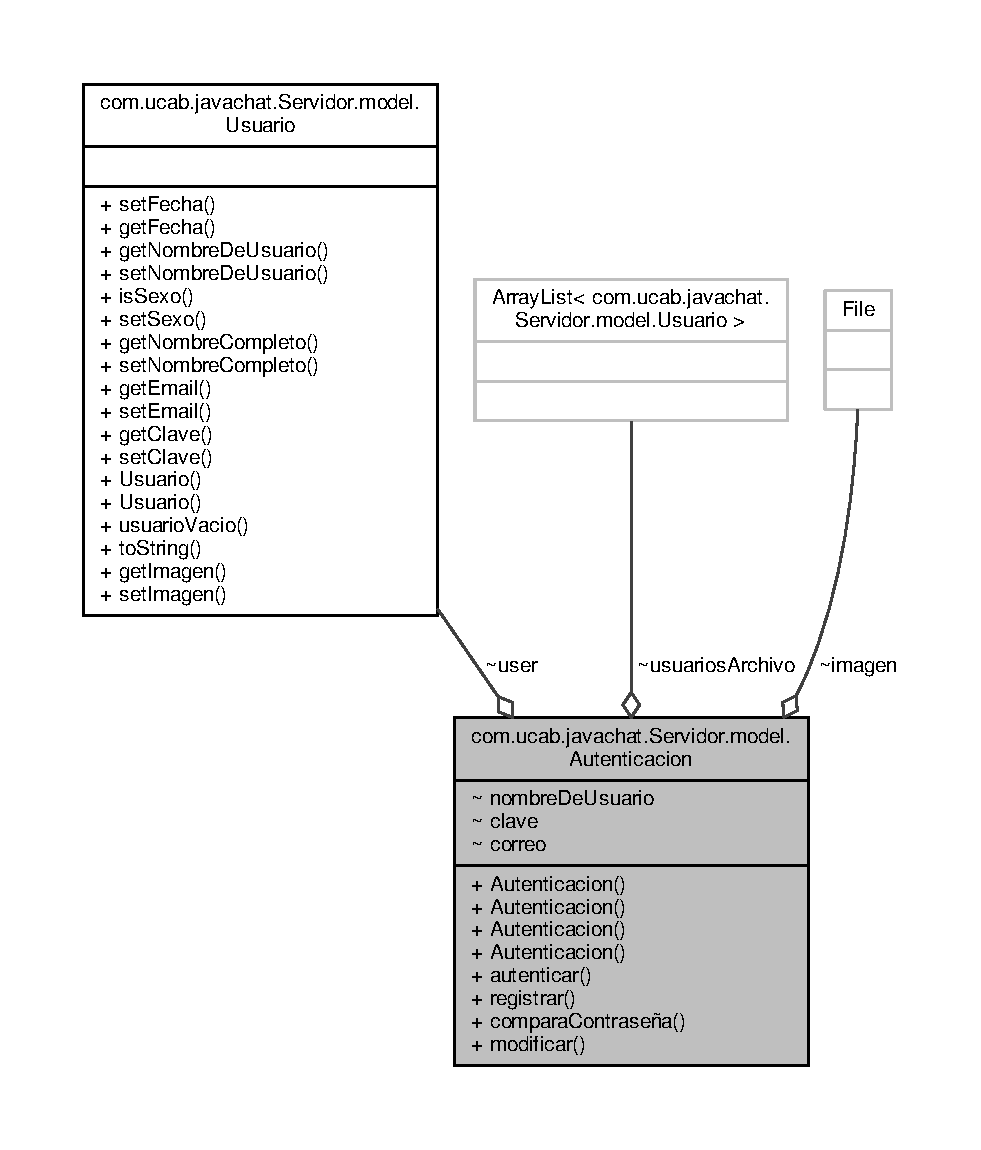
\includegraphics[width=350pt]{dc/dd4/classcom_1_1ucab_1_1javachat_1_1_servidor_1_1model_1_1_autenticacion__coll__graph}
\end{center}
\end{figure}
\subsection*{Métodos públicos}
\begin{DoxyCompactItemize}
\item 
\hyperlink{classcom_1_1ucab_1_1javachat_1_1_servidor_1_1model_1_1_autenticacion_acf6d86eec7551760ec91cc2ad09b5e3d}{Autenticacion} (\hyperlink{classcom_1_1ucab_1_1javachat_1_1_servidor_1_1model_1_1_usuario}{Usuario} user)
\item 
\hyperlink{classcom_1_1ucab_1_1javachat_1_1_servidor_1_1model_1_1_autenticacion_ae16e9a2db61ce5528fc5d024dec17092}{Autenticacion} (String nombre\-De\-Usuario, String clave, File imagen)
\item 
\hyperlink{classcom_1_1ucab_1_1javachat_1_1_servidor_1_1model_1_1_autenticacion_a58448a0f8c2cd4186dc2bf97ef81e2f7}{Autenticacion} (\hyperlink{classcom_1_1ucab_1_1javachat_1_1_servidor_1_1model_1_1_usuario}{Usuario} datos\-Modificados, String nombre\-Original)
\item 
\hypertarget{classcom_1_1ucab_1_1javachat_1_1_servidor_1_1model_1_1_autenticacion_a73bb46aee6ae1f6741ebb4cf73763efc}{{\bfseries Autenticacion} (String correo, File imagen)}\label{classcom_1_1ucab_1_1javachat_1_1_servidor_1_1model_1_1_autenticacion_a73bb46aee6ae1f6741ebb4cf73763efc}

\item 
\hyperlink{classcom_1_1ucab_1_1javachat_1_1_servidor_1_1model_1_1_usuario}{Usuario} \hyperlink{classcom_1_1ucab_1_1javachat_1_1_servidor_1_1model_1_1_autenticacion_abd542a51e7aca4eb713e823a82b83673}{autenticar} ()
\item 
int \hyperlink{classcom_1_1ucab_1_1javachat_1_1_servidor_1_1model_1_1_autenticacion_a14e19bd0d14451bb87fd62bdd74b15d7}{registrar} ()
\item 
\hypertarget{classcom_1_1ucab_1_1javachat_1_1_servidor_1_1model_1_1_autenticacion_ae18b837b59ef28f09723e6d772b5d26d}{String {\bfseries compara\-Contraseña} ()}\label{classcom_1_1ucab_1_1javachat_1_1_servidor_1_1model_1_1_autenticacion_ae18b837b59ef28f09723e6d772b5d26d}

\item 
\hypertarget{classcom_1_1ucab_1_1javachat_1_1_servidor_1_1model_1_1_autenticacion_a8c809a9a3e8bc1cf8590aa6ec6a45285}{int {\bfseries modificar} ()}\label{classcom_1_1ucab_1_1javachat_1_1_servidor_1_1model_1_1_autenticacion_a8c809a9a3e8bc1cf8590aa6ec6a45285}

\end{DoxyCompactItemize}


\subsection{Descripción detallada}
Clase encargada de la autenticacion del usuario en el sistema contrastando los datos recibidos con los almacenados en el servidor. Se encarga ademas de realizar las validaciones necesarias del lado del servidor y de comprobar los valores unicos \begin{DoxyAuthor}{Autor}
Grupo 3 -\/ A. Rodriguez, I. Teixeira, L. Valladares, D. Suarez 
\end{DoxyAuthor}


Definición en la línea 13 del archivo Autenticacion.\-java.



\subsection{Documentación del constructor y destructor}
\hypertarget{classcom_1_1ucab_1_1javachat_1_1_servidor_1_1model_1_1_autenticacion_acf6d86eec7551760ec91cc2ad09b5e3d}{\index{com\-::ucab\-::javachat\-::\-Servidor\-::model\-::\-Autenticacion@{com\-::ucab\-::javachat\-::\-Servidor\-::model\-::\-Autenticacion}!Autenticacion@{Autenticacion}}
\index{Autenticacion@{Autenticacion}!com::ucab::javachat::Servidor::model::Autenticacion@{com\-::ucab\-::javachat\-::\-Servidor\-::model\-::\-Autenticacion}}
\subsubsection[{Autenticacion}]{\setlength{\rightskip}{0pt plus 5cm}com.\-ucab.\-javachat.\-Servidor.\-model.\-Autenticacion.\-Autenticacion (
\begin{DoxyParamCaption}
\item[{{\bf Usuario}}]{user}
\end{DoxyParamCaption}
)}}\label{classcom_1_1ucab_1_1javachat_1_1_servidor_1_1model_1_1_autenticacion_acf6d86eec7551760ec91cc2ad09b5e3d}
Constructor para el registro de un nuevo usuario. 
\begin{DoxyParams}{Parámetros}
{\em user} & -\/ El usuario a registrar \\
\hline
\end{DoxyParams}


Definición en la línea 24 del archivo Autenticacion.\-java.

\hypertarget{classcom_1_1ucab_1_1javachat_1_1_servidor_1_1model_1_1_autenticacion_ae16e9a2db61ce5528fc5d024dec17092}{\index{com\-::ucab\-::javachat\-::\-Servidor\-::model\-::\-Autenticacion@{com\-::ucab\-::javachat\-::\-Servidor\-::model\-::\-Autenticacion}!Autenticacion@{Autenticacion}}
\index{Autenticacion@{Autenticacion}!com::ucab::javachat::Servidor::model::Autenticacion@{com\-::ucab\-::javachat\-::\-Servidor\-::model\-::\-Autenticacion}}
\subsubsection[{Autenticacion}]{\setlength{\rightskip}{0pt plus 5cm}com.\-ucab.\-javachat.\-Servidor.\-model.\-Autenticacion.\-Autenticacion (
\begin{DoxyParamCaption}
\item[{String}]{nombre\-De\-Usuario, }
\item[{String}]{clave, }
\item[{File}]{imagen}
\end{DoxyParamCaption}
)}}\label{classcom_1_1ucab_1_1javachat_1_1_servidor_1_1model_1_1_autenticacion_ae16e9a2db61ce5528fc5d024dec17092}
Constructor para el inicio de sesion de un usuario. 
\begin{DoxyParams}{Parámetros}
{\em nombre\-De\-Usuario} & -\/ nombre o correo del usuario que iniciar sesion \\
\hline
{\em clave} & -\/ clave del usuario que iniciara sesion \\
\hline
\end{DoxyParams}


Definición en la línea 34 del archivo Autenticacion.\-java.

\hypertarget{classcom_1_1ucab_1_1javachat_1_1_servidor_1_1model_1_1_autenticacion_a58448a0f8c2cd4186dc2bf97ef81e2f7}{\index{com\-::ucab\-::javachat\-::\-Servidor\-::model\-::\-Autenticacion@{com\-::ucab\-::javachat\-::\-Servidor\-::model\-::\-Autenticacion}!Autenticacion@{Autenticacion}}
\index{Autenticacion@{Autenticacion}!com::ucab::javachat::Servidor::model::Autenticacion@{com\-::ucab\-::javachat\-::\-Servidor\-::model\-::\-Autenticacion}}
\subsubsection[{Autenticacion}]{\setlength{\rightskip}{0pt plus 5cm}com.\-ucab.\-javachat.\-Servidor.\-model.\-Autenticacion.\-Autenticacion (
\begin{DoxyParamCaption}
\item[{{\bf Usuario}}]{datos\-Modificados, }
\item[{String}]{nombre\-Original}
\end{DoxyParamCaption}
)}}\label{classcom_1_1ucab_1_1javachat_1_1_servidor_1_1model_1_1_autenticacion_a58448a0f8c2cd4186dc2bf97ef81e2f7}
Constructor para la modificación de datos de un usuario 
\begin{DoxyParams}{Parámetros}
{\em datos\-Modificados} & -\/ un objeto del tipo usuario con los datos del usuario modificados \\
\hline
{\em nombre\-Original} & -\/ el nombre actual del usuario para buscarlo \\
\hline
\end{DoxyParams}


Definición en la línea 46 del archivo Autenticacion.\-java.



\subsection{Documentación de las funciones miembro}
\hypertarget{classcom_1_1ucab_1_1javachat_1_1_servidor_1_1model_1_1_autenticacion_abd542a51e7aca4eb713e823a82b83673}{\index{com\-::ucab\-::javachat\-::\-Servidor\-::model\-::\-Autenticacion@{com\-::ucab\-::javachat\-::\-Servidor\-::model\-::\-Autenticacion}!autenticar@{autenticar}}
\index{autenticar@{autenticar}!com::ucab::javachat::Servidor::model::Autenticacion@{com\-::ucab\-::javachat\-::\-Servidor\-::model\-::\-Autenticacion}}
\subsubsection[{autenticar}]{\setlength{\rightskip}{0pt plus 5cm}{\bf Usuario} com.\-ucab.\-javachat.\-Servidor.\-model.\-Autenticacion.\-autenticar (
\begin{DoxyParamCaption}
{}
\end{DoxyParamCaption}
)}}\label{classcom_1_1ucab_1_1javachat_1_1_servidor_1_1model_1_1_autenticacion_abd542a51e7aca4eb713e823a82b83673}
Realiza el proceso de autenticacion del usuario en el sistema contrastando sus datos con los almacenados en el sistema \begin{DoxyReturn}{Devuelve}
Verdadero cuando el usuario existe, falso en cualquier otro caso 
\end{DoxyReturn}


Definición en la línea 62 del archivo Autenticacion.\-java.

\hypertarget{classcom_1_1ucab_1_1javachat_1_1_servidor_1_1model_1_1_autenticacion_a14e19bd0d14451bb87fd62bdd74b15d7}{\index{com\-::ucab\-::javachat\-::\-Servidor\-::model\-::\-Autenticacion@{com\-::ucab\-::javachat\-::\-Servidor\-::model\-::\-Autenticacion}!registrar@{registrar}}
\index{registrar@{registrar}!com::ucab::javachat::Servidor::model::Autenticacion@{com\-::ucab\-::javachat\-::\-Servidor\-::model\-::\-Autenticacion}}
\subsubsection[{registrar}]{\setlength{\rightskip}{0pt plus 5cm}int com.\-ucab.\-javachat.\-Servidor.\-model.\-Autenticacion.\-registrar (
\begin{DoxyParamCaption}
{}
\end{DoxyParamCaption}
)}}\label{classcom_1_1ucab_1_1javachat_1_1_servidor_1_1model_1_1_autenticacion_a14e19bd0d14451bb87fd62bdd74b15d7}
Realiza el proceso de registro de usuario, almacenando el nuevo usuario en el archiv con comprobacion previa si el correo o el nombre de usuario ya estan registrados \begin{DoxyReturn}{Devuelve}
Verdadero si se registro el usuario, falso en cualquier otro caso 
\end{DoxyReturn}


Definición en la línea 88 del archivo Autenticacion.\-java.



La documentación para esta clase fue generada a partir del siguiente fichero\-:\begin{DoxyCompactItemize}
\item 
Chat-\/\-Codigo-\/\-Morse/\-Chat\-Morse/src/com/ucab/javachat/\-Servidor/model/Autenticacion.\-java\end{DoxyCompactItemize}

\hypertarget{classcom_1_1ucab_1_1javachat_1_1_cliente_1_1model_1_1_cliente}{\section{Referencia de la Clase com.\-ucab.\-javachat.\-Cliente.\-model.\-Cliente}
\label{classcom_1_1ucab_1_1javachat_1_1_cliente_1_1model_1_1_cliente}\index{com.\-ucab.\-javachat.\-Cliente.\-model.\-Cliente@{com.\-ucab.\-javachat.\-Cliente.\-model.\-Cliente}}
}


Diagrama de colaboración para com.\-ucab.\-javachat.\-Cliente.\-model.\-Cliente\-:
\nopagebreak
\begin{figure}[H]
\begin{center}
\leavevmode
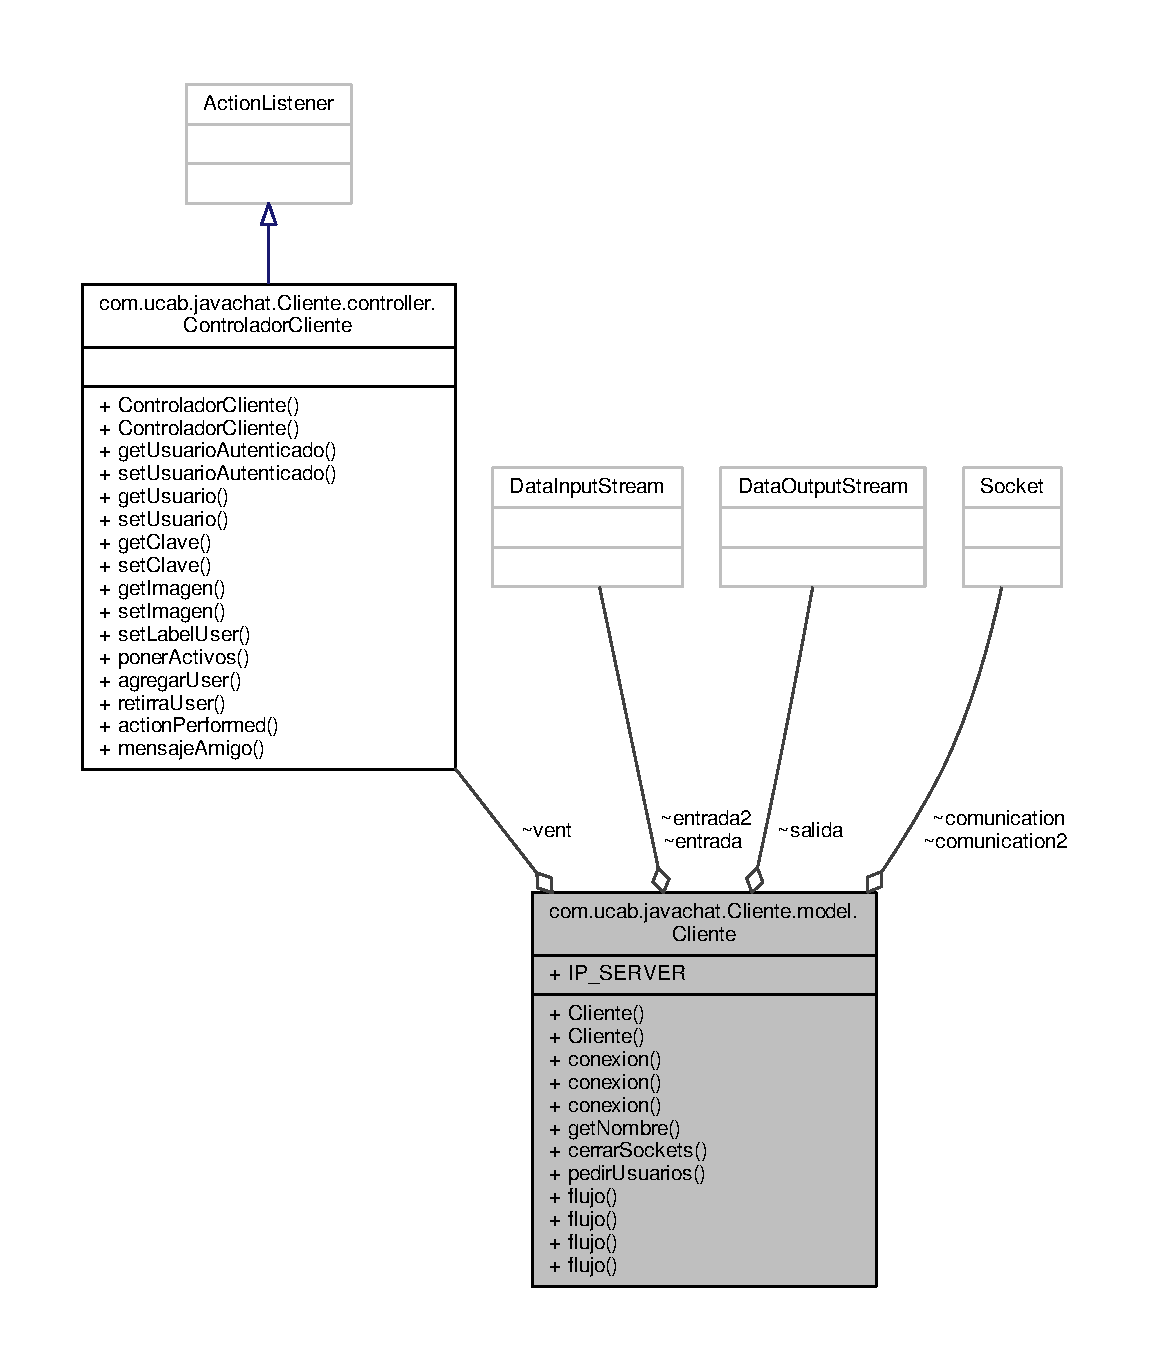
\includegraphics[width=350pt]{d4/d13/classcom_1_1ucab_1_1javachat_1_1_cliente_1_1model_1_1_cliente__coll__graph}
\end{center}
\end{figure}
\subsection*{Métodos públicos}
\begin{DoxyCompactItemize}
\item 
\hyperlink{classcom_1_1ucab_1_1javachat_1_1_cliente_1_1model_1_1_cliente_a96a7afffdedcb21e2fa287056460c163}{Cliente} (\hyperlink{classcom_1_1ucab_1_1javachat_1_1_cliente_1_1controller_1_1_controlador_cliente}{Controlador\-Cliente} vent)  throws I\-O\-Exception    
\item 
\hyperlink{classcom_1_1ucab_1_1javachat_1_1_cliente_1_1model_1_1_usuario}{Usuario} \hyperlink{classcom_1_1ucab_1_1javachat_1_1_cliente_1_1model_1_1_cliente_ad187c584feac2fbaddf36074a7d7ee64}{conexion} (String nombre, String clave, File imagen)  throws I\-O\-Exception 
\item 
int \hyperlink{classcom_1_1ucab_1_1javachat_1_1_cliente_1_1model_1_1_cliente_a56292074d2a5b409b5056db1d07168bd}{conexion} (\hyperlink{classcom_1_1ucab_1_1javachat_1_1_cliente_1_1model_1_1_usuario}{Usuario} nuevo\-Usuario)  throws I\-O\-Exception 
\item 
\hypertarget{classcom_1_1ucab_1_1javachat_1_1_cliente_1_1model_1_1_cliente_a8ff5750a0dd7b1e68373f49be2662ca3}{boolean {\bfseries conexion} (String correo, File imagen)  throws I\-O\-Exception }\label{classcom_1_1ucab_1_1javachat_1_1_cliente_1_1model_1_1_cliente_a8ff5750a0dd7b1e68373f49be2662ca3}

\item 
\hypertarget{classcom_1_1ucab_1_1javachat_1_1_cliente_1_1model_1_1_cliente_a2f102f095b1bd161a90a3d13f1285eeb}{String {\bfseries get\-Nombre} ()}\label{classcom_1_1ucab_1_1javachat_1_1_cliente_1_1model_1_1_cliente_a2f102f095b1bd161a90a3d13f1285eeb}

\item 
\hypertarget{classcom_1_1ucab_1_1javachat_1_1_cliente_1_1model_1_1_cliente_ada58df8e38b7252aee067a222029f1bb}{void {\bfseries cerrar\-Sockets} ()}\label{classcom_1_1ucab_1_1javachat_1_1_cliente_1_1model_1_1_cliente_ada58df8e38b7252aee067a222029f1bb}

\item 
Vector$<$ String $>$ \hyperlink{classcom_1_1ucab_1_1javachat_1_1_cliente_1_1model_1_1_cliente_ae828d3c313aa6e5a38129433baf036ab}{pedir\-Usuarios} ()
\item 
void \hyperlink{classcom_1_1ucab_1_1javachat_1_1_cliente_1_1model_1_1_cliente_a6a000d747c356a8fc093fb9299185b0c}{flujo} (Vector$<$ String $>$ amigos, String mens, String emisor)
\item 
int \hyperlink{classcom_1_1ucab_1_1javachat_1_1_cliente_1_1model_1_1_cliente_ac98f059bfb01929a8fcae393be001e07}{flujo} (\hyperlink{classcom_1_1ucab_1_1javachat_1_1_cliente_1_1model_1_1_usuario}{Usuario} usuario)
\item 
\hypertarget{classcom_1_1ucab_1_1javachat_1_1_cliente_1_1model_1_1_cliente_ae3d51eeea6685fce41818e231c28fd11}{boolean {\bfseries flujo} (String correo, File imagen)}\label{classcom_1_1ucab_1_1javachat_1_1_cliente_1_1model_1_1_cliente_ae3d51eeea6685fce41818e231c28fd11}

\item 
int \hyperlink{classcom_1_1ucab_1_1javachat_1_1_cliente_1_1model_1_1_cliente_ae9914153c2e3e6fc5a659b5aa1022c67}{flujo} (\hyperlink{classcom_1_1ucab_1_1javachat_1_1_cliente_1_1model_1_1_usuario}{Usuario} usuario, String nombre\-Original, boolean imagen\-Cambia)
\end{DoxyCompactItemize}
\subsection*{Atributos públicos estáticos}
\begin{DoxyCompactItemize}
\item 
\hypertarget{classcom_1_1ucab_1_1javachat_1_1_cliente_1_1model_1_1_cliente_a5decf95cef7084b662f4a4d207f165a5}{static String {\bfseries I\-P\-\_\-\-S\-E\-R\-V\-E\-R}}\label{classcom_1_1ucab_1_1javachat_1_1_cliente_1_1model_1_1_cliente_a5decf95cef7084b662f4a4d207f165a5}

\end{DoxyCompactItemize}


\subsection{Descripción detallada}
Modelo del cliente que utiliza el chat. Crea la comunicar mediante sockets con el sevidor.

\begin{DoxyAuthor}{Autores}
Grupo 3 -\/ A. Rodriguez, I. Teixeira, L. Valladares, D. Suarez 
\end{DoxyAuthor}
\begin{DoxyVersion}{Versión}
2.\-0 
\end{DoxyVersion}


Definición en la línea 36 del archivo Cliente.\-java.



\subsection{Documentación del constructor y destructor}
\hypertarget{classcom_1_1ucab_1_1javachat_1_1_cliente_1_1model_1_1_cliente_a96a7afffdedcb21e2fa287056460c163}{\index{com\-::ucab\-::javachat\-::\-Cliente\-::model\-::\-Cliente@{com\-::ucab\-::javachat\-::\-Cliente\-::model\-::\-Cliente}!Cliente@{Cliente}}
\index{Cliente@{Cliente}!com::ucab::javachat::Cliente::model::Cliente@{com\-::ucab\-::javachat\-::\-Cliente\-::model\-::\-Cliente}}
\subsubsection[{Cliente}]{\setlength{\rightskip}{0pt plus 5cm}com.\-ucab.\-javachat.\-Cliente.\-model.\-Cliente.\-Cliente (
\begin{DoxyParamCaption}
\item[{{\bf Controlador\-Cliente}}]{vent}
\end{DoxyParamCaption}
) throws I\-O\-Exception}}\label{classcom_1_1ucab_1_1javachat_1_1_cliente_1_1model_1_1_cliente_a96a7afffdedcb21e2fa287056460c163}
Creates a new instance of \hyperlink{classcom_1_1ucab_1_1javachat_1_1_cliente_1_1model_1_1_cliente}{Cliente}. 

Definición en la línea 48 del archivo Cliente.\-java.



\subsection{Documentación de las funciones miembro}
\hypertarget{classcom_1_1ucab_1_1javachat_1_1_cliente_1_1model_1_1_cliente_ad187c584feac2fbaddf36074a7d7ee64}{\index{com\-::ucab\-::javachat\-::\-Cliente\-::model\-::\-Cliente@{com\-::ucab\-::javachat\-::\-Cliente\-::model\-::\-Cliente}!conexion@{conexion}}
\index{conexion@{conexion}!com::ucab::javachat::Cliente::model::Cliente@{com\-::ucab\-::javachat\-::\-Cliente\-::model\-::\-Cliente}}
\subsubsection[{conexion}]{\setlength{\rightskip}{0pt plus 5cm}{\bf Usuario} com.\-ucab.\-javachat.\-Cliente.\-model.\-Cliente.\-conexion (
\begin{DoxyParamCaption}
\item[{String}]{nombre, }
\item[{String}]{clave, }
\item[{File}]{imagen}
\end{DoxyParamCaption}
) throws I\-O\-Exception}}\label{classcom_1_1ucab_1_1javachat_1_1_cliente_1_1model_1_1_cliente_ad187c584feac2fbaddf36074a7d7ee64}
Metodo que inicializa los sockets con el servidor y envia el nombre de usuario y la contraseña para la autenticacion en el servidor


\begin{DoxyParams}{Parámetros}
{\em nombre} & nombre de usuario \\
\hline
{\em clave} & clave del usuario (cifrada) \\
\hline
\end{DoxyParams}

\begin{DoxyExceptions}{Excepciones}
{\em I\-O\-Exception} & \\
\hline
\end{DoxyExceptions}


Definición en la línea 65 del archivo Cliente.\-java.



Gráfico de llamadas a esta función\-:
\nopagebreak
\begin{figure}[H]
\begin{center}
\leavevmode
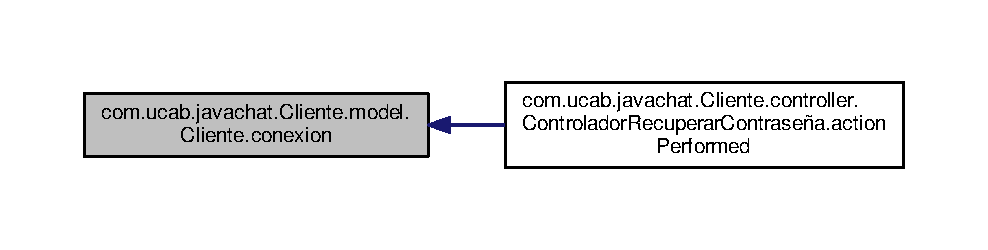
\includegraphics[width=350pt]{de/df9/classcom_1_1ucab_1_1javachat_1_1_cliente_1_1model_1_1_cliente_ad187c584feac2fbaddf36074a7d7ee64_icgraph}
\end{center}
\end{figure}


\hypertarget{classcom_1_1ucab_1_1javachat_1_1_cliente_1_1model_1_1_cliente_a56292074d2a5b409b5056db1d07168bd}{\index{com\-::ucab\-::javachat\-::\-Cliente\-::model\-::\-Cliente@{com\-::ucab\-::javachat\-::\-Cliente\-::model\-::\-Cliente}!conexion@{conexion}}
\index{conexion@{conexion}!com::ucab::javachat::Cliente::model::Cliente@{com\-::ucab\-::javachat\-::\-Cliente\-::model\-::\-Cliente}}
\subsubsection[{conexion}]{\setlength{\rightskip}{0pt plus 5cm}int com.\-ucab.\-javachat.\-Cliente.\-model.\-Cliente.\-conexion (
\begin{DoxyParamCaption}
\item[{{\bf Usuario}}]{nuevo\-Usuario}
\end{DoxyParamCaption}
) throws I\-O\-Exception}}\label{classcom_1_1ucab_1_1javachat_1_1_cliente_1_1model_1_1_cliente_a56292074d2a5b409b5056db1d07168bd}
Envia los datos del nuevo usuario al servidor para realizar las validaciones necesarias del lado del servidor y su almacenamiento en el archivo para el registro 
\begin{DoxyParams}{Parámetros}
{\em nuevo\-Usuario} & -\/ Datos del nuevo usuario a registrar en el sistema \\
\hline
\end{DoxyParams}

\begin{DoxyExceptions}{Excepciones}
{\em I\-O\-Exception} & \\
\hline
\end{DoxyExceptions}


Definición en la línea 109 del archivo Cliente.\-java.



Gráfico de llamadas para esta función\-:
\nopagebreak
\begin{figure}[H]
\begin{center}
\leavevmode
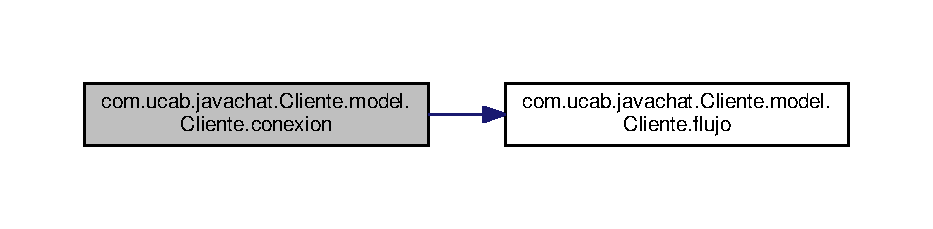
\includegraphics[width=350pt]{de/df9/classcom_1_1ucab_1_1javachat_1_1_cliente_1_1model_1_1_cliente_a56292074d2a5b409b5056db1d07168bd_cgraph}
\end{center}
\end{figure}


\hypertarget{classcom_1_1ucab_1_1javachat_1_1_cliente_1_1model_1_1_cliente_a6a000d747c356a8fc093fb9299185b0c}{\index{com\-::ucab\-::javachat\-::\-Cliente\-::model\-::\-Cliente@{com\-::ucab\-::javachat\-::\-Cliente\-::model\-::\-Cliente}!flujo@{flujo}}
\index{flujo@{flujo}!com::ucab::javachat::Cliente::model::Cliente@{com\-::ucab\-::javachat\-::\-Cliente\-::model\-::\-Cliente}}
\subsubsection[{flujo}]{\setlength{\rightskip}{0pt plus 5cm}void com.\-ucab.\-javachat.\-Cliente.\-model.\-Cliente.\-flujo (
\begin{DoxyParamCaption}
\item[{Vector$<$ String $>$}]{amigos, }
\item[{String}]{mens, }
\item[{String}]{emisor}
\end{DoxyParamCaption}
)}}\label{classcom_1_1ucab_1_1javachat_1_1_cliente_1_1model_1_1_cliente_a6a000d747c356a8fc093fb9299185b0c}
Este metodo envia un mensaje a todos los usuarios que estan en una ventana grupal y privada. 
\begin{DoxyParams}{Parámetros}
{\em amigos} & -\/ Usuarios en la ventana privada. \\
\hline
{\em mens} & -\/ Mensaje a enviar. \\
\hline
\end{DoxyParams}


Definición en la línea 178 del archivo Cliente.\-java.



Gráfico de llamadas a esta función\-:
\nopagebreak
\begin{figure}[H]
\begin{center}
\leavevmode
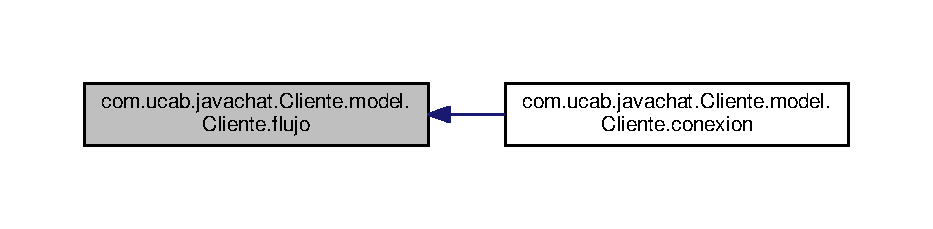
\includegraphics[width=350pt]{de/df9/classcom_1_1ucab_1_1javachat_1_1_cliente_1_1model_1_1_cliente_a6a000d747c356a8fc093fb9299185b0c_icgraph}
\end{center}
\end{figure}


\hypertarget{classcom_1_1ucab_1_1javachat_1_1_cliente_1_1model_1_1_cliente_ac98f059bfb01929a8fcae393be001e07}{\index{com\-::ucab\-::javachat\-::\-Cliente\-::model\-::\-Cliente@{com\-::ucab\-::javachat\-::\-Cliente\-::model\-::\-Cliente}!flujo@{flujo}}
\index{flujo@{flujo}!com::ucab::javachat::Cliente::model::Cliente@{com\-::ucab\-::javachat\-::\-Cliente\-::model\-::\-Cliente}}
\subsubsection[{flujo}]{\setlength{\rightskip}{0pt plus 5cm}int com.\-ucab.\-javachat.\-Cliente.\-model.\-Cliente.\-flujo (
\begin{DoxyParamCaption}
\item[{{\bf Usuario}}]{usuario}
\end{DoxyParamCaption}
)}}\label{classcom_1_1ucab_1_1javachat_1_1_cliente_1_1model_1_1_cliente_ac98f059bfb01929a8fcae393be001e07}
Este metodo se encarga de enviar una instancia del objeto usuario al servidor, para esto se crea un objeto json en el que se añaden los datos del usuario. 
\begin{DoxyParams}{Parámetros}
{\em usuario} & -\/ Objeto que contiene los datos de un usuario que esta en el proceso de registro. \\
\hline
\end{DoxyParams}


Definición en la línea 197 del archivo Cliente.\-java.

\hypertarget{classcom_1_1ucab_1_1javachat_1_1_cliente_1_1model_1_1_cliente_ae9914153c2e3e6fc5a659b5aa1022c67}{\index{com\-::ucab\-::javachat\-::\-Cliente\-::model\-::\-Cliente@{com\-::ucab\-::javachat\-::\-Cliente\-::model\-::\-Cliente}!flujo@{flujo}}
\index{flujo@{flujo}!com::ucab::javachat::Cliente::model::Cliente@{com\-::ucab\-::javachat\-::\-Cliente\-::model\-::\-Cliente}}
\subsubsection[{flujo}]{\setlength{\rightskip}{0pt plus 5cm}int com.\-ucab.\-javachat.\-Cliente.\-model.\-Cliente.\-flujo (
\begin{DoxyParamCaption}
\item[{{\bf Usuario}}]{usuario, }
\item[{String}]{nombre\-Original, }
\item[{boolean}]{imagen\-Cambia}
\end{DoxyParamCaption}
)}}\label{classcom_1_1ucab_1_1javachat_1_1_cliente_1_1model_1_1_cliente_ae9914153c2e3e6fc5a659b5aa1022c67}
este metodo se encarga de enviar un objeto de tipo \hyperlink{classcom_1_1ucab_1_1javachat_1_1_cliente_1_1model_1_1_usuario}{Usuario} al servidor 
\begin{DoxyParams}{Parámetros}
{\em usuario} & Objeto que contiene los datos de un usuario que esta en el proceso de registro. \\
\hline
{\em entrar} & \\
\hline
\end{DoxyParams}
\begin{DoxyReturn}{Devuelve}

\end{DoxyReturn}


Definición en la línea 244 del archivo Cliente.\-java.

\hypertarget{classcom_1_1ucab_1_1javachat_1_1_cliente_1_1model_1_1_cliente_ae828d3c313aa6e5a38129433baf036ab}{\index{com\-::ucab\-::javachat\-::\-Cliente\-::model\-::\-Cliente@{com\-::ucab\-::javachat\-::\-Cliente\-::model\-::\-Cliente}!pedir\-Usuarios@{pedir\-Usuarios}}
\index{pedir\-Usuarios@{pedir\-Usuarios}!com::ucab::javachat::Cliente::model::Cliente@{com\-::ucab\-::javachat\-::\-Cliente\-::model\-::\-Cliente}}
\subsubsection[{pedir\-Usuarios}]{\setlength{\rightskip}{0pt plus 5cm}Vector$<$String$>$ com.\-ucab.\-javachat.\-Cliente.\-model.\-Cliente.\-pedir\-Usuarios (
\begin{DoxyParamCaption}
{}
\end{DoxyParamCaption}
)}}\label{classcom_1_1ucab_1_1javachat_1_1_cliente_1_1model_1_1_cliente_ae828d3c313aa6e5a38129433baf036ab}
Este metodo al ser invocado se encarga de enviar la lista de todos los usarios conectados. \begin{DoxyReturn}{Devuelve}
Vector con los usuarios conectados. 
\end{DoxyReturn}


Definición en la línea 160 del archivo Cliente.\-java.



La documentación para esta clase fue generada a partir del siguiente fichero\-:\begin{DoxyCompactItemize}
\item 
Chat-\/\-Codigo-\/\-Morse/\-Chat\-Morse/src/com/ucab/javachat/\-Cliente/model/Cliente.\-java\end{DoxyCompactItemize}

\hypertarget{classcom_1_1ucab_1_1javachat_1_1_cliente_1_1model_1_1_codigo_morse}{\section{Referencia de la Clase com.\-ucab.\-javachat.\-Cliente.\-model.\-Codigo\-Morse}
\label{classcom_1_1ucab_1_1javachat_1_1_cliente_1_1model_1_1_codigo_morse}\index{com.\-ucab.\-javachat.\-Cliente.\-model.\-Codigo\-Morse@{com.\-ucab.\-javachat.\-Cliente.\-model.\-Codigo\-Morse}}
}


Diagrama de colaboración para com.\-ucab.\-javachat.\-Cliente.\-model.\-Codigo\-Morse\-:\nopagebreak
\begin{figure}[H]
\begin{center}
\leavevmode
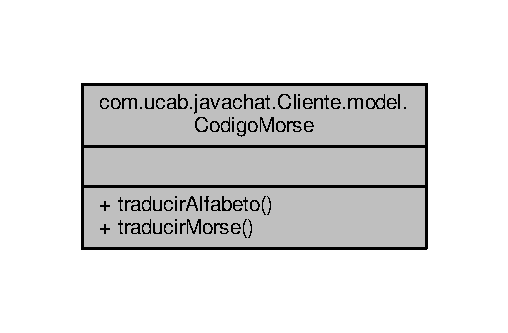
\includegraphics[width=244pt]{classcom_1_1ucab_1_1javachat_1_1_cliente_1_1model_1_1_codigo_morse__coll__graph}
\end{center}
\end{figure}
\subsection*{Métodos públicos estáticos}
\begin{DoxyCompactItemize}
\item 
static String \hyperlink{classcom_1_1ucab_1_1javachat_1_1_cliente_1_1model_1_1_codigo_morse_a043b70b087c4b8b530dc3eb03289fc98}{traducir\-Alfabeto} (String mensaje)
\item 
static String \hyperlink{classcom_1_1ucab_1_1javachat_1_1_cliente_1_1model_1_1_codigo_morse_aaff032c4492797c05151156469193c35}{traducir\-Morse} (String mensaje)
\end{DoxyCompactItemize}


\subsection{Descripción detallada}
Esta clase se encarga de traducir un texto a codigo morse y viceversa \begin{DoxyAuthor}{Autor}
Grupo 3 -\/ A. Rodriguez, I. Teixeira, L. Valladares, D. Suarez 
\end{DoxyAuthor}


Definición en la línea 8 del archivo Codigo\-Morse.\-java.



\subsection{Documentación de las funciones miembro}
\hypertarget{classcom_1_1ucab_1_1javachat_1_1_cliente_1_1model_1_1_codigo_morse_a043b70b087c4b8b530dc3eb03289fc98}{\index{com\-::ucab\-::javachat\-::\-Cliente\-::model\-::\-Codigo\-Morse@{com\-::ucab\-::javachat\-::\-Cliente\-::model\-::\-Codigo\-Morse}!traducir\-Alfabeto@{traducir\-Alfabeto}}
\index{traducir\-Alfabeto@{traducir\-Alfabeto}!com::ucab::javachat::Cliente::model::CodigoMorse@{com\-::ucab\-::javachat\-::\-Cliente\-::model\-::\-Codigo\-Morse}}
\subsubsection[{traducir\-Alfabeto}]{\setlength{\rightskip}{0pt plus 5cm}static String com.\-ucab.\-javachat.\-Cliente.\-model.\-Codigo\-Morse.\-traducir\-Alfabeto (
\begin{DoxyParamCaption}
\item[{String}]{mensaje}
\end{DoxyParamCaption}
)\hspace{0.3cm}{\ttfamily [static]}}}\label{classcom_1_1ucab_1_1javachat_1_1_cliente_1_1model_1_1_codigo_morse_a043b70b087c4b8b530dc3eb03289fc98}
Este metodo se encarga de transformar un texto a codigo morse 
\begin{DoxyParams}{Parámetros}
{\em mensaje} & Mensaje a traducir \\
\hline
\end{DoxyParams}
\begin{DoxyReturn}{Devuelve}
morse 
\end{DoxyReturn}


Definición en la línea 15 del archivo Codigo\-Morse.\-java.

\hypertarget{classcom_1_1ucab_1_1javachat_1_1_cliente_1_1model_1_1_codigo_morse_aaff032c4492797c05151156469193c35}{\index{com\-::ucab\-::javachat\-::\-Cliente\-::model\-::\-Codigo\-Morse@{com\-::ucab\-::javachat\-::\-Cliente\-::model\-::\-Codigo\-Morse}!traducir\-Morse@{traducir\-Morse}}
\index{traducir\-Morse@{traducir\-Morse}!com::ucab::javachat::Cliente::model::CodigoMorse@{com\-::ucab\-::javachat\-::\-Cliente\-::model\-::\-Codigo\-Morse}}
\subsubsection[{traducir\-Morse}]{\setlength{\rightskip}{0pt plus 5cm}static String com.\-ucab.\-javachat.\-Cliente.\-model.\-Codigo\-Morse.\-traducir\-Morse (
\begin{DoxyParamCaption}
\item[{String}]{mensaje}
\end{DoxyParamCaption}
)\hspace{0.3cm}{\ttfamily [static]}}}\label{classcom_1_1ucab_1_1javachat_1_1_cliente_1_1model_1_1_codigo_morse_aaff032c4492797c05151156469193c35}
Este metodo traduce el codigo morse a alfabeto 
\begin{DoxyParams}{Parámetros}
{\em mensaje} & \\
\hline
\end{DoxyParams}
\begin{DoxyReturn}{Devuelve}
morse 
\end{DoxyReturn}


Definición en la línea 101 del archivo Codigo\-Morse.\-java.



La documentación para esta clase fue generada a partir del siguiente fichero\-:\begin{DoxyCompactItemize}
\item 
Escritorio/\-Chat\-Morse/src/com/ucab/javachat/\-Cliente/model/\hyperlink{_codigo_morse_8java}{Codigo\-Morse.\-java}\end{DoxyCompactItemize}

\hypertarget{classcom_1_1ucab_1_1javachat_1_1_servidor_1_1model_1_1_comparar_imagenes}{\section{Referencia de la Clase com.\-ucab.\-javachat.\-Servidor.\-model.\-Comparar\-Imagenes}
\label{classcom_1_1ucab_1_1javachat_1_1_servidor_1_1model_1_1_comparar_imagenes}\index{com.\-ucab.\-javachat.\-Servidor.\-model.\-Comparar\-Imagenes@{com.\-ucab.\-javachat.\-Servidor.\-model.\-Comparar\-Imagenes}}
}


Diagrama de colaboración para com.\-ucab.\-javachat.\-Servidor.\-model.\-Comparar\-Imagenes\-:
\nopagebreak
\begin{figure}[H]
\begin{center}
\leavevmode
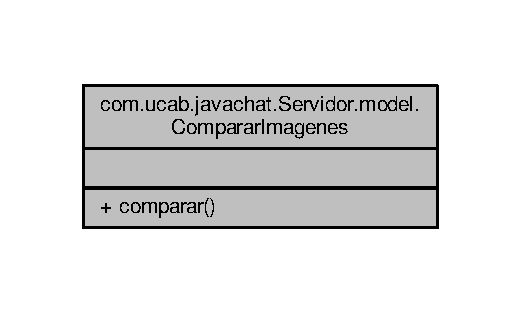
\includegraphics[width=250pt]{d7/d91/classcom_1_1ucab_1_1javachat_1_1_servidor_1_1model_1_1_comparar_imagenes__coll__graph}
\end{center}
\end{figure}
\subsection*{Métodos públicos estáticos}
\begin{DoxyCompactItemize}
\item 
\hypertarget{classcom_1_1ucab_1_1javachat_1_1_servidor_1_1model_1_1_comparar_imagenes_a35bd16d8d9c4c2bd3148cc5f1918f349}{static boolean {\bfseries comparar} (File imagen1, File imagen2)  throws I\-O\-Exception 	}\label{classcom_1_1ucab_1_1javachat_1_1_servidor_1_1model_1_1_comparar_imagenes_a35bd16d8d9c4c2bd3148cc5f1918f349}

\end{DoxyCompactItemize}


\subsection{Descripción detallada}
Desarrollado Por\-: Ing. Randy F. Amaya Email\-: \href{mailto:randy.amaya@uth.hn}{\tt randy.\-amaya@uth.\-hn}

www.\-computrachos.\-com La Comunidad Donde el Conocimiento Se Comparte!!! 

Definición en la línea 17 del archivo Comparar\-Imagenes.\-java.



La documentación para esta clase fue generada a partir del siguiente fichero\-:\begin{DoxyCompactItemize}
\item 
Chat-\/\-Codigo-\/\-Morse/\-Chat\-Morse/src/com/ucab/javachat/\-Servidor/model/Comparar\-Imagenes.\-java\end{DoxyCompactItemize}

\hypertarget{classcom_1_1ucab_1_1javachat_1_1_cliente_1_1controller_1_1_controlador_cliente}{\section{Referencia de la Clase com.\-ucab.\-javachat.\-Cliente.\-controller.\-Controlador\-Cliente}
\label{classcom_1_1ucab_1_1javachat_1_1_cliente_1_1controller_1_1_controlador_cliente}\index{com.\-ucab.\-javachat.\-Cliente.\-controller.\-Controlador\-Cliente@{com.\-ucab.\-javachat.\-Cliente.\-controller.\-Controlador\-Cliente}}
}


Diagrama de herencias de com.\-ucab.\-javachat.\-Cliente.\-controller.\-Controlador\-Cliente
\nopagebreak
\begin{figure}[H]
\begin{center}
\leavevmode
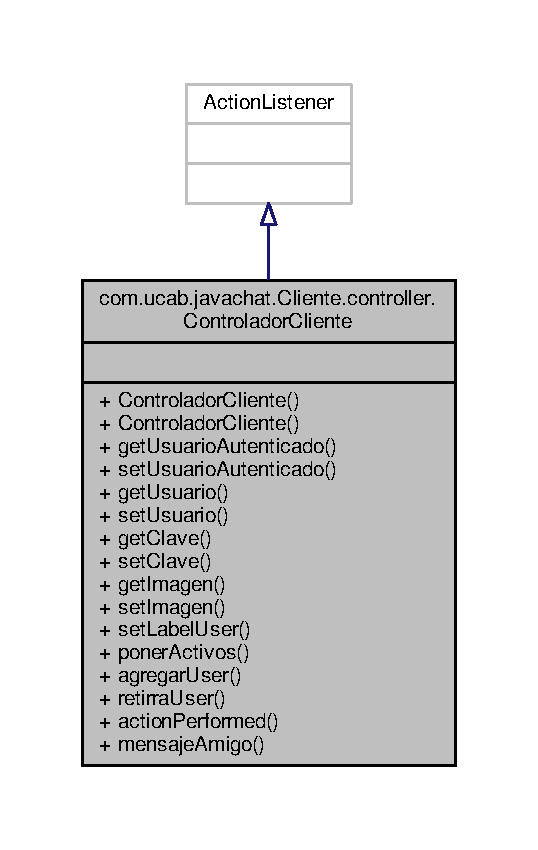
\includegraphics[width=258pt]{dd/d62/classcom_1_1ucab_1_1javachat_1_1_cliente_1_1controller_1_1_controlador_cliente__inherit__graph}
\end{center}
\end{figure}


Diagrama de colaboración para com.\-ucab.\-javachat.\-Cliente.\-controller.\-Controlador\-Cliente\-:
\nopagebreak
\begin{figure}[H]
\begin{center}
\leavevmode
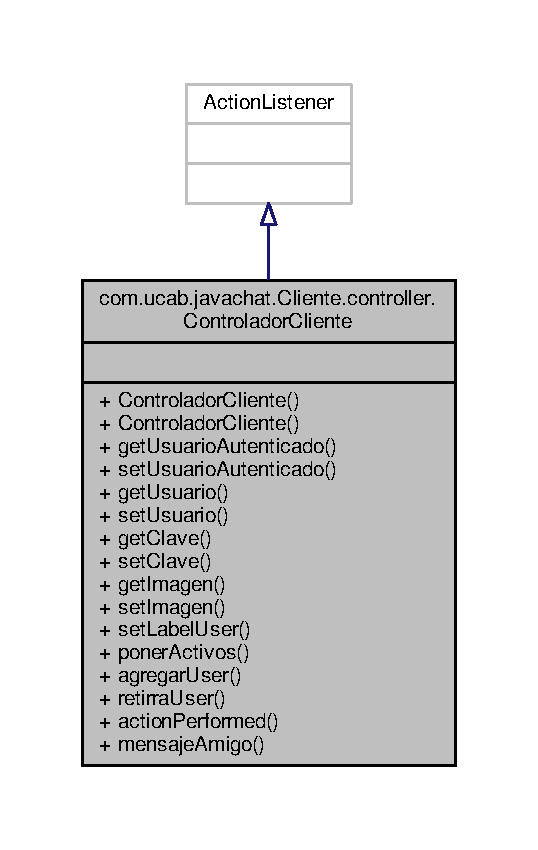
\includegraphics[width=258pt]{de/d44/classcom_1_1ucab_1_1javachat_1_1_cliente_1_1controller_1_1_controlador_cliente__coll__graph}
\end{center}
\end{figure}
\subsection*{Métodos públicos}
\begin{DoxyCompactItemize}
\item 
\hyperlink{classcom_1_1ucab_1_1javachat_1_1_cliente_1_1controller_1_1_controlador_cliente_a169ce22e78795bc739fde02d29afbf5a}{Controlador\-Cliente} (final \hyperlink{classcom_1_1ucab_1_1javachat_1_1_cliente_1_1view_1_1_vent_cliente}{Vent\-Cliente} ventana, \hyperlink{classcom_1_1ucab_1_1javachat_1_1_cliente_1_1controller_1_1_controlador_iniciar_sesion}{Controlador\-Iniciar\-Sesion} cont\-Sesion)
\item 
\hypertarget{classcom_1_1ucab_1_1javachat_1_1_cliente_1_1controller_1_1_controlador_cliente_ae11bb33a2245f1000c5df1834a360746}{{\bfseries Controlador\-Cliente} (final \hyperlink{classcom_1_1ucab_1_1javachat_1_1_cliente_1_1view_1_1_vent_cliente}{Vent\-Cliente} ventana, \hyperlink{classcom_1_1ucab_1_1javachat_1_1_cliente_1_1controller_1_1_controlador_registrar_usuario}{Controlador\-Registrar\-Usuario} cont\-Usuario)}\label{classcom_1_1ucab_1_1javachat_1_1_cliente_1_1controller_1_1_controlador_cliente_ae11bb33a2245f1000c5df1834a360746}

\item 
\hypertarget{classcom_1_1ucab_1_1javachat_1_1_cliente_1_1controller_1_1_controlador_cliente_a12ea6a6be82d2b5ce6bcc1fc6d4f3a73}{final \hyperlink{classcom_1_1ucab_1_1javachat_1_1_cliente_1_1model_1_1_usuario}{Usuario} {\bfseries get\-Usuario\-Autenticado} ()}\label{classcom_1_1ucab_1_1javachat_1_1_cliente_1_1controller_1_1_controlador_cliente_a12ea6a6be82d2b5ce6bcc1fc6d4f3a73}

\item 
\hypertarget{classcom_1_1ucab_1_1javachat_1_1_cliente_1_1controller_1_1_controlador_cliente_a32c622eb684b582d03d81ae98bf8be49}{final void {\bfseries set\-Usuario\-Autenticado} (\hyperlink{classcom_1_1ucab_1_1javachat_1_1_cliente_1_1model_1_1_usuario}{Usuario} usuario\-Autenticado)}\label{classcom_1_1ucab_1_1javachat_1_1_cliente_1_1controller_1_1_controlador_cliente_a32c622eb684b582d03d81ae98bf8be49}

\item 
final String \hyperlink{classcom_1_1ucab_1_1javachat_1_1_cliente_1_1controller_1_1_controlador_cliente_ada03c074086d0d54321cdf0347147397}{get\-Usuario} ()
\item 
final void \hyperlink{classcom_1_1ucab_1_1javachat_1_1_cliente_1_1controller_1_1_controlador_cliente_a29e6cb2c38d42517282ce2da900b3516}{set\-Usuario} (final String usuario)
\item 
final String \hyperlink{classcom_1_1ucab_1_1javachat_1_1_cliente_1_1controller_1_1_controlador_cliente_a3e147fa15044b926e8f496e15153e8f9}{get\-Clave} ()
\item 
final void \hyperlink{classcom_1_1ucab_1_1javachat_1_1_cliente_1_1controller_1_1_controlador_cliente_a8647e56fdb735f7abdef284b023e9f53}{set\-Clave} (final String clave)
\item 
final File \hyperlink{classcom_1_1ucab_1_1javachat_1_1_cliente_1_1controller_1_1_controlador_cliente_adb75ed57c31baca876b69990bbafb400}{get\-Imagen} ()
\item 
final void \hyperlink{classcom_1_1ucab_1_1javachat_1_1_cliente_1_1controller_1_1_controlador_cliente_a6e7b9e6c4a82829efbd0aae6c2658184}{set\-Imagen} (final File imagen)
\item 
final void \hyperlink{classcom_1_1ucab_1_1javachat_1_1_cliente_1_1controller_1_1_controlador_cliente_aa19a69efd4f74891f467345498ddcb39}{set\-Label\-User} ()
\item 
final void \hyperlink{classcom_1_1ucab_1_1javachat_1_1_cliente_1_1controller_1_1_controlador_cliente_a0ec86bb408cc78782346b4c01b95a7d6}{poner\-Activos} (final Vector$<$ String $>$ datos)
\item 
final void \hyperlink{classcom_1_1ucab_1_1javachat_1_1_cliente_1_1controller_1_1_controlador_cliente_a3aff80775389cf97755cd5c7db915603}{agregar\-User} (final String user)
\item 
final void \hyperlink{classcom_1_1ucab_1_1javachat_1_1_cliente_1_1controller_1_1_controlador_cliente_abb244f9e8904743e123c5e86a42c4710}{retirra\-User} (final String user)
\item 
final void \hyperlink{classcom_1_1ucab_1_1javachat_1_1_cliente_1_1controller_1_1_controlador_cliente_a132f8481c0894cdad40225f8541931a0}{action\-Performed} (final Action\-Event evt)
\item 
\hypertarget{classcom_1_1ucab_1_1javachat_1_1_cliente_1_1controller_1_1_controlador_cliente_aad384e7a7cfd86adf60b62591a5d49ff}{final void {\bfseries mensaje\-Amigo} (final String mensaje, final String emisor, final Vector$<$ String $>$ amigos)}\label{classcom_1_1ucab_1_1javachat_1_1_cliente_1_1controller_1_1_controlador_cliente_aad384e7a7cfd86adf60b62591a5d49ff}

\end{DoxyCompactItemize}


\subsection{Descripción detallada}
Esta clase es el controlador de la vista que se le muestra al usuario cuando inicia sesion.

\begin{DoxyAuthor}{Autor}
Grupo 3 -\/ A. Rodriguez, I. Teixeira, L. Valladares, D. Suarez 
\end{DoxyAuthor}
\begin{DoxyVersion}{Versión}
2.\-0 
\end{DoxyVersion}


Definición en la línea 28 del archivo Controlador\-Cliente.\-java.



\subsection{Documentación del constructor y destructor}
\hypertarget{classcom_1_1ucab_1_1javachat_1_1_cliente_1_1controller_1_1_controlador_cliente_a169ce22e78795bc739fde02d29afbf5a}{\index{com\-::ucab\-::javachat\-::\-Cliente\-::controller\-::\-Controlador\-Cliente@{com\-::ucab\-::javachat\-::\-Cliente\-::controller\-::\-Controlador\-Cliente}!Controlador\-Cliente@{Controlador\-Cliente}}
\index{Controlador\-Cliente@{Controlador\-Cliente}!com::ucab::javachat::Cliente::controller::ControladorCliente@{com\-::ucab\-::javachat\-::\-Cliente\-::controller\-::\-Controlador\-Cliente}}
\subsubsection[{Controlador\-Cliente}]{\setlength{\rightskip}{0pt plus 5cm}com.\-ucab.\-javachat.\-Cliente.\-controller.\-Controlador\-Cliente.\-Controlador\-Cliente (
\begin{DoxyParamCaption}
\item[{final {\bf Vent\-Cliente}}]{ventana, }
\item[{{\bf Controlador\-Iniciar\-Sesion}}]{cont\-Sesion}
\end{DoxyParamCaption}
)}}\label{classcom_1_1ucab_1_1javachat_1_1_cliente_1_1controller_1_1_controlador_cliente_a169ce22e78795bc739fde02d29afbf5a}
Constructor de la clase. Añade los listener a los componentes de la ventana y ejecuta un hilo para actualizar la lista que muestra a los usuarios conectados. 
\begin{DoxyParams}{Parámetros}
{\em ventana} & -\/ Este carga las especificaciones de la ventana y inicializa todos sus componentes. \\
\hline
\end{DoxyParams}


Definición en la línea 45 del archivo Controlador\-Cliente.\-java.



Gráfico de llamadas para esta función\-:
\nopagebreak
\begin{figure}[H]
\begin{center}
\leavevmode
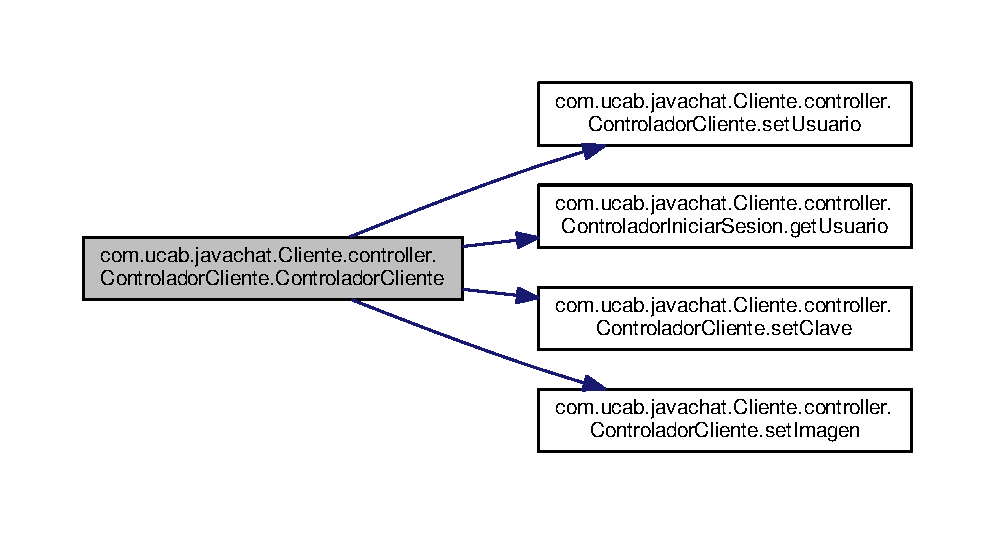
\includegraphics[width=350pt]{d7/d25/classcom_1_1ucab_1_1javachat_1_1_cliente_1_1controller_1_1_controlador_cliente_a169ce22e78795bc739fde02d29afbf5a_cgraph}
\end{center}
\end{figure}




\subsection{Documentación de las funciones miembro}
\hypertarget{classcom_1_1ucab_1_1javachat_1_1_cliente_1_1controller_1_1_controlador_cliente_a132f8481c0894cdad40225f8541931a0}{\index{com\-::ucab\-::javachat\-::\-Cliente\-::controller\-::\-Controlador\-Cliente@{com\-::ucab\-::javachat\-::\-Cliente\-::controller\-::\-Controlador\-Cliente}!action\-Performed@{action\-Performed}}
\index{action\-Performed@{action\-Performed}!com::ucab::javachat::Cliente::controller::ControladorCliente@{com\-::ucab\-::javachat\-::\-Cliente\-::controller\-::\-Controlador\-Cliente}}
\subsubsection[{action\-Performed}]{\setlength{\rightskip}{0pt plus 5cm}final void com.\-ucab.\-javachat.\-Cliente.\-controller.\-Controlador\-Cliente.\-action\-Performed (
\begin{DoxyParamCaption}
\item[{final Action\-Event}]{evt}
\end{DoxyParamCaption}
)}}\label{classcom_1_1ucab_1_1javachat_1_1_cliente_1_1controller_1_1_controlador_cliente_a132f8481c0894cdad40225f8541931a0}
Controlador de eventos al presionar los botones de la ventana 

Definición en la línea 217 del archivo Controlador\-Cliente.\-java.

\hypertarget{classcom_1_1ucab_1_1javachat_1_1_cliente_1_1controller_1_1_controlador_cliente_a3aff80775389cf97755cd5c7db915603}{\index{com\-::ucab\-::javachat\-::\-Cliente\-::controller\-::\-Controlador\-Cliente@{com\-::ucab\-::javachat\-::\-Cliente\-::controller\-::\-Controlador\-Cliente}!agregar\-User@{agregar\-User}}
\index{agregar\-User@{agregar\-User}!com::ucab::javachat::Cliente::controller::ControladorCliente@{com\-::ucab\-::javachat\-::\-Cliente\-::controller\-::\-Controlador\-Cliente}}
\subsubsection[{agregar\-User}]{\setlength{\rightskip}{0pt plus 5cm}final void com.\-ucab.\-javachat.\-Cliente.\-controller.\-Controlador\-Cliente.\-agregar\-User (
\begin{DoxyParamCaption}
\item[{final String}]{user}
\end{DoxyParamCaption}
)}}\label{classcom_1_1ucab_1_1javachat_1_1_cliente_1_1controller_1_1_controlador_cliente_a3aff80775389cf97755cd5c7db915603}
Añade el nombre de usuario del cliente a la lista de usuarios conectados. 
\begin{DoxyParams}{Parámetros}
{\em user} & -\/ N\-Ombre de usuario del cliente. \\
\hline
\end{DoxyParams}


Definición en la línea 180 del archivo Controlador\-Cliente.\-java.

\hypertarget{classcom_1_1ucab_1_1javachat_1_1_cliente_1_1controller_1_1_controlador_cliente_a3e147fa15044b926e8f496e15153e8f9}{\index{com\-::ucab\-::javachat\-::\-Cliente\-::controller\-::\-Controlador\-Cliente@{com\-::ucab\-::javachat\-::\-Cliente\-::controller\-::\-Controlador\-Cliente}!get\-Clave@{get\-Clave}}
\index{get\-Clave@{get\-Clave}!com::ucab::javachat::Cliente::controller::ControladorCliente@{com\-::ucab\-::javachat\-::\-Cliente\-::controller\-::\-Controlador\-Cliente}}
\subsubsection[{get\-Clave}]{\setlength{\rightskip}{0pt plus 5cm}final String com.\-ucab.\-javachat.\-Cliente.\-controller.\-Controlador\-Cliente.\-get\-Clave (
\begin{DoxyParamCaption}
{}
\end{DoxyParamCaption}
)}}\label{classcom_1_1ucab_1_1javachat_1_1_cliente_1_1controller_1_1_controlador_cliente_a3e147fa15044b926e8f496e15153e8f9}
\begin{DoxyReturn}{Devuelve}
La contraseña del usuario que inicio sesion. 
\end{DoxyReturn}


Definición en la línea 131 del archivo Controlador\-Cliente.\-java.

\hypertarget{classcom_1_1ucab_1_1javachat_1_1_cliente_1_1controller_1_1_controlador_cliente_adb75ed57c31baca876b69990bbafb400}{\index{com\-::ucab\-::javachat\-::\-Cliente\-::controller\-::\-Controlador\-Cliente@{com\-::ucab\-::javachat\-::\-Cliente\-::controller\-::\-Controlador\-Cliente}!get\-Imagen@{get\-Imagen}}
\index{get\-Imagen@{get\-Imagen}!com::ucab::javachat::Cliente::controller::ControladorCliente@{com\-::ucab\-::javachat\-::\-Cliente\-::controller\-::\-Controlador\-Cliente}}
\subsubsection[{get\-Imagen}]{\setlength{\rightskip}{0pt plus 5cm}final File com.\-ucab.\-javachat.\-Cliente.\-controller.\-Controlador\-Cliente.\-get\-Imagen (
\begin{DoxyParamCaption}
{}
\end{DoxyParamCaption}
)}}\label{classcom_1_1ucab_1_1javachat_1_1_cliente_1_1controller_1_1_controlador_cliente_adb75ed57c31baca876b69990bbafb400}
\begin{DoxyReturn}{Devuelve}
La imagen del usuario que incio sesion. 
\end{DoxyReturn}


Definición en la línea 148 del archivo Controlador\-Cliente.\-java.

\hypertarget{classcom_1_1ucab_1_1javachat_1_1_cliente_1_1controller_1_1_controlador_cliente_ada03c074086d0d54321cdf0347147397}{\index{com\-::ucab\-::javachat\-::\-Cliente\-::controller\-::\-Controlador\-Cliente@{com\-::ucab\-::javachat\-::\-Cliente\-::controller\-::\-Controlador\-Cliente}!get\-Usuario@{get\-Usuario}}
\index{get\-Usuario@{get\-Usuario}!com::ucab::javachat::Cliente::controller::ControladorCliente@{com\-::ucab\-::javachat\-::\-Cliente\-::controller\-::\-Controlador\-Cliente}}
\subsubsection[{get\-Usuario}]{\setlength{\rightskip}{0pt plus 5cm}final String com.\-ucab.\-javachat.\-Cliente.\-controller.\-Controlador\-Cliente.\-get\-Usuario (
\begin{DoxyParamCaption}
{}
\end{DoxyParamCaption}
)}}\label{classcom_1_1ucab_1_1javachat_1_1_cliente_1_1controller_1_1_controlador_cliente_ada03c074086d0d54321cdf0347147397}
\begin{DoxyReturn}{Devuelve}
El nombre del usuario que inicio sesion. 
\end{DoxyReturn}


Definición en la línea 115 del archivo Controlador\-Cliente.\-java.



Gráfico de llamadas a esta función\-:
\nopagebreak
\begin{figure}[H]
\begin{center}
\leavevmode
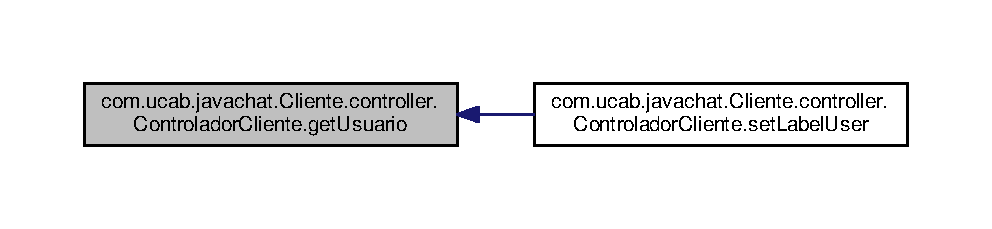
\includegraphics[width=350pt]{d7/d25/classcom_1_1ucab_1_1javachat_1_1_cliente_1_1controller_1_1_controlador_cliente_ada03c074086d0d54321cdf0347147397_icgraph}
\end{center}
\end{figure}


\hypertarget{classcom_1_1ucab_1_1javachat_1_1_cliente_1_1controller_1_1_controlador_cliente_a0ec86bb408cc78782346b4c01b95a7d6}{\index{com\-::ucab\-::javachat\-::\-Cliente\-::controller\-::\-Controlador\-Cliente@{com\-::ucab\-::javachat\-::\-Cliente\-::controller\-::\-Controlador\-Cliente}!poner\-Activos@{poner\-Activos}}
\index{poner\-Activos@{poner\-Activos}!com::ucab::javachat::Cliente::controller::ControladorCliente@{com\-::ucab\-::javachat\-::\-Cliente\-::controller\-::\-Controlador\-Cliente}}
\subsubsection[{poner\-Activos}]{\setlength{\rightskip}{0pt plus 5cm}final void com.\-ucab.\-javachat.\-Cliente.\-controller.\-Controlador\-Cliente.\-poner\-Activos (
\begin{DoxyParamCaption}
\item[{final Vector$<$ String $>$}]{datos}
\end{DoxyParamCaption}
)}}\label{classcom_1_1ucab_1_1javachat_1_1_cliente_1_1controller_1_1_controlador_cliente_a0ec86bb408cc78782346b4c01b95a7d6}
Muestra en la ventana la lista de usuarios conectados. 
\begin{DoxyParams}{Parámetros}
{\em datos} & -\/ Vector que contiene los nombres de los usuarios conectados. \\
\hline
\end{DoxyParams}


Definición en la línea 171 del archivo Controlador\-Cliente.\-java.

\hypertarget{classcom_1_1ucab_1_1javachat_1_1_cliente_1_1controller_1_1_controlador_cliente_abb244f9e8904743e123c5e86a42c4710}{\index{com\-::ucab\-::javachat\-::\-Cliente\-::controller\-::\-Controlador\-Cliente@{com\-::ucab\-::javachat\-::\-Cliente\-::controller\-::\-Controlador\-Cliente}!retirra\-User@{retirra\-User}}
\index{retirra\-User@{retirra\-User}!com::ucab::javachat::Cliente::controller::ControladorCliente@{com\-::ucab\-::javachat\-::\-Cliente\-::controller\-::\-Controlador\-Cliente}}
\subsubsection[{retirra\-User}]{\setlength{\rightskip}{0pt plus 5cm}final void com.\-ucab.\-javachat.\-Cliente.\-controller.\-Controlador\-Cliente.\-retirra\-User (
\begin{DoxyParamCaption}
\item[{final String}]{user}
\end{DoxyParamCaption}
)}}\label{classcom_1_1ucab_1_1javachat_1_1_cliente_1_1controller_1_1_controlador_cliente_abb244f9e8904743e123c5e86a42c4710}
retira el nombre de usuario del cliente. P\-D\-: E\-S\-T\-E M\-E\-T\-O\-D\-O N\-U\-N\-C\-A S\-E U\-S\-A. 
\begin{DoxyParams}{Parámetros}
{\em user} & \\
\hline
\end{DoxyParams}


Definición en la línea 190 del archivo Controlador\-Cliente.\-java.

\hypertarget{classcom_1_1ucab_1_1javachat_1_1_cliente_1_1controller_1_1_controlador_cliente_a8647e56fdb735f7abdef284b023e9f53}{\index{com\-::ucab\-::javachat\-::\-Cliente\-::controller\-::\-Controlador\-Cliente@{com\-::ucab\-::javachat\-::\-Cliente\-::controller\-::\-Controlador\-Cliente}!set\-Clave@{set\-Clave}}
\index{set\-Clave@{set\-Clave}!com::ucab::javachat::Cliente::controller::ControladorCliente@{com\-::ucab\-::javachat\-::\-Cliente\-::controller\-::\-Controlador\-Cliente}}
\subsubsection[{set\-Clave}]{\setlength{\rightskip}{0pt plus 5cm}final void com.\-ucab.\-javachat.\-Cliente.\-controller.\-Controlador\-Cliente.\-set\-Clave (
\begin{DoxyParamCaption}
\item[{final String}]{clave}
\end{DoxyParamCaption}
)}}\label{classcom_1_1ucab_1_1javachat_1_1_cliente_1_1controller_1_1_controlador_cliente_a8647e56fdb735f7abdef284b023e9f53}
Guarda la contraseña del usuario que quiere iniciar sesion. 
\begin{DoxyParams}{Parámetros}
{\em clave} & \\
\hline
\end{DoxyParams}


Definición en la línea 140 del archivo Controlador\-Cliente.\-java.



Gráfico de llamadas a esta función\-:
\nopagebreak
\begin{figure}[H]
\begin{center}
\leavevmode
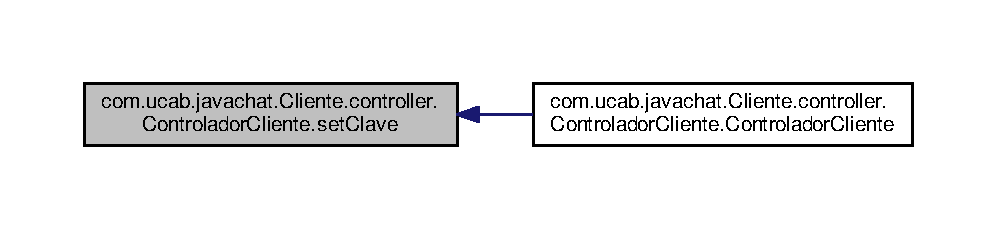
\includegraphics[width=350pt]{d7/d25/classcom_1_1ucab_1_1javachat_1_1_cliente_1_1controller_1_1_controlador_cliente_a8647e56fdb735f7abdef284b023e9f53_icgraph}
\end{center}
\end{figure}


\hypertarget{classcom_1_1ucab_1_1javachat_1_1_cliente_1_1controller_1_1_controlador_cliente_a6e7b9e6c4a82829efbd0aae6c2658184}{\index{com\-::ucab\-::javachat\-::\-Cliente\-::controller\-::\-Controlador\-Cliente@{com\-::ucab\-::javachat\-::\-Cliente\-::controller\-::\-Controlador\-Cliente}!set\-Imagen@{set\-Imagen}}
\index{set\-Imagen@{set\-Imagen}!com::ucab::javachat::Cliente::controller::ControladorCliente@{com\-::ucab\-::javachat\-::\-Cliente\-::controller\-::\-Controlador\-Cliente}}
\subsubsection[{set\-Imagen}]{\setlength{\rightskip}{0pt plus 5cm}final void com.\-ucab.\-javachat.\-Cliente.\-controller.\-Controlador\-Cliente.\-set\-Imagen (
\begin{DoxyParamCaption}
\item[{final File}]{imagen}
\end{DoxyParamCaption}
)}}\label{classcom_1_1ucab_1_1javachat_1_1_cliente_1_1controller_1_1_controlador_cliente_a6e7b9e6c4a82829efbd0aae6c2658184}
Guarda la imagen del usuario que quiere iniciar sesion. 
\begin{DoxyParams}{Parámetros}
{\em imagen} & \\
\hline
\end{DoxyParams}


Definición en la línea 156 del archivo Controlador\-Cliente.\-java.



Gráfico de llamadas a esta función\-:
\nopagebreak
\begin{figure}[H]
\begin{center}
\leavevmode
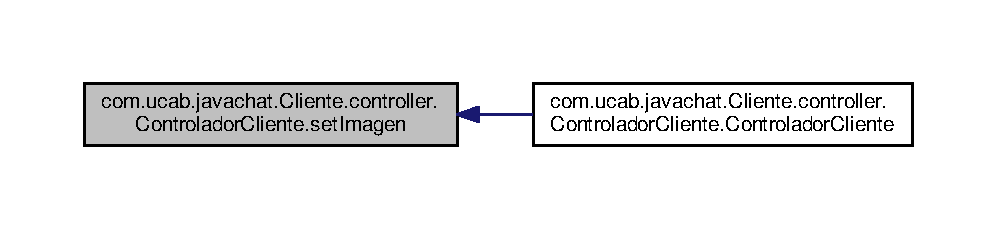
\includegraphics[width=350pt]{d7/d25/classcom_1_1ucab_1_1javachat_1_1_cliente_1_1controller_1_1_controlador_cliente_a6e7b9e6c4a82829efbd0aae6c2658184_icgraph}
\end{center}
\end{figure}


\hypertarget{classcom_1_1ucab_1_1javachat_1_1_cliente_1_1controller_1_1_controlador_cliente_aa19a69efd4f74891f467345498ddcb39}{\index{com\-::ucab\-::javachat\-::\-Cliente\-::controller\-::\-Controlador\-Cliente@{com\-::ucab\-::javachat\-::\-Cliente\-::controller\-::\-Controlador\-Cliente}!set\-Label\-User@{set\-Label\-User}}
\index{set\-Label\-User@{set\-Label\-User}!com::ucab::javachat::Cliente::controller::ControladorCliente@{com\-::ucab\-::javachat\-::\-Cliente\-::controller\-::\-Controlador\-Cliente}}
\subsubsection[{set\-Label\-User}]{\setlength{\rightskip}{0pt plus 5cm}final void com.\-ucab.\-javachat.\-Cliente.\-controller.\-Controlador\-Cliente.\-set\-Label\-User (
\begin{DoxyParamCaption}
{}
\end{DoxyParamCaption}
)}}\label{classcom_1_1ucab_1_1javachat_1_1_cliente_1_1controller_1_1_controlador_cliente_aa19a69efd4f74891f467345498ddcb39}
Muestra en la ventana el nombre de usuario del cliente. 

Definición en la línea 163 del archivo Controlador\-Cliente.\-java.



Gráfico de llamadas para esta función\-:
\nopagebreak
\begin{figure}[H]
\begin{center}
\leavevmode
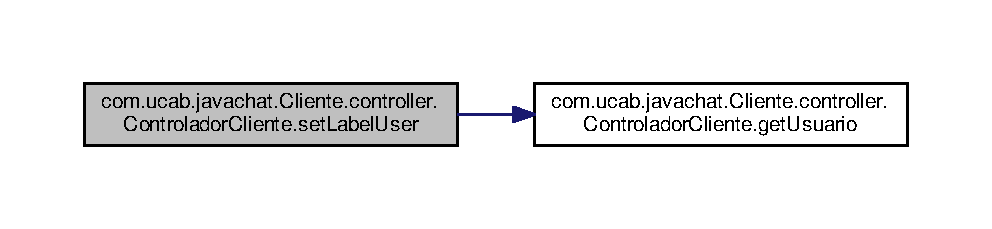
\includegraphics[width=350pt]{d7/d25/classcom_1_1ucab_1_1javachat_1_1_cliente_1_1controller_1_1_controlador_cliente_aa19a69efd4f74891f467345498ddcb39_cgraph}
\end{center}
\end{figure}


\hypertarget{classcom_1_1ucab_1_1javachat_1_1_cliente_1_1controller_1_1_controlador_cliente_a29e6cb2c38d42517282ce2da900b3516}{\index{com\-::ucab\-::javachat\-::\-Cliente\-::controller\-::\-Controlador\-Cliente@{com\-::ucab\-::javachat\-::\-Cliente\-::controller\-::\-Controlador\-Cliente}!set\-Usuario@{set\-Usuario}}
\index{set\-Usuario@{set\-Usuario}!com::ucab::javachat::Cliente::controller::ControladorCliente@{com\-::ucab\-::javachat\-::\-Cliente\-::controller\-::\-Controlador\-Cliente}}
\subsubsection[{set\-Usuario}]{\setlength{\rightskip}{0pt plus 5cm}final void com.\-ucab.\-javachat.\-Cliente.\-controller.\-Controlador\-Cliente.\-set\-Usuario (
\begin{DoxyParamCaption}
\item[{final String}]{usuario}
\end{DoxyParamCaption}
)}}\label{classcom_1_1ucab_1_1javachat_1_1_cliente_1_1controller_1_1_controlador_cliente_a29e6cb2c38d42517282ce2da900b3516}
Guarda el nombre del usuario que quiere iniciar sesion. 
\begin{DoxyParams}{Parámetros}
{\em user} & -\/ Nombre de usuario. \\
\hline
\end{DoxyParams}


Definición en la línea 123 del archivo Controlador\-Cliente.\-java.



Gráfico de llamadas a esta función\-:
\nopagebreak
\begin{figure}[H]
\begin{center}
\leavevmode
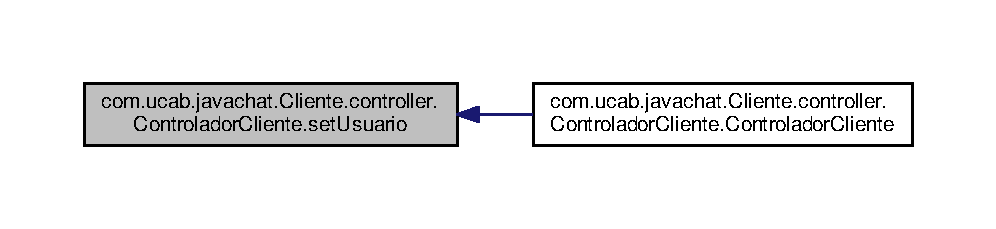
\includegraphics[width=350pt]{d7/d25/classcom_1_1ucab_1_1javachat_1_1_cliente_1_1controller_1_1_controlador_cliente_a29e6cb2c38d42517282ce2da900b3516_icgraph}
\end{center}
\end{figure}




La documentación para esta clase fue generada a partir del siguiente fichero\-:\begin{DoxyCompactItemize}
\item 
Chat-\/\-Codigo-\/\-Morse/\-Chat\-Morse/src/com/ucab/javachat/\-Cliente/controller/Controlador\-Cliente.\-java\end{DoxyCompactItemize}

\hypertarget{classcom_1_1ucab_1_1javachat_1_1_cliente_1_1controller_1_1_controlador_iniciar_sesion}{\section{Referencia de la Clase com.\-ucab.\-javachat.\-Cliente.\-controller.\-Controlador\-Iniciar\-Sesion}
\label{classcom_1_1ucab_1_1javachat_1_1_cliente_1_1controller_1_1_controlador_iniciar_sesion}\index{com.\-ucab.\-javachat.\-Cliente.\-controller.\-Controlador\-Iniciar\-Sesion@{com.\-ucab.\-javachat.\-Cliente.\-controller.\-Controlador\-Iniciar\-Sesion}}
}


Diagrama de herencias de com.\-ucab.\-javachat.\-Cliente.\-controller.\-Controlador\-Iniciar\-Sesion
\nopagebreak
\begin{figure}[H]
\begin{center}
\leavevmode
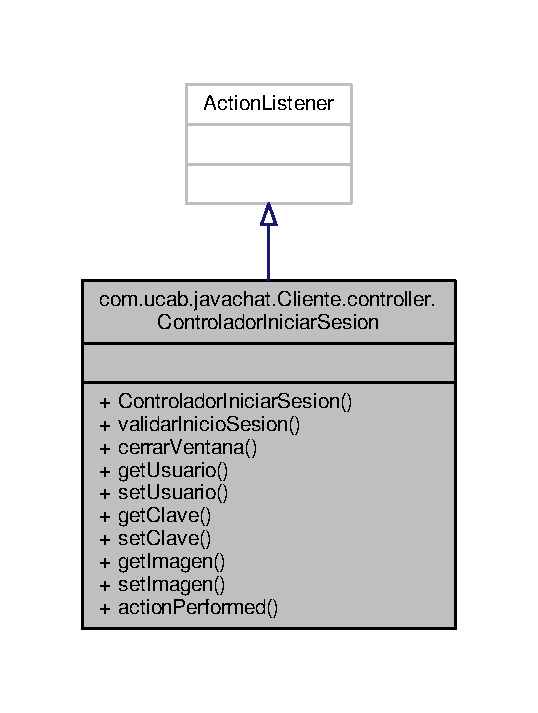
\includegraphics[width=258pt]{d1/d5f/classcom_1_1ucab_1_1javachat_1_1_cliente_1_1controller_1_1_controlador_iniciar_sesion__inherit__graph}
\end{center}
\end{figure}


Diagrama de colaboración para com.\-ucab.\-javachat.\-Cliente.\-controller.\-Controlador\-Iniciar\-Sesion\-:
\nopagebreak
\begin{figure}[H]
\begin{center}
\leavevmode
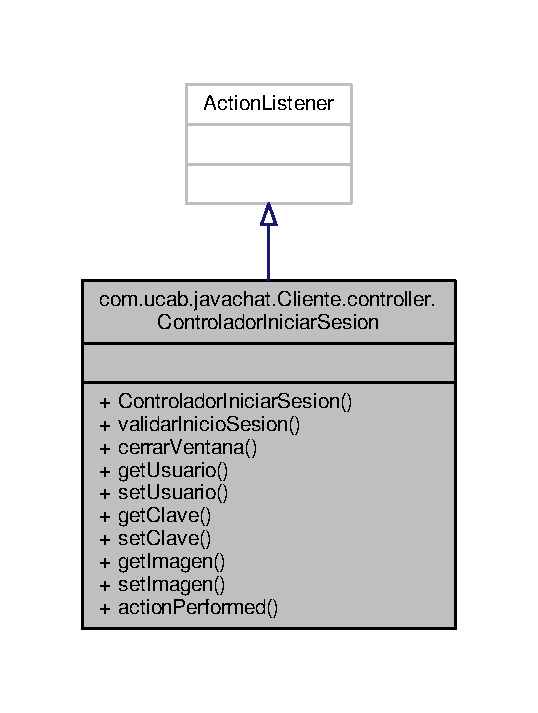
\includegraphics[width=258pt]{db/d9c/classcom_1_1ucab_1_1javachat_1_1_cliente_1_1controller_1_1_controlador_iniciar_sesion__coll__graph}
\end{center}
\end{figure}
\subsection*{Métodos públicos}
\begin{DoxyCompactItemize}
\item 
\hypertarget{classcom_1_1ucab_1_1javachat_1_1_cliente_1_1controller_1_1_controlador_iniciar_sesion_ac0ae95fb81e6a3282769c3a48d99340f}{{\bfseries Controlador\-Iniciar\-Sesion} (final \hyperlink{classcom_1_1ucab_1_1javachat_1_1_cliente_1_1view_1_1_vent_iniciar_sesion}{Vent\-Iniciar\-Sesion} vista)}\label{classcom_1_1ucab_1_1javachat_1_1_cliente_1_1controller_1_1_controlador_iniciar_sesion_ac0ae95fb81e6a3282769c3a48d99340f}

\item 
final boolean \hyperlink{classcom_1_1ucab_1_1javachat_1_1_cliente_1_1controller_1_1_controlador_iniciar_sesion_a0af254dfeeb830b945c72b3f918c4145}{validar\-Inicio\-Sesion} ()
\item 
\hypertarget{classcom_1_1ucab_1_1javachat_1_1_cliente_1_1controller_1_1_controlador_iniciar_sesion_a3f847e72a97f9af00ae6013eb073a8e2}{void {\bfseries cerrar\-Ventana} ()}\label{classcom_1_1ucab_1_1javachat_1_1_cliente_1_1controller_1_1_controlador_iniciar_sesion_a3f847e72a97f9af00ae6013eb073a8e2}

\item 
String \hyperlink{classcom_1_1ucab_1_1javachat_1_1_cliente_1_1controller_1_1_controlador_iniciar_sesion_ad4d15c39f79ab5c60375ad42fbca1b01}{get\-Usuario} ()
\item 
\hypertarget{classcom_1_1ucab_1_1javachat_1_1_cliente_1_1controller_1_1_controlador_iniciar_sesion_a93241d6ec2f9d3f2ed60c936d7bcffab}{void {\bfseries set\-Usuario} (String usuario)}\label{classcom_1_1ucab_1_1javachat_1_1_cliente_1_1controller_1_1_controlador_iniciar_sesion_a93241d6ec2f9d3f2ed60c936d7bcffab}

\item 
\hypertarget{classcom_1_1ucab_1_1javachat_1_1_cliente_1_1controller_1_1_controlador_iniciar_sesion_a9b1fd5a6d9813bc1f32041210a50876a}{String {\bfseries get\-Clave} ()}\label{classcom_1_1ucab_1_1javachat_1_1_cliente_1_1controller_1_1_controlador_iniciar_sesion_a9b1fd5a6d9813bc1f32041210a50876a}

\item 
\hypertarget{classcom_1_1ucab_1_1javachat_1_1_cliente_1_1controller_1_1_controlador_iniciar_sesion_a9cf2679039366d1f9e37d2d506dec14c}{void {\bfseries set\-Clave} (String clave)}\label{classcom_1_1ucab_1_1javachat_1_1_cliente_1_1controller_1_1_controlador_iniciar_sesion_a9cf2679039366d1f9e37d2d506dec14c}

\item 
\hypertarget{classcom_1_1ucab_1_1javachat_1_1_cliente_1_1controller_1_1_controlador_iniciar_sesion_a5e8b49d814d3693a88e5e431155bb830}{File {\bfseries get\-Imagen} ()}\label{classcom_1_1ucab_1_1javachat_1_1_cliente_1_1controller_1_1_controlador_iniciar_sesion_a5e8b49d814d3693a88e5e431155bb830}

\item 
\hypertarget{classcom_1_1ucab_1_1javachat_1_1_cliente_1_1controller_1_1_controlador_iniciar_sesion_abb99292844ba8b9f1e7379ec01ab9d93}{void {\bfseries set\-Imagen} (File imagen)}\label{classcom_1_1ucab_1_1javachat_1_1_cliente_1_1controller_1_1_controlador_iniciar_sesion_abb99292844ba8b9f1e7379ec01ab9d93}

\item 
void \hyperlink{classcom_1_1ucab_1_1javachat_1_1_cliente_1_1controller_1_1_controlador_iniciar_sesion_a3b51bc4dfb6429cb3d98387b57fc19f3}{action\-Performed} (Action\-Event e)
\end{DoxyCompactItemize}


\subsection{Descripción detallada}
Clase del controlador para la ventana de inicio de sesion \begin{DoxyAuthor}{Autores}
Grupo 3 
\end{DoxyAuthor}


Definición en la línea 21 del archivo Controlador\-Iniciar\-Sesion.\-java.



\subsection{Documentación de las funciones miembro}
\hypertarget{classcom_1_1ucab_1_1javachat_1_1_cliente_1_1controller_1_1_controlador_iniciar_sesion_a3b51bc4dfb6429cb3d98387b57fc19f3}{\index{com\-::ucab\-::javachat\-::\-Cliente\-::controller\-::\-Controlador\-Iniciar\-Sesion@{com\-::ucab\-::javachat\-::\-Cliente\-::controller\-::\-Controlador\-Iniciar\-Sesion}!action\-Performed@{action\-Performed}}
\index{action\-Performed@{action\-Performed}!com::ucab::javachat::Cliente::controller::ControladorIniciarSesion@{com\-::ucab\-::javachat\-::\-Cliente\-::controller\-::\-Controlador\-Iniciar\-Sesion}}
\subsubsection[{action\-Performed}]{\setlength{\rightskip}{0pt plus 5cm}void com.\-ucab.\-javachat.\-Cliente.\-controller.\-Controlador\-Iniciar\-Sesion.\-action\-Performed (
\begin{DoxyParamCaption}
\item[{Action\-Event}]{e}
\end{DoxyParamCaption}
)}}\label{classcom_1_1ucab_1_1javachat_1_1_cliente_1_1controller_1_1_controlador_iniciar_sesion_a3b51bc4dfb6429cb3d98387b57fc19f3}
metodo encargado de la accion de cada boton en la ventana de inicio de sesion. 

Definición en la línea 107 del archivo Controlador\-Iniciar\-Sesion.\-java.



Gráfico de llamadas para esta función\-:
\nopagebreak
\begin{figure}[H]
\begin{center}
\leavevmode
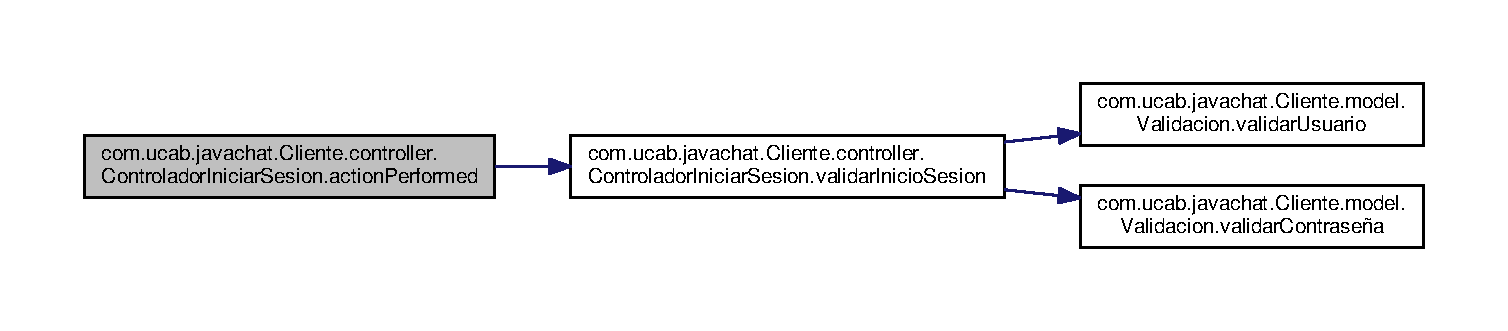
\includegraphics[width=350pt]{d2/d0e/classcom_1_1ucab_1_1javachat_1_1_cliente_1_1controller_1_1_controlador_iniciar_sesion_a3b51bc4dfb6429cb3d98387b57fc19f3_cgraph}
\end{center}
\end{figure}


\hypertarget{classcom_1_1ucab_1_1javachat_1_1_cliente_1_1controller_1_1_controlador_iniciar_sesion_ad4d15c39f79ab5c60375ad42fbca1b01}{\index{com\-::ucab\-::javachat\-::\-Cliente\-::controller\-::\-Controlador\-Iniciar\-Sesion@{com\-::ucab\-::javachat\-::\-Cliente\-::controller\-::\-Controlador\-Iniciar\-Sesion}!get\-Usuario@{get\-Usuario}}
\index{get\-Usuario@{get\-Usuario}!com::ucab::javachat::Cliente::controller::ControladorIniciarSesion@{com\-::ucab\-::javachat\-::\-Cliente\-::controller\-::\-Controlador\-Iniciar\-Sesion}}
\subsubsection[{get\-Usuario}]{\setlength{\rightskip}{0pt plus 5cm}String com.\-ucab.\-javachat.\-Cliente.\-controller.\-Controlador\-Iniciar\-Sesion.\-get\-Usuario (
\begin{DoxyParamCaption}
{}
\end{DoxyParamCaption}
)}}\label{classcom_1_1ucab_1_1javachat_1_1_cliente_1_1controller_1_1_controlador_iniciar_sesion_ad4d15c39f79ab5c60375ad42fbca1b01}
getters y setters \begin{DoxyReturn}{Devuelve}

\end{DoxyReturn}


Definición en la línea 80 del archivo Controlador\-Iniciar\-Sesion.\-java.



Gráfico de llamadas a esta función\-:
\nopagebreak
\begin{figure}[H]
\begin{center}
\leavevmode
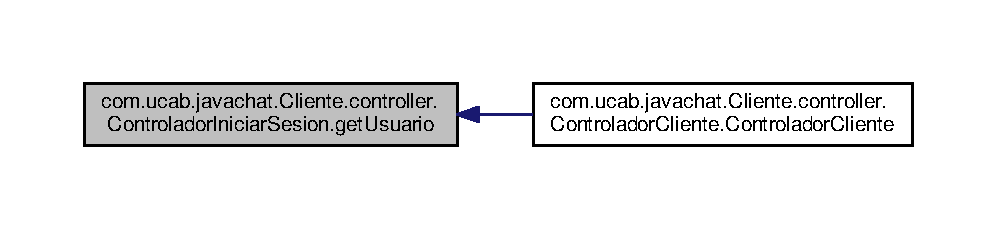
\includegraphics[width=350pt]{d2/d0e/classcom_1_1ucab_1_1javachat_1_1_cliente_1_1controller_1_1_controlador_iniciar_sesion_ad4d15c39f79ab5c60375ad42fbca1b01_icgraph}
\end{center}
\end{figure}


\hypertarget{classcom_1_1ucab_1_1javachat_1_1_cliente_1_1controller_1_1_controlador_iniciar_sesion_a0af254dfeeb830b945c72b3f918c4145}{\index{com\-::ucab\-::javachat\-::\-Cliente\-::controller\-::\-Controlador\-Iniciar\-Sesion@{com\-::ucab\-::javachat\-::\-Cliente\-::controller\-::\-Controlador\-Iniciar\-Sesion}!validar\-Inicio\-Sesion@{validar\-Inicio\-Sesion}}
\index{validar\-Inicio\-Sesion@{validar\-Inicio\-Sesion}!com::ucab::javachat::Cliente::controller::ControladorIniciarSesion@{com\-::ucab\-::javachat\-::\-Cliente\-::controller\-::\-Controlador\-Iniciar\-Sesion}}
\subsubsection[{validar\-Inicio\-Sesion}]{\setlength{\rightskip}{0pt plus 5cm}final boolean com.\-ucab.\-javachat.\-Cliente.\-controller.\-Controlador\-Iniciar\-Sesion.\-validar\-Inicio\-Sesion (
\begin{DoxyParamCaption}
{}
\end{DoxyParamCaption}
)}}\label{classcom_1_1ucab_1_1javachat_1_1_cliente_1_1controller_1_1_controlador_iniciar_sesion_a0af254dfeeb830b945c72b3f918c4145}
Metodo que valida los datos ingresados con el archivo Json de registro. \begin{DoxyReturn}{Devuelve}
boolean flag. Si los datos son correctos el valor devuelto sera verdadero. Si alguno de los datos ingresados no coincide con el archivo de registro el valor devuelto sera falso. 
\end{DoxyReturn}


Definición en la línea 45 del archivo Controlador\-Iniciar\-Sesion.\-java.



Gráfico de llamadas para esta función\-:
\nopagebreak
\begin{figure}[H]
\begin{center}
\leavevmode
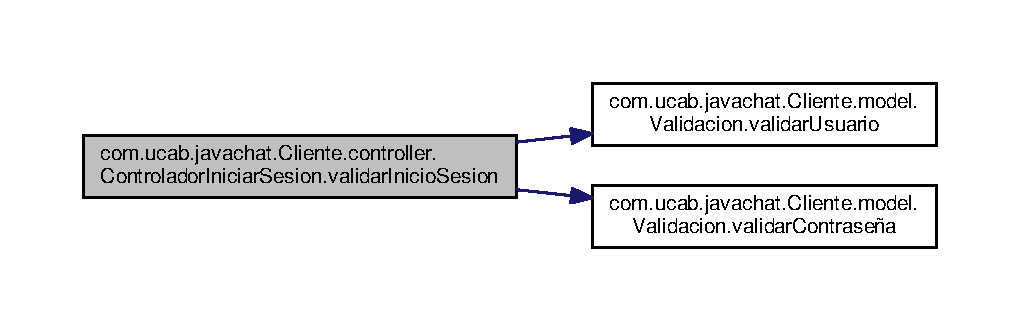
\includegraphics[width=350pt]{d2/d0e/classcom_1_1ucab_1_1javachat_1_1_cliente_1_1controller_1_1_controlador_iniciar_sesion_a0af254dfeeb830b945c72b3f918c4145_cgraph}
\end{center}
\end{figure}




Gráfico de llamadas a esta función\-:
\nopagebreak
\begin{figure}[H]
\begin{center}
\leavevmode
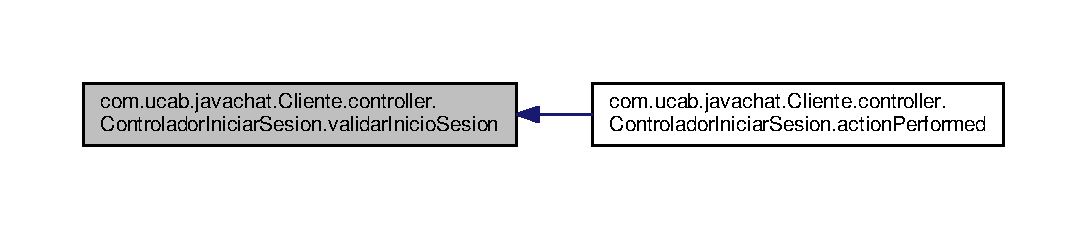
\includegraphics[width=350pt]{d2/d0e/classcom_1_1ucab_1_1javachat_1_1_cliente_1_1controller_1_1_controlador_iniciar_sesion_a0af254dfeeb830b945c72b3f918c4145_icgraph}
\end{center}
\end{figure}




La documentación para esta clase fue generada a partir del siguiente fichero\-:\begin{DoxyCompactItemize}
\item 
Chat-\/\-Codigo-\/\-Morse/\-Chat\-Morse/src/com/ucab/javachat/\-Cliente/controller/Controlador\-Iniciar\-Sesion.\-java\end{DoxyCompactItemize}

\hypertarget{classcom_1_1ucab_1_1javachat_1_1_cliente_1_1controller_1_1_controlador_modificar}{\section{Referencia de la Clase com.\-ucab.\-javachat.\-Cliente.\-controller.\-Controlador\-Modificar}
\label{classcom_1_1ucab_1_1javachat_1_1_cliente_1_1controller_1_1_controlador_modificar}\index{com.\-ucab.\-javachat.\-Cliente.\-controller.\-Controlador\-Modificar@{com.\-ucab.\-javachat.\-Cliente.\-controller.\-Controlador\-Modificar}}
}


Diagrama de herencias de com.\-ucab.\-javachat.\-Cliente.\-controller.\-Controlador\-Modificar
\nopagebreak
\begin{figure}[H]
\begin{center}
\leavevmode
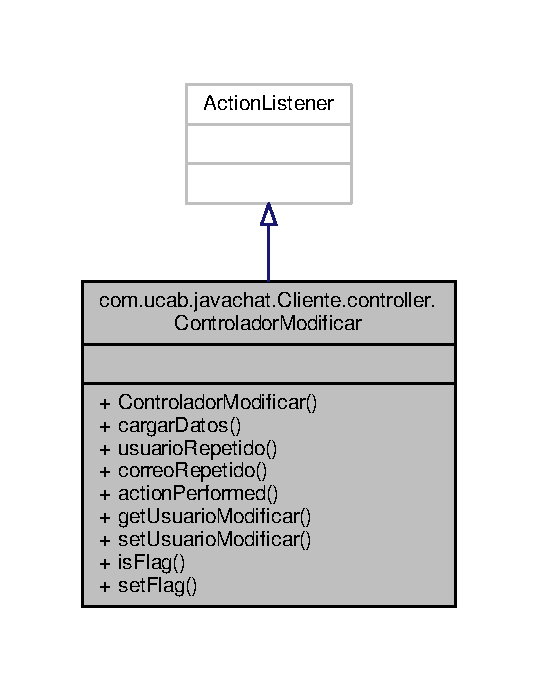
\includegraphics[width=258pt]{d7/dcb/classcom_1_1ucab_1_1javachat_1_1_cliente_1_1controller_1_1_controlador_modificar__inherit__graph}
\end{center}
\end{figure}


Diagrama de colaboración para com.\-ucab.\-javachat.\-Cliente.\-controller.\-Controlador\-Modificar\-:
\nopagebreak
\begin{figure}[H]
\begin{center}
\leavevmode
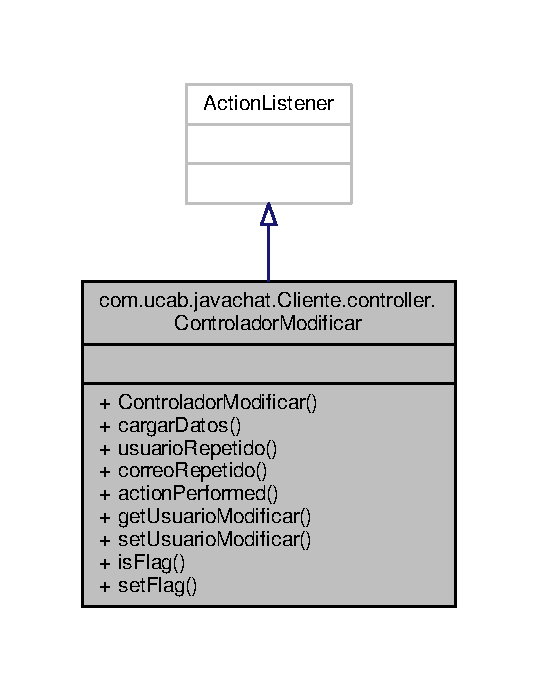
\includegraphics[width=258pt]{dc/d5d/classcom_1_1ucab_1_1javachat_1_1_cliente_1_1controller_1_1_controlador_modificar__coll__graph}
\end{center}
\end{figure}
\subsection*{Métodos públicos}
\begin{DoxyCompactItemize}
\item 
\hypertarget{classcom_1_1ucab_1_1javachat_1_1_cliente_1_1controller_1_1_controlador_modificar_a6123a8b8e53bbf04d1a68ff4722e2dd9}{{\bfseries Controlador\-Modificar} (final \hyperlink{classcom_1_1ucab_1_1javachat_1_1_cliente_1_1view_1_1_vent_modificar}{Vent\-Modificar} vista, \hyperlink{classcom_1_1ucab_1_1javachat_1_1_cliente_1_1model_1_1_cliente}{Cliente} cliente)}\label{classcom_1_1ucab_1_1javachat_1_1_cliente_1_1controller_1_1_controlador_modificar_a6123a8b8e53bbf04d1a68ff4722e2dd9}

\item 
final void \hyperlink{classcom_1_1ucab_1_1javachat_1_1_cliente_1_1controller_1_1_controlador_modificar_a70d237e77c3b71f36bbacf7273ecc928}{cargar\-Datos} (final \hyperlink{classcom_1_1ucab_1_1javachat_1_1_cliente_1_1model_1_1_usuario}{Usuario} modelo)
\item 
final void \hyperlink{classcom_1_1ucab_1_1javachat_1_1_cliente_1_1controller_1_1_controlador_modificar_a98998ef15a60c2652086c638f3d49626}{usuario\-Repetido} ()
\item 
final void \hyperlink{classcom_1_1ucab_1_1javachat_1_1_cliente_1_1controller_1_1_controlador_modificar_a15be7ce5dba7613ab67666421ad5df8b}{correo\-Repetido} ()
\item 
final void \hyperlink{classcom_1_1ucab_1_1javachat_1_1_cliente_1_1controller_1_1_controlador_modificar_adf78b1559924c21769b55b0c3f5d799f}{action\-Performed} (final Action\-Event evento)
\item 
final \hyperlink{classcom_1_1ucab_1_1javachat_1_1_cliente_1_1model_1_1_usuario}{Usuario} \hyperlink{classcom_1_1ucab_1_1javachat_1_1_cliente_1_1controller_1_1_controlador_modificar_a50fed3d5d044639f7a4d8fc076876d88}{get\-Usuario\-Modificar} ()
\item 
\hypertarget{classcom_1_1ucab_1_1javachat_1_1_cliente_1_1controller_1_1_controlador_modificar_a567c65f9fbdc43f40e4ab0dd7c047ba9}{final void {\bfseries set\-Usuario\-Modificar} (final \hyperlink{classcom_1_1ucab_1_1javachat_1_1_cliente_1_1model_1_1_usuario}{Usuario} usuario\-Modificar)}\label{classcom_1_1ucab_1_1javachat_1_1_cliente_1_1controller_1_1_controlador_modificar_a567c65f9fbdc43f40e4ab0dd7c047ba9}

\item 
\hypertarget{classcom_1_1ucab_1_1javachat_1_1_cliente_1_1controller_1_1_controlador_modificar_a8a658d9065bd5f1e88a2a99f23d50784}{final boolean {\bfseries is\-Flag} ()}\label{classcom_1_1ucab_1_1javachat_1_1_cliente_1_1controller_1_1_controlador_modificar_a8a658d9065bd5f1e88a2a99f23d50784}

\item 
\hypertarget{classcom_1_1ucab_1_1javachat_1_1_cliente_1_1controller_1_1_controlador_modificar_ade1618d2df8cbec7a97be5c2ee1d3eca}{final void {\bfseries set\-Flag} (final boolean flag)}\label{classcom_1_1ucab_1_1javachat_1_1_cliente_1_1controller_1_1_controlador_modificar_ade1618d2df8cbec7a97be5c2ee1d3eca}

\end{DoxyCompactItemize}


\subsection{Descripción detallada}
Clase encargada de la ventana que se muestra cuando se desean hacer cambios en la informacion de un usuario. \begin{DoxyAuthor}{Autor}
Grupo 3 -\/ A. Rodriguez, I. Teixeira, L. Valladares, D. Suarez 
\end{DoxyAuthor}


Definición en la línea 24 del archivo Controlador\-Modificar.\-java.



\subsection{Documentación de las funciones miembro}
\hypertarget{classcom_1_1ucab_1_1javachat_1_1_cliente_1_1controller_1_1_controlador_modificar_adf78b1559924c21769b55b0c3f5d799f}{\index{com\-::ucab\-::javachat\-::\-Cliente\-::controller\-::\-Controlador\-Modificar@{com\-::ucab\-::javachat\-::\-Cliente\-::controller\-::\-Controlador\-Modificar}!action\-Performed@{action\-Performed}}
\index{action\-Performed@{action\-Performed}!com::ucab::javachat::Cliente::controller::ControladorModificar@{com\-::ucab\-::javachat\-::\-Cliente\-::controller\-::\-Controlador\-Modificar}}
\subsubsection[{action\-Performed}]{\setlength{\rightskip}{0pt plus 5cm}final void com.\-ucab.\-javachat.\-Cliente.\-controller.\-Controlador\-Modificar.\-action\-Performed (
\begin{DoxyParamCaption}
\item[{final Action\-Event}]{evento}
\end{DoxyParamCaption}
)}}\label{classcom_1_1ucab_1_1javachat_1_1_cliente_1_1controller_1_1_controlador_modificar_adf78b1559924c21769b55b0c3f5d799f}
metodo encargado de la accion de los botones y campos de textos en la ventana que se muestra 

Definición en la línea 78 del archivo Controlador\-Modificar.\-java.



Gráfico de llamadas para esta función\-:
\nopagebreak
\begin{figure}[H]
\begin{center}
\leavevmode
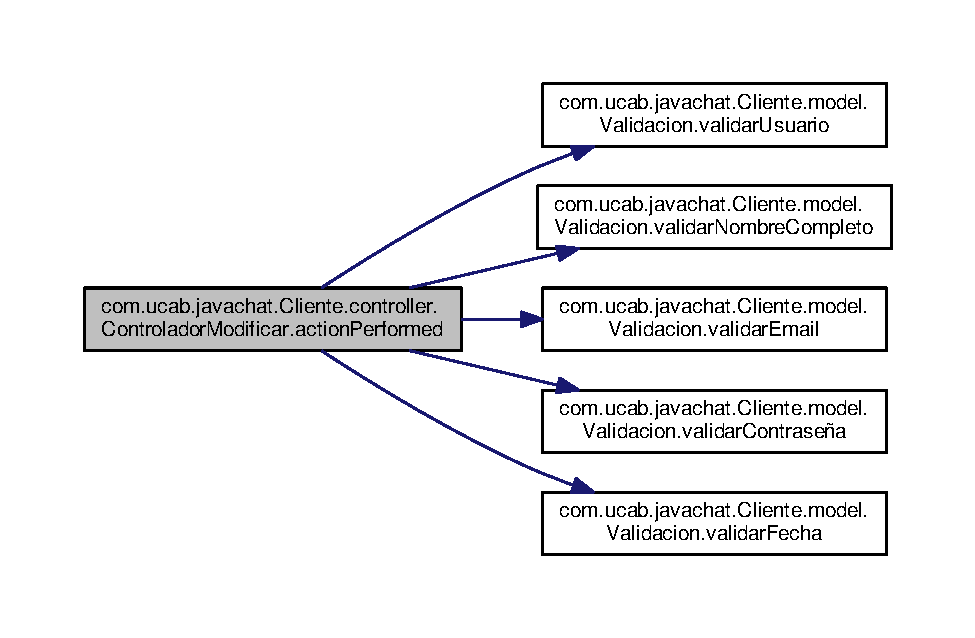
\includegraphics[width=350pt]{d6/d90/classcom_1_1ucab_1_1javachat_1_1_cliente_1_1controller_1_1_controlador_modificar_adf78b1559924c21769b55b0c3f5d799f_cgraph}
\end{center}
\end{figure}


\hypertarget{classcom_1_1ucab_1_1javachat_1_1_cliente_1_1controller_1_1_controlador_modificar_a70d237e77c3b71f36bbacf7273ecc928}{\index{com\-::ucab\-::javachat\-::\-Cliente\-::controller\-::\-Controlador\-Modificar@{com\-::ucab\-::javachat\-::\-Cliente\-::controller\-::\-Controlador\-Modificar}!cargar\-Datos@{cargar\-Datos}}
\index{cargar\-Datos@{cargar\-Datos}!com::ucab::javachat::Cliente::controller::ControladorModificar@{com\-::ucab\-::javachat\-::\-Cliente\-::controller\-::\-Controlador\-Modificar}}
\subsubsection[{cargar\-Datos}]{\setlength{\rightskip}{0pt plus 5cm}final void com.\-ucab.\-javachat.\-Cliente.\-controller.\-Controlador\-Modificar.\-cargar\-Datos (
\begin{DoxyParamCaption}
\item[{final {\bf Usuario}}]{modelo}
\end{DoxyParamCaption}
)}}\label{classcom_1_1ucab_1_1javachat_1_1_cliente_1_1controller_1_1_controlador_modificar_a70d237e77c3b71f36bbacf7273ecc928}
metodo encargado de completar los campos de textos con la informacion que se posee en el archivo de registro. 
\begin{DoxyParams}{Parámetros}
{\em modelo} & \\
\hline
\end{DoxyParams}


Definición en la línea 40 del archivo Controlador\-Modificar.\-java.

\hypertarget{classcom_1_1ucab_1_1javachat_1_1_cliente_1_1controller_1_1_controlador_modificar_a15be7ce5dba7613ab67666421ad5df8b}{\index{com\-::ucab\-::javachat\-::\-Cliente\-::controller\-::\-Controlador\-Modificar@{com\-::ucab\-::javachat\-::\-Cliente\-::controller\-::\-Controlador\-Modificar}!correo\-Repetido@{correo\-Repetido}}
\index{correo\-Repetido@{correo\-Repetido}!com::ucab::javachat::Cliente::controller::ControladorModificar@{com\-::ucab\-::javachat\-::\-Cliente\-::controller\-::\-Controlador\-Modificar}}
\subsubsection[{correo\-Repetido}]{\setlength{\rightskip}{0pt plus 5cm}final void com.\-ucab.\-javachat.\-Cliente.\-controller.\-Controlador\-Modificar.\-correo\-Repetido (
\begin{DoxyParamCaption}
{}
\end{DoxyParamCaption}
)}}\label{classcom_1_1ucab_1_1javachat_1_1_cliente_1_1controller_1_1_controlador_modificar_a15be7ce5dba7613ab67666421ad5df8b}
metodo que muestra un label de error con el mensaje\-: \char`\"{}\-Este correo ya existe\char`\"{} 

Definición en la línea 70 del archivo Controlador\-Modificar.\-java.

\hypertarget{classcom_1_1ucab_1_1javachat_1_1_cliente_1_1controller_1_1_controlador_modificar_a50fed3d5d044639f7a4d8fc076876d88}{\index{com\-::ucab\-::javachat\-::\-Cliente\-::controller\-::\-Controlador\-Modificar@{com\-::ucab\-::javachat\-::\-Cliente\-::controller\-::\-Controlador\-Modificar}!get\-Usuario\-Modificar@{get\-Usuario\-Modificar}}
\index{get\-Usuario\-Modificar@{get\-Usuario\-Modificar}!com::ucab::javachat::Cliente::controller::ControladorModificar@{com\-::ucab\-::javachat\-::\-Cliente\-::controller\-::\-Controlador\-Modificar}}
\subsubsection[{get\-Usuario\-Modificar}]{\setlength{\rightskip}{0pt plus 5cm}final {\bf Usuario} com.\-ucab.\-javachat.\-Cliente.\-controller.\-Controlador\-Modificar.\-get\-Usuario\-Modificar (
\begin{DoxyParamCaption}
{}
\end{DoxyParamCaption}
)}}\label{classcom_1_1ucab_1_1javachat_1_1_cliente_1_1controller_1_1_controlador_modificar_a50fed3d5d044639f7a4d8fc076876d88}
getters y setters 

Definición en la línea 196 del archivo Controlador\-Modificar.\-java.

\hypertarget{classcom_1_1ucab_1_1javachat_1_1_cliente_1_1controller_1_1_controlador_modificar_a98998ef15a60c2652086c638f3d49626}{\index{com\-::ucab\-::javachat\-::\-Cliente\-::controller\-::\-Controlador\-Modificar@{com\-::ucab\-::javachat\-::\-Cliente\-::controller\-::\-Controlador\-Modificar}!usuario\-Repetido@{usuario\-Repetido}}
\index{usuario\-Repetido@{usuario\-Repetido}!com::ucab::javachat::Cliente::controller::ControladorModificar@{com\-::ucab\-::javachat\-::\-Cliente\-::controller\-::\-Controlador\-Modificar}}
\subsubsection[{usuario\-Repetido}]{\setlength{\rightskip}{0pt plus 5cm}final void com.\-ucab.\-javachat.\-Cliente.\-controller.\-Controlador\-Modificar.\-usuario\-Repetido (
\begin{DoxyParamCaption}
{}
\end{DoxyParamCaption}
)}}\label{classcom_1_1ucab_1_1javachat_1_1_cliente_1_1controller_1_1_controlador_modificar_a98998ef15a60c2652086c638f3d49626}
metodo que muestra un label de error con el mensaje\-: \char`\"{}\-Este usuario ya existe\char`\"{} 

Definición en la línea 62 del archivo Controlador\-Modificar.\-java.



La documentación para esta clase fue generada a partir del siguiente fichero\-:\begin{DoxyCompactItemize}
\item 
Chat-\/\-Codigo-\/\-Morse/\-Chat\-Morse/src/com/ucab/javachat/\-Cliente/controller/Controlador\-Modificar.\-java\end{DoxyCompactItemize}

\hypertarget{classcom_1_1ucab_1_1javachat_1_1_cliente_1_1controller_1_1_controlador_privada}{\section{Referencia de la Clase com.\-ucab.\-javachat.\-Cliente.\-controller.\-Controlador\-Privada}
\label{classcom_1_1ucab_1_1javachat_1_1_cliente_1_1controller_1_1_controlador_privada}\index{com.\-ucab.\-javachat.\-Cliente.\-controller.\-Controlador\-Privada@{com.\-ucab.\-javachat.\-Cliente.\-controller.\-Controlador\-Privada}}
}


Diagrama de herencias de com.\-ucab.\-javachat.\-Cliente.\-controller.\-Controlador\-Privada\nopagebreak
\begin{figure}[H]
\begin{center}
\leavevmode
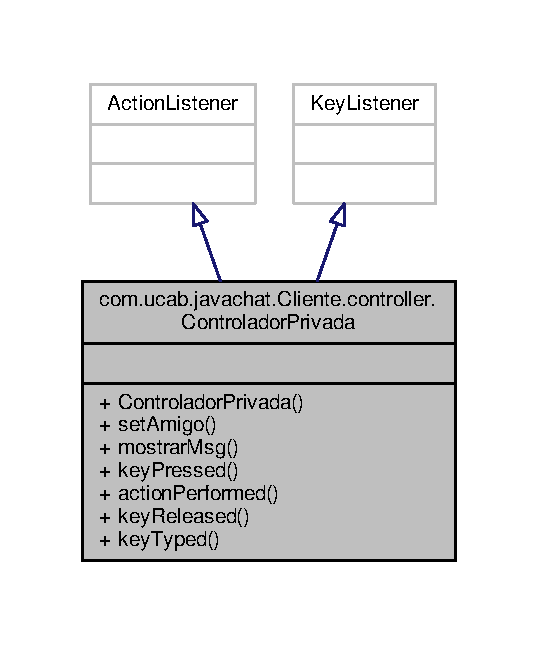
\includegraphics[width=258pt]{classcom_1_1ucab_1_1javachat_1_1_cliente_1_1controller_1_1_controlador_privada__inherit__graph}
\end{center}
\end{figure}


Diagrama de colaboración para com.\-ucab.\-javachat.\-Cliente.\-controller.\-Controlador\-Privada\-:\nopagebreak
\begin{figure}[H]
\begin{center}
\leavevmode
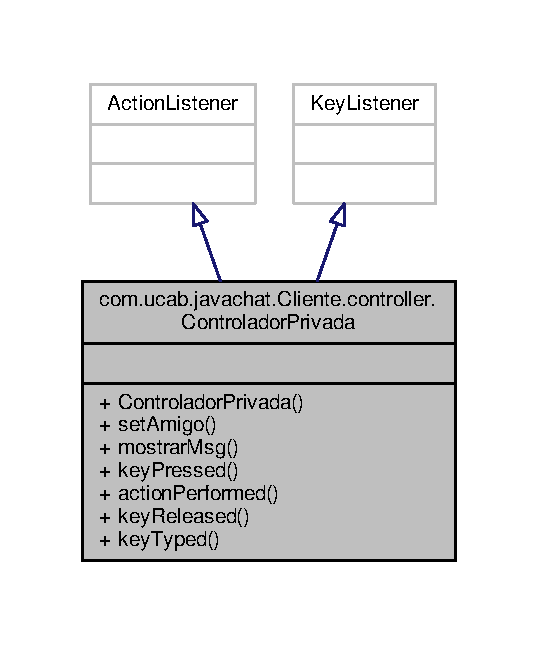
\includegraphics[width=258pt]{classcom_1_1ucab_1_1javachat_1_1_cliente_1_1controller_1_1_controlador_privada__coll__graph}
\end{center}
\end{figure}
\subsection*{Métodos públicos}
\begin{DoxyCompactItemize}
\item 
\hyperlink{classcom_1_1ucab_1_1javachat_1_1_cliente_1_1controller_1_1_controlador_privada_ad26e0344a4f4f5db7a6c61452eb3832d}{Controlador\-Privada} (\hyperlink{classcom_1_1ucab_1_1javachat_1_1_cliente_1_1view_1_1_vent_privada}{Vent\-Privada} ventana, \hyperlink{classcom_1_1ucab_1_1javachat_1_1_cliente_1_1model_1_1_cliente}{Cliente} cliente)
\item 
void \hyperlink{classcom_1_1ucab_1_1javachat_1_1_cliente_1_1controller_1_1_controlador_privada_ae7f5eb2e446616f188a05c98d0e42c17}{set\-Amigo} (Vector$<$ String $>$ amigos, String emisor)
\item 
void \hyperlink{classcom_1_1ucab_1_1javachat_1_1_cliente_1_1controller_1_1_controlador_privada_aad887b1c4f3509dcf6ae8059eaaa8d73}{mostrar\-Msg} (String msg)
\item 
void \hyperlink{classcom_1_1ucab_1_1javachat_1_1_cliente_1_1controller_1_1_controlador_privada_a779f6d7bee76a8eba068cb989d983158}{key\-Pressed} (Key\-Event e)
\item 
void \hyperlink{classcom_1_1ucab_1_1javachat_1_1_cliente_1_1controller_1_1_controlador_privada_aa3cecf9f9d16456b9a8443c92d6c3874}{action\-Performed} (Action\-Event e)
\item 
void \hyperlink{classcom_1_1ucab_1_1javachat_1_1_cliente_1_1controller_1_1_controlador_privada_abc820be85c010cffce5a09b3d8c7c9d2}{key\-Released} (Key\-Event arg0)
\item 
void \hyperlink{classcom_1_1ucab_1_1javachat_1_1_cliente_1_1controller_1_1_controlador_privada_a58b8267317cdb4bc3eb80031f82b5710}{key\-Typed} (Key\-Event arg0)
\end{DoxyCompactItemize}


\subsection{Descripción detallada}


Definición en la línea 23 del archivo Controlador\-Privada.\-java.



\subsection{Documentación del constructor y destructor}
\hypertarget{classcom_1_1ucab_1_1javachat_1_1_cliente_1_1controller_1_1_controlador_privada_ad26e0344a4f4f5db7a6c61452eb3832d}{\index{com\-::ucab\-::javachat\-::\-Cliente\-::controller\-::\-Controlador\-Privada@{com\-::ucab\-::javachat\-::\-Cliente\-::controller\-::\-Controlador\-Privada}!Controlador\-Privada@{Controlador\-Privada}}
\index{Controlador\-Privada@{Controlador\-Privada}!com::ucab::javachat::Cliente::controller::ControladorPrivada@{com\-::ucab\-::javachat\-::\-Cliente\-::controller\-::\-Controlador\-Privada}}
\subsubsection[{Controlador\-Privada}]{\setlength{\rightskip}{0pt plus 5cm}com.\-ucab.\-javachat.\-Cliente.\-controller.\-Controlador\-Privada.\-Controlador\-Privada (
\begin{DoxyParamCaption}
\item[{{\bf Vent\-Privada}}]{ventana, }
\item[{{\bf Cliente}}]{cliente}
\end{DoxyParamCaption}
)}}\label{classcom_1_1ucab_1_1javachat_1_1_cliente_1_1controller_1_1_controlador_privada_ad26e0344a4f4f5db7a6c61452eb3832d}


Definición en la línea 31 del archivo Controlador\-Privada.\-java.



\subsection{Documentación de las funciones miembro}
\hypertarget{classcom_1_1ucab_1_1javachat_1_1_cliente_1_1controller_1_1_controlador_privada_aa3cecf9f9d16456b9a8443c92d6c3874}{\index{com\-::ucab\-::javachat\-::\-Cliente\-::controller\-::\-Controlador\-Privada@{com\-::ucab\-::javachat\-::\-Cliente\-::controller\-::\-Controlador\-Privada}!action\-Performed@{action\-Performed}}
\index{action\-Performed@{action\-Performed}!com::ucab::javachat::Cliente::controller::ControladorPrivada@{com\-::ucab\-::javachat\-::\-Cliente\-::controller\-::\-Controlador\-Privada}}
\subsubsection[{action\-Performed}]{\setlength{\rightskip}{0pt plus 5cm}void com.\-ucab.\-javachat.\-Cliente.\-controller.\-Controlador\-Privada.\-action\-Performed (
\begin{DoxyParamCaption}
\item[{Action\-Event}]{e}
\end{DoxyParamCaption}
)}}\label{classcom_1_1ucab_1_1javachat_1_1_cliente_1_1controller_1_1_controlador_privada_aa3cecf9f9d16456b9a8443c92d6c3874}


Definición en la línea 125 del archivo Controlador\-Privada.\-java.

\hypertarget{classcom_1_1ucab_1_1javachat_1_1_cliente_1_1controller_1_1_controlador_privada_a779f6d7bee76a8eba068cb989d983158}{\index{com\-::ucab\-::javachat\-::\-Cliente\-::controller\-::\-Controlador\-Privada@{com\-::ucab\-::javachat\-::\-Cliente\-::controller\-::\-Controlador\-Privada}!key\-Pressed@{key\-Pressed}}
\index{key\-Pressed@{key\-Pressed}!com::ucab::javachat::Cliente::controller::ControladorPrivada@{com\-::ucab\-::javachat\-::\-Cliente\-::controller\-::\-Controlador\-Privada}}
\subsubsection[{key\-Pressed}]{\setlength{\rightskip}{0pt plus 5cm}void com.\-ucab.\-javachat.\-Cliente.\-controller.\-Controlador\-Privada.\-key\-Pressed (
\begin{DoxyParamCaption}
\item[{Key\-Event}]{e}
\end{DoxyParamCaption}
)}}\label{classcom_1_1ucab_1_1javachat_1_1_cliente_1_1controller_1_1_controlador_privada_a779f6d7bee76a8eba068cb989d983158}


Definición en la línea 100 del archivo Controlador\-Privada.\-java.

\hypertarget{classcom_1_1ucab_1_1javachat_1_1_cliente_1_1controller_1_1_controlador_privada_abc820be85c010cffce5a09b3d8c7c9d2}{\index{com\-::ucab\-::javachat\-::\-Cliente\-::controller\-::\-Controlador\-Privada@{com\-::ucab\-::javachat\-::\-Cliente\-::controller\-::\-Controlador\-Privada}!key\-Released@{key\-Released}}
\index{key\-Released@{key\-Released}!com::ucab::javachat::Cliente::controller::ControladorPrivada@{com\-::ucab\-::javachat\-::\-Cliente\-::controller\-::\-Controlador\-Privada}}
\subsubsection[{key\-Released}]{\setlength{\rightskip}{0pt plus 5cm}void com.\-ucab.\-javachat.\-Cliente.\-controller.\-Controlador\-Privada.\-key\-Released (
\begin{DoxyParamCaption}
\item[{Key\-Event}]{arg0}
\end{DoxyParamCaption}
)}}\label{classcom_1_1ucab_1_1javachat_1_1_cliente_1_1controller_1_1_controlador_privada_abc820be85c010cffce5a09b3d8c7c9d2}


Definición en la línea 167 del archivo Controlador\-Privada.\-java.

\hypertarget{classcom_1_1ucab_1_1javachat_1_1_cliente_1_1controller_1_1_controlador_privada_a58b8267317cdb4bc3eb80031f82b5710}{\index{com\-::ucab\-::javachat\-::\-Cliente\-::controller\-::\-Controlador\-Privada@{com\-::ucab\-::javachat\-::\-Cliente\-::controller\-::\-Controlador\-Privada}!key\-Typed@{key\-Typed}}
\index{key\-Typed@{key\-Typed}!com::ucab::javachat::Cliente::controller::ControladorPrivada@{com\-::ucab\-::javachat\-::\-Cliente\-::controller\-::\-Controlador\-Privada}}
\subsubsection[{key\-Typed}]{\setlength{\rightskip}{0pt plus 5cm}void com.\-ucab.\-javachat.\-Cliente.\-controller.\-Controlador\-Privada.\-key\-Typed (
\begin{DoxyParamCaption}
\item[{Key\-Event}]{arg0}
\end{DoxyParamCaption}
)}}\label{classcom_1_1ucab_1_1javachat_1_1_cliente_1_1controller_1_1_controlador_privada_a58b8267317cdb4bc3eb80031f82b5710}


Definición en la línea 173 del archivo Controlador\-Privada.\-java.

\hypertarget{classcom_1_1ucab_1_1javachat_1_1_cliente_1_1controller_1_1_controlador_privada_aad887b1c4f3509dcf6ae8059eaaa8d73}{\index{com\-::ucab\-::javachat\-::\-Cliente\-::controller\-::\-Controlador\-Privada@{com\-::ucab\-::javachat\-::\-Cliente\-::controller\-::\-Controlador\-Privada}!mostrar\-Msg@{mostrar\-Msg}}
\index{mostrar\-Msg@{mostrar\-Msg}!com::ucab::javachat::Cliente::controller::ControladorPrivada@{com\-::ucab\-::javachat\-::\-Cliente\-::controller\-::\-Controlador\-Privada}}
\subsubsection[{mostrar\-Msg}]{\setlength{\rightskip}{0pt plus 5cm}void com.\-ucab.\-javachat.\-Cliente.\-controller.\-Controlador\-Privada.\-mostrar\-Msg (
\begin{DoxyParamCaption}
\item[{String}]{msg}
\end{DoxyParamCaption}
)}}\label{classcom_1_1ucab_1_1javachat_1_1_cliente_1_1controller_1_1_controlador_privada_aad887b1c4f3509dcf6ae8059eaaa8d73}


Definición en la línea 82 del archivo Controlador\-Privada.\-java.

\hypertarget{classcom_1_1ucab_1_1javachat_1_1_cliente_1_1controller_1_1_controlador_privada_ae7f5eb2e446616f188a05c98d0e42c17}{\index{com\-::ucab\-::javachat\-::\-Cliente\-::controller\-::\-Controlador\-Privada@{com\-::ucab\-::javachat\-::\-Cliente\-::controller\-::\-Controlador\-Privada}!set\-Amigo@{set\-Amigo}}
\index{set\-Amigo@{set\-Amigo}!com::ucab::javachat::Cliente::controller::ControladorPrivada@{com\-::ucab\-::javachat\-::\-Cliente\-::controller\-::\-Controlador\-Privada}}
\subsubsection[{set\-Amigo}]{\setlength{\rightskip}{0pt plus 5cm}void com.\-ucab.\-javachat.\-Cliente.\-controller.\-Controlador\-Privada.\-set\-Amigo (
\begin{DoxyParamCaption}
\item[{Vector$<$ String $>$}]{amigos, }
\item[{String}]{emisor}
\end{DoxyParamCaption}
)}}\label{classcom_1_1ucab_1_1javachat_1_1_cliente_1_1controller_1_1_controlador_privada_ae7f5eb2e446616f188a05c98d0e42c17}


Definición en la línea 54 del archivo Controlador\-Privada.\-java.



La documentación para esta clase fue generada a partir del siguiente fichero\-:\begin{DoxyCompactItemize}
\item 
Escritorio/\-Chat\-Morse/src/com/ucab/javachat/\-Cliente/controller/\hyperlink{_controlador_privada_8java}{Controlador\-Privada.\-java}\end{DoxyCompactItemize}

\hypertarget{classcom_1_1ucab_1_1javachat_1_1_cliente_1_1controller_1_1_controlador_recuperar_contrase_xC3_xB1a}{\section{Referencia de la Clase com.\-ucab.\-javachat.\-Cliente.\-controller.\-Controlador\-Recuperar\-Contraseña}
\label{classcom_1_1ucab_1_1javachat_1_1_cliente_1_1controller_1_1_controlador_recuperar_contrase_xC3_xB1a}\index{com.\-ucab.\-javachat.\-Cliente.\-controller.\-Controlador\-Recuperar\-Contraseña@{com.\-ucab.\-javachat.\-Cliente.\-controller.\-Controlador\-Recuperar\-Contraseña}}
}


Diagrama de herencias de com.\-ucab.\-javachat.\-Cliente.\-controller.\-Controlador\-Recuperar\-Contraseña
\nopagebreak
\begin{figure}[H]
\begin{center}
\leavevmode
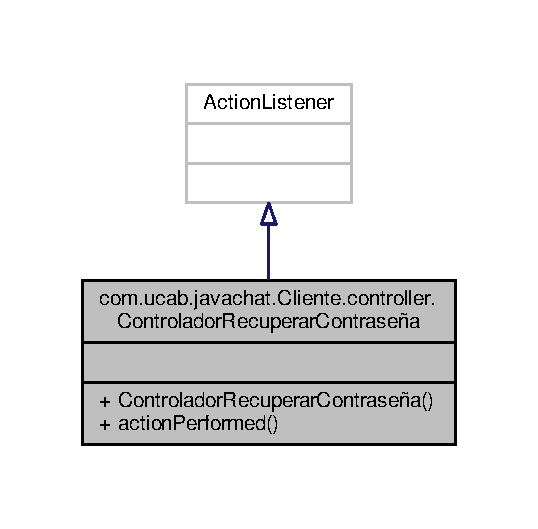
\includegraphics[width=258pt]{d0/da0/classcom_1_1ucab_1_1javachat_1_1_cliente_1_1controller_1_1_controlador_recuperar_contrase_xC3_xB1a__inherit__graph}
\end{center}
\end{figure}


Diagrama de colaboración para com.\-ucab.\-javachat.\-Cliente.\-controller.\-Controlador\-Recuperar\-Contraseña\-:
\nopagebreak
\begin{figure}[H]
\begin{center}
\leavevmode
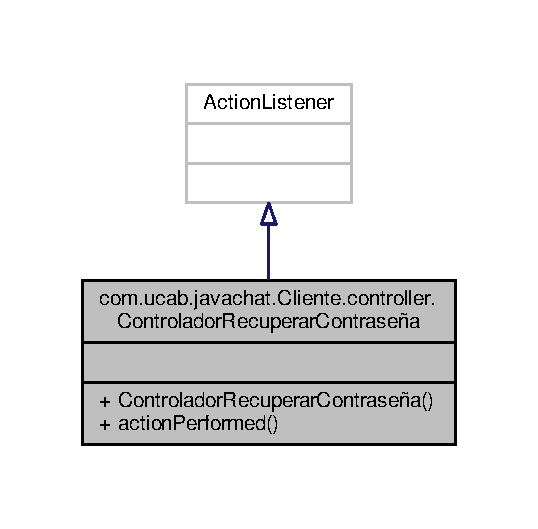
\includegraphics[width=258pt]{d1/def/classcom_1_1ucab_1_1javachat_1_1_cliente_1_1controller_1_1_controlador_recuperar_contrase_xC3_xB1a__coll__graph}
\end{center}
\end{figure}
\subsection*{Métodos públicos}
\begin{DoxyCompactItemize}
\item 
\hypertarget{classcom_1_1ucab_1_1javachat_1_1_cliente_1_1controller_1_1_controlador_recuperar_contrase_xC3_xB1a_a9bf650dbd9bd8af042b92a43baa80111}{{\bfseries Controlador\-Recuperar\-Contraseña} (\hyperlink{classcom_1_1ucab_1_1javachat_1_1_cliente_1_1view_1_1_vent_recuperar_contrase_xC3_xB1a}{Vent\-Recuperar\-Contraseña} vista)}\label{classcom_1_1ucab_1_1javachat_1_1_cliente_1_1controller_1_1_controlador_recuperar_contrase_xC3_xB1a_a9bf650dbd9bd8af042b92a43baa80111}

\item 
void \hyperlink{classcom_1_1ucab_1_1javachat_1_1_cliente_1_1controller_1_1_controlador_recuperar_contrase_xC3_xB1a_a3e2d23c7eea7fa3a47b41cb6638d2335}{action\-Performed} (Action\-Event e)
\end{DoxyCompactItemize}


\subsection{Descripción detallada}
Clase encargada de controlar la ventana de Recuperar contraseña \begin{DoxyAuthor}{Autor}
Grupo 3 
\end{DoxyAuthor}


Definición en la línea 23 del archivo Controlador\-Recuperar\-Contraseña.\-java.



\subsection{Documentación de las funciones miembro}
\hypertarget{classcom_1_1ucab_1_1javachat_1_1_cliente_1_1controller_1_1_controlador_recuperar_contrase_xC3_xB1a_a3e2d23c7eea7fa3a47b41cb6638d2335}{\index{com\-::ucab\-::javachat\-::\-Cliente\-::controller\-::\-Controlador\-Recuperar\-Contraseña@{com\-::ucab\-::javachat\-::\-Cliente\-::controller\-::\-Controlador\-Recuperar\-Contraseña}!action\-Performed@{action\-Performed}}
\index{action\-Performed@{action\-Performed}!com::ucab::javachat::Cliente::controller::ControladorRecuperarContraseña@{com\-::ucab\-::javachat\-::\-Cliente\-::controller\-::\-Controlador\-Recuperar\-Contraseña}}
\subsubsection[{action\-Performed}]{\setlength{\rightskip}{0pt plus 5cm}void com.\-ucab.\-javachat.\-Cliente.\-controller.\-Controlador\-Recuperar\-Contraseña.\-action\-Performed (
\begin{DoxyParamCaption}
\item[{Action\-Event}]{e}
\end{DoxyParamCaption}
)}}\label{classcom_1_1ucab_1_1javachat_1_1_cliente_1_1controller_1_1_controlador_recuperar_contrase_xC3_xB1a_a3e2d23c7eea7fa3a47b41cb6638d2335}
metodo encargado de la accion de cada boton y/o campo de texto que se encuentra en la ventana 

Definición en la línea 41 del archivo Controlador\-Recuperar\-Contraseña.\-java.



Gráfico de llamadas para esta función\-:
\nopagebreak
\begin{figure}[H]
\begin{center}
\leavevmode
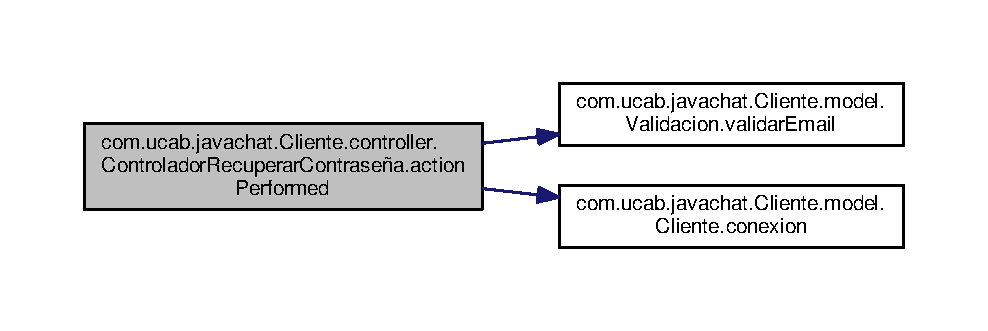
\includegraphics[width=350pt]{dd/dd6/classcom_1_1ucab_1_1javachat_1_1_cliente_1_1controller_1_1_controlador_recuperar_contrase_xC3_xB1a_a3e2d23c7eea7fa3a47b41cb6638d2335_cgraph}
\end{center}
\end{figure}




La documentación para esta clase fue generada a partir del siguiente fichero\-:\begin{DoxyCompactItemize}
\item 
Chat-\/\-Codigo-\/\-Morse/\-Chat\-Morse/src/com/ucab/javachat/\-Cliente/controller/Controlador\-Recuperar\-Contraseña.\-java\end{DoxyCompactItemize}

\hypertarget{classcom_1_1ucab_1_1javachat_1_1_cliente_1_1controller_1_1_controlador_registrar_usuario}{\section{Referencia de la Clase com.\-ucab.\-javachat.\-Cliente.\-controller.\-Controlador\-Registrar\-Usuario}
\label{classcom_1_1ucab_1_1javachat_1_1_cliente_1_1controller_1_1_controlador_registrar_usuario}\index{com.\-ucab.\-javachat.\-Cliente.\-controller.\-Controlador\-Registrar\-Usuario@{com.\-ucab.\-javachat.\-Cliente.\-controller.\-Controlador\-Registrar\-Usuario}}
}


Diagrama de herencias de com.\-ucab.\-javachat.\-Cliente.\-controller.\-Controlador\-Registrar\-Usuario\nopagebreak
\begin{figure}[H]
\begin{center}
\leavevmode
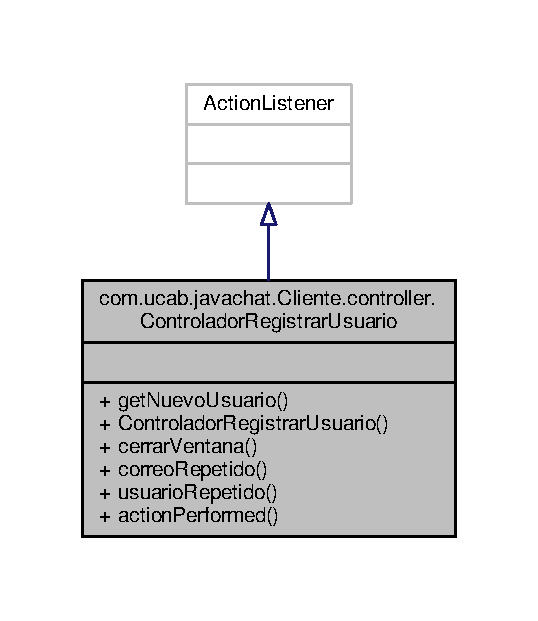
\includegraphics[width=258pt]{classcom_1_1ucab_1_1javachat_1_1_cliente_1_1controller_1_1_controlador_registrar_usuario__inherit__graph}
\end{center}
\end{figure}


Diagrama de colaboración para com.\-ucab.\-javachat.\-Cliente.\-controller.\-Controlador\-Registrar\-Usuario\-:\nopagebreak
\begin{figure}[H]
\begin{center}
\leavevmode
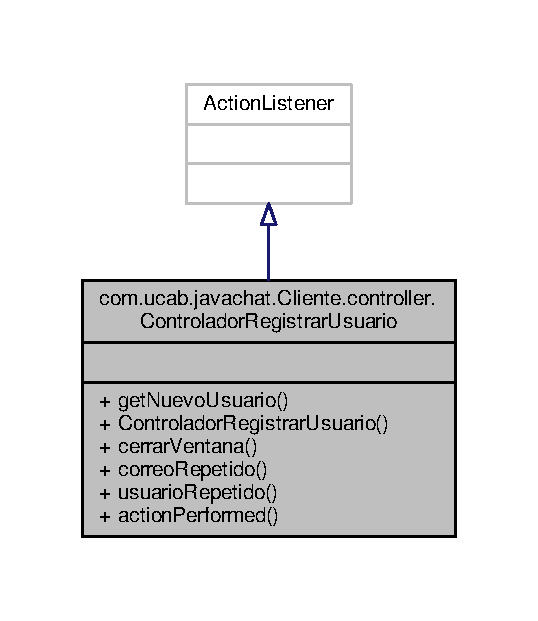
\includegraphics[width=258pt]{classcom_1_1ucab_1_1javachat_1_1_cliente_1_1controller_1_1_controlador_registrar_usuario__coll__graph}
\end{center}
\end{figure}
\subsection*{Métodos públicos}
\begin{DoxyCompactItemize}
\item 
\hyperlink{classcom_1_1ucab_1_1javachat_1_1_cliente_1_1model_1_1_usuario}{Usuario} \hyperlink{classcom_1_1ucab_1_1javachat_1_1_cliente_1_1controller_1_1_controlador_registrar_usuario_ae74c423df59d850fce66dc1ba049c563}{get\-Nuevo\-Usuario} ()
\item 
\hyperlink{classcom_1_1ucab_1_1javachat_1_1_cliente_1_1controller_1_1_controlador_registrar_usuario_ac501d29a542346226190021b56b11288}{Controlador\-Registrar\-Usuario} (\hyperlink{classcom_1_1ucab_1_1javachat_1_1_cliente_1_1view_1_1_vent_registro}{Vent\-Registro} vista)
\item 
void \hyperlink{classcom_1_1ucab_1_1javachat_1_1_cliente_1_1controller_1_1_controlador_registrar_usuario_a02bbff561df82eb06a129f6f12e33a35}{cerrar\-Ventana} ()
\item 
void \hyperlink{classcom_1_1ucab_1_1javachat_1_1_cliente_1_1controller_1_1_controlador_registrar_usuario_a803aeb4dc6e260ee0eb1be7e5603e088}{correo\-Repetido} ()
\item 
void \hyperlink{classcom_1_1ucab_1_1javachat_1_1_cliente_1_1controller_1_1_controlador_registrar_usuario_a340270aa28a899021ee92469aad2e270}{usuario\-Repetido} ()
\item 
void \hyperlink{classcom_1_1ucab_1_1javachat_1_1_cliente_1_1controller_1_1_controlador_registrar_usuario_a45806ea9b7bbbc99883ecb5a521ecf3b}{action\-Performed} (Action\-Event e)
\end{DoxyCompactItemize}


\subsection{Descripción detallada}
Esta clase es el controlador de la vista del registro de usuario. Al usuario se le indica con que caracteristica especifica debe contar cada campo de registro. Luego se obtiene la informacion indicada en los campos mostrados en las vista y se aplican los metodos necesarios para la comprobacion de la informacion. Si todos los campos estan correctamente rellenados, se procede a enviar la información al servidor para guardarla.

\begin{DoxyAuthor}{Autores}
Grupo 3 -\/ A. Rodriguez, I. Teixeira, L. Valladares, D. Suarez 
\end{DoxyAuthor}
\begin{DoxyVersion}{Versión}
2.\-0 
\end{DoxyVersion}


Definición en la línea 30 del archivo Controlador\-Registrar\-Usuario.\-java.



\subsection{Documentación del constructor y destructor}
\hypertarget{classcom_1_1ucab_1_1javachat_1_1_cliente_1_1controller_1_1_controlador_registrar_usuario_ac501d29a542346226190021b56b11288}{\index{com\-::ucab\-::javachat\-::\-Cliente\-::controller\-::\-Controlador\-Registrar\-Usuario@{com\-::ucab\-::javachat\-::\-Cliente\-::controller\-::\-Controlador\-Registrar\-Usuario}!Controlador\-Registrar\-Usuario@{Controlador\-Registrar\-Usuario}}
\index{Controlador\-Registrar\-Usuario@{Controlador\-Registrar\-Usuario}!com::ucab::javachat::Cliente::controller::ControladorRegistrarUsuario@{com\-::ucab\-::javachat\-::\-Cliente\-::controller\-::\-Controlador\-Registrar\-Usuario}}
\subsubsection[{Controlador\-Registrar\-Usuario}]{\setlength{\rightskip}{0pt plus 5cm}com.\-ucab.\-javachat.\-Cliente.\-controller.\-Controlador\-Registrar\-Usuario.\-Controlador\-Registrar\-Usuario (
\begin{DoxyParamCaption}
\item[{{\bf Vent\-Registro}}]{vista}
\end{DoxyParamCaption}
)}}\label{classcom_1_1ucab_1_1javachat_1_1_cliente_1_1controller_1_1_controlador_registrar_usuario_ac501d29a542346226190021b56b11288}
Constructor del controlador. Aqui se añaden los Listener a los botones de la vista. 
\begin{DoxyParams}{Parámetros}
{\em vista} & -\/ Instancia de la ventana para registrar al usuario. \\
\hline
{\em cliente} & -\/ Instancia del modelo en el que se envian los datos del usuario al servidor. \\
\hline
\end{DoxyParams}


Definición en la línea 45 del archivo Controlador\-Registrar\-Usuario.\-java.



\subsection{Documentación de las funciones miembro}
\hypertarget{classcom_1_1ucab_1_1javachat_1_1_cliente_1_1controller_1_1_controlador_registrar_usuario_a45806ea9b7bbbc99883ecb5a521ecf3b}{\index{com\-::ucab\-::javachat\-::\-Cliente\-::controller\-::\-Controlador\-Registrar\-Usuario@{com\-::ucab\-::javachat\-::\-Cliente\-::controller\-::\-Controlador\-Registrar\-Usuario}!action\-Performed@{action\-Performed}}
\index{action\-Performed@{action\-Performed}!com::ucab::javachat::Cliente::controller::ControladorRegistrarUsuario@{com\-::ucab\-::javachat\-::\-Cliente\-::controller\-::\-Controlador\-Registrar\-Usuario}}
\subsubsection[{action\-Performed}]{\setlength{\rightskip}{0pt plus 5cm}void com.\-ucab.\-javachat.\-Cliente.\-controller.\-Controlador\-Registrar\-Usuario.\-action\-Performed (
\begin{DoxyParamCaption}
\item[{Action\-Event}]{e}
\end{DoxyParamCaption}
)}}\label{classcom_1_1ucab_1_1javachat_1_1_cliente_1_1controller_1_1_controlador_registrar_usuario_a45806ea9b7bbbc99883ecb5a521ecf3b}
Controlador de eventos para los botones de la vista. 

Definición en la línea 72 del archivo Controlador\-Registrar\-Usuario.\-java.



Gráfico de llamadas para esta función\-:\nopagebreak
\begin{figure}[H]
\begin{center}
\leavevmode
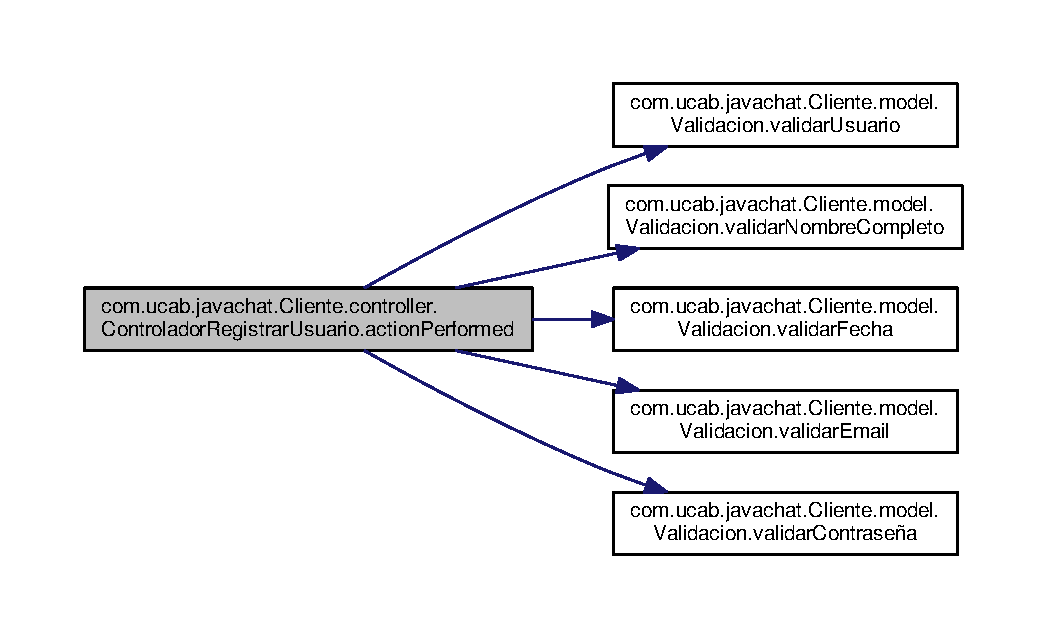
\includegraphics[width=350pt]{classcom_1_1ucab_1_1javachat_1_1_cliente_1_1controller_1_1_controlador_registrar_usuario_a45806ea9b7bbbc99883ecb5a521ecf3b_cgraph}
\end{center}
\end{figure}


\hypertarget{classcom_1_1ucab_1_1javachat_1_1_cliente_1_1controller_1_1_controlador_registrar_usuario_a02bbff561df82eb06a129f6f12e33a35}{\index{com\-::ucab\-::javachat\-::\-Cliente\-::controller\-::\-Controlador\-Registrar\-Usuario@{com\-::ucab\-::javachat\-::\-Cliente\-::controller\-::\-Controlador\-Registrar\-Usuario}!cerrar\-Ventana@{cerrar\-Ventana}}
\index{cerrar\-Ventana@{cerrar\-Ventana}!com::ucab::javachat::Cliente::controller::ControladorRegistrarUsuario@{com\-::ucab\-::javachat\-::\-Cliente\-::controller\-::\-Controlador\-Registrar\-Usuario}}
\subsubsection[{cerrar\-Ventana}]{\setlength{\rightskip}{0pt plus 5cm}void com.\-ucab.\-javachat.\-Cliente.\-controller.\-Controlador\-Registrar\-Usuario.\-cerrar\-Ventana (
\begin{DoxyParamCaption}
{}
\end{DoxyParamCaption}
)}}\label{classcom_1_1ucab_1_1javachat_1_1_cliente_1_1controller_1_1_controlador_registrar_usuario_a02bbff561df82eb06a129f6f12e33a35}


Definición en la línea 55 del archivo Controlador\-Registrar\-Usuario.\-java.

\hypertarget{classcom_1_1ucab_1_1javachat_1_1_cliente_1_1controller_1_1_controlador_registrar_usuario_a803aeb4dc6e260ee0eb1be7e5603e088}{\index{com\-::ucab\-::javachat\-::\-Cliente\-::controller\-::\-Controlador\-Registrar\-Usuario@{com\-::ucab\-::javachat\-::\-Cliente\-::controller\-::\-Controlador\-Registrar\-Usuario}!correo\-Repetido@{correo\-Repetido}}
\index{correo\-Repetido@{correo\-Repetido}!com::ucab::javachat::Cliente::controller::ControladorRegistrarUsuario@{com\-::ucab\-::javachat\-::\-Cliente\-::controller\-::\-Controlador\-Registrar\-Usuario}}
\subsubsection[{correo\-Repetido}]{\setlength{\rightskip}{0pt plus 5cm}void com.\-ucab.\-javachat.\-Cliente.\-controller.\-Controlador\-Registrar\-Usuario.\-correo\-Repetido (
\begin{DoxyParamCaption}
{}
\end{DoxyParamCaption}
)}}\label{classcom_1_1ucab_1_1javachat_1_1_cliente_1_1controller_1_1_controlador_registrar_usuario_a803aeb4dc6e260ee0eb1be7e5603e088}


Definición en la línea 59 del archivo Controlador\-Registrar\-Usuario.\-java.

\hypertarget{classcom_1_1ucab_1_1javachat_1_1_cliente_1_1controller_1_1_controlador_registrar_usuario_ae74c423df59d850fce66dc1ba049c563}{\index{com\-::ucab\-::javachat\-::\-Cliente\-::controller\-::\-Controlador\-Registrar\-Usuario@{com\-::ucab\-::javachat\-::\-Cliente\-::controller\-::\-Controlador\-Registrar\-Usuario}!get\-Nuevo\-Usuario@{get\-Nuevo\-Usuario}}
\index{get\-Nuevo\-Usuario@{get\-Nuevo\-Usuario}!com::ucab::javachat::Cliente::controller::ControladorRegistrarUsuario@{com\-::ucab\-::javachat\-::\-Cliente\-::controller\-::\-Controlador\-Registrar\-Usuario}}
\subsubsection[{get\-Nuevo\-Usuario}]{\setlength{\rightskip}{0pt plus 5cm}{\bf Usuario} com.\-ucab.\-javachat.\-Cliente.\-controller.\-Controlador\-Registrar\-Usuario.\-get\-Nuevo\-Usuario (
\begin{DoxyParamCaption}
{}
\end{DoxyParamCaption}
)}}\label{classcom_1_1ucab_1_1javachat_1_1_cliente_1_1controller_1_1_controlador_registrar_usuario_ae74c423df59d850fce66dc1ba049c563}


Definición en la línea 36 del archivo Controlador\-Registrar\-Usuario.\-java.

\hypertarget{classcom_1_1ucab_1_1javachat_1_1_cliente_1_1controller_1_1_controlador_registrar_usuario_a340270aa28a899021ee92469aad2e270}{\index{com\-::ucab\-::javachat\-::\-Cliente\-::controller\-::\-Controlador\-Registrar\-Usuario@{com\-::ucab\-::javachat\-::\-Cliente\-::controller\-::\-Controlador\-Registrar\-Usuario}!usuario\-Repetido@{usuario\-Repetido}}
\index{usuario\-Repetido@{usuario\-Repetido}!com::ucab::javachat::Cliente::controller::ControladorRegistrarUsuario@{com\-::ucab\-::javachat\-::\-Cliente\-::controller\-::\-Controlador\-Registrar\-Usuario}}
\subsubsection[{usuario\-Repetido}]{\setlength{\rightskip}{0pt plus 5cm}void com.\-ucab.\-javachat.\-Cliente.\-controller.\-Controlador\-Registrar\-Usuario.\-usuario\-Repetido (
\begin{DoxyParamCaption}
{}
\end{DoxyParamCaption}
)}}\label{classcom_1_1ucab_1_1javachat_1_1_cliente_1_1controller_1_1_controlador_registrar_usuario_a340270aa28a899021ee92469aad2e270}


Definición en la línea 64 del archivo Controlador\-Registrar\-Usuario.\-java.



La documentación para esta clase fue generada a partir del siguiente fichero\-:\begin{DoxyCompactItemize}
\item 
Escritorio/\-Chat\-Morse/src/com/ucab/javachat/\-Cliente/controller/\hyperlink{_controlador_registrar_usuario_8java}{Controlador\-Registrar\-Usuario.\-java}\end{DoxyCompactItemize}

\hypertarget{classcom_1_1ucab_1_1javachat_1_1_cliente_1_1model_1_1_criptologia}{\section{Referencia de la Clase com.\-ucab.\-javachat.\-Cliente.\-model.\-Criptologia}
\label{classcom_1_1ucab_1_1javachat_1_1_cliente_1_1model_1_1_criptologia}\index{com.\-ucab.\-javachat.\-Cliente.\-model.\-Criptologia@{com.\-ucab.\-javachat.\-Cliente.\-model.\-Criptologia}}
}


Diagrama de colaboración para com.\-ucab.\-javachat.\-Cliente.\-model.\-Criptologia\-:\nopagebreak
\begin{figure}[H]
\begin{center}
\leavevmode
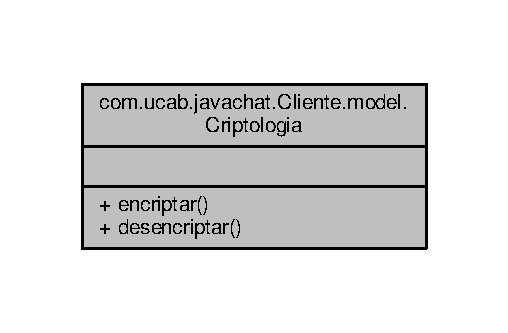
\includegraphics[width=244pt]{classcom_1_1ucab_1_1javachat_1_1_cliente_1_1model_1_1_criptologia__coll__graph}
\end{center}
\end{figure}
\subsection*{Métodos públicos estáticos}
\begin{DoxyCompactItemize}
\item 
static String \hyperlink{classcom_1_1ucab_1_1javachat_1_1_cliente_1_1model_1_1_criptologia_ae1dd0633e8f03d5a9ca3738ea7073275}{encriptar} (String texto)
\item 
static String \hyperlink{classcom_1_1ucab_1_1javachat_1_1_cliente_1_1model_1_1_criptologia_a00407379cf4e57988ad22d24d3e58505}{desencriptar} (String texto\-Encriptado)  throws Exception 
\end{DoxyCompactItemize}


\subsection{Descripción detallada}
Esta clase tiene los metodos para encriptar y desencriptar la informacion importante del usuario.

Los metodos los consegui de\-: //http\-://www.qualityinfosolutions.\-com/metodos-\/para-\/encriptar-\/y-\/desencriptar-\/en-\/java/

\begin{DoxyAuthor}{Autor}
qualitifuinfosolutions. 
\end{DoxyAuthor}


Definición en la línea 24 del archivo Criptologia.\-java.



\subsection{Documentación de las funciones miembro}
\hypertarget{classcom_1_1ucab_1_1javachat_1_1_cliente_1_1model_1_1_criptologia_a00407379cf4e57988ad22d24d3e58505}{\index{com\-::ucab\-::javachat\-::\-Cliente\-::model\-::\-Criptologia@{com\-::ucab\-::javachat\-::\-Cliente\-::model\-::\-Criptologia}!desencriptar@{desencriptar}}
\index{desencriptar@{desencriptar}!com::ucab::javachat::Cliente::model::Criptologia@{com\-::ucab\-::javachat\-::\-Cliente\-::model\-::\-Criptologia}}
\subsubsection[{desencriptar}]{\setlength{\rightskip}{0pt plus 5cm}static String com.\-ucab.\-javachat.\-Cliente.\-model.\-Criptologia.\-desencriptar (
\begin{DoxyParamCaption}
\item[{String}]{texto\-Encriptado}
\end{DoxyParamCaption}
) throws Exception\hspace{0.3cm}{\ttfamily [static]}}}\label{classcom_1_1ucab_1_1javachat_1_1_cliente_1_1model_1_1_criptologia_a00407379cf4e57988ad22d24d3e58505}


Definición en la línea 52 del archivo Criptologia.\-java.

\hypertarget{classcom_1_1ucab_1_1javachat_1_1_cliente_1_1model_1_1_criptologia_ae1dd0633e8f03d5a9ca3738ea7073275}{\index{com\-::ucab\-::javachat\-::\-Cliente\-::model\-::\-Criptologia@{com\-::ucab\-::javachat\-::\-Cliente\-::model\-::\-Criptologia}!encriptar@{encriptar}}
\index{encriptar@{encriptar}!com::ucab::javachat::Cliente::model::Criptologia@{com\-::ucab\-::javachat\-::\-Cliente\-::model\-::\-Criptologia}}
\subsubsection[{encriptar}]{\setlength{\rightskip}{0pt plus 5cm}static String com.\-ucab.\-javachat.\-Cliente.\-model.\-Criptologia.\-encriptar (
\begin{DoxyParamCaption}
\item[{String}]{texto}
\end{DoxyParamCaption}
)\hspace{0.3cm}{\ttfamily [static]}}}\label{classcom_1_1ucab_1_1javachat_1_1_cliente_1_1model_1_1_criptologia_ae1dd0633e8f03d5a9ca3738ea7073275}


Definición en la línea 26 del archivo Criptologia.\-java.



Gráfico de llamadas a esta función\-:\nopagebreak
\begin{figure}[H]
\begin{center}
\leavevmode
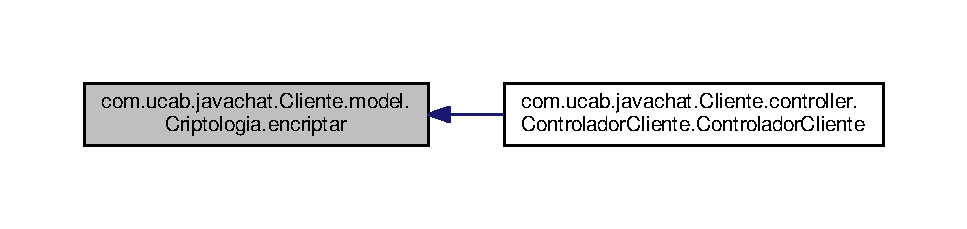
\includegraphics[width=350pt]{classcom_1_1ucab_1_1javachat_1_1_cliente_1_1model_1_1_criptologia_ae1dd0633e8f03d5a9ca3738ea7073275_icgraph}
\end{center}
\end{figure}




La documentación para esta clase fue generada a partir del siguiente fichero\-:\begin{DoxyCompactItemize}
\item 
Escritorio/\-Chat\-Morse/src/com/ucab/javachat/\-Cliente/model/\hyperlink{_cliente_2model_2_criptologia_8java}{Criptologia.\-java}\end{DoxyCompactItemize}

\hypertarget{classcom_1_1ucab_1_1javachat_1_1_servidor_1_1model_1_1_criptologia}{\section{Referencia de la Clase com.\-ucab.\-javachat.\-Servidor.\-model.\-Criptologia}
\label{classcom_1_1ucab_1_1javachat_1_1_servidor_1_1model_1_1_criptologia}\index{com.\-ucab.\-javachat.\-Servidor.\-model.\-Criptologia@{com.\-ucab.\-javachat.\-Servidor.\-model.\-Criptologia}}
}


Diagrama de colaboración para com.\-ucab.\-javachat.\-Servidor.\-model.\-Criptologia\-:\nopagebreak
\begin{figure}[H]
\begin{center}
\leavevmode
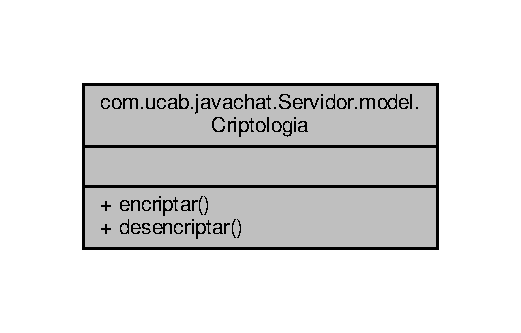
\includegraphics[width=250pt]{classcom_1_1ucab_1_1javachat_1_1_servidor_1_1model_1_1_criptologia__coll__graph}
\end{center}
\end{figure}
\subsection*{Métodos públicos estáticos}
\begin{DoxyCompactItemize}
\item 
static String \hyperlink{classcom_1_1ucab_1_1javachat_1_1_servidor_1_1model_1_1_criptologia_a0a816425dbef403c92d0f858e6a910cd}{encriptar} (String texto)
\item 
static String \hyperlink{classcom_1_1ucab_1_1javachat_1_1_servidor_1_1model_1_1_criptologia_ae580b0995ce546a2e8b37c819651d240}{desencriptar} (String texto\-Encriptado)
\end{DoxyCompactItemize}


\subsection{Descripción detallada}
Esta clase tiene los metodos para encriptar y desencriptar la informacion importante del usuario.

Los metodos los consegui de\-: //http\-://www.qualityinfosolutions.\-com/metodos-\/para-\/encriptar-\/y-\/desencriptar-\/en-\/java/

\begin{DoxyAuthor}{Autor}
qualitifuinfosolutions. 
\end{DoxyAuthor}


Definición en la línea 22 del archivo Criptologia.\-java.



\subsection{Documentación de las funciones miembro}
\hypertarget{classcom_1_1ucab_1_1javachat_1_1_servidor_1_1model_1_1_criptologia_ae580b0995ce546a2e8b37c819651d240}{\index{com\-::ucab\-::javachat\-::\-Servidor\-::model\-::\-Criptologia@{com\-::ucab\-::javachat\-::\-Servidor\-::model\-::\-Criptologia}!desencriptar@{desencriptar}}
\index{desencriptar@{desencriptar}!com::ucab::javachat::Servidor::model::Criptologia@{com\-::ucab\-::javachat\-::\-Servidor\-::model\-::\-Criptologia}}
\subsubsection[{desencriptar}]{\setlength{\rightskip}{0pt plus 5cm}static String com.\-ucab.\-javachat.\-Servidor.\-model.\-Criptologia.\-desencriptar (
\begin{DoxyParamCaption}
\item[{String}]{texto\-Encriptado}
\end{DoxyParamCaption}
)\hspace{0.3cm}{\ttfamily [static]}}}\label{classcom_1_1ucab_1_1javachat_1_1_servidor_1_1model_1_1_criptologia_ae580b0995ce546a2e8b37c819651d240}


Definición en la línea 49 del archivo Criptologia.\-java.



Gráfico de llamadas a esta función\-:\nopagebreak
\begin{figure}[H]
\begin{center}
\leavevmode
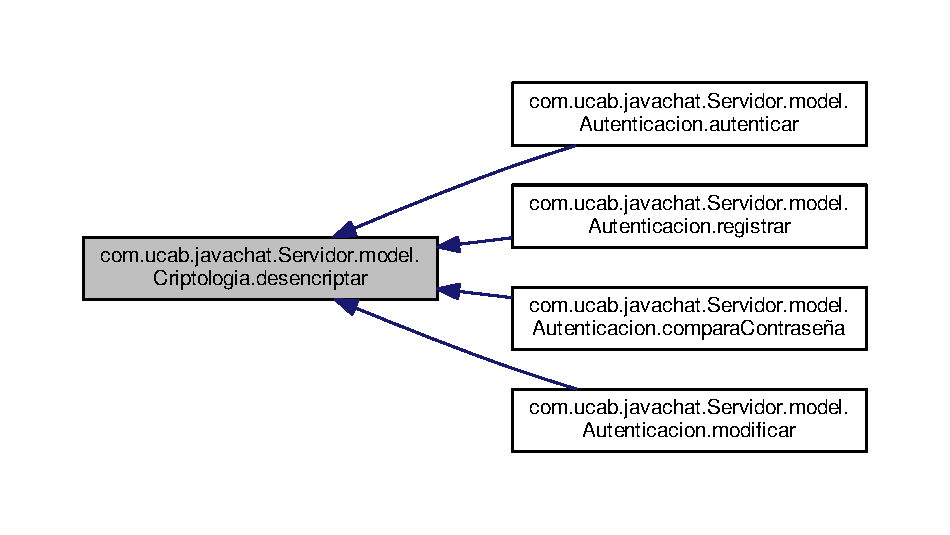
\includegraphics[width=350pt]{classcom_1_1ucab_1_1javachat_1_1_servidor_1_1model_1_1_criptologia_ae580b0995ce546a2e8b37c819651d240_icgraph}
\end{center}
\end{figure}


\hypertarget{classcom_1_1ucab_1_1javachat_1_1_servidor_1_1model_1_1_criptologia_a0a816425dbef403c92d0f858e6a910cd}{\index{com\-::ucab\-::javachat\-::\-Servidor\-::model\-::\-Criptologia@{com\-::ucab\-::javachat\-::\-Servidor\-::model\-::\-Criptologia}!encriptar@{encriptar}}
\index{encriptar@{encriptar}!com::ucab::javachat::Servidor::model::Criptologia@{com\-::ucab\-::javachat\-::\-Servidor\-::model\-::\-Criptologia}}
\subsubsection[{encriptar}]{\setlength{\rightskip}{0pt plus 5cm}static String com.\-ucab.\-javachat.\-Servidor.\-model.\-Criptologia.\-encriptar (
\begin{DoxyParamCaption}
\item[{String}]{texto}
\end{DoxyParamCaption}
)\hspace{0.3cm}{\ttfamily [static]}}}\label{classcom_1_1ucab_1_1javachat_1_1_servidor_1_1model_1_1_criptologia_a0a816425dbef403c92d0f858e6a910cd}


Definición en la línea 24 del archivo Criptologia.\-java.



La documentación para esta clase fue generada a partir del siguiente fichero\-:\begin{DoxyCompactItemize}
\item 
Escritorio/\-Chat\-Morse/src/com/ucab/javachat/\-Servidor/model/\hyperlink{_servidor_2model_2_criptologia_8java}{Criptologia.\-java}\end{DoxyCompactItemize}

\hypertarget{classcom_1_1ucab_1_1javachat_1_1_servidor_1_1model_1_1_envio_correo}{\section{Referencia de la Clase com.\-ucab.\-javachat.\-Servidor.\-model.\-Envio\-Correo}
\label{classcom_1_1ucab_1_1javachat_1_1_servidor_1_1model_1_1_envio_correo}\index{com.\-ucab.\-javachat.\-Servidor.\-model.\-Envio\-Correo@{com.\-ucab.\-javachat.\-Servidor.\-model.\-Envio\-Correo}}
}


Diagrama de colaboración para com.\-ucab.\-javachat.\-Servidor.\-model.\-Envio\-Correo\-:\nopagebreak
\begin{figure}[H]
\begin{center}
\leavevmode
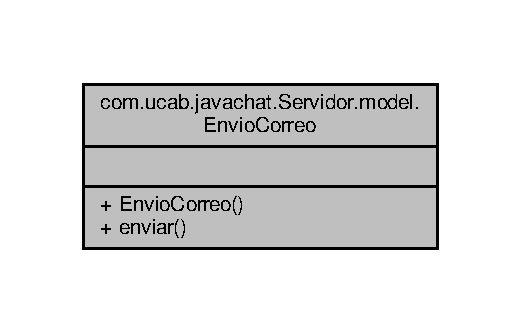
\includegraphics[width=250pt]{classcom_1_1ucab_1_1javachat_1_1_servidor_1_1model_1_1_envio_correo__coll__graph}
\end{center}
\end{figure}
\subsection*{Métodos públicos}
\begin{DoxyCompactItemize}
\item 
\hyperlink{classcom_1_1ucab_1_1javachat_1_1_servidor_1_1model_1_1_envio_correo_aba6fd1242773c58ff4d3cd57162849d6}{Envio\-Correo} (String correo, String asunto, String cuerpo)
\item 
void \hyperlink{classcom_1_1ucab_1_1javachat_1_1_servidor_1_1model_1_1_envio_correo_a0698bb7315db4d54d94ca94d95226754}{enviar} ()
\end{DoxyCompactItemize}


\subsection{Descripción detallada}


Definición en la línea 14 del archivo Envio\-Correo.\-java.



\subsection{Documentación del constructor y destructor}
\hypertarget{classcom_1_1ucab_1_1javachat_1_1_servidor_1_1model_1_1_envio_correo_aba6fd1242773c58ff4d3cd57162849d6}{\index{com\-::ucab\-::javachat\-::\-Servidor\-::model\-::\-Envio\-Correo@{com\-::ucab\-::javachat\-::\-Servidor\-::model\-::\-Envio\-Correo}!Envio\-Correo@{Envio\-Correo}}
\index{Envio\-Correo@{Envio\-Correo}!com::ucab::javachat::Servidor::model::EnvioCorreo@{com\-::ucab\-::javachat\-::\-Servidor\-::model\-::\-Envio\-Correo}}
\subsubsection[{Envio\-Correo}]{\setlength{\rightskip}{0pt plus 5cm}com.\-ucab.\-javachat.\-Servidor.\-model.\-Envio\-Correo.\-Envio\-Correo (
\begin{DoxyParamCaption}
\item[{String}]{correo, }
\item[{String}]{asunto, }
\item[{String}]{cuerpo}
\end{DoxyParamCaption}
)}}\label{classcom_1_1ucab_1_1javachat_1_1_servidor_1_1model_1_1_envio_correo_aba6fd1242773c58ff4d3cd57162849d6}


Definición en la línea 19 del archivo Envio\-Correo.\-java.



\subsection{Documentación de las funciones miembro}
\hypertarget{classcom_1_1ucab_1_1javachat_1_1_servidor_1_1model_1_1_envio_correo_a0698bb7315db4d54d94ca94d95226754}{\index{com\-::ucab\-::javachat\-::\-Servidor\-::model\-::\-Envio\-Correo@{com\-::ucab\-::javachat\-::\-Servidor\-::model\-::\-Envio\-Correo}!enviar@{enviar}}
\index{enviar@{enviar}!com::ucab::javachat::Servidor::model::EnvioCorreo@{com\-::ucab\-::javachat\-::\-Servidor\-::model\-::\-Envio\-Correo}}
\subsubsection[{enviar}]{\setlength{\rightskip}{0pt plus 5cm}void com.\-ucab.\-javachat.\-Servidor.\-model.\-Envio\-Correo.\-enviar (
\begin{DoxyParamCaption}
{}
\end{DoxyParamCaption}
)}}\label{classcom_1_1ucab_1_1javachat_1_1_servidor_1_1model_1_1_envio_correo_a0698bb7315db4d54d94ca94d95226754}


Definición en la línea 25 del archivo Envio\-Correo.\-java.



La documentación para esta clase fue generada a partir del siguiente fichero\-:\begin{DoxyCompactItemize}
\item 
Escritorio/\-Chat\-Morse/src/com/ucab/javachat/\-Servidor/model/\hyperlink{_envio_correo_8java}{Envio\-Correo.\-java}\end{DoxyCompactItemize}

\hypertarget{classcom_1_1ucab_1_1javachat_1_1_cliente_1_1model_1_1_historial}{\section{Referencia de la Clase com.\-ucab.\-javachat.\-Cliente.\-model.\-Historial}
\label{classcom_1_1ucab_1_1javachat_1_1_cliente_1_1model_1_1_historial}\index{com.\-ucab.\-javachat.\-Cliente.\-model.\-Historial@{com.\-ucab.\-javachat.\-Cliente.\-model.\-Historial}}
}


Diagrama de colaboración para com.\-ucab.\-javachat.\-Cliente.\-model.\-Historial\-:
\nopagebreak
\begin{figure}[H]
\begin{center}
\leavevmode
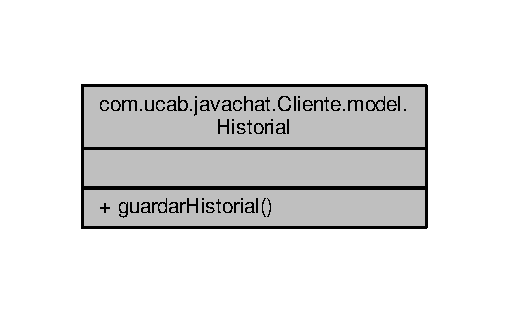
\includegraphics[width=244pt]{d5/d81/classcom_1_1ucab_1_1javachat_1_1_cliente_1_1model_1_1_historial__coll__graph}
\end{center}
\end{figure}
\subsection*{Métodos públicos estáticos}
\begin{DoxyCompactItemize}
\item 
static void \hyperlink{classcom_1_1ucab_1_1javachat_1_1_cliente_1_1model_1_1_historial_a725a59214e66a362a82a05a7b37cfb48}{guardar\-Historial} (String participantes, String texto)  throws U\-R\-I\-Syntax\-Exception, I\-O\-Exception 
\end{DoxyCompactItemize}


\subsection{Descripción detallada}
esta clase se encarga de guardar el historial de las conversaciones de el usuario \begin{DoxyAuthor}{Autor}
Grupo 3 -\/ A. Rodriguez, I. Teixeira, L. Valladares, D. Suarez 
\end{DoxyAuthor}


Definición en la línea 15 del archivo Historial.\-java.



\subsection{Documentación de las funciones miembro}
\hypertarget{classcom_1_1ucab_1_1javachat_1_1_cliente_1_1model_1_1_historial_a725a59214e66a362a82a05a7b37cfb48}{\index{com\-::ucab\-::javachat\-::\-Cliente\-::model\-::\-Historial@{com\-::ucab\-::javachat\-::\-Cliente\-::model\-::\-Historial}!guardar\-Historial@{guardar\-Historial}}
\index{guardar\-Historial@{guardar\-Historial}!com::ucab::javachat::Cliente::model::Historial@{com\-::ucab\-::javachat\-::\-Cliente\-::model\-::\-Historial}}
\subsubsection[{guardar\-Historial}]{\setlength{\rightskip}{0pt plus 5cm}static void com.\-ucab.\-javachat.\-Cliente.\-model.\-Historial.\-guardar\-Historial (
\begin{DoxyParamCaption}
\item[{String}]{participantes, }
\item[{String}]{texto}
\end{DoxyParamCaption}
) throws U\-R\-I\-Syntax\-Exception, I\-O\-Exception\hspace{0.3cm}{\ttfamily [static]}}}\label{classcom_1_1ucab_1_1javachat_1_1_cliente_1_1model_1_1_historial_a725a59214e66a362a82a05a7b37cfb48}
Crea un archivo con el nombre de los participantes de la conversación en el cual almacenara lo escrito si el archivo o directorio no existe lo crea, si existe le agrega los nuevos datos sin borrar los viejos 
\begin{DoxyParams}{Parámetros}
{\em participantes} & -\/ los participantes de la conversación \\
\hline
{\em texto} & -\/ todo el texto enviado durante esta sesion \\
\hline
\end{DoxyParams}

\begin{DoxyExceptions}{Excepciones}
{\em U\-R\-I\-Syntax\-Exception} & \\
\hline
{\em I\-O\-Exception} & \\
\hline
\end{DoxyExceptions}


Definición en la línea 26 del archivo Historial.\-java.



La documentación para esta clase fue generada a partir del siguiente fichero\-:\begin{DoxyCompactItemize}
\item 
Chat-\/\-Codigo-\/\-Morse/\-Chat\-Morse/src/com/ucab/javachat/\-Cliente/model/Historial.\-java\end{DoxyCompactItemize}

\hypertarget{classcom_1_1ucab_1_1javachat_1_1_servidor_1_1model_1_1_manejo_archivos}{\section{Referencia de la Clase com.\-ucab.\-javachat.\-Servidor.\-model.\-Manejo\-Archivos}
\label{classcom_1_1ucab_1_1javachat_1_1_servidor_1_1model_1_1_manejo_archivos}\index{com.\-ucab.\-javachat.\-Servidor.\-model.\-Manejo\-Archivos@{com.\-ucab.\-javachat.\-Servidor.\-model.\-Manejo\-Archivos}}
}


Diagrama de colaboración para com.\-ucab.\-javachat.\-Servidor.\-model.\-Manejo\-Archivos\-:\nopagebreak
\begin{figure}[H]
\begin{center}
\leavevmode
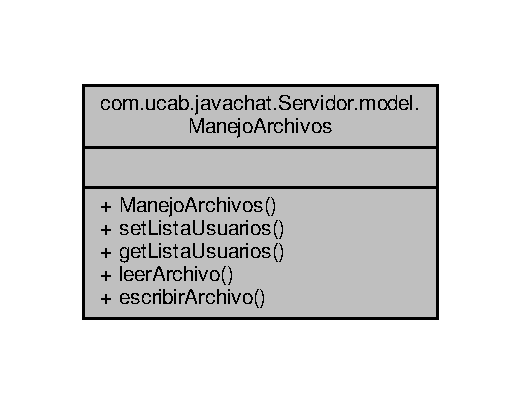
\includegraphics[width=250pt]{classcom_1_1ucab_1_1javachat_1_1_servidor_1_1model_1_1_manejo_archivos__coll__graph}
\end{center}
\end{figure}
\subsection*{Métodos públicos}
\begin{DoxyCompactItemize}
\item 
\hyperlink{classcom_1_1ucab_1_1javachat_1_1_servidor_1_1model_1_1_manejo_archivos_a61dcba785a704949bc4b84a87a223463}{Manejo\-Archivos} ()
\item 
void \hyperlink{classcom_1_1ucab_1_1javachat_1_1_servidor_1_1model_1_1_manejo_archivos_a5776d41af3206be2ef21722c54581bdb}{set\-Lista\-Usuarios} ()
\item 
Array\-List$<$ \hyperlink{classcom_1_1ucab_1_1javachat_1_1_servidor_1_1model_1_1_usuario}{Usuario} $>$ \hyperlink{classcom_1_1ucab_1_1javachat_1_1_servidor_1_1model_1_1_manejo_archivos_a659469300b3d725e66d26460107200b6}{get\-Lista\-Usuarios} ()
\item 
Array\-List$<$ \hyperlink{classcom_1_1ucab_1_1javachat_1_1_servidor_1_1model_1_1_usuario}{Usuario} $>$ \hyperlink{classcom_1_1ucab_1_1javachat_1_1_servidor_1_1model_1_1_manejo_archivos_ad6301dc8f0af55ea43b53da2c7f8b0d3}{leer\-Archivo} ()
\item 
void \hyperlink{classcom_1_1ucab_1_1javachat_1_1_servidor_1_1model_1_1_manejo_archivos_af83311d7a6185ca621aad886e6633abd}{escribir\-Archivo} (Array\-List$<$ \hyperlink{classcom_1_1ucab_1_1javachat_1_1_servidor_1_1model_1_1_usuario}{Usuario} $>$ lista\-Usuarios)
\end{DoxyCompactItemize}


\subsection{Descripción detallada}
Clase que manipula los archivos Json, el guardado y lectura de archivo y cualquier proceso relacionado

\begin{DoxyAuthor}{Autor}
Luis Valladares 
\end{DoxyAuthor}


Definición en la línea 21 del archivo Manejo\-Archivos.\-java.



\subsection{Documentación del constructor y destructor}
\hypertarget{classcom_1_1ucab_1_1javachat_1_1_servidor_1_1model_1_1_manejo_archivos_a61dcba785a704949bc4b84a87a223463}{\index{com\-::ucab\-::javachat\-::\-Servidor\-::model\-::\-Manejo\-Archivos@{com\-::ucab\-::javachat\-::\-Servidor\-::model\-::\-Manejo\-Archivos}!Manejo\-Archivos@{Manejo\-Archivos}}
\index{Manejo\-Archivos@{Manejo\-Archivos}!com::ucab::javachat::Servidor::model::ManejoArchivos@{com\-::ucab\-::javachat\-::\-Servidor\-::model\-::\-Manejo\-Archivos}}
\subsubsection[{Manejo\-Archivos}]{\setlength{\rightskip}{0pt plus 5cm}com.\-ucab.\-javachat.\-Servidor.\-model.\-Manejo\-Archivos.\-Manejo\-Archivos (
\begin{DoxyParamCaption}
{}
\end{DoxyParamCaption}
)}}\label{classcom_1_1ucab_1_1javachat_1_1_servidor_1_1model_1_1_manejo_archivos_a61dcba785a704949bc4b84a87a223463}


Definición en la línea 31 del archivo Manejo\-Archivos.\-java.



Gráfico de llamadas para esta función\-:\nopagebreak
\begin{figure}[H]
\begin{center}
\leavevmode
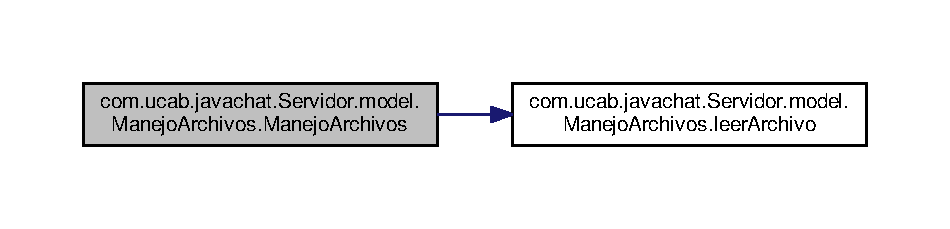
\includegraphics[width=350pt]{classcom_1_1ucab_1_1javachat_1_1_servidor_1_1model_1_1_manejo_archivos_a61dcba785a704949bc4b84a87a223463_cgraph}
\end{center}
\end{figure}




\subsection{Documentación de las funciones miembro}
\hypertarget{classcom_1_1ucab_1_1javachat_1_1_servidor_1_1model_1_1_manejo_archivos_af83311d7a6185ca621aad886e6633abd}{\index{com\-::ucab\-::javachat\-::\-Servidor\-::model\-::\-Manejo\-Archivos@{com\-::ucab\-::javachat\-::\-Servidor\-::model\-::\-Manejo\-Archivos}!escribir\-Archivo@{escribir\-Archivo}}
\index{escribir\-Archivo@{escribir\-Archivo}!com::ucab::javachat::Servidor::model::ManejoArchivos@{com\-::ucab\-::javachat\-::\-Servidor\-::model\-::\-Manejo\-Archivos}}
\subsubsection[{escribir\-Archivo}]{\setlength{\rightskip}{0pt plus 5cm}void com.\-ucab.\-javachat.\-Servidor.\-model.\-Manejo\-Archivos.\-escribir\-Archivo (
\begin{DoxyParamCaption}
\item[{Array\-List$<$ {\bf Usuario} $>$}]{lista\-Usuarios}
\end{DoxyParamCaption}
)}}\label{classcom_1_1ucab_1_1javachat_1_1_servidor_1_1model_1_1_manejo_archivos_af83311d7a6185ca621aad886e6633abd}
Almacena los datos que se encuentran en la lista pasada a un archivo Json \begin{DoxyAuthor}{Autor}
Luis Valladares 
\end{DoxyAuthor}

\begin{DoxyParams}{Parámetros}
{\em Lista} & de usuarios a guardar \\
\hline
\end{DoxyParams}


Definición en la línea 83 del archivo Manejo\-Archivos.\-java.

\hypertarget{classcom_1_1ucab_1_1javachat_1_1_servidor_1_1model_1_1_manejo_archivos_a659469300b3d725e66d26460107200b6}{\index{com\-::ucab\-::javachat\-::\-Servidor\-::model\-::\-Manejo\-Archivos@{com\-::ucab\-::javachat\-::\-Servidor\-::model\-::\-Manejo\-Archivos}!get\-Lista\-Usuarios@{get\-Lista\-Usuarios}}
\index{get\-Lista\-Usuarios@{get\-Lista\-Usuarios}!com::ucab::javachat::Servidor::model::ManejoArchivos@{com\-::ucab\-::javachat\-::\-Servidor\-::model\-::\-Manejo\-Archivos}}
\subsubsection[{get\-Lista\-Usuarios}]{\setlength{\rightskip}{0pt plus 5cm}Array\-List$<${\bf Usuario}$>$ com.\-ucab.\-javachat.\-Servidor.\-model.\-Manejo\-Archivos.\-get\-Lista\-Usuarios (
\begin{DoxyParamCaption}
{}
\end{DoxyParamCaption}
)}}\label{classcom_1_1ucab_1_1javachat_1_1_servidor_1_1model_1_1_manejo_archivos_a659469300b3d725e66d26460107200b6}
\begin{DoxyReturn}{Devuelve}

\end{DoxyReturn}


Definición en la línea 51 del archivo Manejo\-Archivos.\-java.



Gráfico de llamadas a esta función\-:\nopagebreak
\begin{figure}[H]
\begin{center}
\leavevmode
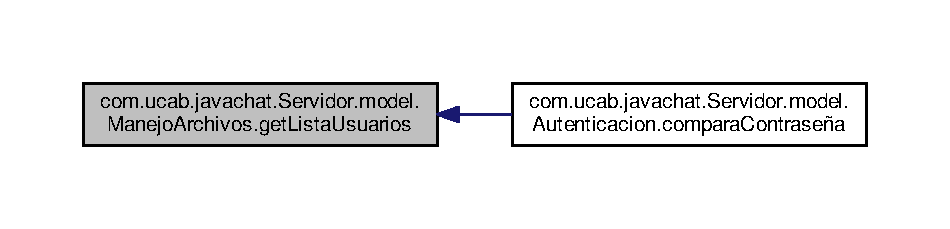
\includegraphics[width=350pt]{classcom_1_1ucab_1_1javachat_1_1_servidor_1_1model_1_1_manejo_archivos_a659469300b3d725e66d26460107200b6_icgraph}
\end{center}
\end{figure}


\hypertarget{classcom_1_1ucab_1_1javachat_1_1_servidor_1_1model_1_1_manejo_archivos_ad6301dc8f0af55ea43b53da2c7f8b0d3}{\index{com\-::ucab\-::javachat\-::\-Servidor\-::model\-::\-Manejo\-Archivos@{com\-::ucab\-::javachat\-::\-Servidor\-::model\-::\-Manejo\-Archivos}!leer\-Archivo@{leer\-Archivo}}
\index{leer\-Archivo@{leer\-Archivo}!com::ucab::javachat::Servidor::model::ManejoArchivos@{com\-::ucab\-::javachat\-::\-Servidor\-::model\-::\-Manejo\-Archivos}}
\subsubsection[{leer\-Archivo}]{\setlength{\rightskip}{0pt plus 5cm}Array\-List$<${\bf Usuario}$>$ com.\-ucab.\-javachat.\-Servidor.\-model.\-Manejo\-Archivos.\-leer\-Archivo (
\begin{DoxyParamCaption}
{}
\end{DoxyParamCaption}
)}}\label{classcom_1_1ucab_1_1javachat_1_1_servidor_1_1model_1_1_manejo_archivos_ad6301dc8f0af55ea43b53da2c7f8b0d3}
Lee los datos de un archivo json en una ruta previamente establecida luego de que lo extrae, lo almacena en un Array\-List de tipo usuario que tendra a todos los usuarios del sistemas

\begin{DoxyReturn}{Devuelve}
La lista de usuarios 
\end{DoxyReturn}
\begin{DoxyAuthor}{Autor}
Luis Valladares 
\end{DoxyAuthor}


Definición en la línea 63 del archivo Manejo\-Archivos.\-java.



Gráfico de llamadas a esta función\-:\nopagebreak
\begin{figure}[H]
\begin{center}
\leavevmode
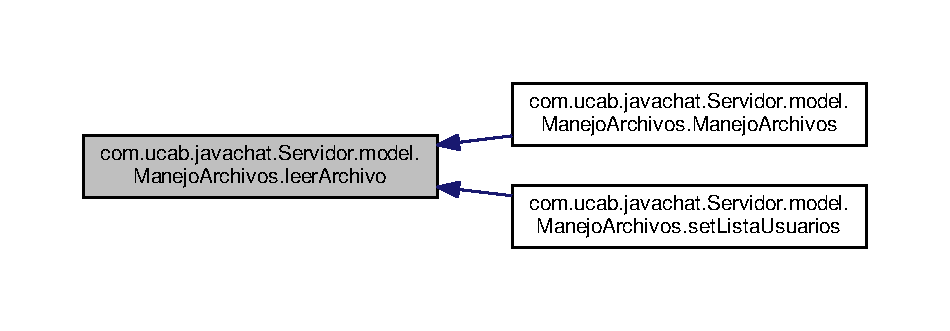
\includegraphics[width=350pt]{classcom_1_1ucab_1_1javachat_1_1_servidor_1_1model_1_1_manejo_archivos_ad6301dc8f0af55ea43b53da2c7f8b0d3_icgraph}
\end{center}
\end{figure}


\hypertarget{classcom_1_1ucab_1_1javachat_1_1_servidor_1_1model_1_1_manejo_archivos_a5776d41af3206be2ef21722c54581bdb}{\index{com\-::ucab\-::javachat\-::\-Servidor\-::model\-::\-Manejo\-Archivos@{com\-::ucab\-::javachat\-::\-Servidor\-::model\-::\-Manejo\-Archivos}!set\-Lista\-Usuarios@{set\-Lista\-Usuarios}}
\index{set\-Lista\-Usuarios@{set\-Lista\-Usuarios}!com::ucab::javachat::Servidor::model::ManejoArchivos@{com\-::ucab\-::javachat\-::\-Servidor\-::model\-::\-Manejo\-Archivos}}
\subsubsection[{set\-Lista\-Usuarios}]{\setlength{\rightskip}{0pt plus 5cm}void com.\-ucab.\-javachat.\-Servidor.\-model.\-Manejo\-Archivos.\-set\-Lista\-Usuarios (
\begin{DoxyParamCaption}
{}
\end{DoxyParamCaption}
)}}\label{classcom_1_1ucab_1_1javachat_1_1_servidor_1_1model_1_1_manejo_archivos_a5776d41af3206be2ef21722c54581bdb}


Definición en la línea 44 del archivo Manejo\-Archivos.\-java.



Gráfico de llamadas para esta función\-:\nopagebreak
\begin{figure}[H]
\begin{center}
\leavevmode
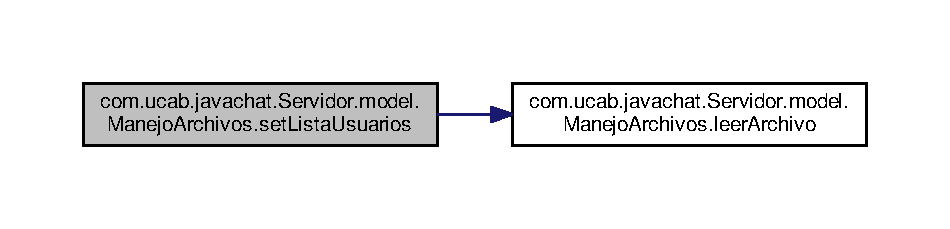
\includegraphics[width=350pt]{classcom_1_1ucab_1_1javachat_1_1_servidor_1_1model_1_1_manejo_archivos_a5776d41af3206be2ef21722c54581bdb_cgraph}
\end{center}
\end{figure}




La documentación para esta clase fue generada a partir del siguiente fichero\-:\begin{DoxyCompactItemize}
\item 
Escritorio/\-Chat\-Morse/src/com/ucab/javachat/\-Servidor/model/\hyperlink{_manejo_archivos_8java}{Manejo\-Archivos.\-java}\end{DoxyCompactItemize}

\hypertarget{classcom_1_1ucab_1_1javachat_1_1_servidor_1_1main_1_1_principal}{\section{Referencia de la Clase com.\-ucab.\-javachat.\-Servidor.\-main.\-Principal}
\label{classcom_1_1ucab_1_1javachat_1_1_servidor_1_1main_1_1_principal}\index{com.\-ucab.\-javachat.\-Servidor.\-main.\-Principal@{com.\-ucab.\-javachat.\-Servidor.\-main.\-Principal}}
}


Diagrama de colaboración para com.\-ucab.\-javachat.\-Servidor.\-main.\-Principal\-:
\nopagebreak
\begin{figure}[H]
\begin{center}
\leavevmode
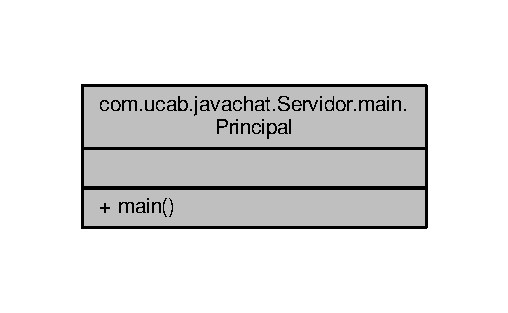
\includegraphics[width=244pt]{de/d41/classcom_1_1ucab_1_1javachat_1_1_servidor_1_1main_1_1_principal__coll__graph}
\end{center}
\end{figure}
\subsection*{Métodos públicos estáticos}
\begin{DoxyCompactItemize}
\item 
\hypertarget{classcom_1_1ucab_1_1javachat_1_1_servidor_1_1main_1_1_principal_aab5df0d2fa877ce007a67fa8be56df79}{static void {\bfseries main} (String abc\mbox{[}$\,$\mbox{]})  throws I\-O\-Exception 	   }\label{classcom_1_1ucab_1_1javachat_1_1_servidor_1_1main_1_1_principal_aab5df0d2fa877ce007a67fa8be56df79}

\end{DoxyCompactItemize}


\subsection{Descripción detallada}


Definición en la línea 12 del archivo Principal.\-java.



La documentación para esta clase fue generada a partir del siguiente fichero\-:\begin{DoxyCompactItemize}
\item 
Chat-\/\-Codigo-\/\-Morse/\-Chat\-Morse/src/com/ucab/javachat/\-Servidor/main/Principal.\-java\end{DoxyCompactItemize}

\hypertarget{classcom_1_1ucab_1_1javachat_1_1_cliente_1_1main_1_1_principal}{\section{Referencia de la Clase com.\-ucab.\-javachat.\-Cliente.\-main.\-Principal}
\label{classcom_1_1ucab_1_1javachat_1_1_cliente_1_1main_1_1_principal}\index{com.\-ucab.\-javachat.\-Cliente.\-main.\-Principal@{com.\-ucab.\-javachat.\-Cliente.\-main.\-Principal}}
}


Diagrama de colaboración para com.\-ucab.\-javachat.\-Cliente.\-main.\-Principal\-:\nopagebreak
\begin{figure}[H]
\begin{center}
\leavevmode
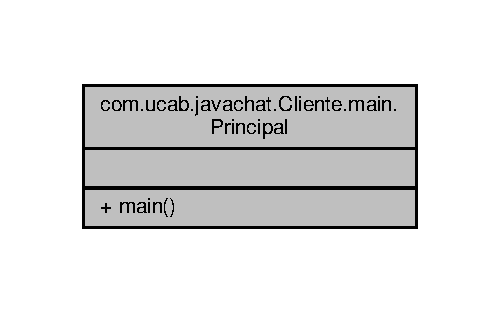
\includegraphics[width=240pt]{classcom_1_1ucab_1_1javachat_1_1_cliente_1_1main_1_1_principal__coll__graph}
\end{center}
\end{figure}
\subsection*{Métodos públicos estáticos}
\begin{DoxyCompactItemize}
\item 
static void \hyperlink{classcom_1_1ucab_1_1javachat_1_1_cliente_1_1main_1_1_principal_a0560b184945ff743d2f7a9225b2a8e12}{main} (String args\mbox{[}$\,$\mbox{]})  throws I\-O\-Exception 
\end{DoxyCompactItemize}


\subsection{Descripción detallada}


Definición en la línea 9 del archivo Principal.\-java.



\subsection{Documentación de las funciones miembro}
\hypertarget{classcom_1_1ucab_1_1javachat_1_1_cliente_1_1main_1_1_principal_a0560b184945ff743d2f7a9225b2a8e12}{\index{com\-::ucab\-::javachat\-::\-Cliente\-::main\-::\-Principal@{com\-::ucab\-::javachat\-::\-Cliente\-::main\-::\-Principal}!main@{main}}
\index{main@{main}!com::ucab::javachat::Cliente::main::Principal@{com\-::ucab\-::javachat\-::\-Cliente\-::main\-::\-Principal}}
\subsubsection[{main}]{\setlength{\rightskip}{0pt plus 5cm}static void com.\-ucab.\-javachat.\-Cliente.\-main.\-Principal.\-main (
\begin{DoxyParamCaption}
\item[{String}]{args\mbox{[}$\,$\mbox{]}}
\end{DoxyParamCaption}
) throws I\-O\-Exception\hspace{0.3cm}{\ttfamily [static]}}}\label{classcom_1_1ucab_1_1javachat_1_1_cliente_1_1main_1_1_principal_a0560b184945ff743d2f7a9225b2a8e12}


Definición en la línea 11 del archivo Principal.\-java.



La documentación para esta clase fue generada a partir del siguiente fichero\-:\begin{DoxyCompactItemize}
\item 
Escritorio/\-Chat\-Morse/src/com/ucab/javachat/\-Cliente/main/\hyperlink{_cliente_2main_2_principal_8java}{Principal.\-java}\end{DoxyCompactItemize}

\hypertarget{classcom_1_1ucab_1_1javachat_1_1_cliente_1_1model_1_1_reproducir_sonido}{\section{Referencia de la Clase com.\-ucab.\-javachat.\-Cliente.\-model.\-Reproducir\-Sonido}
\label{classcom_1_1ucab_1_1javachat_1_1_cliente_1_1model_1_1_reproducir_sonido}\index{com.\-ucab.\-javachat.\-Cliente.\-model.\-Reproducir\-Sonido@{com.\-ucab.\-javachat.\-Cliente.\-model.\-Reproducir\-Sonido}}
}


Diagrama de herencias de com.\-ucab.\-javachat.\-Cliente.\-model.\-Reproducir\-Sonido
\nopagebreak
\begin{figure}[H]
\begin{center}
\leavevmode
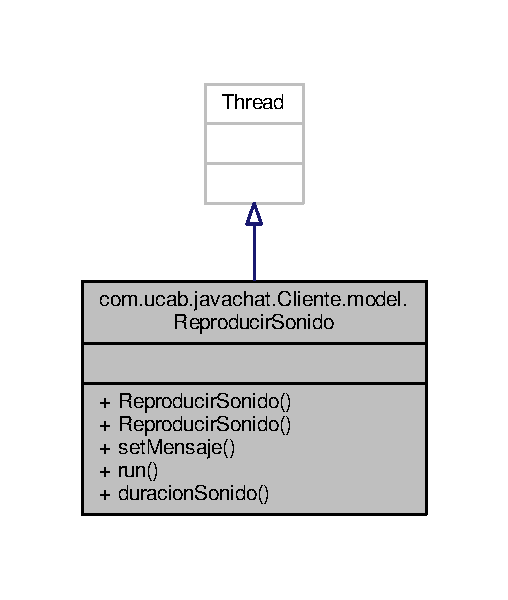
\includegraphics[width=244pt]{d7/d0d/classcom_1_1ucab_1_1javachat_1_1_cliente_1_1model_1_1_reproducir_sonido__inherit__graph}
\end{center}
\end{figure}


Diagrama de colaboración para com.\-ucab.\-javachat.\-Cliente.\-model.\-Reproducir\-Sonido\-:
\nopagebreak
\begin{figure}[H]
\begin{center}
\leavevmode
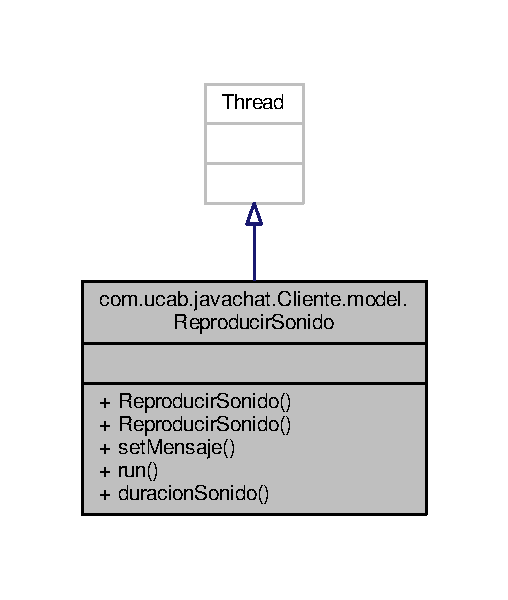
\includegraphics[width=244pt]{d4/d5e/classcom_1_1ucab_1_1javachat_1_1_cliente_1_1model_1_1_reproducir_sonido__coll__graph}
\end{center}
\end{figure}
\subsection*{Métodos públicos}
\begin{DoxyCompactItemize}
\item 
\hyperlink{classcom_1_1ucab_1_1javachat_1_1_cliente_1_1model_1_1_reproducir_sonido_ac10d27e817edf62839046eb5f07aa236}{Reproducir\-Sonido} ()
\item 
\hypertarget{classcom_1_1ucab_1_1javachat_1_1_cliente_1_1model_1_1_reproducir_sonido_aaed28ce271a5d5a7975ef77c8ae26274}{{\bfseries Reproducir\-Sonido} (String mensaje)}\label{classcom_1_1ucab_1_1javachat_1_1_cliente_1_1model_1_1_reproducir_sonido_aaed28ce271a5d5a7975ef77c8ae26274}

\item 
void \hyperlink{classcom_1_1ucab_1_1javachat_1_1_cliente_1_1model_1_1_reproducir_sonido_a00ae7bbb07322bf4d4b578c0d10b34bb}{set\-Mensaje} (String mensaje)
\item 
void \hyperlink{classcom_1_1ucab_1_1javachat_1_1_cliente_1_1model_1_1_reproducir_sonido_ac8f472ebd53121c63b932d0264dfa917}{run} ()
\item 
long \hyperlink{classcom_1_1ucab_1_1javachat_1_1_cliente_1_1model_1_1_reproducir_sonido_aa251ecd4cbf7251b58ec572a5d3f4656}{duracion\-Sonido} ()
\end{DoxyCompactItemize}


\subsection{Descripción detallada}
Clase que se encarga de reproducir mediante sonidos de codigo morse los mensajes enviados por los usuarios. \begin{DoxyAuthor}{Autor}
Grupo 3 
\end{DoxyAuthor}


Definición en la línea 18 del archivo Reproducir\-Sonido.\-java.



\subsection{Documentación del constructor y destructor}
\hypertarget{classcom_1_1ucab_1_1javachat_1_1_cliente_1_1model_1_1_reproducir_sonido_ac10d27e817edf62839046eb5f07aa236}{\index{com\-::ucab\-::javachat\-::\-Cliente\-::model\-::\-Reproducir\-Sonido@{com\-::ucab\-::javachat\-::\-Cliente\-::model\-::\-Reproducir\-Sonido}!Reproducir\-Sonido@{Reproducir\-Sonido}}
\index{Reproducir\-Sonido@{Reproducir\-Sonido}!com::ucab::javachat::Cliente::model::ReproducirSonido@{com\-::ucab\-::javachat\-::\-Cliente\-::model\-::\-Reproducir\-Sonido}}
\subsubsection[{Reproducir\-Sonido}]{\setlength{\rightskip}{0pt plus 5cm}com.\-ucab.\-javachat.\-Cliente.\-model.\-Reproducir\-Sonido.\-Reproducir\-Sonido (
\begin{DoxyParamCaption}
{}
\end{DoxyParamCaption}
)}}\label{classcom_1_1ucab_1_1javachat_1_1_cliente_1_1model_1_1_reproducir_sonido_ac10d27e817edf62839046eb5f07aa236}
Constructores con y sin parametros 

Definición en la línea 24 del archivo Reproducir\-Sonido.\-java.



\subsection{Documentación de las funciones miembro}
\hypertarget{classcom_1_1ucab_1_1javachat_1_1_cliente_1_1model_1_1_reproducir_sonido_aa251ecd4cbf7251b58ec572a5d3f4656}{\index{com\-::ucab\-::javachat\-::\-Cliente\-::model\-::\-Reproducir\-Sonido@{com\-::ucab\-::javachat\-::\-Cliente\-::model\-::\-Reproducir\-Sonido}!duracion\-Sonido@{duracion\-Sonido}}
\index{duracion\-Sonido@{duracion\-Sonido}!com::ucab::javachat::Cliente::model::ReproducirSonido@{com\-::ucab\-::javachat\-::\-Cliente\-::model\-::\-Reproducir\-Sonido}}
\subsubsection[{duracion\-Sonido}]{\setlength{\rightskip}{0pt plus 5cm}long com.\-ucab.\-javachat.\-Cliente.\-model.\-Reproducir\-Sonido.\-duracion\-Sonido (
\begin{DoxyParamCaption}
{}
\end{DoxyParamCaption}
)}}\label{classcom_1_1ucab_1_1javachat_1_1_cliente_1_1model_1_1_reproducir_sonido_aa251ecd4cbf7251b58ec572a5d3f4656}
Metodo que se encarga del espacio de sonido que hay entre cada caracter del mensaje \begin{DoxyReturn}{Devuelve}
duracion 
\end{DoxyReturn}


Definición en la línea 140 del archivo Reproducir\-Sonido.\-java.

\hypertarget{classcom_1_1ucab_1_1javachat_1_1_cliente_1_1model_1_1_reproducir_sonido_ac8f472ebd53121c63b932d0264dfa917}{\index{com\-::ucab\-::javachat\-::\-Cliente\-::model\-::\-Reproducir\-Sonido@{com\-::ucab\-::javachat\-::\-Cliente\-::model\-::\-Reproducir\-Sonido}!run@{run}}
\index{run@{run}!com::ucab::javachat::Cliente::model::ReproducirSonido@{com\-::ucab\-::javachat\-::\-Cliente\-::model\-::\-Reproducir\-Sonido}}
\subsubsection[{run}]{\setlength{\rightskip}{0pt plus 5cm}void com.\-ucab.\-javachat.\-Cliente.\-model.\-Reproducir\-Sonido.\-run (
\begin{DoxyParamCaption}
{}
\end{DoxyParamCaption}
)}}\label{classcom_1_1ucab_1_1javachat_1_1_cliente_1_1model_1_1_reproducir_sonido_ac8f472ebd53121c63b932d0264dfa917}
Implementacioon del metodo run. en este metodo se debe implementar la funcionalidad de la clase. Se implementa en este metodo porque hereda de la clase Thread. 

Definición en la línea 40 del archivo Reproducir\-Sonido.\-java.

\hypertarget{classcom_1_1ucab_1_1javachat_1_1_cliente_1_1model_1_1_reproducir_sonido_a00ae7bbb07322bf4d4b578c0d10b34bb}{\index{com\-::ucab\-::javachat\-::\-Cliente\-::model\-::\-Reproducir\-Sonido@{com\-::ucab\-::javachat\-::\-Cliente\-::model\-::\-Reproducir\-Sonido}!set\-Mensaje@{set\-Mensaje}}
\index{set\-Mensaje@{set\-Mensaje}!com::ucab::javachat::Cliente::model::ReproducirSonido@{com\-::ucab\-::javachat\-::\-Cliente\-::model\-::\-Reproducir\-Sonido}}
\subsubsection[{set\-Mensaje}]{\setlength{\rightskip}{0pt plus 5cm}void com.\-ucab.\-javachat.\-Cliente.\-model.\-Reproducir\-Sonido.\-set\-Mensaje (
\begin{DoxyParamCaption}
\item[{String}]{mensaje}
\end{DoxyParamCaption}
)}}\label{classcom_1_1ucab_1_1javachat_1_1_cliente_1_1model_1_1_reproducir_sonido_a00ae7bbb07322bf4d4b578c0d10b34bb}
Setter para ek mensaje que se reproducira 
\begin{DoxyParams}{Parámetros}
{\em mensaje} & \\
\hline
\end{DoxyParams}


Definición en la línea 33 del archivo Reproducir\-Sonido.\-java.



La documentación para esta clase fue generada a partir del siguiente fichero\-:\begin{DoxyCompactItemize}
\item 
Chat-\/\-Codigo-\/\-Morse/\-Chat\-Morse/src/com/ucab/javachat/\-Cliente/model/Reproducir\-Sonido.\-java\end{DoxyCompactItemize}

\hypertarget{classcom_1_1ucab_1_1javachat_1_1_servidor_1_1controller_1_1_servidor_controller}{\section{Referencia de la Clase com.\-ucab.\-javachat.\-Servidor.\-controller.\-Servidor\-Controller}
\label{classcom_1_1ucab_1_1javachat_1_1_servidor_1_1controller_1_1_servidor_controller}\index{com.\-ucab.\-javachat.\-Servidor.\-controller.\-Servidor\-Controller@{com.\-ucab.\-javachat.\-Servidor.\-controller.\-Servidor\-Controller}}
}


Diagrama de colaboración para com.\-ucab.\-javachat.\-Servidor.\-controller.\-Servidor\-Controller\-:
\nopagebreak
\begin{figure}[H]
\begin{center}
\leavevmode
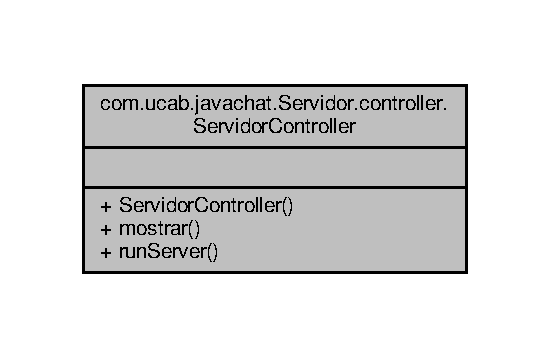
\includegraphics[width=264pt]{df/d6b/classcom_1_1ucab_1_1javachat_1_1_servidor_1_1controller_1_1_servidor_controller__coll__graph}
\end{center}
\end{figure}
\subsection*{Métodos públicos}
\begin{DoxyCompactItemize}
\item 
\hyperlink{classcom_1_1ucab_1_1javachat_1_1_servidor_1_1controller_1_1_servidor_controller_a36f238b4a06304d92f09c51ca60c31e5}{Servidor\-Controller} (\hyperlink{classcom_1_1ucab_1_1javachat_1_1_servidor_1_1view_1_1_servidor_view}{Servidor\-View} vista)
\item 
void \hyperlink{classcom_1_1ucab_1_1javachat_1_1_servidor_1_1controller_1_1_servidor_controller_a73afbbd665ab0cdb6bfb58e1726ffe3c}{mostrar} (String msg)
\item 
void \hyperlink{classcom_1_1ucab_1_1javachat_1_1_servidor_1_1controller_1_1_servidor_controller_a363c2a7d307466fc9afd04fa3de32b68}{run\-Server} ()
\end{DoxyCompactItemize}


\subsection{Descripción detallada}
Clase que controla la parte del servidor \begin{DoxyAuthor}{Autor}
Grupo 3 
\end{DoxyAuthor}


Definición en la línea 13 del archivo Servidor\-Controller.\-java.



\subsection{Documentación del constructor y destructor}
\hypertarget{classcom_1_1ucab_1_1javachat_1_1_servidor_1_1controller_1_1_servidor_controller_a36f238b4a06304d92f09c51ca60c31e5}{\index{com\-::ucab\-::javachat\-::\-Servidor\-::controller\-::\-Servidor\-Controller@{com\-::ucab\-::javachat\-::\-Servidor\-::controller\-::\-Servidor\-Controller}!Servidor\-Controller@{Servidor\-Controller}}
\index{Servidor\-Controller@{Servidor\-Controller}!com::ucab::javachat::Servidor::controller::ServidorController@{com\-::ucab\-::javachat\-::\-Servidor\-::controller\-::\-Servidor\-Controller}}
\subsubsection[{Servidor\-Controller}]{\setlength{\rightskip}{0pt plus 5cm}com.\-ucab.\-javachat.\-Servidor.\-controller.\-Servidor\-Controller.\-Servidor\-Controller (
\begin{DoxyParamCaption}
\item[{{\bf Servidor\-View}}]{vista}
\end{DoxyParamCaption}
)}}\label{classcom_1_1ucab_1_1javachat_1_1_servidor_1_1controller_1_1_servidor_controller_a36f238b4a06304d92f09c51ca60c31e5}
metodo que se encarga de iniciar la vista del servidor y llama al metodo run\-Server 
\begin{DoxyParams}{Parámetros}
{\em vista} & \\
\hline
\end{DoxyParams}


Definición en la línea 20 del archivo Servidor\-Controller.\-java.



Gráfico de llamadas para esta función\-:
\nopagebreak
\begin{figure}[H]
\begin{center}
\leavevmode
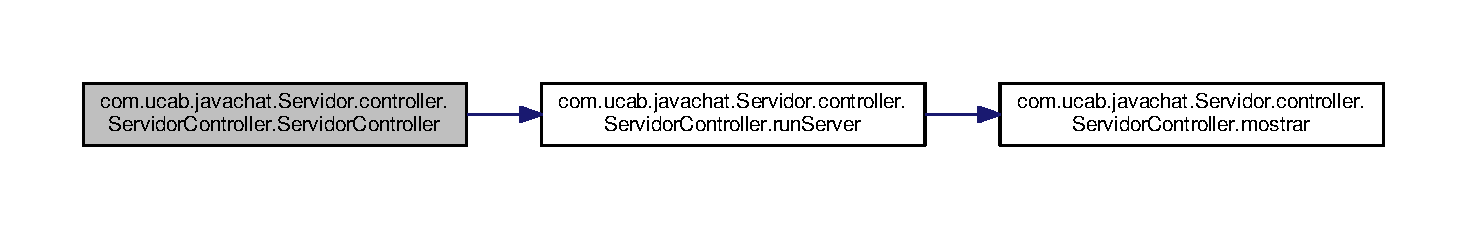
\includegraphics[width=350pt]{d8/d63/classcom_1_1ucab_1_1javachat_1_1_servidor_1_1controller_1_1_servidor_controller_a36f238b4a06304d92f09c51ca60c31e5_cgraph}
\end{center}
\end{figure}




\subsection{Documentación de las funciones miembro}
\hypertarget{classcom_1_1ucab_1_1javachat_1_1_servidor_1_1controller_1_1_servidor_controller_a73afbbd665ab0cdb6bfb58e1726ffe3c}{\index{com\-::ucab\-::javachat\-::\-Servidor\-::controller\-::\-Servidor\-Controller@{com\-::ucab\-::javachat\-::\-Servidor\-::controller\-::\-Servidor\-Controller}!mostrar@{mostrar}}
\index{mostrar@{mostrar}!com::ucab::javachat::Servidor::controller::ServidorController@{com\-::ucab\-::javachat\-::\-Servidor\-::controller\-::\-Servidor\-Controller}}
\subsubsection[{mostrar}]{\setlength{\rightskip}{0pt plus 5cm}void com.\-ucab.\-javachat.\-Servidor.\-controller.\-Servidor\-Controller.\-mostrar (
\begin{DoxyParamCaption}
\item[{String}]{msg}
\end{DoxyParamCaption}
)}}\label{classcom_1_1ucab_1_1javachat_1_1_servidor_1_1controller_1_1_servidor_controller_a73afbbd665ab0cdb6bfb58e1726ffe3c}
metodo necargado de agregar a la ventana del servidor el mensaje que recibe como parametro 
\begin{DoxyParams}{Parámetros}
{\em msg} & \\
\hline
\end{DoxyParams}


Definición en la línea 30 del archivo Servidor\-Controller.\-java.



Gráfico de llamadas a esta función\-:
\nopagebreak
\begin{figure}[H]
\begin{center}
\leavevmode
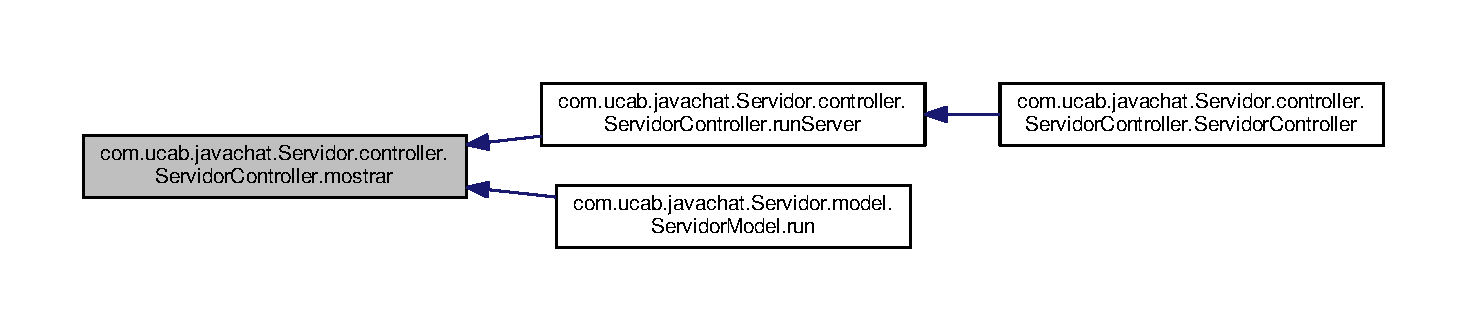
\includegraphics[width=350pt]{d8/d63/classcom_1_1ucab_1_1javachat_1_1_servidor_1_1controller_1_1_servidor_controller_a73afbbd665ab0cdb6bfb58e1726ffe3c_icgraph}
\end{center}
\end{figure}


\hypertarget{classcom_1_1ucab_1_1javachat_1_1_servidor_1_1controller_1_1_servidor_controller_a363c2a7d307466fc9afd04fa3de32b68}{\index{com\-::ucab\-::javachat\-::\-Servidor\-::controller\-::\-Servidor\-Controller@{com\-::ucab\-::javachat\-::\-Servidor\-::controller\-::\-Servidor\-Controller}!run\-Server@{run\-Server}}
\index{run\-Server@{run\-Server}!com::ucab::javachat::Servidor::controller::ServidorController@{com\-::ucab\-::javachat\-::\-Servidor\-::controller\-::\-Servidor\-Controller}}
\subsubsection[{run\-Server}]{\setlength{\rightskip}{0pt plus 5cm}void com.\-ucab.\-javachat.\-Servidor.\-controller.\-Servidor\-Controller.\-run\-Server (
\begin{DoxyParamCaption}
{}
\end{DoxyParamCaption}
)}}\label{classcom_1_1ucab_1_1javachat_1_1_servidor_1_1controller_1_1_servidor_controller_a363c2a7d307466fc9afd04fa3de32b68}
metodo encargado de inicializar los sockets y poder admitir usuarios en la aplicacion 

Definición en la línea 38 del archivo Servidor\-Controller.\-java.



Gráfico de llamadas para esta función\-:
\nopagebreak
\begin{figure}[H]
\begin{center}
\leavevmode
\includegraphics[width=350pt]{d8/d63/classcom_1_1ucab_1_1javachat_1_1_servidor_1_1controller_1_1_servidor_controller_a363c2a7d307466fc9afd04fa3de32b68_cgraph}
\end{center}
\end{figure}




Gráfico de llamadas a esta función\-:
\nopagebreak
\begin{figure}[H]
\begin{center}
\leavevmode
\includegraphics[width=350pt]{d8/d63/classcom_1_1ucab_1_1javachat_1_1_servidor_1_1controller_1_1_servidor_controller_a363c2a7d307466fc9afd04fa3de32b68_icgraph}
\end{center}
\end{figure}




La documentación para esta clase fue generada a partir del siguiente fichero\-:\begin{DoxyCompactItemize}
\item 
Chat-\/\-Codigo-\/\-Morse/\-Chat\-Morse/src/com/ucab/javachat/\-Servidor/controller/Servidor\-Controller.\-java\end{DoxyCompactItemize}

\hypertarget{classcom_1_1ucab_1_1javachat_1_1_servidor_1_1model_1_1_servidor_model}{\section{Referencia de la Clase com.\-ucab.\-javachat.\-Servidor.\-model.\-Servidor\-Model}
\label{classcom_1_1ucab_1_1javachat_1_1_servidor_1_1model_1_1_servidor_model}\index{com.\-ucab.\-javachat.\-Servidor.\-model.\-Servidor\-Model@{com.\-ucab.\-javachat.\-Servidor.\-model.\-Servidor\-Model}}
}


Diagrama de herencias de com.\-ucab.\-javachat.\-Servidor.\-model.\-Servidor\-Model
\nopagebreak
\begin{figure}[H]
\begin{center}
\leavevmode
\includegraphics[width=250pt]{da/d11/classcom_1_1ucab_1_1javachat_1_1_servidor_1_1model_1_1_servidor_model__inherit__graph}
\end{center}
\end{figure}


Diagrama de colaboración para com.\-ucab.\-javachat.\-Servidor.\-model.\-Servidor\-Model\-:
\nopagebreak
\begin{figure}[H]
\begin{center}
\leavevmode
\includegraphics[width=350pt]{de/d22/classcom_1_1ucab_1_1javachat_1_1_servidor_1_1model_1_1_servidor_model__coll__graph}
\end{center}
\end{figure}
\subsection*{Métodos públicos}
\begin{DoxyCompactItemize}
\item 
\hyperlink{classcom_1_1ucab_1_1javachat_1_1_servidor_1_1model_1_1_servidor_model_aa0ce2b6483d9538d362f45e2ff7e7263}{Servidor\-Model} (Socket scliente, Socket scliente2, \hyperlink{classcom_1_1ucab_1_1javachat_1_1_servidor_1_1controller_1_1_servidor_controller}{Servidor\-Controller} serv)
\item 
void \hyperlink{classcom_1_1ucab_1_1javachat_1_1_servidor_1_1model_1_1_servidor_model_a21f82e0d41c53cb292a639e580e5eb59}{set\-Name\-User} (String user)
\item 
\hypertarget{classcom_1_1ucab_1_1javachat_1_1_servidor_1_1model_1_1_servidor_model_aad88766777b8f162d8ee92ba5de47fee}{String {\bfseries get\-Name\-User} ()}\label{classcom_1_1ucab_1_1javachat_1_1_servidor_1_1model_1_1_servidor_model_aad88766777b8f162d8ee92ba5de47fee}

\item 
\hypertarget{classcom_1_1ucab_1_1javachat_1_1_servidor_1_1model_1_1_servidor_model_a72058125b761c7703bad54a8bec5c25a}{void {\bfseries set\-Clave} (String clave)}\label{classcom_1_1ucab_1_1javachat_1_1_servidor_1_1model_1_1_servidor_model_a72058125b761c7703bad54a8bec5c25a}

\item 
\hypertarget{classcom_1_1ucab_1_1javachat_1_1_servidor_1_1model_1_1_servidor_model_a41c2949a837481f36ee9cb7b3c77dd80}{String {\bfseries get\-Clave} ()}\label{classcom_1_1ucab_1_1javachat_1_1_servidor_1_1model_1_1_servidor_model_a41c2949a837481f36ee9cb7b3c77dd80}

\item 
\hypertarget{classcom_1_1ucab_1_1javachat_1_1_servidor_1_1model_1_1_servidor_model_aa0cf65003f403b8a0c6f1e9032c853b9}{File {\bfseries get\-Imagen} ()}\label{classcom_1_1ucab_1_1javachat_1_1_servidor_1_1model_1_1_servidor_model_aa0cf65003f403b8a0c6f1e9032c853b9}

\item 
\hypertarget{classcom_1_1ucab_1_1javachat_1_1_servidor_1_1model_1_1_servidor_model_a12e272b5a7e681f61b9f10e40a88d2f7}{void {\bfseries set\-Imagen} (File imagen)}\label{classcom_1_1ucab_1_1javachat_1_1_servidor_1_1model_1_1_servidor_model_a12e272b5a7e681f61b9f10e40a88d2f7}

\item 
void \hyperlink{classcom_1_1ucab_1_1javachat_1_1_servidor_1_1model_1_1_servidor_model_af0b98666d6d12da06af6b540e0c873ba}{run} ()
\item 
void \hyperlink{classcom_1_1ucab_1_1javachat_1_1_servidor_1_1model_1_1_servidor_model_abfffc25f39d081dff7523f899a3786f5}{envia\-User\-Activos} ()
\end{DoxyCompactItemize}
\subsection*{Atributos públicos estáticos}
\begin{DoxyCompactItemize}
\item 
\hypertarget{classcom_1_1ucab_1_1javachat_1_1_servidor_1_1model_1_1_servidor_model_ab9706c2f3385f6220488155d97e530c1}{static Vector$<$ \hyperlink{classcom_1_1ucab_1_1javachat_1_1_servidor_1_1model_1_1_servidor_model}{Servidor\-Model} $>$ {\bfseries clientes\-Activos} = new Vector$<$\hyperlink{classcom_1_1ucab_1_1javachat_1_1_servidor_1_1model_1_1_servidor_model}{Servidor\-Model}$>$()}\label{classcom_1_1ucab_1_1javachat_1_1_servidor_1_1model_1_1_servidor_model_ab9706c2f3385f6220488155d97e530c1}

\end{DoxyCompactItemize}


\subsection{Descripción detallada}
Esta clase se encarga de recibir informacion para poder enviarla a otros metodos y lograr un objetivo con ellos. Esta clase es un hilo. \begin{DoxyAuthor}{Autor}
Grupo 3 
\end{DoxyAuthor}


Definición en la línea 26 del archivo Servidor\-Model.\-java.



\subsection{Documentación del constructor y destructor}
\hypertarget{classcom_1_1ucab_1_1javachat_1_1_servidor_1_1model_1_1_servidor_model_aa0ce2b6483d9538d362f45e2ff7e7263}{\index{com\-::ucab\-::javachat\-::\-Servidor\-::model\-::\-Servidor\-Model@{com\-::ucab\-::javachat\-::\-Servidor\-::model\-::\-Servidor\-Model}!Servidor\-Model@{Servidor\-Model}}
\index{Servidor\-Model@{Servidor\-Model}!com::ucab::javachat::Servidor::model::ServidorModel@{com\-::ucab\-::javachat\-::\-Servidor\-::model\-::\-Servidor\-Model}}
\subsubsection[{Servidor\-Model}]{\setlength{\rightskip}{0pt plus 5cm}com.\-ucab.\-javachat.\-Servidor.\-model.\-Servidor\-Model.\-Servidor\-Model (
\begin{DoxyParamCaption}
\item[{Socket}]{scliente, }
\item[{Socket}]{scliente2, }
\item[{{\bf Servidor\-Controller}}]{serv}
\end{DoxyParamCaption}
)}}\label{classcom_1_1ucab_1_1javachat_1_1_servidor_1_1model_1_1_servidor_model_aa0ce2b6483d9538d362f45e2ff7e7263}
Contructor con parametros 
\begin{DoxyParams}{Parámetros}
{\em scliente} & \\
\hline
{\em scliente2} & \\
\hline
{\em serv} & \\
\hline
\end{DoxyParams}


Definición en la línea 45 del archivo Servidor\-Model.\-java.



\subsection{Documentación de las funciones miembro}
\hypertarget{classcom_1_1ucab_1_1javachat_1_1_servidor_1_1model_1_1_servidor_model_abfffc25f39d081dff7523f899a3786f5}{\index{com\-::ucab\-::javachat\-::\-Servidor\-::model\-::\-Servidor\-Model@{com\-::ucab\-::javachat\-::\-Servidor\-::model\-::\-Servidor\-Model}!envia\-User\-Activos@{envia\-User\-Activos}}
\index{envia\-User\-Activos@{envia\-User\-Activos}!com::ucab::javachat::Servidor::model::ServidorModel@{com\-::ucab\-::javachat\-::\-Servidor\-::model\-::\-Servidor\-Model}}
\subsubsection[{envia\-User\-Activos}]{\setlength{\rightskip}{0pt plus 5cm}void com.\-ucab.\-javachat.\-Servidor.\-model.\-Servidor\-Model.\-envia\-User\-Activos (
\begin{DoxyParamCaption}
{}
\end{DoxyParamCaption}
)}}\label{classcom_1_1ucab_1_1javachat_1_1_servidor_1_1model_1_1_servidor_model_abfffc25f39d081dff7523f899a3786f5}
metodo que actualiza el estado de conexion de los usuarios en la aplicacion 

Definición en la línea 265 del archivo Servidor\-Model.\-java.

\hypertarget{classcom_1_1ucab_1_1javachat_1_1_servidor_1_1model_1_1_servidor_model_af0b98666d6d12da06af6b540e0c873ba}{\index{com\-::ucab\-::javachat\-::\-Servidor\-::model\-::\-Servidor\-Model@{com\-::ucab\-::javachat\-::\-Servidor\-::model\-::\-Servidor\-Model}!run@{run}}
\index{run@{run}!com::ucab::javachat::Servidor::model::ServidorModel@{com\-::ucab\-::javachat\-::\-Servidor\-::model\-::\-Servidor\-Model}}
\subsubsection[{run}]{\setlength{\rightskip}{0pt plus 5cm}void com.\-ucab.\-javachat.\-Servidor.\-model.\-Servidor\-Model.\-run (
\begin{DoxyParamCaption}
{}
\end{DoxyParamCaption}
)}}\label{classcom_1_1ucab_1_1javachat_1_1_servidor_1_1model_1_1_servidor_model_af0b98666d6d12da06af6b540e0c873ba}
Este metodo tiene varias funciones. Se encarga principalmente del inicio de sesion de un usuario en la aplicacion, del registro de un usuario en la aplicacion y del envio de la clave a la dirrecion de correo de usuarios regstrados que hayan olvidado su clave de acceso. Ademas de esto el metodo tambien se encarga de modificar datos de usuarios registrados, actualizar lista de contactos activos en la aplicacion y enviar mensajes en la aplicacion. Todo esto esta dentro del metodo implementado run, el cual es un metodo que se debe implementar pues hereda de Thread. 

Definición en la línea 91 del archivo Servidor\-Model.\-java.



Gráfico de llamadas para esta función\-:
\nopagebreak
\begin{figure}[H]
\begin{center}
\leavevmode
\includegraphics[width=350pt]{d6/d9c/classcom_1_1ucab_1_1javachat_1_1_servidor_1_1model_1_1_servidor_model_af0b98666d6d12da06af6b540e0c873ba_cgraph}
\end{center}
\end{figure}


\hypertarget{classcom_1_1ucab_1_1javachat_1_1_servidor_1_1model_1_1_servidor_model_a21f82e0d41c53cb292a639e580e5eb59}{\index{com\-::ucab\-::javachat\-::\-Servidor\-::model\-::\-Servidor\-Model@{com\-::ucab\-::javachat\-::\-Servidor\-::model\-::\-Servidor\-Model}!set\-Name\-User@{set\-Name\-User}}
\index{set\-Name\-User@{set\-Name\-User}!com::ucab::javachat::Servidor::model::ServidorModel@{com\-::ucab\-::javachat\-::\-Servidor\-::model\-::\-Servidor\-Model}}
\subsubsection[{set\-Name\-User}]{\setlength{\rightskip}{0pt plus 5cm}void com.\-ucab.\-javachat.\-Servidor.\-model.\-Servidor\-Model.\-set\-Name\-User (
\begin{DoxyParamCaption}
\item[{String}]{user}
\end{DoxyParamCaption}
)}}\label{classcom_1_1ucab_1_1javachat_1_1_servidor_1_1model_1_1_servidor_model_a21f82e0d41c53cb292a639e580e5eb59}
getters y setters 

Definición en la línea 57 del archivo Servidor\-Model.\-java.



La documentación para esta clase fue generada a partir del siguiente fichero\-:\begin{DoxyCompactItemize}
\item 
Chat-\/\-Codigo-\/\-Morse/\-Chat\-Morse/src/com/ucab/javachat/\-Servidor/model/Servidor\-Model.\-java\end{DoxyCompactItemize}

\hypertarget{classcom_1_1ucab_1_1javachat_1_1_servidor_1_1view_1_1_servidor_view}{\section{Referencia de la Clase com.\-ucab.\-javachat.\-Servidor.\-view.\-Servidor\-View}
\label{classcom_1_1ucab_1_1javachat_1_1_servidor_1_1view_1_1_servidor_view}\index{com.\-ucab.\-javachat.\-Servidor.\-view.\-Servidor\-View@{com.\-ucab.\-javachat.\-Servidor.\-view.\-Servidor\-View}}
}


Diagrama de herencias de com.\-ucab.\-javachat.\-Servidor.\-view.\-Servidor\-View\nopagebreak
\begin{figure}[H]
\begin{center}
\leavevmode
\includegraphics[width=244pt]{classcom_1_1ucab_1_1javachat_1_1_servidor_1_1view_1_1_servidor_view__inherit__graph}
\end{center}
\end{figure}


Diagrama de colaboración para com.\-ucab.\-javachat.\-Servidor.\-view.\-Servidor\-View\-:\nopagebreak
\begin{figure}[H]
\begin{center}
\leavevmode
\includegraphics[width=244pt]{classcom_1_1ucab_1_1javachat_1_1_servidor_1_1view_1_1_servidor_view__coll__graph}
\end{center}
\end{figure}
\subsection*{Métodos públicos}
\begin{DoxyCompactItemize}
\item 
\hyperlink{classcom_1_1ucab_1_1javachat_1_1_servidor_1_1view_1_1_servidor_view_a310f747ce98c8856d215f7647eb54cc2}{Servidor\-View} ()
\end{DoxyCompactItemize}
\subsection*{Atributos públicos}
\begin{DoxyCompactItemize}
\item 
J\-Text\-Area \hyperlink{classcom_1_1ucab_1_1javachat_1_1_servidor_1_1view_1_1_servidor_view_af10318edbbf3ea754e088eeea63626c0}{txa\-Mostrar}
\end{DoxyCompactItemize}


\subsection{Descripción detallada}
\begin{DoxyAuthor}{Autor}
Administrador 
\end{DoxyAuthor}


Definición en la línea 14 del archivo Servidor\-View.\-java.



\subsection{Documentación del constructor y destructor}
\hypertarget{classcom_1_1ucab_1_1javachat_1_1_servidor_1_1view_1_1_servidor_view_a310f747ce98c8856d215f7647eb54cc2}{\index{com\-::ucab\-::javachat\-::\-Servidor\-::view\-::\-Servidor\-View@{com\-::ucab\-::javachat\-::\-Servidor\-::view\-::\-Servidor\-View}!Servidor\-View@{Servidor\-View}}
\index{Servidor\-View@{Servidor\-View}!com::ucab::javachat::Servidor::view::ServidorView@{com\-::ucab\-::javachat\-::\-Servidor\-::view\-::\-Servidor\-View}}
\subsubsection[{Servidor\-View}]{\setlength{\rightskip}{0pt plus 5cm}com.\-ucab.\-javachat.\-Servidor.\-view.\-Servidor\-View.\-Servidor\-View (
\begin{DoxyParamCaption}
{}
\end{DoxyParamCaption}
)}}\label{classcom_1_1ucab_1_1javachat_1_1_servidor_1_1view_1_1_servidor_view_a310f747ce98c8856d215f7647eb54cc2}


Definición en la línea 17 del archivo Servidor\-View.\-java.



\subsection{Documentación de los datos miembro}
\hypertarget{classcom_1_1ucab_1_1javachat_1_1_servidor_1_1view_1_1_servidor_view_af10318edbbf3ea754e088eeea63626c0}{\index{com\-::ucab\-::javachat\-::\-Servidor\-::view\-::\-Servidor\-View@{com\-::ucab\-::javachat\-::\-Servidor\-::view\-::\-Servidor\-View}!txa\-Mostrar@{txa\-Mostrar}}
\index{txa\-Mostrar@{txa\-Mostrar}!com::ucab::javachat::Servidor::view::ServidorView@{com\-::ucab\-::javachat\-::\-Servidor\-::view\-::\-Servidor\-View}}
\subsubsection[{txa\-Mostrar}]{\setlength{\rightskip}{0pt plus 5cm}J\-Text\-Area com.\-ucab.\-javachat.\-Servidor.\-view.\-Servidor\-View.\-txa\-Mostrar}}\label{classcom_1_1ucab_1_1javachat_1_1_servidor_1_1view_1_1_servidor_view_af10318edbbf3ea754e088eeea63626c0}


Definición en la línea 16 del archivo Servidor\-View.\-java.



La documentación para esta clase fue generada a partir del siguiente fichero\-:\begin{DoxyCompactItemize}
\item 
Escritorio/\-Chat\-Morse/src/com/ucab/javachat/\-Servidor/view/\hyperlink{_servidor_view_8java}{Servidor\-View.\-java}\end{DoxyCompactItemize}

\hypertarget{classcom_1_1ucab_1_1javachat_1_1_cliente_1_1model_1_1_thread_actualizar_usuario}{\section{Referencia de la Clase com.\-ucab.\-javachat.\-Cliente.\-model.\-Thread\-Actualizar\-Usuario}
\label{classcom_1_1ucab_1_1javachat_1_1_cliente_1_1model_1_1_thread_actualizar_usuario}\index{com.\-ucab.\-javachat.\-Cliente.\-model.\-Thread\-Actualizar\-Usuario@{com.\-ucab.\-javachat.\-Cliente.\-model.\-Thread\-Actualizar\-Usuario}}
}


Diagrama de herencias de com.\-ucab.\-javachat.\-Cliente.\-model.\-Thread\-Actualizar\-Usuario
\nopagebreak
\begin{figure}[H]
\begin{center}
\leavevmode
\includegraphics[width=244pt]{de/d95/classcom_1_1ucab_1_1javachat_1_1_cliente_1_1model_1_1_thread_actualizar_usuario__inherit__graph}
\end{center}
\end{figure}


Diagrama de colaboración para com.\-ucab.\-javachat.\-Cliente.\-model.\-Thread\-Actualizar\-Usuario\-:
\nopagebreak
\begin{figure}[H]
\begin{center}
\leavevmode
\includegraphics[width=244pt]{de/d33/classcom_1_1ucab_1_1javachat_1_1_cliente_1_1model_1_1_thread_actualizar_usuario__coll__graph}
\end{center}
\end{figure}
\subsection*{Métodos públicos}
\begin{DoxyCompactItemize}
\item 
\hyperlink{classcom_1_1ucab_1_1javachat_1_1_cliente_1_1model_1_1_thread_actualizar_usuario_aa62064f454584ef0f01c6c2733b71dbd}{Thread\-Actualizar\-Usuario} (\hyperlink{classcom_1_1ucab_1_1javachat_1_1_cliente_1_1model_1_1_cliente}{Cliente} cliente)
\item 
void \hyperlink{classcom_1_1ucab_1_1javachat_1_1_cliente_1_1model_1_1_thread_actualizar_usuario_ab26592c8af228ec89c8955d4e2324f47}{run} ()
\end{DoxyCompactItemize}


\subsection{Descripción detallada}
Esta clase ejecuta un hilo que se activa cada cierto tiempo para actualizar la lista de contactos de todos los usuarios. \begin{DoxyAuthor}{Autor}
Grupo 3 -\/ A. Rodriguez, I. Teixeira, L. Valladares, D. Suarez 
\end{DoxyAuthor}
\begin{DoxyVersion}{Versión}
2.\-0 
\end{DoxyVersion}


Definición en la línea 12 del archivo Thread\-Actualizar\-Usuario.\-java.



\subsection{Documentación del constructor y destructor}
\hypertarget{classcom_1_1ucab_1_1javachat_1_1_cliente_1_1model_1_1_thread_actualizar_usuario_aa62064f454584ef0f01c6c2733b71dbd}{\index{com\-::ucab\-::javachat\-::\-Cliente\-::model\-::\-Thread\-Actualizar\-Usuario@{com\-::ucab\-::javachat\-::\-Cliente\-::model\-::\-Thread\-Actualizar\-Usuario}!Thread\-Actualizar\-Usuario@{Thread\-Actualizar\-Usuario}}
\index{Thread\-Actualizar\-Usuario@{Thread\-Actualizar\-Usuario}!com::ucab::javachat::Cliente::model::ThreadActualizarUsuario@{com\-::ucab\-::javachat\-::\-Cliente\-::model\-::\-Thread\-Actualizar\-Usuario}}
\subsubsection[{Thread\-Actualizar\-Usuario}]{\setlength{\rightskip}{0pt plus 5cm}com.\-ucab.\-javachat.\-Cliente.\-model.\-Thread\-Actualizar\-Usuario.\-Thread\-Actualizar\-Usuario (
\begin{DoxyParamCaption}
\item[{{\bf Cliente}}]{cliente}
\end{DoxyParamCaption}
)}}\label{classcom_1_1ucab_1_1javachat_1_1_cliente_1_1model_1_1_thread_actualizar_usuario_aa62064f454584ef0f01c6c2733b71dbd}
Constructor de la clase que extiende de Thread. 
\begin{DoxyParams}{Parámetros}
{\em cliente} & \\
\hline
\end{DoxyParams}


Definición en la línea 22 del archivo Thread\-Actualizar\-Usuario.\-java.



\subsection{Documentación de las funciones miembro}
\hypertarget{classcom_1_1ucab_1_1javachat_1_1_cliente_1_1model_1_1_thread_actualizar_usuario_ab26592c8af228ec89c8955d4e2324f47}{\index{com\-::ucab\-::javachat\-::\-Cliente\-::model\-::\-Thread\-Actualizar\-Usuario@{com\-::ucab\-::javachat\-::\-Cliente\-::model\-::\-Thread\-Actualizar\-Usuario}!run@{run}}
\index{run@{run}!com::ucab::javachat::Cliente::model::ThreadActualizarUsuario@{com\-::ucab\-::javachat\-::\-Cliente\-::model\-::\-Thread\-Actualizar\-Usuario}}
\subsubsection[{run}]{\setlength{\rightskip}{0pt plus 5cm}void com.\-ucab.\-javachat.\-Cliente.\-model.\-Thread\-Actualizar\-Usuario.\-run (
\begin{DoxyParamCaption}
{}
\end{DoxyParamCaption}
)}}\label{classcom_1_1ucab_1_1javachat_1_1_cliente_1_1model_1_1_thread_actualizar_usuario_ab26592c8af228ec89c8955d4e2324f47}
Cuando se ejecuta el hilo este actualiza la lista de usuarios conectados cada 3 segundos. 

Definición en la línea 30 del archivo Thread\-Actualizar\-Usuario.\-java.



La documentación para esta clase fue generada a partir del siguiente fichero\-:\begin{DoxyCompactItemize}
\item 
Chat-\/\-Codigo-\/\-Morse/\-Chat\-Morse/src/com/ucab/javachat/\-Cliente/model/Thread\-Actualizar\-Usuario.\-java\end{DoxyCompactItemize}

\hypertarget{classcom_1_1ucab_1_1javachat_1_1_cliente_1_1model_1_1_thread_sonido}{\section{Referencia de la Clase com.\-ucab.\-javachat.\-Cliente.\-model.\-Thread\-Sonido}
\label{classcom_1_1ucab_1_1javachat_1_1_cliente_1_1model_1_1_thread_sonido}\index{com.\-ucab.\-javachat.\-Cliente.\-model.\-Thread\-Sonido@{com.\-ucab.\-javachat.\-Cliente.\-model.\-Thread\-Sonido}}
}


Diagrama de herencias de com.\-ucab.\-javachat.\-Cliente.\-model.\-Thread\-Sonido\nopagebreak
\begin{figure}[H]
\begin{center}
\leavevmode
\includegraphics[width=244pt]{classcom_1_1ucab_1_1javachat_1_1_cliente_1_1model_1_1_thread_sonido__inherit__graph}
\end{center}
\end{figure}


Diagrama de colaboración para com.\-ucab.\-javachat.\-Cliente.\-model.\-Thread\-Sonido\-:\nopagebreak
\begin{figure}[H]
\begin{center}
\leavevmode
\includegraphics[width=244pt]{classcom_1_1ucab_1_1javachat_1_1_cliente_1_1model_1_1_thread_sonido__coll__graph}
\end{center}
\end{figure}
\subsection*{Métodos públicos}
\begin{DoxyCompactItemize}
\item 
\hyperlink{classcom_1_1ucab_1_1javachat_1_1_cliente_1_1model_1_1_thread_sonido_a0ec275d6fb6a9fd01e4fadd9d4fc37fb}{Thread\-Sonido} (String mensaje, \hyperlink{classcom_1_1ucab_1_1javachat_1_1_cliente_1_1view_1_1_vent_privada}{Vent\-Privada} ventana)
\item 
void \hyperlink{classcom_1_1ucab_1_1javachat_1_1_cliente_1_1model_1_1_thread_sonido_a24fb07725315930b0378c9e18360d293}{run} ()
\end{DoxyCompactItemize}


\subsection{Descripción detallada}


Definición en la línea 5 del archivo Thread\-Sonido.\-java.



\subsection{Documentación del constructor y destructor}
\hypertarget{classcom_1_1ucab_1_1javachat_1_1_cliente_1_1model_1_1_thread_sonido_a0ec275d6fb6a9fd01e4fadd9d4fc37fb}{\index{com\-::ucab\-::javachat\-::\-Cliente\-::model\-::\-Thread\-Sonido@{com\-::ucab\-::javachat\-::\-Cliente\-::model\-::\-Thread\-Sonido}!Thread\-Sonido@{Thread\-Sonido}}
\index{Thread\-Sonido@{Thread\-Sonido}!com::ucab::javachat::Cliente::model::ThreadSonido@{com\-::ucab\-::javachat\-::\-Cliente\-::model\-::\-Thread\-Sonido}}
\subsubsection[{Thread\-Sonido}]{\setlength{\rightskip}{0pt plus 5cm}com.\-ucab.\-javachat.\-Cliente.\-model.\-Thread\-Sonido.\-Thread\-Sonido (
\begin{DoxyParamCaption}
\item[{String}]{mensaje, }
\item[{{\bf Vent\-Privada}}]{ventana}
\end{DoxyParamCaption}
)}}\label{classcom_1_1ucab_1_1javachat_1_1_cliente_1_1model_1_1_thread_sonido_a0ec275d6fb6a9fd01e4fadd9d4fc37fb}


Definición en la línea 9 del archivo Thread\-Sonido.\-java.



\subsection{Documentación de las funciones miembro}
\hypertarget{classcom_1_1ucab_1_1javachat_1_1_cliente_1_1model_1_1_thread_sonido_a24fb07725315930b0378c9e18360d293}{\index{com\-::ucab\-::javachat\-::\-Cliente\-::model\-::\-Thread\-Sonido@{com\-::ucab\-::javachat\-::\-Cliente\-::model\-::\-Thread\-Sonido}!run@{run}}
\index{run@{run}!com::ucab::javachat::Cliente::model::ThreadSonido@{com\-::ucab\-::javachat\-::\-Cliente\-::model\-::\-Thread\-Sonido}}
\subsubsection[{run}]{\setlength{\rightskip}{0pt plus 5cm}void com.\-ucab.\-javachat.\-Cliente.\-model.\-Thread\-Sonido.\-run (
\begin{DoxyParamCaption}
{}
\end{DoxyParamCaption}
)}}\label{classcom_1_1ucab_1_1javachat_1_1_cliente_1_1model_1_1_thread_sonido_a24fb07725315930b0378c9e18360d293}


Definición en la línea 16 del archivo Thread\-Sonido.\-java.



La documentación para esta clase fue generada a partir del siguiente fichero\-:\begin{DoxyCompactItemize}
\item 
Escritorio/\-Chat\-Morse/src/com/ucab/javachat/\-Cliente/model/\hyperlink{_thread_sonido_8java}{Thread\-Sonido.\-java}\end{DoxyCompactItemize}

\hypertarget{classcom_1_1ucab_1_1javachat_1_1_servidor_1_1model_1_1_usuario}{\section{Referencia de la Clase com.\-ucab.\-javachat.\-Servidor.\-model.\-Usuario}
\label{classcom_1_1ucab_1_1javachat_1_1_servidor_1_1model_1_1_usuario}\index{com.\-ucab.\-javachat.\-Servidor.\-model.\-Usuario@{com.\-ucab.\-javachat.\-Servidor.\-model.\-Usuario}}
}


Diagrama de colaboración para com.\-ucab.\-javachat.\-Servidor.\-model.\-Usuario\-:\nopagebreak
\begin{figure}[H]
\begin{center}
\leavevmode
\includegraphics[width=250pt]{classcom_1_1ucab_1_1javachat_1_1_servidor_1_1model_1_1_usuario__coll__graph}
\end{center}
\end{figure}
\subsection*{Métodos públicos}
\begin{DoxyCompactItemize}
\item 
Date \hyperlink{classcom_1_1ucab_1_1javachat_1_1_servidor_1_1model_1_1_usuario_a67f151ed25f6ca94c56acd260ac09a69}{set\-Fecha} (int dia, int mes, int anio)
\item 
Date \hyperlink{classcom_1_1ucab_1_1javachat_1_1_servidor_1_1model_1_1_usuario_ad08163d55a8c2614eaa16dafcab8964a}{get\-Fecha} ()
\item 
String \hyperlink{classcom_1_1ucab_1_1javachat_1_1_servidor_1_1model_1_1_usuario_a52fa249d62eff30d8466b14f7422b774}{get\-Nombre\-De\-Usuario} ()
\item 
void \hyperlink{classcom_1_1ucab_1_1javachat_1_1_servidor_1_1model_1_1_usuario_a80796a87691a85cb47442b420aabd004}{set\-Nombre\-De\-Usuario} (String nombre\-De\-Usuario)
\item 
boolean \hyperlink{classcom_1_1ucab_1_1javachat_1_1_servidor_1_1model_1_1_usuario_a64cf2949f9c329b09c802f9f74325b21}{is\-Sexo} ()
\item 
void \hyperlink{classcom_1_1ucab_1_1javachat_1_1_servidor_1_1model_1_1_usuario_a77f06fad76898b3b42d440bf9b6e3297}{set\-Sexo} (boolean sexo)
\item 
String \hyperlink{classcom_1_1ucab_1_1javachat_1_1_servidor_1_1model_1_1_usuario_a65aa2651b1681f4ef2d8a03c1fc5a9d4}{get\-Nombre\-Completo} ()
\item 
void \hyperlink{classcom_1_1ucab_1_1javachat_1_1_servidor_1_1model_1_1_usuario_a5450b7564eae85749988170bc27e9f4b}{set\-Nombre\-Completo} (String nombre\-Completo)
\item 
String \hyperlink{classcom_1_1ucab_1_1javachat_1_1_servidor_1_1model_1_1_usuario_a62a69897b00dc760eda6401c003e0201}{get\-Email} ()
\item 
void \hyperlink{classcom_1_1ucab_1_1javachat_1_1_servidor_1_1model_1_1_usuario_aa4f8f9ea1493e0116f44a79bf265d290}{set\-Email} (String email)
\item 
String \hyperlink{classcom_1_1ucab_1_1javachat_1_1_servidor_1_1model_1_1_usuario_a2020589e80c54523b0598f728d1db13d}{get\-Clave} ()
\item 
void \hyperlink{classcom_1_1ucab_1_1javachat_1_1_servidor_1_1model_1_1_usuario_a0335592bf0c6db9fd52a32dfed8dc74e}{set\-Clave} (String clave)
\item 
\hyperlink{classcom_1_1ucab_1_1javachat_1_1_servidor_1_1model_1_1_usuario_a872f8793c72bd2c849e581556ca3edc7}{Usuario} (String nombre\-De\-Usuario, boolean sexo, Date fecha, String nombre\-Completo, String email, String clave)
\item 
\hyperlink{classcom_1_1ucab_1_1javachat_1_1_servidor_1_1model_1_1_usuario_ab0d8b64842b91bf2dc8805104ad1530d}{Usuario} ()
\item 
boolean \hyperlink{classcom_1_1ucab_1_1javachat_1_1_servidor_1_1model_1_1_usuario_ab8d31feaf359f00aba0c0ace2244a9f0}{usuario\-Vacio} ()
\item 
String \hyperlink{classcom_1_1ucab_1_1javachat_1_1_servidor_1_1model_1_1_usuario_adaf9b1d169695c1b3076f03ca7c001e8}{to\-String} ()
\item 
File \hyperlink{classcom_1_1ucab_1_1javachat_1_1_servidor_1_1model_1_1_usuario_a072f3af09402e06f27132028d780e582}{get\-Imagen} ()
\item 
void \hyperlink{classcom_1_1ucab_1_1javachat_1_1_servidor_1_1model_1_1_usuario_aad545dd99b1519cbc97e7af1be9f6fac}{set\-Imagen} (File imagen)
\end{DoxyCompactItemize}


\subsection{Descripción detallada}
Un año “y” se representa por el entero y – 1.\-900. Por ejemplo el año 1982 se representaría por el entero 1982 – 1900 = 82. De este modo, 82 representa 1982 y 92 representa 1992. \begin{DoxyAuthor}{Autores}
Ismael T. 
\end{DoxyAuthor}


Definición en la línea 10 del archivo Usuario.\-java.



\subsection{Documentación del constructor y destructor}
\hypertarget{classcom_1_1ucab_1_1javachat_1_1_servidor_1_1model_1_1_usuario_a872f8793c72bd2c849e581556ca3edc7}{\index{com\-::ucab\-::javachat\-::\-Servidor\-::model\-::\-Usuario@{com\-::ucab\-::javachat\-::\-Servidor\-::model\-::\-Usuario}!Usuario@{Usuario}}
\index{Usuario@{Usuario}!com::ucab::javachat::Servidor::model::Usuario@{com\-::ucab\-::javachat\-::\-Servidor\-::model\-::\-Usuario}}
\subsubsection[{Usuario}]{\setlength{\rightskip}{0pt plus 5cm}com.\-ucab.\-javachat.\-Servidor.\-model.\-Usuario.\-Usuario (
\begin{DoxyParamCaption}
\item[{String}]{nombre\-De\-Usuario, }
\item[{boolean}]{sexo, }
\item[{Date}]{fecha, }
\item[{String}]{nombre\-Completo, }
\item[{String}]{email, }
\item[{String}]{clave}
\end{DoxyParamCaption}
)}}\label{classcom_1_1ucab_1_1javachat_1_1_servidor_1_1model_1_1_usuario_a872f8793c72bd2c849e581556ca3edc7}
Constructores con y sin paramteros 

Definición en la línea 69 del archivo Usuario.\-java.

\hypertarget{classcom_1_1ucab_1_1javachat_1_1_servidor_1_1model_1_1_usuario_ab0d8b64842b91bf2dc8805104ad1530d}{\index{com\-::ucab\-::javachat\-::\-Servidor\-::model\-::\-Usuario@{com\-::ucab\-::javachat\-::\-Servidor\-::model\-::\-Usuario}!Usuario@{Usuario}}
\index{Usuario@{Usuario}!com::ucab::javachat::Servidor::model::Usuario@{com\-::ucab\-::javachat\-::\-Servidor\-::model\-::\-Usuario}}
\subsubsection[{Usuario}]{\setlength{\rightskip}{0pt plus 5cm}com.\-ucab.\-javachat.\-Servidor.\-model.\-Usuario.\-Usuario (
\begin{DoxyParamCaption}
{}
\end{DoxyParamCaption}
)}}\label{classcom_1_1ucab_1_1javachat_1_1_servidor_1_1model_1_1_usuario_ab0d8b64842b91bf2dc8805104ad1530d}


Definición en la línea 80 del archivo Usuario.\-java.



\subsection{Documentación de las funciones miembro}
\hypertarget{classcom_1_1ucab_1_1javachat_1_1_servidor_1_1model_1_1_usuario_a2020589e80c54523b0598f728d1db13d}{\index{com\-::ucab\-::javachat\-::\-Servidor\-::model\-::\-Usuario@{com\-::ucab\-::javachat\-::\-Servidor\-::model\-::\-Usuario}!get\-Clave@{get\-Clave}}
\index{get\-Clave@{get\-Clave}!com::ucab::javachat::Servidor::model::Usuario@{com\-::ucab\-::javachat\-::\-Servidor\-::model\-::\-Usuario}}
\subsubsection[{get\-Clave}]{\setlength{\rightskip}{0pt plus 5cm}String com.\-ucab.\-javachat.\-Servidor.\-model.\-Usuario.\-get\-Clave (
\begin{DoxyParamCaption}
{}
\end{DoxyParamCaption}
)}}\label{classcom_1_1ucab_1_1javachat_1_1_servidor_1_1model_1_1_usuario_a2020589e80c54523b0598f728d1db13d}


Definición en la línea 61 del archivo Usuario.\-java.

\hypertarget{classcom_1_1ucab_1_1javachat_1_1_servidor_1_1model_1_1_usuario_a62a69897b00dc760eda6401c003e0201}{\index{com\-::ucab\-::javachat\-::\-Servidor\-::model\-::\-Usuario@{com\-::ucab\-::javachat\-::\-Servidor\-::model\-::\-Usuario}!get\-Email@{get\-Email}}
\index{get\-Email@{get\-Email}!com::ucab::javachat::Servidor::model::Usuario@{com\-::ucab\-::javachat\-::\-Servidor\-::model\-::\-Usuario}}
\subsubsection[{get\-Email}]{\setlength{\rightskip}{0pt plus 5cm}String com.\-ucab.\-javachat.\-Servidor.\-model.\-Usuario.\-get\-Email (
\begin{DoxyParamCaption}
{}
\end{DoxyParamCaption}
)}}\label{classcom_1_1ucab_1_1javachat_1_1_servidor_1_1model_1_1_usuario_a62a69897b00dc760eda6401c003e0201}


Definición en la línea 55 del archivo Usuario.\-java.



Gráfico de llamadas a esta función\-:\nopagebreak
\begin{figure}[H]
\begin{center}
\leavevmode
\includegraphics[width=350pt]{classcom_1_1ucab_1_1javachat_1_1_servidor_1_1model_1_1_usuario_a62a69897b00dc760eda6401c003e0201_icgraph}
\end{center}
\end{figure}


\hypertarget{classcom_1_1ucab_1_1javachat_1_1_servidor_1_1model_1_1_usuario_ad08163d55a8c2614eaa16dafcab8964a}{\index{com\-::ucab\-::javachat\-::\-Servidor\-::model\-::\-Usuario@{com\-::ucab\-::javachat\-::\-Servidor\-::model\-::\-Usuario}!get\-Fecha@{get\-Fecha}}
\index{get\-Fecha@{get\-Fecha}!com::ucab::javachat::Servidor::model::Usuario@{com\-::ucab\-::javachat\-::\-Servidor\-::model\-::\-Usuario}}
\subsubsection[{get\-Fecha}]{\setlength{\rightskip}{0pt plus 5cm}Date com.\-ucab.\-javachat.\-Servidor.\-model.\-Usuario.\-get\-Fecha (
\begin{DoxyParamCaption}
{}
\end{DoxyParamCaption}
)}}\label{classcom_1_1ucab_1_1javachat_1_1_servidor_1_1model_1_1_usuario_ad08163d55a8c2614eaa16dafcab8964a}


Definición en la línea 33 del archivo Usuario.\-java.

\hypertarget{classcom_1_1ucab_1_1javachat_1_1_servidor_1_1model_1_1_usuario_a072f3af09402e06f27132028d780e582}{\index{com\-::ucab\-::javachat\-::\-Servidor\-::model\-::\-Usuario@{com\-::ucab\-::javachat\-::\-Servidor\-::model\-::\-Usuario}!get\-Imagen@{get\-Imagen}}
\index{get\-Imagen@{get\-Imagen}!com::ucab::javachat::Servidor::model::Usuario@{com\-::ucab\-::javachat\-::\-Servidor\-::model\-::\-Usuario}}
\subsubsection[{get\-Imagen}]{\setlength{\rightskip}{0pt plus 5cm}File com.\-ucab.\-javachat.\-Servidor.\-model.\-Usuario.\-get\-Imagen (
\begin{DoxyParamCaption}
{}
\end{DoxyParamCaption}
)}}\label{classcom_1_1ucab_1_1javachat_1_1_servidor_1_1model_1_1_usuario_a072f3af09402e06f27132028d780e582}


Definición en la línea 102 del archivo Usuario.\-java.



Gráfico de llamadas a esta función\-:\nopagebreak
\begin{figure}[H]
\begin{center}
\leavevmode
\includegraphics[width=350pt]{classcom_1_1ucab_1_1javachat_1_1_servidor_1_1model_1_1_usuario_a072f3af09402e06f27132028d780e582_icgraph}
\end{center}
\end{figure}


\hypertarget{classcom_1_1ucab_1_1javachat_1_1_servidor_1_1model_1_1_usuario_a65aa2651b1681f4ef2d8a03c1fc5a9d4}{\index{com\-::ucab\-::javachat\-::\-Servidor\-::model\-::\-Usuario@{com\-::ucab\-::javachat\-::\-Servidor\-::model\-::\-Usuario}!get\-Nombre\-Completo@{get\-Nombre\-Completo}}
\index{get\-Nombre\-Completo@{get\-Nombre\-Completo}!com::ucab::javachat::Servidor::model::Usuario@{com\-::ucab\-::javachat\-::\-Servidor\-::model\-::\-Usuario}}
\subsubsection[{get\-Nombre\-Completo}]{\setlength{\rightskip}{0pt plus 5cm}String com.\-ucab.\-javachat.\-Servidor.\-model.\-Usuario.\-get\-Nombre\-Completo (
\begin{DoxyParamCaption}
{}
\end{DoxyParamCaption}
)}}\label{classcom_1_1ucab_1_1javachat_1_1_servidor_1_1model_1_1_usuario_a65aa2651b1681f4ef2d8a03c1fc5a9d4}


Definición en la línea 49 del archivo Usuario.\-java.

\hypertarget{classcom_1_1ucab_1_1javachat_1_1_servidor_1_1model_1_1_usuario_a52fa249d62eff30d8466b14f7422b774}{\index{com\-::ucab\-::javachat\-::\-Servidor\-::model\-::\-Usuario@{com\-::ucab\-::javachat\-::\-Servidor\-::model\-::\-Usuario}!get\-Nombre\-De\-Usuario@{get\-Nombre\-De\-Usuario}}
\index{get\-Nombre\-De\-Usuario@{get\-Nombre\-De\-Usuario}!com::ucab::javachat::Servidor::model::Usuario@{com\-::ucab\-::javachat\-::\-Servidor\-::model\-::\-Usuario}}
\subsubsection[{get\-Nombre\-De\-Usuario}]{\setlength{\rightskip}{0pt plus 5cm}String com.\-ucab.\-javachat.\-Servidor.\-model.\-Usuario.\-get\-Nombre\-De\-Usuario (
\begin{DoxyParamCaption}
{}
\end{DoxyParamCaption}
)}}\label{classcom_1_1ucab_1_1javachat_1_1_servidor_1_1model_1_1_usuario_a52fa249d62eff30d8466b14f7422b774}


Definición en la línea 37 del archivo Usuario.\-java.



Gráfico de llamadas a esta función\-:\nopagebreak
\begin{figure}[H]
\begin{center}
\leavevmode
\includegraphics[width=350pt]{classcom_1_1ucab_1_1javachat_1_1_servidor_1_1model_1_1_usuario_a52fa249d62eff30d8466b14f7422b774_icgraph}
\end{center}
\end{figure}


\hypertarget{classcom_1_1ucab_1_1javachat_1_1_servidor_1_1model_1_1_usuario_a64cf2949f9c329b09c802f9f74325b21}{\index{com\-::ucab\-::javachat\-::\-Servidor\-::model\-::\-Usuario@{com\-::ucab\-::javachat\-::\-Servidor\-::model\-::\-Usuario}!is\-Sexo@{is\-Sexo}}
\index{is\-Sexo@{is\-Sexo}!com::ucab::javachat::Servidor::model::Usuario@{com\-::ucab\-::javachat\-::\-Servidor\-::model\-::\-Usuario}}
\subsubsection[{is\-Sexo}]{\setlength{\rightskip}{0pt plus 5cm}boolean com.\-ucab.\-javachat.\-Servidor.\-model.\-Usuario.\-is\-Sexo (
\begin{DoxyParamCaption}
{}
\end{DoxyParamCaption}
)}}\label{classcom_1_1ucab_1_1javachat_1_1_servidor_1_1model_1_1_usuario_a64cf2949f9c329b09c802f9f74325b21}


Definición en la línea 43 del archivo Usuario.\-java.

\hypertarget{classcom_1_1ucab_1_1javachat_1_1_servidor_1_1model_1_1_usuario_a0335592bf0c6db9fd52a32dfed8dc74e}{\index{com\-::ucab\-::javachat\-::\-Servidor\-::model\-::\-Usuario@{com\-::ucab\-::javachat\-::\-Servidor\-::model\-::\-Usuario}!set\-Clave@{set\-Clave}}
\index{set\-Clave@{set\-Clave}!com::ucab::javachat::Servidor::model::Usuario@{com\-::ucab\-::javachat\-::\-Servidor\-::model\-::\-Usuario}}
\subsubsection[{set\-Clave}]{\setlength{\rightskip}{0pt plus 5cm}void com.\-ucab.\-javachat.\-Servidor.\-model.\-Usuario.\-set\-Clave (
\begin{DoxyParamCaption}
\item[{String}]{clave}
\end{DoxyParamCaption}
)}}\label{classcom_1_1ucab_1_1javachat_1_1_servidor_1_1model_1_1_usuario_a0335592bf0c6db9fd52a32dfed8dc74e}


Definición en la línea 64 del archivo Usuario.\-java.

\hypertarget{classcom_1_1ucab_1_1javachat_1_1_servidor_1_1model_1_1_usuario_aa4f8f9ea1493e0116f44a79bf265d290}{\index{com\-::ucab\-::javachat\-::\-Servidor\-::model\-::\-Usuario@{com\-::ucab\-::javachat\-::\-Servidor\-::model\-::\-Usuario}!set\-Email@{set\-Email}}
\index{set\-Email@{set\-Email}!com::ucab::javachat::Servidor::model::Usuario@{com\-::ucab\-::javachat\-::\-Servidor\-::model\-::\-Usuario}}
\subsubsection[{set\-Email}]{\setlength{\rightskip}{0pt plus 5cm}void com.\-ucab.\-javachat.\-Servidor.\-model.\-Usuario.\-set\-Email (
\begin{DoxyParamCaption}
\item[{String}]{email}
\end{DoxyParamCaption}
)}}\label{classcom_1_1ucab_1_1javachat_1_1_servidor_1_1model_1_1_usuario_aa4f8f9ea1493e0116f44a79bf265d290}


Definición en la línea 58 del archivo Usuario.\-java.

\hypertarget{classcom_1_1ucab_1_1javachat_1_1_servidor_1_1model_1_1_usuario_a67f151ed25f6ca94c56acd260ac09a69}{\index{com\-::ucab\-::javachat\-::\-Servidor\-::model\-::\-Usuario@{com\-::ucab\-::javachat\-::\-Servidor\-::model\-::\-Usuario}!set\-Fecha@{set\-Fecha}}
\index{set\-Fecha@{set\-Fecha}!com::ucab::javachat::Servidor::model::Usuario@{com\-::ucab\-::javachat\-::\-Servidor\-::model\-::\-Usuario}}
\subsubsection[{set\-Fecha}]{\setlength{\rightskip}{0pt plus 5cm}Date com.\-ucab.\-javachat.\-Servidor.\-model.\-Usuario.\-set\-Fecha (
\begin{DoxyParamCaption}
\item[{int}]{dia, }
\item[{int}]{mes, }
\item[{int}]{anio}
\end{DoxyParamCaption}
)}}\label{classcom_1_1ucab_1_1javachat_1_1_servidor_1_1model_1_1_usuario_a67f151ed25f6ca94c56acd260ac09a69}
Metodo que valida si la fecha ingresada es valida El minimo de edad son 10 anios y el maximo es de 90 anios 25 representa a 1925 y 105 representa a 2005 los metodos de la libreria java.\-util.\-Date estan deprecados, por eso el \char`\"{}@\-Suppress\-Warnings(\char`\"{}deprecation\char`\"{})\char`\"{} 

Definición en la línea 26 del archivo Usuario.\-java.

\hypertarget{classcom_1_1ucab_1_1javachat_1_1_servidor_1_1model_1_1_usuario_aad545dd99b1519cbc97e7af1be9f6fac}{\index{com\-::ucab\-::javachat\-::\-Servidor\-::model\-::\-Usuario@{com\-::ucab\-::javachat\-::\-Servidor\-::model\-::\-Usuario}!set\-Imagen@{set\-Imagen}}
\index{set\-Imagen@{set\-Imagen}!com::ucab::javachat::Servidor::model::Usuario@{com\-::ucab\-::javachat\-::\-Servidor\-::model\-::\-Usuario}}
\subsubsection[{set\-Imagen}]{\setlength{\rightskip}{0pt plus 5cm}void com.\-ucab.\-javachat.\-Servidor.\-model.\-Usuario.\-set\-Imagen (
\begin{DoxyParamCaption}
\item[{File}]{imagen}
\end{DoxyParamCaption}
)}}\label{classcom_1_1ucab_1_1javachat_1_1_servidor_1_1model_1_1_usuario_aad545dd99b1519cbc97e7af1be9f6fac}


Definición en la línea 106 del archivo Usuario.\-java.

\hypertarget{classcom_1_1ucab_1_1javachat_1_1_servidor_1_1model_1_1_usuario_a5450b7564eae85749988170bc27e9f4b}{\index{com\-::ucab\-::javachat\-::\-Servidor\-::model\-::\-Usuario@{com\-::ucab\-::javachat\-::\-Servidor\-::model\-::\-Usuario}!set\-Nombre\-Completo@{set\-Nombre\-Completo}}
\index{set\-Nombre\-Completo@{set\-Nombre\-Completo}!com::ucab::javachat::Servidor::model::Usuario@{com\-::ucab\-::javachat\-::\-Servidor\-::model\-::\-Usuario}}
\subsubsection[{set\-Nombre\-Completo}]{\setlength{\rightskip}{0pt plus 5cm}void com.\-ucab.\-javachat.\-Servidor.\-model.\-Usuario.\-set\-Nombre\-Completo (
\begin{DoxyParamCaption}
\item[{String}]{nombre\-Completo}
\end{DoxyParamCaption}
)}}\label{classcom_1_1ucab_1_1javachat_1_1_servidor_1_1model_1_1_usuario_a5450b7564eae85749988170bc27e9f4b}


Definición en la línea 52 del archivo Usuario.\-java.

\hypertarget{classcom_1_1ucab_1_1javachat_1_1_servidor_1_1model_1_1_usuario_a80796a87691a85cb47442b420aabd004}{\index{com\-::ucab\-::javachat\-::\-Servidor\-::model\-::\-Usuario@{com\-::ucab\-::javachat\-::\-Servidor\-::model\-::\-Usuario}!set\-Nombre\-De\-Usuario@{set\-Nombre\-De\-Usuario}}
\index{set\-Nombre\-De\-Usuario@{set\-Nombre\-De\-Usuario}!com::ucab::javachat::Servidor::model::Usuario@{com\-::ucab\-::javachat\-::\-Servidor\-::model\-::\-Usuario}}
\subsubsection[{set\-Nombre\-De\-Usuario}]{\setlength{\rightskip}{0pt plus 5cm}void com.\-ucab.\-javachat.\-Servidor.\-model.\-Usuario.\-set\-Nombre\-De\-Usuario (
\begin{DoxyParamCaption}
\item[{String}]{nombre\-De\-Usuario}
\end{DoxyParamCaption}
)}}\label{classcom_1_1ucab_1_1javachat_1_1_servidor_1_1model_1_1_usuario_a80796a87691a85cb47442b420aabd004}


Definición en la línea 40 del archivo Usuario.\-java.

\hypertarget{classcom_1_1ucab_1_1javachat_1_1_servidor_1_1model_1_1_usuario_a77f06fad76898b3b42d440bf9b6e3297}{\index{com\-::ucab\-::javachat\-::\-Servidor\-::model\-::\-Usuario@{com\-::ucab\-::javachat\-::\-Servidor\-::model\-::\-Usuario}!set\-Sexo@{set\-Sexo}}
\index{set\-Sexo@{set\-Sexo}!com::ucab::javachat::Servidor::model::Usuario@{com\-::ucab\-::javachat\-::\-Servidor\-::model\-::\-Usuario}}
\subsubsection[{set\-Sexo}]{\setlength{\rightskip}{0pt plus 5cm}void com.\-ucab.\-javachat.\-Servidor.\-model.\-Usuario.\-set\-Sexo (
\begin{DoxyParamCaption}
\item[{boolean}]{sexo}
\end{DoxyParamCaption}
)}}\label{classcom_1_1ucab_1_1javachat_1_1_servidor_1_1model_1_1_usuario_a77f06fad76898b3b42d440bf9b6e3297}


Definición en la línea 46 del archivo Usuario.\-java.

\hypertarget{classcom_1_1ucab_1_1javachat_1_1_servidor_1_1model_1_1_usuario_adaf9b1d169695c1b3076f03ca7c001e8}{\index{com\-::ucab\-::javachat\-::\-Servidor\-::model\-::\-Usuario@{com\-::ucab\-::javachat\-::\-Servidor\-::model\-::\-Usuario}!to\-String@{to\-String}}
\index{to\-String@{to\-String}!com::ucab::javachat::Servidor::model::Usuario@{com\-::ucab\-::javachat\-::\-Servidor\-::model\-::\-Usuario}}
\subsubsection[{to\-String}]{\setlength{\rightskip}{0pt plus 5cm}String com.\-ucab.\-javachat.\-Servidor.\-model.\-Usuario.\-to\-String (
\begin{DoxyParamCaption}
{}
\end{DoxyParamCaption}
)}}\label{classcom_1_1ucab_1_1javachat_1_1_servidor_1_1model_1_1_usuario_adaf9b1d169695c1b3076f03ca7c001e8}
metodo to\-String para imprimir valores de la clase \hyperlink{classcom_1_1ucab_1_1javachat_1_1_servidor_1_1model_1_1_usuario}{Usuario} 

Definición en la línea 95 del archivo Usuario.\-java.

\hypertarget{classcom_1_1ucab_1_1javachat_1_1_servidor_1_1model_1_1_usuario_ab8d31feaf359f00aba0c0ace2244a9f0}{\index{com\-::ucab\-::javachat\-::\-Servidor\-::model\-::\-Usuario@{com\-::ucab\-::javachat\-::\-Servidor\-::model\-::\-Usuario}!usuario\-Vacio@{usuario\-Vacio}}
\index{usuario\-Vacio@{usuario\-Vacio}!com::ucab::javachat::Servidor::model::Usuario@{com\-::ucab\-::javachat\-::\-Servidor\-::model\-::\-Usuario}}
\subsubsection[{usuario\-Vacio}]{\setlength{\rightskip}{0pt plus 5cm}boolean com.\-ucab.\-javachat.\-Servidor.\-model.\-Usuario.\-usuario\-Vacio (
\begin{DoxyParamCaption}
{}
\end{DoxyParamCaption}
)}}\label{classcom_1_1ucab_1_1javachat_1_1_servidor_1_1model_1_1_usuario_ab8d31feaf359f00aba0c0ace2244a9f0}


Definición en la línea 84 del archivo Usuario.\-java.



Gráfico de llamadas a esta función\-:\nopagebreak
\begin{figure}[H]
\begin{center}
\leavevmode
\includegraphics[width=350pt]{classcom_1_1ucab_1_1javachat_1_1_servidor_1_1model_1_1_usuario_ab8d31feaf359f00aba0c0ace2244a9f0_icgraph}
\end{center}
\end{figure}




La documentación para esta clase fue generada a partir del siguiente fichero\-:\begin{DoxyCompactItemize}
\item 
Escritorio/\-Chat\-Morse/src/com/ucab/javachat/\-Servidor/model/\hyperlink{_servidor_2model_2_usuario_8java}{Usuario.\-java}\end{DoxyCompactItemize}

\hypertarget{classcom_1_1ucab_1_1javachat_1_1_cliente_1_1model_1_1_usuario}{\section{Referencia de la Clase com.\-ucab.\-javachat.\-Cliente.\-model.\-Usuario}
\label{classcom_1_1ucab_1_1javachat_1_1_cliente_1_1model_1_1_usuario}\index{com.\-ucab.\-javachat.\-Cliente.\-model.\-Usuario@{com.\-ucab.\-javachat.\-Cliente.\-model.\-Usuario}}
}


Diagrama de herencias de com.\-ucab.\-javachat.\-Cliente.\-model.\-Usuario\nopagebreak
\begin{figure}[H]
\begin{center}
\leavevmode
\includegraphics[width=244pt]{classcom_1_1ucab_1_1javachat_1_1_cliente_1_1model_1_1_usuario__inherit__graph}
\end{center}
\end{figure}


Diagrama de colaboración para com.\-ucab.\-javachat.\-Cliente.\-model.\-Usuario\-:\nopagebreak
\begin{figure}[H]
\begin{center}
\leavevmode
\includegraphics[width=244pt]{classcom_1_1ucab_1_1javachat_1_1_cliente_1_1model_1_1_usuario__coll__graph}
\end{center}
\end{figure}
\subsection*{Métodos públicos}
\begin{DoxyCompactItemize}
\item 
void \hyperlink{classcom_1_1ucab_1_1javachat_1_1_cliente_1_1model_1_1_usuario_a962413eaf8392fb0bbf4c258791c2f81}{set\-Fecha} (int dia, int mes, int año)
\item 
void \hyperlink{classcom_1_1ucab_1_1javachat_1_1_cliente_1_1model_1_1_usuario_a5f180af92da2cde84e9762a13f1dcedc}{set\-Fecha} (Date fecha)
\item 
Date \hyperlink{classcom_1_1ucab_1_1javachat_1_1_cliente_1_1model_1_1_usuario_ad255edbcac5585116c65773022df0f02}{get\-Fecha} ()
\item 
String \hyperlink{classcom_1_1ucab_1_1javachat_1_1_cliente_1_1model_1_1_usuario_a139d7d4ca4b1a37cb45b8ae6feaab09b}{get\-Nombre\-De\-Usuario} ()
\item 
void \hyperlink{classcom_1_1ucab_1_1javachat_1_1_cliente_1_1model_1_1_usuario_a7bc835c87e85911fd7532630bc526303}{set\-Nombre\-De\-Usuario} (String nombre\-De\-Usuario)
\item 
boolean \hyperlink{classcom_1_1ucab_1_1javachat_1_1_cliente_1_1model_1_1_usuario_a2a326a5856e7cd7bcb72b49850657bfd}{is\-Sexo} ()
\item 
void \hyperlink{classcom_1_1ucab_1_1javachat_1_1_cliente_1_1model_1_1_usuario_ad94a088891efdf5ff68fc768187d124a}{set\-Sexo} (boolean sexo)
\item 
String \hyperlink{classcom_1_1ucab_1_1javachat_1_1_cliente_1_1model_1_1_usuario_a56373f03d2014179ecbaec38601c9247}{get\-Nombre\-Completo} ()
\item 
void \hyperlink{classcom_1_1ucab_1_1javachat_1_1_cliente_1_1model_1_1_usuario_a558506188faab7a0293a175d40c5ce36}{set\-Nombre\-Completo} (String nombre\-Completo)
\item 
String \hyperlink{classcom_1_1ucab_1_1javachat_1_1_cliente_1_1model_1_1_usuario_ae2d27467fe4bc3dfe209dfec91394c91}{get\-Email} ()
\item 
void \hyperlink{classcom_1_1ucab_1_1javachat_1_1_cliente_1_1model_1_1_usuario_ab774a1a3508f87722db5aadceb062ad9}{set\-Email} (String email)
\item 
String \hyperlink{classcom_1_1ucab_1_1javachat_1_1_cliente_1_1model_1_1_usuario_ada00fd6555bb06d0bb5a726a5ebc1259}{get\-Clave} ()
\item 
void \hyperlink{classcom_1_1ucab_1_1javachat_1_1_cliente_1_1model_1_1_usuario_a0cdcb1ff20e55964e5af4177dadd89a8}{set\-Clave} (String clave)
\item 
\hyperlink{classcom_1_1ucab_1_1javachat_1_1_cliente_1_1model_1_1_usuario_af5dfba7bb9e4c89c8627cd630e80493d}{Usuario} (String nombre\-De\-Usuario, boolean sexo, Date fecha, String nombre\-Completo, String email, String clave)
\item 
\hyperlink{classcom_1_1ucab_1_1javachat_1_1_cliente_1_1model_1_1_usuario_a6fb41544b1d07d60be132042555ac999}{Usuario} ()
\item 
boolean \hyperlink{classcom_1_1ucab_1_1javachat_1_1_cliente_1_1model_1_1_usuario_a451d92b5925acf1f2f890e4986c5f96a}{usuario\-Vacio} ()
\item 
String \hyperlink{classcom_1_1ucab_1_1javachat_1_1_cliente_1_1model_1_1_usuario_aa7602a327f0e4c69c61b8e650789ff97}{to\-String} ()
\item 
File \hyperlink{classcom_1_1ucab_1_1javachat_1_1_cliente_1_1model_1_1_usuario_a6076d2bdaaa7f2b04b03fc18ff0bc114}{get\-Imagen} ()
\item 
void \hyperlink{classcom_1_1ucab_1_1javachat_1_1_cliente_1_1model_1_1_usuario_a5c739c484c0d22ea8255818d200785fd}{set\-Imagen} (File imagen)
\end{DoxyCompactItemize}


\subsection{Descripción detallada}
Un año “y” se representa por el entero y – 1.\-900. Por ejemplo el año 1982 se representaría por el entero 1982 – 1900 = 82. De este modo, 82 representa 1982 y 92 representa 1992. \begin{DoxyAuthor}{Autores}
Ismael T. 
\end{DoxyAuthor}


Definición en la línea 10 del archivo Usuario.\-java.



\subsection{Documentación del constructor y destructor}
\hypertarget{classcom_1_1ucab_1_1javachat_1_1_cliente_1_1model_1_1_usuario_af5dfba7bb9e4c89c8627cd630e80493d}{\index{com\-::ucab\-::javachat\-::\-Cliente\-::model\-::\-Usuario@{com\-::ucab\-::javachat\-::\-Cliente\-::model\-::\-Usuario}!Usuario@{Usuario}}
\index{Usuario@{Usuario}!com::ucab::javachat::Cliente::model::Usuario@{com\-::ucab\-::javachat\-::\-Cliente\-::model\-::\-Usuario}}
\subsubsection[{Usuario}]{\setlength{\rightskip}{0pt plus 5cm}com.\-ucab.\-javachat.\-Cliente.\-model.\-Usuario.\-Usuario (
\begin{DoxyParamCaption}
\item[{String}]{nombre\-De\-Usuario, }
\item[{boolean}]{sexo, }
\item[{Date}]{fecha, }
\item[{String}]{nombre\-Completo, }
\item[{String}]{email, }
\item[{String}]{clave}
\end{DoxyParamCaption}
)}}\label{classcom_1_1ucab_1_1javachat_1_1_cliente_1_1model_1_1_usuario_af5dfba7bb9e4c89c8627cd630e80493d}
Constructores con y sin paramteros 

Definición en la línea 72 del archivo Usuario.\-java.

\hypertarget{classcom_1_1ucab_1_1javachat_1_1_cliente_1_1model_1_1_usuario_a6fb41544b1d07d60be132042555ac999}{\index{com\-::ucab\-::javachat\-::\-Cliente\-::model\-::\-Usuario@{com\-::ucab\-::javachat\-::\-Cliente\-::model\-::\-Usuario}!Usuario@{Usuario}}
\index{Usuario@{Usuario}!com::ucab::javachat::Cliente::model::Usuario@{com\-::ucab\-::javachat\-::\-Cliente\-::model\-::\-Usuario}}
\subsubsection[{Usuario}]{\setlength{\rightskip}{0pt plus 5cm}com.\-ucab.\-javachat.\-Cliente.\-model.\-Usuario.\-Usuario (
\begin{DoxyParamCaption}
{}
\end{DoxyParamCaption}
)}}\label{classcom_1_1ucab_1_1javachat_1_1_cliente_1_1model_1_1_usuario_a6fb41544b1d07d60be132042555ac999}


Definición en la línea 82 del archivo Usuario.\-java.



\subsection{Documentación de las funciones miembro}
\hypertarget{classcom_1_1ucab_1_1javachat_1_1_cliente_1_1model_1_1_usuario_ada00fd6555bb06d0bb5a726a5ebc1259}{\index{com\-::ucab\-::javachat\-::\-Cliente\-::model\-::\-Usuario@{com\-::ucab\-::javachat\-::\-Cliente\-::model\-::\-Usuario}!get\-Clave@{get\-Clave}}
\index{get\-Clave@{get\-Clave}!com::ucab::javachat::Cliente::model::Usuario@{com\-::ucab\-::javachat\-::\-Cliente\-::model\-::\-Usuario}}
\subsubsection[{get\-Clave}]{\setlength{\rightskip}{0pt plus 5cm}String com.\-ucab.\-javachat.\-Cliente.\-model.\-Usuario.\-get\-Clave (
\begin{DoxyParamCaption}
{}
\end{DoxyParamCaption}
)}}\label{classcom_1_1ucab_1_1javachat_1_1_cliente_1_1model_1_1_usuario_ada00fd6555bb06d0bb5a726a5ebc1259}


Definición en la línea 64 del archivo Usuario.\-java.

\hypertarget{classcom_1_1ucab_1_1javachat_1_1_cliente_1_1model_1_1_usuario_ae2d27467fe4bc3dfe209dfec91394c91}{\index{com\-::ucab\-::javachat\-::\-Cliente\-::model\-::\-Usuario@{com\-::ucab\-::javachat\-::\-Cliente\-::model\-::\-Usuario}!get\-Email@{get\-Email}}
\index{get\-Email@{get\-Email}!com::ucab::javachat::Cliente::model::Usuario@{com\-::ucab\-::javachat\-::\-Cliente\-::model\-::\-Usuario}}
\subsubsection[{get\-Email}]{\setlength{\rightskip}{0pt plus 5cm}String com.\-ucab.\-javachat.\-Cliente.\-model.\-Usuario.\-get\-Email (
\begin{DoxyParamCaption}
{}
\end{DoxyParamCaption}
)}}\label{classcom_1_1ucab_1_1javachat_1_1_cliente_1_1model_1_1_usuario_ae2d27467fe4bc3dfe209dfec91394c91}


Definición en la línea 58 del archivo Usuario.\-java.

\hypertarget{classcom_1_1ucab_1_1javachat_1_1_cliente_1_1model_1_1_usuario_ad255edbcac5585116c65773022df0f02}{\index{com\-::ucab\-::javachat\-::\-Cliente\-::model\-::\-Usuario@{com\-::ucab\-::javachat\-::\-Cliente\-::model\-::\-Usuario}!get\-Fecha@{get\-Fecha}}
\index{get\-Fecha@{get\-Fecha}!com::ucab::javachat::Cliente::model::Usuario@{com\-::ucab\-::javachat\-::\-Cliente\-::model\-::\-Usuario}}
\subsubsection[{get\-Fecha}]{\setlength{\rightskip}{0pt plus 5cm}Date com.\-ucab.\-javachat.\-Cliente.\-model.\-Usuario.\-get\-Fecha (
\begin{DoxyParamCaption}
{}
\end{DoxyParamCaption}
)}}\label{classcom_1_1ucab_1_1javachat_1_1_cliente_1_1model_1_1_usuario_ad255edbcac5585116c65773022df0f02}


Definición en la línea 36 del archivo Usuario.\-java.

\hypertarget{classcom_1_1ucab_1_1javachat_1_1_cliente_1_1model_1_1_usuario_a6076d2bdaaa7f2b04b03fc18ff0bc114}{\index{com\-::ucab\-::javachat\-::\-Cliente\-::model\-::\-Usuario@{com\-::ucab\-::javachat\-::\-Cliente\-::model\-::\-Usuario}!get\-Imagen@{get\-Imagen}}
\index{get\-Imagen@{get\-Imagen}!com::ucab::javachat::Cliente::model::Usuario@{com\-::ucab\-::javachat\-::\-Cliente\-::model\-::\-Usuario}}
\subsubsection[{get\-Imagen}]{\setlength{\rightskip}{0pt plus 5cm}File com.\-ucab.\-javachat.\-Cliente.\-model.\-Usuario.\-get\-Imagen (
\begin{DoxyParamCaption}
{}
\end{DoxyParamCaption}
)}}\label{classcom_1_1ucab_1_1javachat_1_1_cliente_1_1model_1_1_usuario_a6076d2bdaaa7f2b04b03fc18ff0bc114}


Definición en la línea 102 del archivo Usuario.\-java.



Gráfico de llamadas a esta función\-:\nopagebreak
\begin{figure}[H]
\begin{center}
\leavevmode
\includegraphics[width=350pt]{classcom_1_1ucab_1_1javachat_1_1_cliente_1_1model_1_1_usuario_a6076d2bdaaa7f2b04b03fc18ff0bc114_icgraph}
\end{center}
\end{figure}


\hypertarget{classcom_1_1ucab_1_1javachat_1_1_cliente_1_1model_1_1_usuario_a56373f03d2014179ecbaec38601c9247}{\index{com\-::ucab\-::javachat\-::\-Cliente\-::model\-::\-Usuario@{com\-::ucab\-::javachat\-::\-Cliente\-::model\-::\-Usuario}!get\-Nombre\-Completo@{get\-Nombre\-Completo}}
\index{get\-Nombre\-Completo@{get\-Nombre\-Completo}!com::ucab::javachat::Cliente::model::Usuario@{com\-::ucab\-::javachat\-::\-Cliente\-::model\-::\-Usuario}}
\subsubsection[{get\-Nombre\-Completo}]{\setlength{\rightskip}{0pt plus 5cm}String com.\-ucab.\-javachat.\-Cliente.\-model.\-Usuario.\-get\-Nombre\-Completo (
\begin{DoxyParamCaption}
{}
\end{DoxyParamCaption}
)}}\label{classcom_1_1ucab_1_1javachat_1_1_cliente_1_1model_1_1_usuario_a56373f03d2014179ecbaec38601c9247}


Definición en la línea 52 del archivo Usuario.\-java.

\hypertarget{classcom_1_1ucab_1_1javachat_1_1_cliente_1_1model_1_1_usuario_a139d7d4ca4b1a37cb45b8ae6feaab09b}{\index{com\-::ucab\-::javachat\-::\-Cliente\-::model\-::\-Usuario@{com\-::ucab\-::javachat\-::\-Cliente\-::model\-::\-Usuario}!get\-Nombre\-De\-Usuario@{get\-Nombre\-De\-Usuario}}
\index{get\-Nombre\-De\-Usuario@{get\-Nombre\-De\-Usuario}!com::ucab::javachat::Cliente::model::Usuario@{com\-::ucab\-::javachat\-::\-Cliente\-::model\-::\-Usuario}}
\subsubsection[{get\-Nombre\-De\-Usuario}]{\setlength{\rightskip}{0pt plus 5cm}String com.\-ucab.\-javachat.\-Cliente.\-model.\-Usuario.\-get\-Nombre\-De\-Usuario (
\begin{DoxyParamCaption}
{}
\end{DoxyParamCaption}
)}}\label{classcom_1_1ucab_1_1javachat_1_1_cliente_1_1model_1_1_usuario_a139d7d4ca4b1a37cb45b8ae6feaab09b}


Definición en la línea 40 del archivo Usuario.\-java.

\hypertarget{classcom_1_1ucab_1_1javachat_1_1_cliente_1_1model_1_1_usuario_a2a326a5856e7cd7bcb72b49850657bfd}{\index{com\-::ucab\-::javachat\-::\-Cliente\-::model\-::\-Usuario@{com\-::ucab\-::javachat\-::\-Cliente\-::model\-::\-Usuario}!is\-Sexo@{is\-Sexo}}
\index{is\-Sexo@{is\-Sexo}!com::ucab::javachat::Cliente::model::Usuario@{com\-::ucab\-::javachat\-::\-Cliente\-::model\-::\-Usuario}}
\subsubsection[{is\-Sexo}]{\setlength{\rightskip}{0pt plus 5cm}boolean com.\-ucab.\-javachat.\-Cliente.\-model.\-Usuario.\-is\-Sexo (
\begin{DoxyParamCaption}
{}
\end{DoxyParamCaption}
)}}\label{classcom_1_1ucab_1_1javachat_1_1_cliente_1_1model_1_1_usuario_a2a326a5856e7cd7bcb72b49850657bfd}


Definición en la línea 46 del archivo Usuario.\-java.

\hypertarget{classcom_1_1ucab_1_1javachat_1_1_cliente_1_1model_1_1_usuario_a0cdcb1ff20e55964e5af4177dadd89a8}{\index{com\-::ucab\-::javachat\-::\-Cliente\-::model\-::\-Usuario@{com\-::ucab\-::javachat\-::\-Cliente\-::model\-::\-Usuario}!set\-Clave@{set\-Clave}}
\index{set\-Clave@{set\-Clave}!com::ucab::javachat::Cliente::model::Usuario@{com\-::ucab\-::javachat\-::\-Cliente\-::model\-::\-Usuario}}
\subsubsection[{set\-Clave}]{\setlength{\rightskip}{0pt plus 5cm}void com.\-ucab.\-javachat.\-Cliente.\-model.\-Usuario.\-set\-Clave (
\begin{DoxyParamCaption}
\item[{String}]{clave}
\end{DoxyParamCaption}
)}}\label{classcom_1_1ucab_1_1javachat_1_1_cliente_1_1model_1_1_usuario_a0cdcb1ff20e55964e5af4177dadd89a8}


Definición en la línea 67 del archivo Usuario.\-java.

\hypertarget{classcom_1_1ucab_1_1javachat_1_1_cliente_1_1model_1_1_usuario_ab774a1a3508f87722db5aadceb062ad9}{\index{com\-::ucab\-::javachat\-::\-Cliente\-::model\-::\-Usuario@{com\-::ucab\-::javachat\-::\-Cliente\-::model\-::\-Usuario}!set\-Email@{set\-Email}}
\index{set\-Email@{set\-Email}!com::ucab::javachat::Cliente::model::Usuario@{com\-::ucab\-::javachat\-::\-Cliente\-::model\-::\-Usuario}}
\subsubsection[{set\-Email}]{\setlength{\rightskip}{0pt plus 5cm}void com.\-ucab.\-javachat.\-Cliente.\-model.\-Usuario.\-set\-Email (
\begin{DoxyParamCaption}
\item[{String}]{email}
\end{DoxyParamCaption}
)}}\label{classcom_1_1ucab_1_1javachat_1_1_cliente_1_1model_1_1_usuario_ab774a1a3508f87722db5aadceb062ad9}


Definición en la línea 61 del archivo Usuario.\-java.

\hypertarget{classcom_1_1ucab_1_1javachat_1_1_cliente_1_1model_1_1_usuario_a962413eaf8392fb0bbf4c258791c2f81}{\index{com\-::ucab\-::javachat\-::\-Cliente\-::model\-::\-Usuario@{com\-::ucab\-::javachat\-::\-Cliente\-::model\-::\-Usuario}!set\-Fecha@{set\-Fecha}}
\index{set\-Fecha@{set\-Fecha}!com::ucab::javachat::Cliente::model::Usuario@{com\-::ucab\-::javachat\-::\-Cliente\-::model\-::\-Usuario}}
\subsubsection[{set\-Fecha}]{\setlength{\rightskip}{0pt plus 5cm}void com.\-ucab.\-javachat.\-Cliente.\-model.\-Usuario.\-set\-Fecha (
\begin{DoxyParamCaption}
\item[{int}]{dia, }
\item[{int}]{mes, }
\item[{int}]{año}
\end{DoxyParamCaption}
)}}\label{classcom_1_1ucab_1_1javachat_1_1_cliente_1_1model_1_1_usuario_a962413eaf8392fb0bbf4c258791c2f81}
Metodo que valida si la fecha ingresada es valida El minimo de edad son 10 anios y el maximo es de 90 anios 25 representa a 1925 y 105 representa a 2005 los metodos de la libreria java.\-util.\-Date estan deprecados, por eso el \char`\"{}@\-Suppress\-Warnings(\char`\"{}deprecation\char`\"{})\char`\"{} 

Definición en la línea 26 del archivo Usuario.\-java.

\hypertarget{classcom_1_1ucab_1_1javachat_1_1_cliente_1_1model_1_1_usuario_a5f180af92da2cde84e9762a13f1dcedc}{\index{com\-::ucab\-::javachat\-::\-Cliente\-::model\-::\-Usuario@{com\-::ucab\-::javachat\-::\-Cliente\-::model\-::\-Usuario}!set\-Fecha@{set\-Fecha}}
\index{set\-Fecha@{set\-Fecha}!com::ucab::javachat::Cliente::model::Usuario@{com\-::ucab\-::javachat\-::\-Cliente\-::model\-::\-Usuario}}
\subsubsection[{set\-Fecha}]{\setlength{\rightskip}{0pt plus 5cm}void com.\-ucab.\-javachat.\-Cliente.\-model.\-Usuario.\-set\-Fecha (
\begin{DoxyParamCaption}
\item[{Date}]{fecha}
\end{DoxyParamCaption}
)}}\label{classcom_1_1ucab_1_1javachat_1_1_cliente_1_1model_1_1_usuario_a5f180af92da2cde84e9762a13f1dcedc}


Definición en la línea 30 del archivo Usuario.\-java.

\hypertarget{classcom_1_1ucab_1_1javachat_1_1_cliente_1_1model_1_1_usuario_a5c739c484c0d22ea8255818d200785fd}{\index{com\-::ucab\-::javachat\-::\-Cliente\-::model\-::\-Usuario@{com\-::ucab\-::javachat\-::\-Cliente\-::model\-::\-Usuario}!set\-Imagen@{set\-Imagen}}
\index{set\-Imagen@{set\-Imagen}!com::ucab::javachat::Cliente::model::Usuario@{com\-::ucab\-::javachat\-::\-Cliente\-::model\-::\-Usuario}}
\subsubsection[{set\-Imagen}]{\setlength{\rightskip}{0pt plus 5cm}void com.\-ucab.\-javachat.\-Cliente.\-model.\-Usuario.\-set\-Imagen (
\begin{DoxyParamCaption}
\item[{File}]{imagen}
\end{DoxyParamCaption}
)}}\label{classcom_1_1ucab_1_1javachat_1_1_cliente_1_1model_1_1_usuario_a5c739c484c0d22ea8255818d200785fd}


Definición en la línea 106 del archivo Usuario.\-java.

\hypertarget{classcom_1_1ucab_1_1javachat_1_1_cliente_1_1model_1_1_usuario_a558506188faab7a0293a175d40c5ce36}{\index{com\-::ucab\-::javachat\-::\-Cliente\-::model\-::\-Usuario@{com\-::ucab\-::javachat\-::\-Cliente\-::model\-::\-Usuario}!set\-Nombre\-Completo@{set\-Nombre\-Completo}}
\index{set\-Nombre\-Completo@{set\-Nombre\-Completo}!com::ucab::javachat::Cliente::model::Usuario@{com\-::ucab\-::javachat\-::\-Cliente\-::model\-::\-Usuario}}
\subsubsection[{set\-Nombre\-Completo}]{\setlength{\rightskip}{0pt plus 5cm}void com.\-ucab.\-javachat.\-Cliente.\-model.\-Usuario.\-set\-Nombre\-Completo (
\begin{DoxyParamCaption}
\item[{String}]{nombre\-Completo}
\end{DoxyParamCaption}
)}}\label{classcom_1_1ucab_1_1javachat_1_1_cliente_1_1model_1_1_usuario_a558506188faab7a0293a175d40c5ce36}


Definición en la línea 55 del archivo Usuario.\-java.

\hypertarget{classcom_1_1ucab_1_1javachat_1_1_cliente_1_1model_1_1_usuario_a7bc835c87e85911fd7532630bc526303}{\index{com\-::ucab\-::javachat\-::\-Cliente\-::model\-::\-Usuario@{com\-::ucab\-::javachat\-::\-Cliente\-::model\-::\-Usuario}!set\-Nombre\-De\-Usuario@{set\-Nombre\-De\-Usuario}}
\index{set\-Nombre\-De\-Usuario@{set\-Nombre\-De\-Usuario}!com::ucab::javachat::Cliente::model::Usuario@{com\-::ucab\-::javachat\-::\-Cliente\-::model\-::\-Usuario}}
\subsubsection[{set\-Nombre\-De\-Usuario}]{\setlength{\rightskip}{0pt plus 5cm}void com.\-ucab.\-javachat.\-Cliente.\-model.\-Usuario.\-set\-Nombre\-De\-Usuario (
\begin{DoxyParamCaption}
\item[{String}]{nombre\-De\-Usuario}
\end{DoxyParamCaption}
)}}\label{classcom_1_1ucab_1_1javachat_1_1_cliente_1_1model_1_1_usuario_a7bc835c87e85911fd7532630bc526303}


Definición en la línea 43 del archivo Usuario.\-java.

\hypertarget{classcom_1_1ucab_1_1javachat_1_1_cliente_1_1model_1_1_usuario_ad94a088891efdf5ff68fc768187d124a}{\index{com\-::ucab\-::javachat\-::\-Cliente\-::model\-::\-Usuario@{com\-::ucab\-::javachat\-::\-Cliente\-::model\-::\-Usuario}!set\-Sexo@{set\-Sexo}}
\index{set\-Sexo@{set\-Sexo}!com::ucab::javachat::Cliente::model::Usuario@{com\-::ucab\-::javachat\-::\-Cliente\-::model\-::\-Usuario}}
\subsubsection[{set\-Sexo}]{\setlength{\rightskip}{0pt plus 5cm}void com.\-ucab.\-javachat.\-Cliente.\-model.\-Usuario.\-set\-Sexo (
\begin{DoxyParamCaption}
\item[{boolean}]{sexo}
\end{DoxyParamCaption}
)}}\label{classcom_1_1ucab_1_1javachat_1_1_cliente_1_1model_1_1_usuario_ad94a088891efdf5ff68fc768187d124a}


Definición en la línea 49 del archivo Usuario.\-java.

\hypertarget{classcom_1_1ucab_1_1javachat_1_1_cliente_1_1model_1_1_usuario_aa7602a327f0e4c69c61b8e650789ff97}{\index{com\-::ucab\-::javachat\-::\-Cliente\-::model\-::\-Usuario@{com\-::ucab\-::javachat\-::\-Cliente\-::model\-::\-Usuario}!to\-String@{to\-String}}
\index{to\-String@{to\-String}!com::ucab::javachat::Cliente::model::Usuario@{com\-::ucab\-::javachat\-::\-Cliente\-::model\-::\-Usuario}}
\subsubsection[{to\-String}]{\setlength{\rightskip}{0pt plus 5cm}String com.\-ucab.\-javachat.\-Cliente.\-model.\-Usuario.\-to\-String (
\begin{DoxyParamCaption}
{}
\end{DoxyParamCaption}
)}}\label{classcom_1_1ucab_1_1javachat_1_1_cliente_1_1model_1_1_usuario_aa7602a327f0e4c69c61b8e650789ff97}
metodo to\-String para imprimir valores de la clase \hyperlink{classcom_1_1ucab_1_1javachat_1_1_cliente_1_1model_1_1_usuario}{Usuario} 

Definición en la línea 95 del archivo Usuario.\-java.

\hypertarget{classcom_1_1ucab_1_1javachat_1_1_cliente_1_1model_1_1_usuario_a451d92b5925acf1f2f890e4986c5f96a}{\index{com\-::ucab\-::javachat\-::\-Cliente\-::model\-::\-Usuario@{com\-::ucab\-::javachat\-::\-Cliente\-::model\-::\-Usuario}!usuario\-Vacio@{usuario\-Vacio}}
\index{usuario\-Vacio@{usuario\-Vacio}!com::ucab::javachat::Cliente::model::Usuario@{com\-::ucab\-::javachat\-::\-Cliente\-::model\-::\-Usuario}}
\subsubsection[{usuario\-Vacio}]{\setlength{\rightskip}{0pt plus 5cm}boolean com.\-ucab.\-javachat.\-Cliente.\-model.\-Usuario.\-usuario\-Vacio (
\begin{DoxyParamCaption}
{}
\end{DoxyParamCaption}
)}}\label{classcom_1_1ucab_1_1javachat_1_1_cliente_1_1model_1_1_usuario_a451d92b5925acf1f2f890e4986c5f96a}


Definición en la línea 85 del archivo Usuario.\-java.



Gráfico de llamadas a esta función\-:\nopagebreak
\begin{figure}[H]
\begin{center}
\leavevmode
\includegraphics[width=350pt]{classcom_1_1ucab_1_1javachat_1_1_cliente_1_1model_1_1_usuario_a451d92b5925acf1f2f890e4986c5f96a_icgraph}
\end{center}
\end{figure}




La documentación para esta clase fue generada a partir del siguiente fichero\-:\begin{DoxyCompactItemize}
\item 
Escritorio/\-Chat\-Morse/src/com/ucab/javachat/\-Cliente/model/\hyperlink{_cliente_2model_2_usuario_8java}{Usuario.\-java}\end{DoxyCompactItemize}

\hypertarget{classcom_1_1ucab_1_1javachat_1_1_cliente_1_1model_1_1_validacion}{\section{Referencia de la Clase com.\-ucab.\-javachat.\-Cliente.\-model.\-Validacion}
\label{classcom_1_1ucab_1_1javachat_1_1_cliente_1_1model_1_1_validacion}\index{com.\-ucab.\-javachat.\-Cliente.\-model.\-Validacion@{com.\-ucab.\-javachat.\-Cliente.\-model.\-Validacion}}
}


Diagrama de herencias de com.\-ucab.\-javachat.\-Cliente.\-model.\-Validacion\nopagebreak
\begin{figure}[H]
\begin{center}
\leavevmode
\includegraphics[width=244pt]{classcom_1_1ucab_1_1javachat_1_1_cliente_1_1model_1_1_validacion__inherit__graph}
\end{center}
\end{figure}


Diagrama de colaboración para com.\-ucab.\-javachat.\-Cliente.\-model.\-Validacion\-:\nopagebreak
\begin{figure}[H]
\begin{center}
\leavevmode
\includegraphics[width=244pt]{classcom_1_1ucab_1_1javachat_1_1_cliente_1_1model_1_1_validacion__coll__graph}
\end{center}
\end{figure}
\subsection*{Métodos públicos}
\begin{DoxyCompactItemize}
\item 
boolean \hyperlink{classcom_1_1ucab_1_1javachat_1_1_cliente_1_1model_1_1_validacion_a4d7e1104a20469f92144e9580b34f901}{validar\-Usuario} (String nombre\-Usuario)
\item 
boolean \hyperlink{classcom_1_1ucab_1_1javachat_1_1_cliente_1_1model_1_1_validacion_a03b6327d88c6fb0e69ef43ed72918e46}{validar\-Contraseña} (String contraseña)
\item 
boolean \hyperlink{classcom_1_1ucab_1_1javachat_1_1_cliente_1_1model_1_1_validacion_a1efa66eae747068c6492c79f9442be1a}{validar\-Nombre\-Completo} (String nombre\-Completo)
\item 
boolean \hyperlink{classcom_1_1ucab_1_1javachat_1_1_cliente_1_1model_1_1_validacion_ad8d244737f6462e48ab8d02a307a36f2}{validar\-Email} (String email)
\item 
boolean \hyperlink{classcom_1_1ucab_1_1javachat_1_1_cliente_1_1model_1_1_validacion_a3367f0c6cc3c94de17840e359ffd2433}{validar\-Fecha} (Date fecha)
\end{DoxyCompactItemize}


\subsection{Descripción detallada}
Esta clase contiene los metodos para validar el cumplimiento del formato obligatorio de diversos datos del sistema. hace uso de la libreria regex para contrastar los datos con expresiones regulares adecuadas al formato esperado. Esta clase se encargara de toas las validaciones que necesite ejecutar el cliente antes del almacenamiento y formateo de los datos.

\begin{DoxyAuthor}{Autor}
Luis Valladares 
\end{DoxyAuthor}
\begin{DoxyVersion}{Versión}
1.\-0 
\end{DoxyVersion}


Definición en la línea 18 del archivo Validacion.\-java.



\subsection{Documentación de las funciones miembro}
\hypertarget{classcom_1_1ucab_1_1javachat_1_1_cliente_1_1model_1_1_validacion_a03b6327d88c6fb0e69ef43ed72918e46}{\index{com\-::ucab\-::javachat\-::\-Cliente\-::model\-::\-Validacion@{com\-::ucab\-::javachat\-::\-Cliente\-::model\-::\-Validacion}!validar\-Contraseña@{validar\-Contraseña}}
\index{validar\-Contraseña@{validar\-Contraseña}!com::ucab::javachat::Cliente::model::Validacion@{com\-::ucab\-::javachat\-::\-Cliente\-::model\-::\-Validacion}}
\subsubsection[{validar\-Contraseña}]{\setlength{\rightskip}{0pt plus 5cm}boolean com.\-ucab.\-javachat.\-Cliente.\-model.\-Validacion.\-validar\-Contraseña (
\begin{DoxyParamCaption}
\item[{String}]{contraseña}
\end{DoxyParamCaption}
)}}\label{classcom_1_1ucab_1_1javachat_1_1_cliente_1_1model_1_1_validacion_a03b6327d88c6fb0e69ef43ed72918e46}
Obtiene un String de contraseña y valida que cumpla los siguientes parametros Debe tener entre 6 y 12 caracteres Admite letras mayusculas y minusculas debe contener al menos un numero y/o caracter grafico

\begin{DoxyReturn}{Devuelve}
Verdadero en caso de pasar la comprobación, falso de lo contrario 
\end{DoxyReturn}
\begin{DoxyAuthor}{Autor}
Luis Valladares 
\end{DoxyAuthor}


Definición en la línea 44 del archivo Validacion.\-java.



Gráfico de llamadas a esta función\-:\nopagebreak
\begin{figure}[H]
\begin{center}
\leavevmode
\includegraphics[width=350pt]{classcom_1_1ucab_1_1javachat_1_1_cliente_1_1model_1_1_validacion_a03b6327d88c6fb0e69ef43ed72918e46_icgraph}
\end{center}
\end{figure}


\hypertarget{classcom_1_1ucab_1_1javachat_1_1_cliente_1_1model_1_1_validacion_ad8d244737f6462e48ab8d02a307a36f2}{\index{com\-::ucab\-::javachat\-::\-Cliente\-::model\-::\-Validacion@{com\-::ucab\-::javachat\-::\-Cliente\-::model\-::\-Validacion}!validar\-Email@{validar\-Email}}
\index{validar\-Email@{validar\-Email}!com::ucab::javachat::Cliente::model::Validacion@{com\-::ucab\-::javachat\-::\-Cliente\-::model\-::\-Validacion}}
\subsubsection[{validar\-Email}]{\setlength{\rightskip}{0pt plus 5cm}boolean com.\-ucab.\-javachat.\-Cliente.\-model.\-Validacion.\-validar\-Email (
\begin{DoxyParamCaption}
\item[{String}]{email}
\end{DoxyParamCaption}
)}}\label{classcom_1_1ucab_1_1javachat_1_1_cliente_1_1model_1_1_validacion_ad8d244737f6462e48ab8d02a307a36f2}
Obtiene un String de email y valida que cumpla los siguientes parametros el correo debe cumplir con el formato nombre.$\ast$$\ast$$\ast$

\begin{DoxyReturn}{Devuelve}
Verdadero en caso de pasar la comprobación, falso de lo contrario 
\end{DoxyReturn}
\begin{DoxyAuthor}{Autor}
Luis Valladares 
\end{DoxyAuthor}


Definición en la línea 71 del archivo Validacion.\-java.



Gráfico de llamadas a esta función\-:\nopagebreak
\begin{figure}[H]
\begin{center}
\leavevmode
\includegraphics[width=350pt]{classcom_1_1ucab_1_1javachat_1_1_cliente_1_1model_1_1_validacion_ad8d244737f6462e48ab8d02a307a36f2_icgraph}
\end{center}
\end{figure}


\hypertarget{classcom_1_1ucab_1_1javachat_1_1_cliente_1_1model_1_1_validacion_a3367f0c6cc3c94de17840e359ffd2433}{\index{com\-::ucab\-::javachat\-::\-Cliente\-::model\-::\-Validacion@{com\-::ucab\-::javachat\-::\-Cliente\-::model\-::\-Validacion}!validar\-Fecha@{validar\-Fecha}}
\index{validar\-Fecha@{validar\-Fecha}!com::ucab::javachat::Cliente::model::Validacion@{com\-::ucab\-::javachat\-::\-Cliente\-::model\-::\-Validacion}}
\subsubsection[{validar\-Fecha}]{\setlength{\rightskip}{0pt plus 5cm}boolean com.\-ucab.\-javachat.\-Cliente.\-model.\-Validacion.\-validar\-Fecha (
\begin{DoxyParamCaption}
\item[{Date}]{fecha}
\end{DoxyParamCaption}
)}}\label{classcom_1_1ucab_1_1javachat_1_1_cliente_1_1model_1_1_validacion_a3367f0c6cc3c94de17840e359ffd2433}
Obtiene tres entero correspondientes al dia mes y año y valida los siguientes parametros el año debe ser mayor a 1915 (la persona debe tener 100 años o menos) la fecha dada debe ser menor que la fecha actual, no puede ser una fecha futura

\begin{DoxyReturn}{Devuelve}
Verdadero en caso de pasar la comprobación, falso de lo contrario 
\end{DoxyReturn}
\begin{DoxyAuthor}{Autor}
Luis Valladares 
\end{DoxyAuthor}


Definición en la línea 86 del archivo Validacion.\-java.



Gráfico de llamadas a esta función\-:\nopagebreak
\begin{figure}[H]
\begin{center}
\leavevmode
\includegraphics[width=350pt]{classcom_1_1ucab_1_1javachat_1_1_cliente_1_1model_1_1_validacion_a3367f0c6cc3c94de17840e359ffd2433_icgraph}
\end{center}
\end{figure}


\hypertarget{classcom_1_1ucab_1_1javachat_1_1_cliente_1_1model_1_1_validacion_a1efa66eae747068c6492c79f9442be1a}{\index{com\-::ucab\-::javachat\-::\-Cliente\-::model\-::\-Validacion@{com\-::ucab\-::javachat\-::\-Cliente\-::model\-::\-Validacion}!validar\-Nombre\-Completo@{validar\-Nombre\-Completo}}
\index{validar\-Nombre\-Completo@{validar\-Nombre\-Completo}!com::ucab::javachat::Cliente::model::Validacion@{com\-::ucab\-::javachat\-::\-Cliente\-::model\-::\-Validacion}}
\subsubsection[{validar\-Nombre\-Completo}]{\setlength{\rightskip}{0pt plus 5cm}boolean com.\-ucab.\-javachat.\-Cliente.\-model.\-Validacion.\-validar\-Nombre\-Completo (
\begin{DoxyParamCaption}
\item[{String}]{nombre\-Completo}
\end{DoxyParamCaption}
)}}\label{classcom_1_1ucab_1_1javachat_1_1_cliente_1_1model_1_1_validacion_a1efa66eae747068c6492c79f9442be1a}
Obtiene un String de nombre completo y valida que cumpla los siguientes parametros no debe tener numeros ni caracteres graficos se admiten letras minusculas, mayusculas, acentuadas y espacios

\begin{DoxyReturn}{Devuelve}
Verdadero en caso de pasar la comprobación, falso de lo contrario 
\end{DoxyReturn}
\begin{DoxyAuthor}{Autor}
Luis Valladares 
\end{DoxyAuthor}


Definición en la línea 58 del archivo Validacion.\-java.



Gráfico de llamadas a esta función\-:\nopagebreak
\begin{figure}[H]
\begin{center}
\leavevmode
\includegraphics[width=350pt]{classcom_1_1ucab_1_1javachat_1_1_cliente_1_1model_1_1_validacion_a1efa66eae747068c6492c79f9442be1a_icgraph}
\end{center}
\end{figure}


\hypertarget{classcom_1_1ucab_1_1javachat_1_1_cliente_1_1model_1_1_validacion_a4d7e1104a20469f92144e9580b34f901}{\index{com\-::ucab\-::javachat\-::\-Cliente\-::model\-::\-Validacion@{com\-::ucab\-::javachat\-::\-Cliente\-::model\-::\-Validacion}!validar\-Usuario@{validar\-Usuario}}
\index{validar\-Usuario@{validar\-Usuario}!com::ucab::javachat::Cliente::model::Validacion@{com\-::ucab\-::javachat\-::\-Cliente\-::model\-::\-Validacion}}
\subsubsection[{validar\-Usuario}]{\setlength{\rightskip}{0pt plus 5cm}boolean com.\-ucab.\-javachat.\-Cliente.\-model.\-Validacion.\-validar\-Usuario (
\begin{DoxyParamCaption}
\item[{String}]{nombre\-Usuario}
\end{DoxyParamCaption}
)}}\label{classcom_1_1ucab_1_1javachat_1_1_cliente_1_1model_1_1_validacion_a4d7e1104a20469f92144e9580b34f901}
Obtiene un String de usuario y valida que cumpla los siguientes parametros Mayor a 8 caracteres Solo pede contener letras mayusculas o minusculas debe tener al menos dos numeros

\begin{DoxyReturn}{Devuelve}
Verdadero en caso de pasar la comprobación, falso de lo contrario 
\end{DoxyReturn}
\begin{DoxyAuthor}{Autor}
Luis Valladares 
\end{DoxyAuthor}


Definición en la línea 29 del archivo Validacion.\-java.



Gráfico de llamadas a esta función\-:\nopagebreak
\begin{figure}[H]
\begin{center}
\leavevmode
\includegraphics[width=350pt]{classcom_1_1ucab_1_1javachat_1_1_cliente_1_1model_1_1_validacion_a4d7e1104a20469f92144e9580b34f901_icgraph}
\end{center}
\end{figure}




La documentación para esta clase fue generada a partir del siguiente fichero\-:\begin{DoxyCompactItemize}
\item 
Escritorio/\-Chat\-Morse/src/com/ucab/javachat/\-Cliente/model/\hyperlink{_validacion_8java}{Validacion.\-java}\end{DoxyCompactItemize}

\hypertarget{classcom_1_1ucab_1_1javachat_1_1_cliente_1_1view_1_1_vent_cliente}{\section{Referencia de la Clase com.\-ucab.\-javachat.\-Cliente.\-view.\-Vent\-Cliente}
\label{classcom_1_1ucab_1_1javachat_1_1_cliente_1_1view_1_1_vent_cliente}\index{com.\-ucab.\-javachat.\-Cliente.\-view.\-Vent\-Cliente@{com.\-ucab.\-javachat.\-Cliente.\-view.\-Vent\-Cliente}}
}


Diagrama de herencias de com.\-ucab.\-javachat.\-Cliente.\-view.\-Vent\-Cliente\nopagebreak
\begin{figure}[H]
\begin{center}
\leavevmode
\includegraphics[width=238pt]{classcom_1_1ucab_1_1javachat_1_1_cliente_1_1view_1_1_vent_cliente__inherit__graph}
\end{center}
\end{figure}


Diagrama de colaboración para com.\-ucab.\-javachat.\-Cliente.\-view.\-Vent\-Cliente\-:\nopagebreak
\begin{figure}[H]
\begin{center}
\leavevmode
\includegraphics[width=350pt]{classcom_1_1ucab_1_1javachat_1_1_cliente_1_1view_1_1_vent_cliente__coll__graph}
\end{center}
\end{figure}
\subsection*{Métodos públicos}
\begin{DoxyCompactItemize}
\item 
\hyperlink{classcom_1_1ucab_1_1javachat_1_1_cliente_1_1view_1_1_vent_cliente_a10f9a5e4dc7215b26b4f1e95280b1858}{Vent\-Cliente} ()
\end{DoxyCompactItemize}
\subsection*{Atributos públicos}
\begin{DoxyCompactItemize}
\item 
String \hyperlink{classcom_1_1ucab_1_1javachat_1_1_cliente_1_1view_1_1_vent_cliente_ace603261d388c755e279d77d83a9cccb}{mensaje\-Cliente}
\item 
J\-Label \hyperlink{classcom_1_1ucab_1_1javachat_1_1_cliente_1_1view_1_1_vent_cliente_af68f442f498fbcc6ebfaf4243f05f1dd}{lbl\-Nom\-User}
\item 
J\-List$<$ String $>$ \hyperlink{classcom_1_1ucab_1_1javachat_1_1_cliente_1_1view_1_1_vent_cliente_a63d3725a08f6ebfe73015ce9560ba462}{lst\-Activos}
\item 
J\-Button \hyperlink{classcom_1_1ucab_1_1javachat_1_1_cliente_1_1view_1_1_vent_cliente_a485c7cc6a21b05d2e515dab3077da86f}{but\-Privado}
\item 
J\-Button \hyperlink{classcom_1_1ucab_1_1javachat_1_1_cliente_1_1view_1_1_vent_cliente_a3c70efb0ed43251cc5629e0b741e3831}{but\-Modificar}
\item 
J\-Menu\-Bar \hyperlink{classcom_1_1ucab_1_1javachat_1_1_cliente_1_1view_1_1_vent_cliente_aa8b0cdf243fc9aa223a7f6c8f81ef86c}{barra\-Menu}
\item 
J\-Menu \hyperlink{classcom_1_1ucab_1_1javachat_1_1_cliente_1_1view_1_1_vent_cliente_a0c84f912b0ec20c3de8d8d498a48d00f}{J\-M\-Ayuda}
\item 
J\-Menu\-Item \hyperlink{classcom_1_1ucab_1_1javachat_1_1_cliente_1_1view_1_1_vent_cliente_a11f89017d035722b0043be1852e06ace}{help}
\item 
J\-Menu \hyperlink{classcom_1_1ucab_1_1javachat_1_1_cliente_1_1view_1_1_vent_cliente_ad30b231b7819130f9ef8749da385cbc2}{J\-M\-Acerca}
\item 
J\-Menu\-Item \hyperlink{classcom_1_1ucab_1_1javachat_1_1_cliente_1_1view_1_1_vent_cliente_aef5b2dde73418c5bd6a3979c9c05dd61}{acerca\-D}
\item 
String \hyperlink{classcom_1_1ucab_1_1javachat_1_1_cliente_1_1view_1_1_vent_cliente_ad922d8637f46a059a345c80f3d599ddc}{nombreusuario}
\item 
J\-Option\-Pane \hyperlink{classcom_1_1ucab_1_1javachat_1_1_cliente_1_1view_1_1_vent_cliente_aa5b1c55637429e4f697d736b09785113}{Acerca\-De}
\item 
Vector$<$ String $>$ \hyperlink{classcom_1_1ucab_1_1javachat_1_1_cliente_1_1view_1_1_vent_cliente_a9a84788d98e20e415acc5fbabfd3486a}{nom\-Users}
\end{DoxyCompactItemize}


\subsection{Descripción detallada}
\begin{DoxyAuthor}{Autor}
Administrador 
\end{DoxyAuthor}


Definición en la línea 31 del archivo Vent\-Cliente.\-java.



\subsection{Documentación del constructor y destructor}
\hypertarget{classcom_1_1ucab_1_1javachat_1_1_cliente_1_1view_1_1_vent_cliente_a10f9a5e4dc7215b26b4f1e95280b1858}{\index{com\-::ucab\-::javachat\-::\-Cliente\-::view\-::\-Vent\-Cliente@{com\-::ucab\-::javachat\-::\-Cliente\-::view\-::\-Vent\-Cliente}!Vent\-Cliente@{Vent\-Cliente}}
\index{Vent\-Cliente@{Vent\-Cliente}!com::ucab::javachat::Cliente::view::VentCliente@{com\-::ucab\-::javachat\-::\-Cliente\-::view\-::\-Vent\-Cliente}}
\subsubsection[{Vent\-Cliente}]{\setlength{\rightskip}{0pt plus 5cm}com.\-ucab.\-javachat.\-Cliente.\-view.\-Vent\-Cliente.\-Vent\-Cliente (
\begin{DoxyParamCaption}
{}
\end{DoxyParamCaption}
)}}\label{classcom_1_1ucab_1_1javachat_1_1_cliente_1_1view_1_1_vent_cliente_a10f9a5e4dc7215b26b4f1e95280b1858}
Creates a new instance of \hyperlink{namespacecom_1_1ucab_1_1javachat_1_1_cliente}{Cliente} 

Definición en la línea 48 del archivo Vent\-Cliente.\-java.



\subsection{Documentación de los datos miembro}
\hypertarget{classcom_1_1ucab_1_1javachat_1_1_cliente_1_1view_1_1_vent_cliente_aef5b2dde73418c5bd6a3979c9c05dd61}{\index{com\-::ucab\-::javachat\-::\-Cliente\-::view\-::\-Vent\-Cliente@{com\-::ucab\-::javachat\-::\-Cliente\-::view\-::\-Vent\-Cliente}!acerca\-D@{acerca\-D}}
\index{acerca\-D@{acerca\-D}!com::ucab::javachat::Cliente::view::VentCliente@{com\-::ucab\-::javachat\-::\-Cliente\-::view\-::\-Vent\-Cliente}}
\subsubsection[{acerca\-D}]{\setlength{\rightskip}{0pt plus 5cm}J\-Menu\-Item com.\-ucab.\-javachat.\-Cliente.\-view.\-Vent\-Cliente.\-acerca\-D}}\label{classcom_1_1ucab_1_1javachat_1_1_cliente_1_1view_1_1_vent_cliente_aef5b2dde73418c5bd6a3979c9c05dd61}


Definición en la línea 41 del archivo Vent\-Cliente.\-java.

\hypertarget{classcom_1_1ucab_1_1javachat_1_1_cliente_1_1view_1_1_vent_cliente_aa5b1c55637429e4f697d736b09785113}{\index{com\-::ucab\-::javachat\-::\-Cliente\-::view\-::\-Vent\-Cliente@{com\-::ucab\-::javachat\-::\-Cliente\-::view\-::\-Vent\-Cliente}!Acerca\-De@{Acerca\-De}}
\index{Acerca\-De@{Acerca\-De}!com::ucab::javachat::Cliente::view::VentCliente@{com\-::ucab\-::javachat\-::\-Cliente\-::view\-::\-Vent\-Cliente}}
\subsubsection[{Acerca\-De}]{\setlength{\rightskip}{0pt plus 5cm}J\-Option\-Pane com.\-ucab.\-javachat.\-Cliente.\-view.\-Vent\-Cliente.\-Acerca\-De}}\label{classcom_1_1ucab_1_1javachat_1_1_cliente_1_1view_1_1_vent_cliente_aa5b1c55637429e4f697d736b09785113}


Definición en la línea 44 del archivo Vent\-Cliente.\-java.

\hypertarget{classcom_1_1ucab_1_1javachat_1_1_cliente_1_1view_1_1_vent_cliente_aa8b0cdf243fc9aa223a7f6c8f81ef86c}{\index{com\-::ucab\-::javachat\-::\-Cliente\-::view\-::\-Vent\-Cliente@{com\-::ucab\-::javachat\-::\-Cliente\-::view\-::\-Vent\-Cliente}!barra\-Menu@{barra\-Menu}}
\index{barra\-Menu@{barra\-Menu}!com::ucab::javachat::Cliente::view::VentCliente@{com\-::ucab\-::javachat\-::\-Cliente\-::view\-::\-Vent\-Cliente}}
\subsubsection[{barra\-Menu}]{\setlength{\rightskip}{0pt plus 5cm}J\-Menu\-Bar com.\-ucab.\-javachat.\-Cliente.\-view.\-Vent\-Cliente.\-barra\-Menu}}\label{classcom_1_1ucab_1_1javachat_1_1_cliente_1_1view_1_1_vent_cliente_aa8b0cdf243fc9aa223a7f6c8f81ef86c}


Definición en la línea 37 del archivo Vent\-Cliente.\-java.

\hypertarget{classcom_1_1ucab_1_1javachat_1_1_cliente_1_1view_1_1_vent_cliente_a3c70efb0ed43251cc5629e0b741e3831}{\index{com\-::ucab\-::javachat\-::\-Cliente\-::view\-::\-Vent\-Cliente@{com\-::ucab\-::javachat\-::\-Cliente\-::view\-::\-Vent\-Cliente}!but\-Modificar@{but\-Modificar}}
\index{but\-Modificar@{but\-Modificar}!com::ucab::javachat::Cliente::view::VentCliente@{com\-::ucab\-::javachat\-::\-Cliente\-::view\-::\-Vent\-Cliente}}
\subsubsection[{but\-Modificar}]{\setlength{\rightskip}{0pt plus 5cm}J\-Button com.\-ucab.\-javachat.\-Cliente.\-view.\-Vent\-Cliente.\-but\-Modificar}}\label{classcom_1_1ucab_1_1javachat_1_1_cliente_1_1view_1_1_vent_cliente_a3c70efb0ed43251cc5629e0b741e3831}


Definición en la línea 36 del archivo Vent\-Cliente.\-java.

\hypertarget{classcom_1_1ucab_1_1javachat_1_1_cliente_1_1view_1_1_vent_cliente_a485c7cc6a21b05d2e515dab3077da86f}{\index{com\-::ucab\-::javachat\-::\-Cliente\-::view\-::\-Vent\-Cliente@{com\-::ucab\-::javachat\-::\-Cliente\-::view\-::\-Vent\-Cliente}!but\-Privado@{but\-Privado}}
\index{but\-Privado@{but\-Privado}!com::ucab::javachat::Cliente::view::VentCliente@{com\-::ucab\-::javachat\-::\-Cliente\-::view\-::\-Vent\-Cliente}}
\subsubsection[{but\-Privado}]{\setlength{\rightskip}{0pt plus 5cm}J\-Button com.\-ucab.\-javachat.\-Cliente.\-view.\-Vent\-Cliente.\-but\-Privado}}\label{classcom_1_1ucab_1_1javachat_1_1_cliente_1_1view_1_1_vent_cliente_a485c7cc6a21b05d2e515dab3077da86f}


Definición en la línea 35 del archivo Vent\-Cliente.\-java.

\hypertarget{classcom_1_1ucab_1_1javachat_1_1_cliente_1_1view_1_1_vent_cliente_a11f89017d035722b0043be1852e06ace}{\index{com\-::ucab\-::javachat\-::\-Cliente\-::view\-::\-Vent\-Cliente@{com\-::ucab\-::javachat\-::\-Cliente\-::view\-::\-Vent\-Cliente}!help@{help}}
\index{help@{help}!com::ucab::javachat::Cliente::view::VentCliente@{com\-::ucab\-::javachat\-::\-Cliente\-::view\-::\-Vent\-Cliente}}
\subsubsection[{help}]{\setlength{\rightskip}{0pt plus 5cm}J\-Menu\-Item com.\-ucab.\-javachat.\-Cliente.\-view.\-Vent\-Cliente.\-help}}\label{classcom_1_1ucab_1_1javachat_1_1_cliente_1_1view_1_1_vent_cliente_a11f89017d035722b0043be1852e06ace}


Definición en la línea 39 del archivo Vent\-Cliente.\-java.

\hypertarget{classcom_1_1ucab_1_1javachat_1_1_cliente_1_1view_1_1_vent_cliente_ad30b231b7819130f9ef8749da385cbc2}{\index{com\-::ucab\-::javachat\-::\-Cliente\-::view\-::\-Vent\-Cliente@{com\-::ucab\-::javachat\-::\-Cliente\-::view\-::\-Vent\-Cliente}!J\-M\-Acerca@{J\-M\-Acerca}}
\index{J\-M\-Acerca@{J\-M\-Acerca}!com::ucab::javachat::Cliente::view::VentCliente@{com\-::ucab\-::javachat\-::\-Cliente\-::view\-::\-Vent\-Cliente}}
\subsubsection[{J\-M\-Acerca}]{\setlength{\rightskip}{0pt plus 5cm}J\-Menu com.\-ucab.\-javachat.\-Cliente.\-view.\-Vent\-Cliente.\-J\-M\-Acerca}}\label{classcom_1_1ucab_1_1javachat_1_1_cliente_1_1view_1_1_vent_cliente_ad30b231b7819130f9ef8749da385cbc2}


Definición en la línea 40 del archivo Vent\-Cliente.\-java.

\hypertarget{classcom_1_1ucab_1_1javachat_1_1_cliente_1_1view_1_1_vent_cliente_a0c84f912b0ec20c3de8d8d498a48d00f}{\index{com\-::ucab\-::javachat\-::\-Cliente\-::view\-::\-Vent\-Cliente@{com\-::ucab\-::javachat\-::\-Cliente\-::view\-::\-Vent\-Cliente}!J\-M\-Ayuda@{J\-M\-Ayuda}}
\index{J\-M\-Ayuda@{J\-M\-Ayuda}!com::ucab::javachat::Cliente::view::VentCliente@{com\-::ucab\-::javachat\-::\-Cliente\-::view\-::\-Vent\-Cliente}}
\subsubsection[{J\-M\-Ayuda}]{\setlength{\rightskip}{0pt plus 5cm}J\-Menu com.\-ucab.\-javachat.\-Cliente.\-view.\-Vent\-Cliente.\-J\-M\-Ayuda}}\label{classcom_1_1ucab_1_1javachat_1_1_cliente_1_1view_1_1_vent_cliente_a0c84f912b0ec20c3de8d8d498a48d00f}


Definición en la línea 38 del archivo Vent\-Cliente.\-java.

\hypertarget{classcom_1_1ucab_1_1javachat_1_1_cliente_1_1view_1_1_vent_cliente_af68f442f498fbcc6ebfaf4243f05f1dd}{\index{com\-::ucab\-::javachat\-::\-Cliente\-::view\-::\-Vent\-Cliente@{com\-::ucab\-::javachat\-::\-Cliente\-::view\-::\-Vent\-Cliente}!lbl\-Nom\-User@{lbl\-Nom\-User}}
\index{lbl\-Nom\-User@{lbl\-Nom\-User}!com::ucab::javachat::Cliente::view::VentCliente@{com\-::ucab\-::javachat\-::\-Cliente\-::view\-::\-Vent\-Cliente}}
\subsubsection[{lbl\-Nom\-User}]{\setlength{\rightskip}{0pt plus 5cm}J\-Label com.\-ucab.\-javachat.\-Cliente.\-view.\-Vent\-Cliente.\-lbl\-Nom\-User}}\label{classcom_1_1ucab_1_1javachat_1_1_cliente_1_1view_1_1_vent_cliente_af68f442f498fbcc6ebfaf4243f05f1dd}


Definición en la línea 33 del archivo Vent\-Cliente.\-java.

\hypertarget{classcom_1_1ucab_1_1javachat_1_1_cliente_1_1view_1_1_vent_cliente_a63d3725a08f6ebfe73015ce9560ba462}{\index{com\-::ucab\-::javachat\-::\-Cliente\-::view\-::\-Vent\-Cliente@{com\-::ucab\-::javachat\-::\-Cliente\-::view\-::\-Vent\-Cliente}!lst\-Activos@{lst\-Activos}}
\index{lst\-Activos@{lst\-Activos}!com::ucab::javachat::Cliente::view::VentCliente@{com\-::ucab\-::javachat\-::\-Cliente\-::view\-::\-Vent\-Cliente}}
\subsubsection[{lst\-Activos}]{\setlength{\rightskip}{0pt plus 5cm}J\-List$<$String$>$ com.\-ucab.\-javachat.\-Cliente.\-view.\-Vent\-Cliente.\-lst\-Activos}}\label{classcom_1_1ucab_1_1javachat_1_1_cliente_1_1view_1_1_vent_cliente_a63d3725a08f6ebfe73015ce9560ba462}


Definición en la línea 34 del archivo Vent\-Cliente.\-java.

\hypertarget{classcom_1_1ucab_1_1javachat_1_1_cliente_1_1view_1_1_vent_cliente_ace603261d388c755e279d77d83a9cccb}{\index{com\-::ucab\-::javachat\-::\-Cliente\-::view\-::\-Vent\-Cliente@{com\-::ucab\-::javachat\-::\-Cliente\-::view\-::\-Vent\-Cliente}!mensaje\-Cliente@{mensaje\-Cliente}}
\index{mensaje\-Cliente@{mensaje\-Cliente}!com::ucab::javachat::Cliente::view::VentCliente@{com\-::ucab\-::javachat\-::\-Cliente\-::view\-::\-Vent\-Cliente}}
\subsubsection[{mensaje\-Cliente}]{\setlength{\rightskip}{0pt plus 5cm}String com.\-ucab.\-javachat.\-Cliente.\-view.\-Vent\-Cliente.\-mensaje\-Cliente}}\label{classcom_1_1ucab_1_1javachat_1_1_cliente_1_1view_1_1_vent_cliente_ace603261d388c755e279d77d83a9cccb}


Definición en la línea 32 del archivo Vent\-Cliente.\-java.

\hypertarget{classcom_1_1ucab_1_1javachat_1_1_cliente_1_1view_1_1_vent_cliente_ad922d8637f46a059a345c80f3d599ddc}{\index{com\-::ucab\-::javachat\-::\-Cliente\-::view\-::\-Vent\-Cliente@{com\-::ucab\-::javachat\-::\-Cliente\-::view\-::\-Vent\-Cliente}!nombreusuario@{nombreusuario}}
\index{nombreusuario@{nombreusuario}!com::ucab::javachat::Cliente::view::VentCliente@{com\-::ucab\-::javachat\-::\-Cliente\-::view\-::\-Vent\-Cliente}}
\subsubsection[{nombreusuario}]{\setlength{\rightskip}{0pt plus 5cm}String com.\-ucab.\-javachat.\-Cliente.\-view.\-Vent\-Cliente.\-nombreusuario}}\label{classcom_1_1ucab_1_1javachat_1_1_cliente_1_1view_1_1_vent_cliente_ad922d8637f46a059a345c80f3d599ddc}


Definición en la línea 42 del archivo Vent\-Cliente.\-java.

\hypertarget{classcom_1_1ucab_1_1javachat_1_1_cliente_1_1view_1_1_vent_cliente_a9a84788d98e20e415acc5fbabfd3486a}{\index{com\-::ucab\-::javachat\-::\-Cliente\-::view\-::\-Vent\-Cliente@{com\-::ucab\-::javachat\-::\-Cliente\-::view\-::\-Vent\-Cliente}!nom\-Users@{nom\-Users}}
\index{nom\-Users@{nom\-Users}!com::ucab::javachat::Cliente::view::VentCliente@{com\-::ucab\-::javachat\-::\-Cliente\-::view\-::\-Vent\-Cliente}}
\subsubsection[{nom\-Users}]{\setlength{\rightskip}{0pt plus 5cm}Vector$<$String$>$ com.\-ucab.\-javachat.\-Cliente.\-view.\-Vent\-Cliente.\-nom\-Users}}\label{classcom_1_1ucab_1_1javachat_1_1_cliente_1_1view_1_1_vent_cliente_a9a84788d98e20e415acc5fbabfd3486a}


Definición en la línea 46 del archivo Vent\-Cliente.\-java.



La documentación para esta clase fue generada a partir del siguiente fichero\-:\begin{DoxyCompactItemize}
\item 
Escritorio/\-Chat\-Morse/src/com/ucab/javachat/\-Cliente/view/\hyperlink{_vent_cliente_8java}{Vent\-Cliente.\-java}\end{DoxyCompactItemize}

\hypertarget{classcom_1_1ucab_1_1javachat_1_1_cliente_1_1view_1_1_vent_iniciar_sesion}{\section{Referencia de la Clase com.\-ucab.\-javachat.\-Cliente.\-view.\-Vent\-Iniciar\-Sesion}
\label{classcom_1_1ucab_1_1javachat_1_1_cliente_1_1view_1_1_vent_iniciar_sesion}\index{com.\-ucab.\-javachat.\-Cliente.\-view.\-Vent\-Iniciar\-Sesion@{com.\-ucab.\-javachat.\-Cliente.\-view.\-Vent\-Iniciar\-Sesion}}
}


Diagrama de herencias de com.\-ucab.\-javachat.\-Cliente.\-view.\-Vent\-Iniciar\-Sesion
\nopagebreak
\begin{figure}[H]
\begin{center}
\leavevmode
\includegraphics[width=238pt]{d9/d8b/classcom_1_1ucab_1_1javachat_1_1_cliente_1_1view_1_1_vent_iniciar_sesion__inherit__graph}
\end{center}
\end{figure}


Diagrama de colaboración para com.\-ucab.\-javachat.\-Cliente.\-view.\-Vent\-Iniciar\-Sesion\-:
\nopagebreak
\begin{figure}[H]
\begin{center}
\leavevmode
\includegraphics[width=350pt]{df/dde/classcom_1_1ucab_1_1javachat_1_1_cliente_1_1view_1_1_vent_iniciar_sesion__coll__graph}
\end{center}
\end{figure}
\subsection*{Atributos públicos}
\begin{DoxyCompactItemize}
\item 
\hypertarget{classcom_1_1ucab_1_1javachat_1_1_cliente_1_1view_1_1_vent_iniciar_sesion_ae856c96e708fb56f72bc9cbc5d7fa2e6}{J\-Frame {\bfseries frm\-Inicio\-De\-Sesion}}\label{classcom_1_1ucab_1_1javachat_1_1_cliente_1_1view_1_1_vent_iniciar_sesion_ae856c96e708fb56f72bc9cbc5d7fa2e6}

\item 
\hypertarget{classcom_1_1ucab_1_1javachat_1_1_cliente_1_1view_1_1_vent_iniciar_sesion_a6605fb227c982704cea8d29e26209d95}{J\-Text\-Field {\bfseries txt\-Usuario}}\label{classcom_1_1ucab_1_1javachat_1_1_cliente_1_1view_1_1_vent_iniciar_sesion_a6605fb227c982704cea8d29e26209d95}

\item 
\hypertarget{classcom_1_1ucab_1_1javachat_1_1_cliente_1_1view_1_1_vent_iniciar_sesion_a0f3064f6c169e2791341e6050b2d4fcb}{J\-Password\-Field {\bfseries txt\-Clave}}\label{classcom_1_1ucab_1_1javachat_1_1_cliente_1_1view_1_1_vent_iniciar_sesion_a0f3064f6c169e2791341e6050b2d4fcb}

\item 
\hypertarget{classcom_1_1ucab_1_1javachat_1_1_cliente_1_1view_1_1_vent_iniciar_sesion_a342802505cebdc0cd4894a05ce9bbe00}{J\-Button {\bfseries btn\-Contrasena}}\label{classcom_1_1ucab_1_1javachat_1_1_cliente_1_1view_1_1_vent_iniciar_sesion_a342802505cebdc0cd4894a05ce9bbe00}

\item 
\hypertarget{classcom_1_1ucab_1_1javachat_1_1_cliente_1_1view_1_1_vent_iniciar_sesion_acbc2aba983ddff4636b19495fed687ad}{J\-Label {\bfseries lbl\-Validacion}}\label{classcom_1_1ucab_1_1javachat_1_1_cliente_1_1view_1_1_vent_iniciar_sesion_acbc2aba983ddff4636b19495fed687ad}

\end{DoxyCompactItemize}


\subsection{Descripción detallada}
Clase encargada de cargar los componentes visuales de la ventana de Inicio de Sesion \begin{DoxyAuthor}{Autor}
Grupo 3 
\end{DoxyAuthor}


Definición en la línea 16 del archivo Vent\-Iniciar\-Sesion.\-java.



La documentación para esta clase fue generada a partir del siguiente fichero\-:\begin{DoxyCompactItemize}
\item 
Chat-\/\-Codigo-\/\-Morse/\-Chat\-Morse/src/com/ucab/javachat/\-Cliente/view/Vent\-Iniciar\-Sesion.\-java\end{DoxyCompactItemize}

\hypertarget{classcom_1_1ucab_1_1javachat_1_1_cliente_1_1view_1_1_vent_modificar}{\section{Referencia de la Clase com.\-ucab.\-javachat.\-Cliente.\-view.\-Vent\-Modificar}
\label{classcom_1_1ucab_1_1javachat_1_1_cliente_1_1view_1_1_vent_modificar}\index{com.\-ucab.\-javachat.\-Cliente.\-view.\-Vent\-Modificar@{com.\-ucab.\-javachat.\-Cliente.\-view.\-Vent\-Modificar}}
}


Diagrama de herencias de com.\-ucab.\-javachat.\-Cliente.\-view.\-Vent\-Modificar\nopagebreak
\begin{figure}[H]
\begin{center}
\leavevmode
\includegraphics[width=238pt]{classcom_1_1ucab_1_1javachat_1_1_cliente_1_1view_1_1_vent_modificar__inherit__graph}
\end{center}
\end{figure}


Diagrama de colaboración para com.\-ucab.\-javachat.\-Cliente.\-view.\-Vent\-Modificar\-:\nopagebreak
\begin{figure}[H]
\begin{center}
\leavevmode
\includegraphics[width=350pt]{classcom_1_1ucab_1_1javachat_1_1_cliente_1_1view_1_1_vent_modificar__coll__graph}
\end{center}
\end{figure}
\subsection*{Métodos públicos}
\begin{DoxyCompactItemize}
\item 
\hyperlink{classcom_1_1ucab_1_1javachat_1_1_cliente_1_1view_1_1_vent_modificar_a59e6db88994574f70aae82d250a847cb}{Vent\-Modificar} ()
\end{DoxyCompactItemize}
\subsection*{Atributos públicos}
\begin{DoxyCompactItemize}
\item 
J\-Text\-Field \hyperlink{classcom_1_1ucab_1_1javachat_1_1_cliente_1_1view_1_1_vent_modificar_a474b74c08d40f00481bc7e7c6004b40d}{texto\-Usuario}
\item 
J\-Text\-Field \hyperlink{classcom_1_1ucab_1_1javachat_1_1_cliente_1_1view_1_1_vent_modificar_a32f1374495a8394c7cc58807692f20ce}{texto\-Nombre}
\item 
J\-Text\-Field \hyperlink{classcom_1_1ucab_1_1javachat_1_1_cliente_1_1view_1_1_vent_modificar_a092cc79b753df5f9672bffd8303f0b6f}{texto\-Email}
\item 
J\-Button \hyperlink{classcom_1_1ucab_1_1javachat_1_1_cliente_1_1view_1_1_vent_modificar_ac3a2bf2a741a95469e8d8b36740b564a}{boton\-Guardar}
\item 
J\-Radio\-Button \hyperlink{classcom_1_1ucab_1_1javachat_1_1_cliente_1_1view_1_1_vent_modificar_aaace25e8a78f0a63fd8634a08b400cc8}{rdbtn\-Masculino}
\item 
Button\-Group \hyperlink{classcom_1_1ucab_1_1javachat_1_1_cliente_1_1view_1_1_vent_modificar_a80a7d37d3c40f61cb047f1216492f401}{grupo\-Sexo}
\item 
J\-Date\-Chooser \hyperlink{classcom_1_1ucab_1_1javachat_1_1_cliente_1_1view_1_1_vent_modificar_a569d7c266a6dee345c3b00db14fba73c}{date\-Chooser}
\item 
J\-Frame \hyperlink{classcom_1_1ucab_1_1javachat_1_1_cliente_1_1view_1_1_vent_modificar_afd0a584cc889ba35215622be0bf91cd1}{f} = new J\-Frame()
\item 
J\-Password\-Field \hyperlink{classcom_1_1ucab_1_1javachat_1_1_cliente_1_1view_1_1_vent_modificar_a55fc3d00a5ddc656635cddaf63a42aa2}{texto\-Contraseña}
\item 
J\-Password\-Field \hyperlink{classcom_1_1ucab_1_1javachat_1_1_cliente_1_1view_1_1_vent_modificar_a0a22b6c11825ee03316be0f9f12783ab}{texto\-Repetir\-Contraseña}
\item 
J\-Label \hyperlink{classcom_1_1ucab_1_1javachat_1_1_cliente_1_1view_1_1_vent_modificar_aab915a5c7399f2bd6ae4a02bf1c15099}{lbl\-Usuario\-Err}
\item 
J\-Text\-Field \hyperlink{classcom_1_1ucab_1_1javachat_1_1_cliente_1_1view_1_1_vent_modificar_a01c153fadbc0fa1989d904199b8fefe0}{nombre\-Imagen}
\end{DoxyCompactItemize}


\subsection{Descripción detallada}


Definición en la línea 17 del archivo Vent\-Modificar.\-java.



\subsection{Documentación del constructor y destructor}
\hypertarget{classcom_1_1ucab_1_1javachat_1_1_cliente_1_1view_1_1_vent_modificar_a59e6db88994574f70aae82d250a847cb}{\index{com\-::ucab\-::javachat\-::\-Cliente\-::view\-::\-Vent\-Modificar@{com\-::ucab\-::javachat\-::\-Cliente\-::view\-::\-Vent\-Modificar}!Vent\-Modificar@{Vent\-Modificar}}
\index{Vent\-Modificar@{Vent\-Modificar}!com::ucab::javachat::Cliente::view::VentModificar@{com\-::ucab\-::javachat\-::\-Cliente\-::view\-::\-Vent\-Modificar}}
\subsubsection[{Vent\-Modificar}]{\setlength{\rightskip}{0pt plus 5cm}com.\-ucab.\-javachat.\-Cliente.\-view.\-Vent\-Modificar.\-Vent\-Modificar (
\begin{DoxyParamCaption}
{}
\end{DoxyParamCaption}
)}}\label{classcom_1_1ucab_1_1javachat_1_1_cliente_1_1view_1_1_vent_modificar_a59e6db88994574f70aae82d250a847cb}


Definición en la línea 37 del archivo Vent\-Modificar.\-java.



\subsection{Documentación de los datos miembro}
\hypertarget{classcom_1_1ucab_1_1javachat_1_1_cliente_1_1view_1_1_vent_modificar_ac3a2bf2a741a95469e8d8b36740b564a}{\index{com\-::ucab\-::javachat\-::\-Cliente\-::view\-::\-Vent\-Modificar@{com\-::ucab\-::javachat\-::\-Cliente\-::view\-::\-Vent\-Modificar}!boton\-Guardar@{boton\-Guardar}}
\index{boton\-Guardar@{boton\-Guardar}!com::ucab::javachat::Cliente::view::VentModificar@{com\-::ucab\-::javachat\-::\-Cliente\-::view\-::\-Vent\-Modificar}}
\subsubsection[{boton\-Guardar}]{\setlength{\rightskip}{0pt plus 5cm}J\-Button com.\-ucab.\-javachat.\-Cliente.\-view.\-Vent\-Modificar.\-boton\-Guardar}}\label{classcom_1_1ucab_1_1javachat_1_1_cliente_1_1view_1_1_vent_modificar_ac3a2bf2a741a95469e8d8b36740b564a}


Definición en la línea 26 del archivo Vent\-Modificar.\-java.

\hypertarget{classcom_1_1ucab_1_1javachat_1_1_cliente_1_1view_1_1_vent_modificar_a569d7c266a6dee345c3b00db14fba73c}{\index{com\-::ucab\-::javachat\-::\-Cliente\-::view\-::\-Vent\-Modificar@{com\-::ucab\-::javachat\-::\-Cliente\-::view\-::\-Vent\-Modificar}!date\-Chooser@{date\-Chooser}}
\index{date\-Chooser@{date\-Chooser}!com::ucab::javachat::Cliente::view::VentModificar@{com\-::ucab\-::javachat\-::\-Cliente\-::view\-::\-Vent\-Modificar}}
\subsubsection[{date\-Chooser}]{\setlength{\rightskip}{0pt plus 5cm}J\-Date\-Chooser com.\-ucab.\-javachat.\-Cliente.\-view.\-Vent\-Modificar.\-date\-Chooser}}\label{classcom_1_1ucab_1_1javachat_1_1_cliente_1_1view_1_1_vent_modificar_a569d7c266a6dee345c3b00db14fba73c}


Definición en la línea 29 del archivo Vent\-Modificar.\-java.

\hypertarget{classcom_1_1ucab_1_1javachat_1_1_cliente_1_1view_1_1_vent_modificar_afd0a584cc889ba35215622be0bf91cd1}{\index{com\-::ucab\-::javachat\-::\-Cliente\-::view\-::\-Vent\-Modificar@{com\-::ucab\-::javachat\-::\-Cliente\-::view\-::\-Vent\-Modificar}!f@{f}}
\index{f@{f}!com::ucab::javachat::Cliente::view::VentModificar@{com\-::ucab\-::javachat\-::\-Cliente\-::view\-::\-Vent\-Modificar}}
\subsubsection[{f}]{\setlength{\rightskip}{0pt plus 5cm}J\-Frame com.\-ucab.\-javachat.\-Cliente.\-view.\-Vent\-Modificar.\-f = new J\-Frame()}}\label{classcom_1_1ucab_1_1javachat_1_1_cliente_1_1view_1_1_vent_modificar_afd0a584cc889ba35215622be0bf91cd1}


Definición en la línea 30 del archivo Vent\-Modificar.\-java.

\hypertarget{classcom_1_1ucab_1_1javachat_1_1_cliente_1_1view_1_1_vent_modificar_a80a7d37d3c40f61cb047f1216492f401}{\index{com\-::ucab\-::javachat\-::\-Cliente\-::view\-::\-Vent\-Modificar@{com\-::ucab\-::javachat\-::\-Cliente\-::view\-::\-Vent\-Modificar}!grupo\-Sexo@{grupo\-Sexo}}
\index{grupo\-Sexo@{grupo\-Sexo}!com::ucab::javachat::Cliente::view::VentModificar@{com\-::ucab\-::javachat\-::\-Cliente\-::view\-::\-Vent\-Modificar}}
\subsubsection[{grupo\-Sexo}]{\setlength{\rightskip}{0pt plus 5cm}Button\-Group com.\-ucab.\-javachat.\-Cliente.\-view.\-Vent\-Modificar.\-grupo\-Sexo}}\label{classcom_1_1ucab_1_1javachat_1_1_cliente_1_1view_1_1_vent_modificar_a80a7d37d3c40f61cb047f1216492f401}


Definición en la línea 28 del archivo Vent\-Modificar.\-java.

\hypertarget{classcom_1_1ucab_1_1javachat_1_1_cliente_1_1view_1_1_vent_modificar_aab915a5c7399f2bd6ae4a02bf1c15099}{\index{com\-::ucab\-::javachat\-::\-Cliente\-::view\-::\-Vent\-Modificar@{com\-::ucab\-::javachat\-::\-Cliente\-::view\-::\-Vent\-Modificar}!lbl\-Usuario\-Err@{lbl\-Usuario\-Err}}
\index{lbl\-Usuario\-Err@{lbl\-Usuario\-Err}!com::ucab::javachat::Cliente::view::VentModificar@{com\-::ucab\-::javachat\-::\-Cliente\-::view\-::\-Vent\-Modificar}}
\subsubsection[{lbl\-Usuario\-Err}]{\setlength{\rightskip}{0pt plus 5cm}J\-Label com.\-ucab.\-javachat.\-Cliente.\-view.\-Vent\-Modificar.\-lbl\-Usuario\-Err}}\label{classcom_1_1ucab_1_1javachat_1_1_cliente_1_1view_1_1_vent_modificar_aab915a5c7399f2bd6ae4a02bf1c15099}


Definición en la línea 33 del archivo Vent\-Modificar.\-java.

\hypertarget{classcom_1_1ucab_1_1javachat_1_1_cliente_1_1view_1_1_vent_modificar_a01c153fadbc0fa1989d904199b8fefe0}{\index{com\-::ucab\-::javachat\-::\-Cliente\-::view\-::\-Vent\-Modificar@{com\-::ucab\-::javachat\-::\-Cliente\-::view\-::\-Vent\-Modificar}!nombre\-Imagen@{nombre\-Imagen}}
\index{nombre\-Imagen@{nombre\-Imagen}!com::ucab::javachat::Cliente::view::VentModificar@{com\-::ucab\-::javachat\-::\-Cliente\-::view\-::\-Vent\-Modificar}}
\subsubsection[{nombre\-Imagen}]{\setlength{\rightskip}{0pt plus 5cm}J\-Text\-Field com.\-ucab.\-javachat.\-Cliente.\-view.\-Vent\-Modificar.\-nombre\-Imagen}}\label{classcom_1_1ucab_1_1javachat_1_1_cliente_1_1view_1_1_vent_modificar_a01c153fadbc0fa1989d904199b8fefe0}


Definición en la línea 34 del archivo Vent\-Modificar.\-java.

\hypertarget{classcom_1_1ucab_1_1javachat_1_1_cliente_1_1view_1_1_vent_modificar_aaace25e8a78f0a63fd8634a08b400cc8}{\index{com\-::ucab\-::javachat\-::\-Cliente\-::view\-::\-Vent\-Modificar@{com\-::ucab\-::javachat\-::\-Cliente\-::view\-::\-Vent\-Modificar}!rdbtn\-Masculino@{rdbtn\-Masculino}}
\index{rdbtn\-Masculino@{rdbtn\-Masculino}!com::ucab::javachat::Cliente::view::VentModificar@{com\-::ucab\-::javachat\-::\-Cliente\-::view\-::\-Vent\-Modificar}}
\subsubsection[{rdbtn\-Masculino}]{\setlength{\rightskip}{0pt plus 5cm}J\-Radio\-Button com.\-ucab.\-javachat.\-Cliente.\-view.\-Vent\-Modificar.\-rdbtn\-Masculino}}\label{classcom_1_1ucab_1_1javachat_1_1_cliente_1_1view_1_1_vent_modificar_aaace25e8a78f0a63fd8634a08b400cc8}


Definición en la línea 27 del archivo Vent\-Modificar.\-java.

\hypertarget{classcom_1_1ucab_1_1javachat_1_1_cliente_1_1view_1_1_vent_modificar_a55fc3d00a5ddc656635cddaf63a42aa2}{\index{com\-::ucab\-::javachat\-::\-Cliente\-::view\-::\-Vent\-Modificar@{com\-::ucab\-::javachat\-::\-Cliente\-::view\-::\-Vent\-Modificar}!texto\-Contraseña@{texto\-Contraseña}}
\index{texto\-Contraseña@{texto\-Contraseña}!com::ucab::javachat::Cliente::view::VentModificar@{com\-::ucab\-::javachat\-::\-Cliente\-::view\-::\-Vent\-Modificar}}
\subsubsection[{texto\-Contraseña}]{\setlength{\rightskip}{0pt plus 5cm}J\-Password\-Field com.\-ucab.\-javachat.\-Cliente.\-view.\-Vent\-Modificar.\-texto\-Contraseña}}\label{classcom_1_1ucab_1_1javachat_1_1_cliente_1_1view_1_1_vent_modificar_a55fc3d00a5ddc656635cddaf63a42aa2}


Definición en la línea 31 del archivo Vent\-Modificar.\-java.

\hypertarget{classcom_1_1ucab_1_1javachat_1_1_cliente_1_1view_1_1_vent_modificar_a092cc79b753df5f9672bffd8303f0b6f}{\index{com\-::ucab\-::javachat\-::\-Cliente\-::view\-::\-Vent\-Modificar@{com\-::ucab\-::javachat\-::\-Cliente\-::view\-::\-Vent\-Modificar}!texto\-Email@{texto\-Email}}
\index{texto\-Email@{texto\-Email}!com::ucab::javachat::Cliente::view::VentModificar@{com\-::ucab\-::javachat\-::\-Cliente\-::view\-::\-Vent\-Modificar}}
\subsubsection[{texto\-Email}]{\setlength{\rightskip}{0pt plus 5cm}J\-Text\-Field com.\-ucab.\-javachat.\-Cliente.\-view.\-Vent\-Modificar.\-texto\-Email}}\label{classcom_1_1ucab_1_1javachat_1_1_cliente_1_1view_1_1_vent_modificar_a092cc79b753df5f9672bffd8303f0b6f}


Definición en la línea 25 del archivo Vent\-Modificar.\-java.

\hypertarget{classcom_1_1ucab_1_1javachat_1_1_cliente_1_1view_1_1_vent_modificar_a32f1374495a8394c7cc58807692f20ce}{\index{com\-::ucab\-::javachat\-::\-Cliente\-::view\-::\-Vent\-Modificar@{com\-::ucab\-::javachat\-::\-Cliente\-::view\-::\-Vent\-Modificar}!texto\-Nombre@{texto\-Nombre}}
\index{texto\-Nombre@{texto\-Nombre}!com::ucab::javachat::Cliente::view::VentModificar@{com\-::ucab\-::javachat\-::\-Cliente\-::view\-::\-Vent\-Modificar}}
\subsubsection[{texto\-Nombre}]{\setlength{\rightskip}{0pt plus 5cm}J\-Text\-Field com.\-ucab.\-javachat.\-Cliente.\-view.\-Vent\-Modificar.\-texto\-Nombre}}\label{classcom_1_1ucab_1_1javachat_1_1_cliente_1_1view_1_1_vent_modificar_a32f1374495a8394c7cc58807692f20ce}


Definición en la línea 24 del archivo Vent\-Modificar.\-java.

\hypertarget{classcom_1_1ucab_1_1javachat_1_1_cliente_1_1view_1_1_vent_modificar_a0a22b6c11825ee03316be0f9f12783ab}{\index{com\-::ucab\-::javachat\-::\-Cliente\-::view\-::\-Vent\-Modificar@{com\-::ucab\-::javachat\-::\-Cliente\-::view\-::\-Vent\-Modificar}!texto\-Repetir\-Contraseña@{texto\-Repetir\-Contraseña}}
\index{texto\-Repetir\-Contraseña@{texto\-Repetir\-Contraseña}!com::ucab::javachat::Cliente::view::VentModificar@{com\-::ucab\-::javachat\-::\-Cliente\-::view\-::\-Vent\-Modificar}}
\subsubsection[{texto\-Repetir\-Contraseña}]{\setlength{\rightskip}{0pt plus 5cm}J\-Password\-Field com.\-ucab.\-javachat.\-Cliente.\-view.\-Vent\-Modificar.\-texto\-Repetir\-Contraseña}}\label{classcom_1_1ucab_1_1javachat_1_1_cliente_1_1view_1_1_vent_modificar_a0a22b6c11825ee03316be0f9f12783ab}


Definición en la línea 32 del archivo Vent\-Modificar.\-java.

\hypertarget{classcom_1_1ucab_1_1javachat_1_1_cliente_1_1view_1_1_vent_modificar_a474b74c08d40f00481bc7e7c6004b40d}{\index{com\-::ucab\-::javachat\-::\-Cliente\-::view\-::\-Vent\-Modificar@{com\-::ucab\-::javachat\-::\-Cliente\-::view\-::\-Vent\-Modificar}!texto\-Usuario@{texto\-Usuario}}
\index{texto\-Usuario@{texto\-Usuario}!com::ucab::javachat::Cliente::view::VentModificar@{com\-::ucab\-::javachat\-::\-Cliente\-::view\-::\-Vent\-Modificar}}
\subsubsection[{texto\-Usuario}]{\setlength{\rightskip}{0pt plus 5cm}J\-Text\-Field com.\-ucab.\-javachat.\-Cliente.\-view.\-Vent\-Modificar.\-texto\-Usuario}}\label{classcom_1_1ucab_1_1javachat_1_1_cliente_1_1view_1_1_vent_modificar_a474b74c08d40f00481bc7e7c6004b40d}


Definición en la línea 23 del archivo Vent\-Modificar.\-java.



La documentación para esta clase fue generada a partir del siguiente fichero\-:\begin{DoxyCompactItemize}
\item 
Escritorio/\-Chat\-Morse/src/com/ucab/javachat/\-Cliente/view/\hyperlink{_vent_modificar_8java}{Vent\-Modificar.\-java}\end{DoxyCompactItemize}

\hypertarget{classcom_1_1ucab_1_1javachat_1_1_cliente_1_1view_1_1_vent_privada}{\section{Referencia de la Clase com.\-ucab.\-javachat.\-Cliente.\-view.\-Vent\-Privada}
\label{classcom_1_1ucab_1_1javachat_1_1_cliente_1_1view_1_1_vent_privada}\index{com.\-ucab.\-javachat.\-Cliente.\-view.\-Vent\-Privada@{com.\-ucab.\-javachat.\-Cliente.\-view.\-Vent\-Privada}}
}


Diagrama de herencias de com.\-ucab.\-javachat.\-Cliente.\-view.\-Vent\-Privada\nopagebreak
\begin{figure}[H]
\begin{center}
\leavevmode
\includegraphics[width=238pt]{classcom_1_1ucab_1_1javachat_1_1_cliente_1_1view_1_1_vent_privada__inherit__graph}
\end{center}
\end{figure}


Diagrama de colaboración para com.\-ucab.\-javachat.\-Cliente.\-view.\-Vent\-Privada\-:\nopagebreak
\begin{figure}[H]
\begin{center}
\leavevmode
\includegraphics[width=350pt]{classcom_1_1ucab_1_1javachat_1_1_cliente_1_1view_1_1_vent_privada__coll__graph}
\end{center}
\end{figure}
\subsection*{Métodos públicos}
\begin{DoxyCompactItemize}
\item 
\hyperlink{classcom_1_1ucab_1_1javachat_1_1_cliente_1_1view_1_1_vent_privada_aaa44d867cf18c8a0d5957af7592c5731}{Vent\-Privada} (\hyperlink{classcom_1_1ucab_1_1javachat_1_1_cliente_1_1model_1_1_cliente}{Cliente} \hyperlink{classcom_1_1ucab_1_1javachat_1_1_cliente_1_1view_1_1_vent_privada_aa8819d3a727764f7d06a273e8a4719dd}{cliente})
\end{DoxyCompactItemize}
\subsection*{Atributos públicos}
\begin{DoxyCompactItemize}
\item 
J\-Text\-Area \hyperlink{classcom_1_1ucab_1_1javachat_1_1_cliente_1_1view_1_1_vent_privada_a662e79a310b85a9d2992e940a170df3b}{pan\-Mostrar}
\item 
J\-Text\-Field \hyperlink{classcom_1_1ucab_1_1javachat_1_1_cliente_1_1view_1_1_vent_privada_a426509b196af3b4ace6862ccc7fc36c7}{txt\-Mensaje}
\item 
J\-Button \hyperlink{classcom_1_1ucab_1_1javachat_1_1_cliente_1_1view_1_1_vent_privada_af816b1ead45d840539150f38f6817c05}{but\-Enviar}
\item 
\hyperlink{classcom_1_1ucab_1_1javachat_1_1_cliente_1_1model_1_1_cliente}{Cliente} \hyperlink{classcom_1_1ucab_1_1javachat_1_1_cliente_1_1view_1_1_vent_privada_aa8819d3a727764f7d06a273e8a4719dd}{cliente}
\item 
Vector$<$ String $>$ \hyperlink{classcom_1_1ucab_1_1javachat_1_1_cliente_1_1view_1_1_vent_privada_a32830990861e4c6f4810828afd5eb250}{amigo}
\item 
J\-Button \hyperlink{classcom_1_1ucab_1_1javachat_1_1_cliente_1_1view_1_1_vent_privada_a23208b69a72c135e6d1cb0b18dcf7b80}{btn\-Convertir} = new J\-Button(\char`\"{}Convertir\char`\"{})
\end{DoxyCompactItemize}


\subsection{Descripción detallada}
\begin{DoxyAuthor}{Autor}
Administrador 
\end{DoxyAuthor}


Definición en la línea 18 del archivo Vent\-Privada.\-java.



\subsection{Documentación del constructor y destructor}
\hypertarget{classcom_1_1ucab_1_1javachat_1_1_cliente_1_1view_1_1_vent_privada_aaa44d867cf18c8a0d5957af7592c5731}{\index{com\-::ucab\-::javachat\-::\-Cliente\-::view\-::\-Vent\-Privada@{com\-::ucab\-::javachat\-::\-Cliente\-::view\-::\-Vent\-Privada}!Vent\-Privada@{Vent\-Privada}}
\index{Vent\-Privada@{Vent\-Privada}!com::ucab::javachat::Cliente::view::VentPrivada@{com\-::ucab\-::javachat\-::\-Cliente\-::view\-::\-Vent\-Privada}}
\subsubsection[{Vent\-Privada}]{\setlength{\rightskip}{0pt plus 5cm}com.\-ucab.\-javachat.\-Cliente.\-view.\-Vent\-Privada.\-Vent\-Privada (
\begin{DoxyParamCaption}
\item[{{\bf Cliente}}]{cliente}
\end{DoxyParamCaption}
)}}\label{classcom_1_1ucab_1_1javachat_1_1_cliente_1_1view_1_1_vent_privada_aaa44d867cf18c8a0d5957af7592c5731}


Definición en la línea 29 del archivo Vent\-Privada.\-java.



\subsection{Documentación de los datos miembro}
\hypertarget{classcom_1_1ucab_1_1javachat_1_1_cliente_1_1view_1_1_vent_privada_a32830990861e4c6f4810828afd5eb250}{\index{com\-::ucab\-::javachat\-::\-Cliente\-::view\-::\-Vent\-Privada@{com\-::ucab\-::javachat\-::\-Cliente\-::view\-::\-Vent\-Privada}!amigo@{amigo}}
\index{amigo@{amigo}!com::ucab::javachat::Cliente::view::VentPrivada@{com\-::ucab\-::javachat\-::\-Cliente\-::view\-::\-Vent\-Privada}}
\subsubsection[{amigo}]{\setlength{\rightskip}{0pt plus 5cm}Vector$<$String$>$ com.\-ucab.\-javachat.\-Cliente.\-view.\-Vent\-Privada.\-amigo}}\label{classcom_1_1ucab_1_1javachat_1_1_cliente_1_1view_1_1_vent_privada_a32830990861e4c6f4810828afd5eb250}


Definición en la línea 26 del archivo Vent\-Privada.\-java.

\hypertarget{classcom_1_1ucab_1_1javachat_1_1_cliente_1_1view_1_1_vent_privada_a23208b69a72c135e6d1cb0b18dcf7b80}{\index{com\-::ucab\-::javachat\-::\-Cliente\-::view\-::\-Vent\-Privada@{com\-::ucab\-::javachat\-::\-Cliente\-::view\-::\-Vent\-Privada}!btn\-Convertir@{btn\-Convertir}}
\index{btn\-Convertir@{btn\-Convertir}!com::ucab::javachat::Cliente::view::VentPrivada@{com\-::ucab\-::javachat\-::\-Cliente\-::view\-::\-Vent\-Privada}}
\subsubsection[{btn\-Convertir}]{\setlength{\rightskip}{0pt plus 5cm}J\-Button com.\-ucab.\-javachat.\-Cliente.\-view.\-Vent\-Privada.\-btn\-Convertir = new J\-Button(\char`\"{}Convertir\char`\"{})}}\label{classcom_1_1ucab_1_1javachat_1_1_cliente_1_1view_1_1_vent_privada_a23208b69a72c135e6d1cb0b18dcf7b80}


Definición en la línea 27 del archivo Vent\-Privada.\-java.

\hypertarget{classcom_1_1ucab_1_1javachat_1_1_cliente_1_1view_1_1_vent_privada_af816b1ead45d840539150f38f6817c05}{\index{com\-::ucab\-::javachat\-::\-Cliente\-::view\-::\-Vent\-Privada@{com\-::ucab\-::javachat\-::\-Cliente\-::view\-::\-Vent\-Privada}!but\-Enviar@{but\-Enviar}}
\index{but\-Enviar@{but\-Enviar}!com::ucab::javachat::Cliente::view::VentPrivada@{com\-::ucab\-::javachat\-::\-Cliente\-::view\-::\-Vent\-Privada}}
\subsubsection[{but\-Enviar}]{\setlength{\rightskip}{0pt plus 5cm}J\-Button com.\-ucab.\-javachat.\-Cliente.\-view.\-Vent\-Privada.\-but\-Enviar}}\label{classcom_1_1ucab_1_1javachat_1_1_cliente_1_1view_1_1_vent_privada_af816b1ead45d840539150f38f6817c05}


Definición en la línea 23 del archivo Vent\-Privada.\-java.

\hypertarget{classcom_1_1ucab_1_1javachat_1_1_cliente_1_1view_1_1_vent_privada_aa8819d3a727764f7d06a273e8a4719dd}{\index{com\-::ucab\-::javachat\-::\-Cliente\-::view\-::\-Vent\-Privada@{com\-::ucab\-::javachat\-::\-Cliente\-::view\-::\-Vent\-Privada}!cliente@{cliente}}
\index{cliente@{cliente}!com::ucab::javachat::Cliente::view::VentPrivada@{com\-::ucab\-::javachat\-::\-Cliente\-::view\-::\-Vent\-Privada}}
\subsubsection[{cliente}]{\setlength{\rightskip}{0pt plus 5cm}{\bf Cliente} com.\-ucab.\-javachat.\-Cliente.\-view.\-Vent\-Privada.\-cliente}}\label{classcom_1_1ucab_1_1javachat_1_1_cliente_1_1view_1_1_vent_privada_aa8819d3a727764f7d06a273e8a4719dd}


Definición en la línea 25 del archivo Vent\-Privada.\-java.

\hypertarget{classcom_1_1ucab_1_1javachat_1_1_cliente_1_1view_1_1_vent_privada_a662e79a310b85a9d2992e940a170df3b}{\index{com\-::ucab\-::javachat\-::\-Cliente\-::view\-::\-Vent\-Privada@{com\-::ucab\-::javachat\-::\-Cliente\-::view\-::\-Vent\-Privada}!pan\-Mostrar@{pan\-Mostrar}}
\index{pan\-Mostrar@{pan\-Mostrar}!com::ucab::javachat::Cliente::view::VentPrivada@{com\-::ucab\-::javachat\-::\-Cliente\-::view\-::\-Vent\-Privada}}
\subsubsection[{pan\-Mostrar}]{\setlength{\rightskip}{0pt plus 5cm}J\-Text\-Area com.\-ucab.\-javachat.\-Cliente.\-view.\-Vent\-Privada.\-pan\-Mostrar}}\label{classcom_1_1ucab_1_1javachat_1_1_cliente_1_1view_1_1_vent_privada_a662e79a310b85a9d2992e940a170df3b}


Definición en la línea 21 del archivo Vent\-Privada.\-java.

\hypertarget{classcom_1_1ucab_1_1javachat_1_1_cliente_1_1view_1_1_vent_privada_a426509b196af3b4ace6862ccc7fc36c7}{\index{com\-::ucab\-::javachat\-::\-Cliente\-::view\-::\-Vent\-Privada@{com\-::ucab\-::javachat\-::\-Cliente\-::view\-::\-Vent\-Privada}!txt\-Mensaje@{txt\-Mensaje}}
\index{txt\-Mensaje@{txt\-Mensaje}!com::ucab::javachat::Cliente::view::VentPrivada@{com\-::ucab\-::javachat\-::\-Cliente\-::view\-::\-Vent\-Privada}}
\subsubsection[{txt\-Mensaje}]{\setlength{\rightskip}{0pt plus 5cm}J\-Text\-Field com.\-ucab.\-javachat.\-Cliente.\-view.\-Vent\-Privada.\-txt\-Mensaje}}\label{classcom_1_1ucab_1_1javachat_1_1_cliente_1_1view_1_1_vent_privada_a426509b196af3b4ace6862ccc7fc36c7}


Definición en la línea 22 del archivo Vent\-Privada.\-java.



La documentación para esta clase fue generada a partir del siguiente fichero\-:\begin{DoxyCompactItemize}
\item 
Escritorio/\-Chat\-Morse/src/com/ucab/javachat/\-Cliente/view/\hyperlink{_vent_privada_8java}{Vent\-Privada.\-java}\end{DoxyCompactItemize}

\hypertarget{classcom_1_1ucab_1_1javachat_1_1_cliente_1_1view_1_1_vent_recuperar_contrase_xC3_xB1a}{\section{Referencia de la Clase com.\-ucab.\-javachat.\-Cliente.\-view.\-Vent\-Recuperar\-Contraseña}
\label{classcom_1_1ucab_1_1javachat_1_1_cliente_1_1view_1_1_vent_recuperar_contrase_xC3_xB1a}\index{com.\-ucab.\-javachat.\-Cliente.\-view.\-Vent\-Recuperar\-Contraseña@{com.\-ucab.\-javachat.\-Cliente.\-view.\-Vent\-Recuperar\-Contraseña}}
}


Diagrama de colaboración para com.\-ucab.\-javachat.\-Cliente.\-view.\-Vent\-Recuperar\-Contraseña\-:
\nopagebreak
\begin{figure}[H]
\begin{center}
\leavevmode
\includegraphics[width=350pt]{d1/dfc/classcom_1_1ucab_1_1javachat_1_1_cliente_1_1view_1_1_vent_recuperar_contrase_xC3_xB1a__coll__graph}
\end{center}
\end{figure}
\subsection*{Atributos públicos}
\begin{DoxyCompactItemize}
\item 
\hypertarget{classcom_1_1ucab_1_1javachat_1_1_cliente_1_1view_1_1_vent_recuperar_contrase_xC3_xB1a_a04128faac0a1606d3b7377debaf91fc9}{J\-Frame {\bfseries frame\-Recuperar\-Contraseña}}\label{classcom_1_1ucab_1_1javachat_1_1_cliente_1_1view_1_1_vent_recuperar_contrase_xC3_xB1a_a04128faac0a1606d3b7377debaf91fc9}

\item 
\hypertarget{classcom_1_1ucab_1_1javachat_1_1_cliente_1_1view_1_1_vent_recuperar_contrase_xC3_xB1a_a46bf84eb2459fc2de03962e04fbc053f}{J\-Text\-Field {\bfseries text\-Field}}\label{classcom_1_1ucab_1_1javachat_1_1_cliente_1_1view_1_1_vent_recuperar_contrase_xC3_xB1a_a46bf84eb2459fc2de03962e04fbc053f}

\item 
\hypertarget{classcom_1_1ucab_1_1javachat_1_1_cliente_1_1view_1_1_vent_recuperar_contrase_xC3_xB1a_a018ea4776e5b9ff7076aa560b4f19fe9}{J\-Button {\bfseries btn\-Seleccionar}}\label{classcom_1_1ucab_1_1javachat_1_1_cliente_1_1view_1_1_vent_recuperar_contrase_xC3_xB1a_a018ea4776e5b9ff7076aa560b4f19fe9}

\item 
\hypertarget{classcom_1_1ucab_1_1javachat_1_1_cliente_1_1view_1_1_vent_recuperar_contrase_xC3_xB1a_a706b0887be2a8a4995cf3f6b3b81f16b}{J\-Button {\bfseries btn\-Enviar}}\label{classcom_1_1ucab_1_1javachat_1_1_cliente_1_1view_1_1_vent_recuperar_contrase_xC3_xB1a_a706b0887be2a8a4995cf3f6b3b81f16b}

\item 
\hypertarget{classcom_1_1ucab_1_1javachat_1_1_cliente_1_1view_1_1_vent_recuperar_contrase_xC3_xB1a_adc729281b50ba2ae30e501f66bdf0a78}{J\-Text\-Field {\bfseries nombre\-Imagen}}\label{classcom_1_1ucab_1_1javachat_1_1_cliente_1_1view_1_1_vent_recuperar_contrase_xC3_xB1a_adc729281b50ba2ae30e501f66bdf0a78}

\item 
\hypertarget{classcom_1_1ucab_1_1javachat_1_1_cliente_1_1view_1_1_vent_recuperar_contrase_xC3_xB1a_ae45dbcec0eea72f20ec90412c86167f1}{J\-Label {\bfseries label\-Validacion}}\label{classcom_1_1ucab_1_1javachat_1_1_cliente_1_1view_1_1_vent_recuperar_contrase_xC3_xB1a_ae45dbcec0eea72f20ec90412c86167f1}

\end{DoxyCompactItemize}


\subsection{Descripción detallada}
Clase que se encarga de la vista de la ventana Recuperar constraseña \begin{DoxyAuthor}{Autor}
Grupo 3 
\end{DoxyAuthor}


Definición en la línea 14 del archivo Vent\-Recuperar\-Contraseña.\-java.



La documentación para esta clase fue generada a partir del siguiente fichero\-:\begin{DoxyCompactItemize}
\item 
Chat-\/\-Codigo-\/\-Morse/\-Chat\-Morse/src/com/ucab/javachat/\-Cliente/view/Vent\-Recuperar\-Contraseña.\-java\end{DoxyCompactItemize}

\hypertarget{classcom_1_1ucab_1_1javachat_1_1_cliente_1_1view_1_1_vent_registro}{\section{Referencia de la Clase com.\-ucab.\-javachat.\-Cliente.\-view.\-Vent\-Registro}
\label{classcom_1_1ucab_1_1javachat_1_1_cliente_1_1view_1_1_vent_registro}\index{com.\-ucab.\-javachat.\-Cliente.\-view.\-Vent\-Registro@{com.\-ucab.\-javachat.\-Cliente.\-view.\-Vent\-Registro}}
}


Diagrama de herencias de com.\-ucab.\-javachat.\-Cliente.\-view.\-Vent\-Registro
\nopagebreak
\begin{figure}[H]
\begin{center}
\leavevmode
\includegraphics[width=238pt]{d9/d76/classcom_1_1ucab_1_1javachat_1_1_cliente_1_1view_1_1_vent_registro__inherit__graph}
\end{center}
\end{figure}


Diagrama de colaboración para com.\-ucab.\-javachat.\-Cliente.\-view.\-Vent\-Registro\-:
\nopagebreak
\begin{figure}[H]
\begin{center}
\leavevmode
\includegraphics[width=350pt]{dd/dbf/classcom_1_1ucab_1_1javachat_1_1_cliente_1_1view_1_1_vent_registro__coll__graph}
\end{center}
\end{figure}
\subsection*{Métodos públicos}
\begin{DoxyCompactItemize}
\item 
\hyperlink{classcom_1_1ucab_1_1javachat_1_1_cliente_1_1view_1_1_vent_registro_afa090a64f6a6a83f682702abc3cf1fa2}{Vent\-Registro} ()
\end{DoxyCompactItemize}
\subsection*{Atributos públicos}
\begin{DoxyCompactItemize}
\item 
\hypertarget{classcom_1_1ucab_1_1javachat_1_1_cliente_1_1view_1_1_vent_registro_ac619d27c8f647974c7aa2b32f2c27a49}{J\-Frame {\bfseries frm\-Registro\-De\-Usuario}}\label{classcom_1_1ucab_1_1javachat_1_1_cliente_1_1view_1_1_vent_registro_ac619d27c8f647974c7aa2b32f2c27a49}

\item 
\hypertarget{classcom_1_1ucab_1_1javachat_1_1_cliente_1_1view_1_1_vent_registro_a5c682f1095f71bd4d1328ac0aeefa27b}{J\-Text\-Field {\bfseries campo\-Usuario}}\label{classcom_1_1ucab_1_1javachat_1_1_cliente_1_1view_1_1_vent_registro_a5c682f1095f71bd4d1328ac0aeefa27b}

\item 
\hypertarget{classcom_1_1ucab_1_1javachat_1_1_cliente_1_1view_1_1_vent_registro_a9dd634f9a89cdfe0468fde9045892914}{J\-Password\-Field {\bfseries campo\-Contraseña}}\label{classcom_1_1ucab_1_1javachat_1_1_cliente_1_1view_1_1_vent_registro_a9dd634f9a89cdfe0468fde9045892914}

\item 
\hypertarget{classcom_1_1ucab_1_1javachat_1_1_cliente_1_1view_1_1_vent_registro_a7348a156becf753abdf2a1ccdf2c02a4}{J\-Radio\-Button {\bfseries rdbtn\-Masculino}}\label{classcom_1_1ucab_1_1javachat_1_1_cliente_1_1view_1_1_vent_registro_a7348a156becf753abdf2a1ccdf2c02a4}

\item 
\hypertarget{classcom_1_1ucab_1_1javachat_1_1_cliente_1_1view_1_1_vent_registro_a2820e50b1732f6c7f325c17ba7d980df}{J\-Label {\bfseries usuario\-Valido}}\label{classcom_1_1ucab_1_1javachat_1_1_cliente_1_1view_1_1_vent_registro_a2820e50b1732f6c7f325c17ba7d980df}

\item 
\hypertarget{classcom_1_1ucab_1_1javachat_1_1_cliente_1_1view_1_1_vent_registro_aecf0b5e81c2e0310d215762144f09f92}{J\-Button {\bfseries btn\-Registrar}}\label{classcom_1_1ucab_1_1javachat_1_1_cliente_1_1view_1_1_vent_registro_aecf0b5e81c2e0310d215762144f09f92}

\item 
\hypertarget{classcom_1_1ucab_1_1javachat_1_1_cliente_1_1view_1_1_vent_registro_af45d621f85c701f30e64605ab02e1393}{Button\-Group {\bfseries grupo\-Sexo}}\label{classcom_1_1ucab_1_1javachat_1_1_cliente_1_1view_1_1_vent_registro_af45d621f85c701f30e64605ab02e1393}

\item 
\hypertarget{classcom_1_1ucab_1_1javachat_1_1_cliente_1_1view_1_1_vent_registro_a5abb04a5876abd5fd60f69d9e462eb4d}{J\-Date\-Chooser {\bfseries fecha\-Usuario}}\label{classcom_1_1ucab_1_1javachat_1_1_cliente_1_1view_1_1_vent_registro_a5abb04a5876abd5fd60f69d9e462eb4d}

\end{DoxyCompactItemize}


\subsection{Descripción detallada}
Esta clase se encarga de mostrar la vista para cuando sea requerido registrar un usuario.

\begin{DoxyAuthor}{Autor}
Grupo 3
\end{DoxyAuthor}
\begin{DoxyVersion}{Versión}
1.\-0 
\end{DoxyVersion}


Definición en la línea 24 del archivo Vent\-Registro.\-java.



\subsection{Documentación del constructor y destructor}
\hypertarget{classcom_1_1ucab_1_1javachat_1_1_cliente_1_1view_1_1_vent_registro_afa090a64f6a6a83f682702abc3cf1fa2}{\index{com\-::ucab\-::javachat\-::\-Cliente\-::view\-::\-Vent\-Registro@{com\-::ucab\-::javachat\-::\-Cliente\-::view\-::\-Vent\-Registro}!Vent\-Registro@{Vent\-Registro}}
\index{Vent\-Registro@{Vent\-Registro}!com::ucab::javachat::Cliente::view::VentRegistro@{com\-::ucab\-::javachat\-::\-Cliente\-::view\-::\-Vent\-Registro}}
\subsubsection[{Vent\-Registro}]{\setlength{\rightskip}{0pt plus 5cm}com.\-ucab.\-javachat.\-Cliente.\-view.\-Vent\-Registro.\-Vent\-Registro (
\begin{DoxyParamCaption}
{}
\end{DoxyParamCaption}
)}}\label{classcom_1_1ucab_1_1javachat_1_1_cliente_1_1view_1_1_vent_registro_afa090a64f6a6a83f682702abc3cf1fa2}
Create the application. 

Definición en la línea 39 del archivo Vent\-Registro.\-java.



La documentación para esta clase fue generada a partir del siguiente fichero\-:\begin{DoxyCompactItemize}
\item 
Chat-\/\-Codigo-\/\-Morse/\-Chat\-Morse/src/com/ucab/javachat/\-Cliente/view/Vent\-Registro.\-java\end{DoxyCompactItemize}

%--- End generated contents ---

% Index
\newpage
\phantomsection
\addcontentsline{toc}{chapter}{Índice}
\printindex

\end{document}
